% !TEX program = xelatex
\documentclass[UTF8,fontset=fandol,a4paper,11pt]{ctexart}
\usepackage[margin=21mm,top=23mm,bottom=22mm,headheight=16pt]{geometry}
\usepackage{amsmath,amssymb,mathtools,bm}
\usepackage{tikz}
\usetikzlibrary{arrows.meta,calc,angles,quotes,patterns}
\usepackage{xcolor,booktabs,array,longtable,enumitem,fancyhdr,needspace}
\usepackage[unicode,hidelinks]{hyperref}
\definecolor{ink}{HTML}{24343C}
\definecolor{accent}{HTML}{166A70}
\definecolor{muted}{HTML}{65747A}
\definecolor{rulegray}{HTML}{D4DDE0}
\definecolor{warm}{HTML}{966037}
\color{ink}
\setlength{\parindent}{2em}
\setlength{\parskip}{4pt}
\linespread{1.12}
\AtBeginDocument{\setlength{\abovedisplayskip}{6pt plus 2pt minus 1pt}
\setlength{\belowdisplayskip}{6pt plus 2pt minus 1pt}
\setlength{\abovedisplayshortskip}{0pt plus 1pt}
\setlength{\belowdisplayshortskip}{4pt plus 1pt}}
\setlist[enumerate]{label=(\arabic*),leftmargin=2.3em,itemsep=3pt,topsep=4pt}
\setlist[itemize]{leftmargin=2em,itemsep=2pt,topsep=4pt}
\allowdisplaybreaks[1]
\setlength{\emergencystretch}{2em}
\setcounter{secnumdepth}{0}
\providecommand{\tightlist}{\setlength{\itemsep}{0pt}\setlength{\parskip}{0pt}}
\ctexset{section={format=\Large\bfseries\color{accent},beforeskip=10pt,afterskip=9pt},
subsection={format=\normalsize\bfseries\color{accent},beforeskip=10pt,afterskip=4pt},
subsubsection={format=\normalsize\bfseries,beforeskip=8pt,afterskip=3pt}}
\pagestyle{fancy}
\fancyhf{}
\fancyhead[L]{\small\color{muted}物理学难题集萃}
% 页眉仅保留书名；版本名称只在封面显示。
\fancyfoot[L]{\small\color{muted}\chapterlabel}
\fancyfoot[R]{\small\thepage}
\renewcommand{\headrulewidth}{0.4pt}
\renewcommand{\footrulewidth}{0pt}
\newcommand{\dd}{\mathop{}\!\mathrm{d}}
\newcommand{\vect}[1]{\bm{#1}}
\newcommand{\tagline}[1]{\noindent{\small\color{muted}#1}\par}
\newcommand{\result}[1]{\begin{equation*}\boxed{#1}\end{equation*}}
\newcommand{\figcaption}[1]{\par\vspace{2pt}{\small\color{muted}#1}\par}
\newcommand{\teach}[2]{\Needspace{4\baselineskip}\subsection*{讲解要点与追问}#1\par\smallskip\noindent\textbf{追问：}#2\par}
\newcommand{\workarea}{\par\vspace{7mm}\noindent{\small\color{muted}作答区}\par\vspace{4mm}
\noindent\textcolor{rulegray}{\rule{\linewidth}{0.3pt}}\par\vspace{16mm}
\noindent\textcolor{rulegray}{\rule{\linewidth}{0.3pt}}\par\vspace{16mm}
\noindent\textcolor{rulegray}{\rule{\linewidth}{0.3pt}}\par\vspace{16mm}
\noindent\textcolor{rulegray}{\rule{\linewidth}{0.3pt}}}
\tikzset{axis/.style={-{Stealth[length=2mm]},thin,color=muted},
motion/.style={-{Stealth[length=2.3mm]},thick,color=accent},
force/.style={-{Stealth[length=2.3mm]},thick,color=warm},
traj/.style={thick,color=accent},guide/.style={dashed,thin,color=muted},
object/.style={thick,color=ink},every node/.style={font=\small}}\widowpenalty=10000\clubpenalty=10000\displaywidowpenalty=10000\newcommand{\chapterlabel}{近代物理试题}







\hypersetup{pdftitle={近代物理试题·教师版},pdfauthor={}}

\begin{document}\pdfbookmark[0]{近代物理试题}{cover}

\thispagestyle{empty}\vspace*{22mm}

\noindent{\Huge\bfseries 物理学难题集萃}\par\vspace{12mm}

\noindent{\LARGE 近代物理试题}\par\vspace{12mm}

\noindent{\Large\color{accent}教师版}\par\vspace{9mm}

\noindent\textcolor{accent}{\rule{\linewidth}{1pt}}\par\vspace{9mm}

\noindent 第1--5题\par\vfill\clearpage

\pdfbookmark[1]{题目目录}{contents}\section*{题目目录}

\begin{longtable}{@{}r p{113mm} r@{}}\toprule 题号 & 题目 & 页码\\\midrule

\hyperref[q:1]{1} & \hyperref[q:1]{热运动和碰撞造成的谱线展宽} & \pageref{q:1} \\

\hyperref[q:2]{2} & \hyperref[q:2]{中子干涉中的重力相位差} & \pageref{q:2} \\

\hyperref[q:3]{3} & \hyperref[q:3]{有限核半径下的缪子原子估算} & \pageref{q:3} \\

\hyperref[q:4]{4} & \hyperref[q:4]{两根运动尺与分别归零的四只钟} & \pageref{q:4} \\

\hyperref[q:5]{5} & \hyperref[q:5]{磁场轨迹与两体反应的粒子鉴别} & \pageref{q:5} \\

\bottomrule\end{longtable}

\clearpage

\pdfbookmark[2]{第 1 题 热运动和碰撞造成的谱线展宽}{q1}

\section*{第 1 题\quad 热运动和碰撞造成的谱线展宽}\label{q:1}


摩尔质量为$\mu$的理想气体处于温度$T$的热平衡态，原子静止时某条谱线中心频率为$\nu_0$、真空波长为$\lambda_0=c/\nu_0$，原子热运动速度远小于$c$。
\begin{enumerate}
\item 从一维麦克斯韦速度分布推导多普勒展宽的归一化频率分布$F(\nu)$。
\item 容器内充氩气，温度$200^\circ\mathrm C$，压强$10\,\mathrm{mmHg}$，含少量钠蒸气。钠灯光通过后出现$\lambda_0=589.6\,\mathrm{nm}$吸收线，钠摩尔质量$23\,\mathrm{g/mol}$。以中心两侧$F(\nu)=F(\nu_0)/\sqrt2$两频率之差定义$\Delta\nu_D$，求对应正的波长宽度。
\item 估计碰撞导致的波长展宽数量级。钠原子有效直径约$0.10\,\mathrm{nm}$；估算时氩原子有效直径取同量级且近似相等，氩摩尔质量取$40\,\mathrm{g/mol}$。说明碰撞率与精确线宽系数的区别。
\end{enumerate}
可用$R=8.314\,\mathrm{J/(mol\,K)}$、$k_B=1.381\times10^{-23}\,\mathrm{J/K}$、
$c=3.00\times10^8\,\mathrm{m/s}$及$1\,\mathrm{mmHg}=133.3\,\mathrm{Pa}$。


\begin{center}\begin{minipage}{.98\linewidth}\centering
\begin{tikzpicture}[scale=.8,transform shape]

\draw[object] (-1,-.6) rectangle (5,1.2);
\node at (2,.85) {氩气与少量钠蒸气};
\draw[motion] (-3,0)--(7,0);
\node[above] at (-2.5,0) {钠灯};\node[above] at (6.5,0) {接收器};
\draw[axis] (-1,-1.2)--(6,-1.2) node[right] {$x$};
\fill (2,0) circle (2pt);\draw[force] (2,.3)--(3.4,.3) node[right] {$v_x$};
\node at (2,2) {$T=200^\circ\mathrm C,\quad p=10\,\mathrm{mmHg}$};

\end{tikzpicture}
\figcaption{图近试.1\quad 接收方向的速度分量造成频移，碰撞限制相干持续时间。}
\end{minipage}\end{center}

\Needspace{8\baselineskip}

\pdfbookmark[3]{题型定位}{q1-h0}

\subsection*{题型定位}

把一维热速度分布变换成频率分布，再把碰撞率联系到相干时间与频谱。前一部分用概率守恒的雅可比，后一部分用数密度、碰撞截面和相对速率；线宽的峰高定义和相位模型分别规定对应系数。

\Needspace{8\baselineskip}

\pdfbookmark[3]{知识点}{q1-h1}

\subsection*{知识点}

非相对论一阶多普勒频移取观察方向的速度分量。一维麦氏分布的方差为$RT/\mu$，线性变换后频率方差为$(\nu_0/c)^2RT/\mu$，密度乘雅可比$c/\nu_0$后归一。题设取$1/\sqrt2$峰高，通常半高全宽另取$1/2$。稀钠蒸气与氩碰撞的平均相对速率由约化质量给出，碰撞率$Z=n\sigma\bar u$。完全随机化的泊松碰撞使相关函数按$e^{-Z|t|}$衰减，傅里叶谱为洛伦兹型，半高全宽$Z/\pi$。

\Needspace{8\baselineskip}

\pdfbookmark[3]{物理图像}{q1-h2}

\subsection*{物理图像}

解图近试.1A标出一维速度区间与频率区间的对应，以及高斯曲线上两个指定高度频率；横轴展宽比例就是雅可比的倒数。解图B用相对速度扫掠的圆柱体表示碰撞机会，圆柱截面取两原子有效半径之和的平方乘$\pi$。解图C将相关函数的衰减时间与洛伦兹频谱并列，说明碰撞率和特定峰高宽度的联系。

\Needspace{8\baselineskip}

\pdfbookmark[3]{解题入口}{q1-h3}

\subsection*{解题入口}

先取$x$方向速度分量并写多普勒线性关系，将$F(\nu)\mathrm d\nu=f(v_x)\mathrm dv_x$代入麦氏密度。把峰高比取对数后求两端频率，再将频率端点反向映射为波长端点。碰撞部分依次算氩数密度、钠氩约化质量、平均相对速率及截面，最后用相干时间给出数量级，指定泊松随机化时再给出洛伦兹系数。

\Needspace{8\baselineskip}

\pdfbookmark[3]{标准解法}{q1-h4}

\subsection*{标准解法}


图近试.1取由发光或吸收原子指向接收器的方向为$x$，沿该方向的速度分量为$v_x$。一阶多普勒关系为
\[
\nu\simeq\nu_0\left(1+\frac{v_x}{c}\right),
\qquad v_x=c\frac{\nu-\nu_0}{\nu_0}.
\]
对吸收而言，原子所见入射频率满足相同的一阶共振选择关系；速度分布关于零对称，最终线型同样是以$\nu_0$为中心的高斯分布。

相邻波前的到达时间间隔在一阶近似下为$(1-v_x/c)/\nu_0$；取其倒数并展开到$v_x/c$的一次项，得到上面的频移关系。热平衡分子的三个速度分量独立，三维麦氏密度可分解为三个一维高斯因子的乘积。接收方向只选择$v_x$；积分掉横向的$v_y,v_z$后，这两个因子的积分各为1。若单原子质量为$m=\mu/N_A$，由$R=N_Ak_B$，一维密度中的$m/(k_BT)$等于$\mu/(RT)$。因此保留的一维麦克斯韦概率密度为
\[
f(v_x)=\sqrt{\frac{\mu}{2\pi RT}}\,
\exp\left(-\frac{\mu v_x^2}{2RT}\right).
\]
\begin{center}\begin{minipage}{.98\linewidth}\centering
\begin{tikzpicture}[scale=.8,transform shape]

\draw[axis] (-3.5,0)--(4,0) node[right] {$(\nu-\nu_0)/\sigma_\nu$};
\draw[axis] (-3.2,0)--(-3.2,4.8) node[above] {$F/F_0$};
\draw[traj,domain=-3:3,samples=180] plot (\x,{4*exp(-\x*\x/2)});
\draw[guide] (-3.2,2.828427)--(3.2,2.828427);
\draw[guide] (-3.2,2)--(3.2,2);
\node[right] at (3.2,2.828427) {$1/\sqrt2$};
\node[right] at (3.2,2) {$1/2$};
\draw[guide] (-.832555,0)--(-.832555,2.828427);
\draw[guide] (.832555,0)--(.832555,2.828427);
\node[below] at (0,0) {$0$};
\draw[axis,<->] (-.832555,-.8)--(.832555,-.8) node[midway,below] {$\Delta\nu_D/\sigma_\nu$};
\node at (0,5.8) {$F(\nu)d\nu=f(v_x)dv_x,\quad d\nu=\nu_0dv_x/c$};

\end{tikzpicture}
\figcaption{解图近试.1A\quad 题设宽度取0.707倍峰高，区别于通常的半高全宽。}
\end{minipage}\end{center}
解图近试.1A 的横坐标以频率标准差为单位。从速度区间换到频率区间时，同一组原子的概率保持相等，因此
$F(\nu)d\nu=f(v_x)dv_x$。因$dv_x/d\nu=c/\nu_0$，得到
\[
\boxed{F(\nu)=\frac1{\nu_0}
\sqrt{\frac{\mu c^2}{2\pi RT}}
\exp\left[-\frac{\mu c^2}{2RT}
\left(\frac{\nu-\nu_0}{\nu_0}\right)^2\right]}.
\]
雅可比$c/\nu_0$把每单位速度的概率换成每单位频率的概率，使频率分布归一化；$F$的单位为$\mathrm{Hz^{-1}}$。频率标准差为
$\sigma_\nu=(\nu_0/c)\sqrt{RT/\mu}$。令$u=(\nu-\nu_0)/\sigma_\nu$，分布化为$F(\nu)=e^{-u^2/2}/(\sqrt{2\pi}\sigma_\nu)$，用$\int_{-\infty}^{\infty}e^{-u^2/2}\,\mathrm du=\sqrt{2\pi}$即得$\int F(\nu)\,\mathrm d\nu=1$。对称性使平均频率为$\nu_0$，二阶中心矩为$\sigma_\nu^2$；谱线宽度与观察方向的一维热速度标准差对应。

设两个频率端点为$\nu_-<\nu_0<\nu_+$。题设高度$1/\sqrt2$的对数为$-(\ln2)/2$，将峰高比代入高斯指数，求得
\[
\frac{F(\nu_\pm)}{F(\nu_0)}=\frac1{\sqrt2}
\ \Longrightarrow\
\frac{\mu c^2}{2RT}
\left(\frac{\nu_\pm-\nu_0}{\nu_0}\right)^2=\frac{\ln2}{2}.
\]
所以
\[
\nu_\pm-\nu_0=\pm\frac{\nu_0}{c}\sqrt{\frac{RT\ln2}{\mu}},
\qquad
\boxed{\frac{\Delta\nu_D}{\nu_0}
=2\sqrt{\frac{RT\ln2}{\mu c^2}}}.
\]
取$T=473\,\mathrm K$、$\mu=0.023\,\mathrm{kg/mol}$，得
\[
\frac{\Delta\nu_D}{\nu_0}\simeq2.30\times10^{-6}.
\]
由$\lambda=c/\nu$，窄线宽满足$|d\lambda|/\lambda_0=|d\nu|/\nu_0$，频率增大对应波长减小，但宽度取正：
\[
\boxed{\Delta\lambda_D
\simeq\lambda_0\frac{\Delta\nu_D}{\nu_0}
=1.36\times10^{-3}\,\mathrm{nm}}.
\]
也可以直接变换两个端点的波长：令$w=\Delta\nu_D/2$，则短波端为$c/(\nu_0+w)$、长波端为$c/(\nu_0-w)$，两者之差为
\[
\Delta\lambda_D=\frac{2cw}{\nu_0^2-w^2}=\lambda_0\frac{\Delta\nu_D/\nu_0}{1-[\Delta\nu_D/(2\nu_0)]^2}.
\]
本题分母修正量约 $1.3\times10^{-12}$，一阶式和端点转换在所给有效位数内相同。这里转换的是图 A 所选的两个频率端点。若改用按波长计的峰高定义，波长密度要先乘雅可比 $c/\lambda^2$，再从该密度的峰值确定两端。

通常的半高全宽按$F=F_0/2$定义，数值是这里宽度的$\sqrt2$倍。比较不同展宽时，先把它们换成同一峰高定义。
\begin{center}\begin{minipage}{.98\linewidth}\centering
\begin{tikzpicture}[scale=.85,transform shape]

\draw[guide] (0,-.7)--(5,-.7);\draw[guide] (0,.7)--(5,.7);
\draw[guide] (0,0) ellipse (.18 and .7);\draw[guide] (5,0) ellipse (.18 and .7);
\fill[accent!12] (0,-.7) rectangle (5,.7);
\draw[object] (0,0) circle (.35);\node[left] at (-.35,0) {钠};
\draw[motion] (.5,0)--(2,0) node[midway,above] {$\bar u_{\rm rel}$};
\foreach \x/\y in {2.8/.2,4/-.4,3.5/1.6}{\draw[object] (\x,\y) circle (.35);}\node[right] at (4.35,-.4) {氩};
\draw[axis,<->] (0,-1.2)--(5,-1.2) node[midway,below] {$\bar u_{\rm rel}\Delta t$};
\draw[axis,<->] (5.5,0)--(5.5,.7) node[midway,right] {$d_{\rm eff}$};
\node at (2.5,2.5) {$d_{\rm eff}=(d_{\rm Na}+d_{\rm Ar})/2$};
\node at (2.5,-2.7) {$Z=n_{\rm Ar}\pi d_{\rm eff}^2\bar u_{\rm rel}$};

\end{tikzpicture}
\figcaption{解图近试.1B\quad 相对速度扫掠的碰撞管给每个钠原子的平均碰撞率。}
\end{minipage}\end{center}
第（3）问，解图近试.1B用原子间相对运动和有效碰撞截面估计自由飞行时间。氩的数密度与钠、氩约化摩尔质量为
\[
n_{\rm Ar}=\frac p{k_BT}
\simeq2.0\times10^{23}\,\mathrm{m^{-3}},\qquad
\mu_{\rm red}=\frac{\mu_{\rm Na}\mu_{\rm Ar}}
{\mu_{\rm Na}+\mu_{\rm Ar}}
=1.46\times10^{-2}\,\mathrm{kg/mol}.
\]
钠、氩的热运动彼此独立，一维相对速度为$u_x=v_{{\rm Na},x}-v_{{\rm Ar},x}$，其方差等于两方差之和：
\[
\langle u_x^2\rangle=RT\left(\frac1{\mu_{\rm Na}}+\frac1{\mu_{\rm Ar}}\right)=\frac{RT}{\mu_{\rm red}}.
\]
三个相对分量仍是独立高斯，因而相对速率的密度为$4\pi u^2[\mu_{\rm red}/(2\pi RT)]^{3/2}e^{-\mu_{\rm red}u^2/(2RT)}$。乘$u$积分后得到平均相对速率
\[
\bar u_{\rm rel}=\sqrt{\frac{8RT}{\pi\mu_{\rm red}}}
\simeq8.3\times10^2\,\mathrm{m/s}.
\]
一般有效碰撞半径为$(d_{\rm Na}+d_{\rm Ar})/2$，相对运动在单位时间扫过的圆柱体积为$\pi[(d_{\rm Na}+d_{\rm Ar})/2]^2\bar u_{\rm rel}$；乘氩的数密度就是每个钠原子的碰撞数。这里氩占绝大多数，钠—氩碰撞给出主要贡献。两有效直径近似相等为$d=1.0\times10^{-10}\,\mathrm m$，碰撞截面为$\pi d^2$，每个钠原子的平均碰撞率为
\[
Z=\pi d^2n_{\rm Ar}\bar u_{\rm rel}
\simeq5\times10^6\,\mathrm{s^{-1}},\qquad
\tau_{\rm col}\simeq Z^{-1}.
\]
以碰撞间隔限制光波相干持续时间，频宽数量级为
$\Delta\nu_{\rm col}\sim1/\tau_{\rm col}\sim Z$，因而
\[
\boxed{\Delta\lambda_{\rm col}\sim
\frac{\lambda_0^2}{c}Z\sim6\times10^{-6}\,\mathrm{nm}}.
\]
以相干持续时间估得的$1/\tau_{\rm col}$给出频宽数量级；具体峰高对应的宽度系数由相位随机化过程决定。若另指定每次碰撞完全随机化相位、碰撞按泊松过程发生，则场相关函数为$e^{-Z|\tau|}$，其洛伦兹线型的半高全宽是$Z/\pi$；此时波长半高全宽约$2\times10^{-6}\,\mathrm{nm}$。线宽的定义与碰撞对相位的作用决定系数，但都远小于本题的多普勒宽度。
由题给换算，$p=1333\,\mathrm{Pa}$；代入$k_B$和$T$，数密度约$2.04\times10^{23}\,\mathrm{m^{-3}}$。使用未提前取整的约化质量与相对速率，碰撞率约$5.3\times10^6\,\mathrm{s^{-1}}$；上式的$5\times10^6$与$6\times10^{-6}$按有效直径的估算精度取整。

完全随机化的具体线型可从相关函数推导。时间间隔$|t|$内零次碰撞的泊松概率为$e^{-Z|t|}$；发生过碰撞的场相位均匀分布，其相关平均为零，因此$g_1(t)=e^{-Z|t|}$。频谱取它的傅里叶变换，
\[
L(\nu-\nu_0)=2\int_0^\infty e^{-Zt}\cos[2\pi(\nu-\nu_0)t]\,\mathrm dt
=\frac{2Z}{Z^2+[2\pi(\nu-\nu_0)]^2}.
\]
此函数对频率积分为1，峰值为$2/Z$。在半峰高处分母增为两倍，得到$|\nu-\nu_0|=Z/(2\pi)$，两侧全宽为$Z/\pi$；若同样取题设的 $1/\sqrt2$ 高度，频率全宽为 $(Z/\pi)\sqrt{\sqrt2-1}$。用 $Z\simeq5.3\times10^6\,\mathrm{s^{-1}}$ 换算为波长宽度约 $1.3\times10^{-6}\,\mathrm{nm}$，比同一峰高下的多普勒宽度小约三个数量级。解图近试.1C 中，左图的衰减率 $Z$ 决定右图的频率刻度。
\begin{center}\begin{minipage}{.98\linewidth}\centering
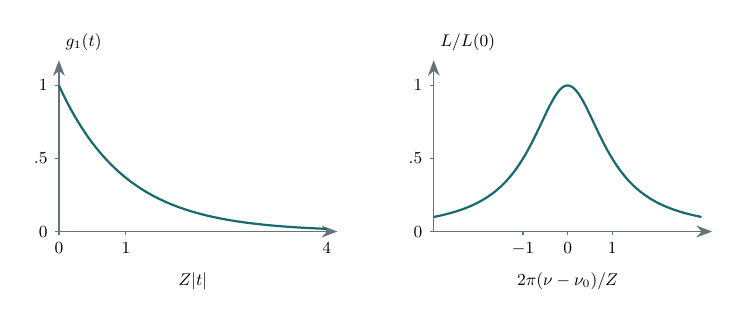
\begin{tikzpicture}[scale=0.68,transform shape]
\draw[axis] (0,0)--(5.2,0);\draw[axis] (0,0)--(0,3.2);
\draw[thin,color=muted] (0.0000000,0)--(0.0000000,-.07);\node[below] at (0.0000000,-.09) {$0$};
\draw[thin,color=muted] (1.2500000,0)--(1.2500000,-.07);\node[below] at (1.2500000,-.09) {$1$};
\draw[thin,color=muted] (5.0000000,0)--(5.0000000,-.07);\node[below] at (5.0000000,-.09) {$4$};
\draw[thin,color=muted] (0,0.0000000)--(-.07,0.0000000);\node[left] at (-.09,0.0000000) {$0$};
\draw[thin,color=muted] (0,1.3636364)--(-.07,1.3636364);\node[left] at (-.09,1.3636364) {$.5$};
\draw[thin,color=muted] (0,2.7272727)--(-.07,2.7272727);\node[left] at (-.09,2.7272727) {$1$};
\node[below] at (2.5,-.64) {$Z|t|$};\node[above right] at (0,3.25) {$g_1(t)$};
\draw[traj] plot coordinates {(0.0000000,2.7272727) (0.0250000,2.6732691) (0.0500000,2.6203348) (0.0750000,2.5684487) (0.1000000,2.5175900) (0.1250000,2.4677384) (0.1500000,2.4188739) (0.1750000,2.3709770) (0.2000000,2.3240285) (0.2250000,2.2780097) (0.2500000,2.2329021) (0.2750000,2.1886876) (0.3000000,2.1453487) (0.3250000,2.1028680) (0.3500000,2.0612284) (0.3750000,2.0204133) (0.4000000,1.9804065) (0.4250000,1.9411918) (0.4500000,1.9027536) (0.4750000,1.8650766) (0.5000000,1.8281456) (0.5250000,1.7919459) (0.5500000,1.7564630) (0.5750000,1.7216827) (0.6000000,1.6875911) (0.6250000,1.6541745) (0.6500000,1.6214197) (0.6750000,1.5893134) (0.7000000,1.5578429) (0.7250000,1.5269955) (0.7500000,1.4967590) (0.7750000,1.4671212) (0.8000000,1.4380702) (0.8250000,1.4095945) (0.8500000,1.3816827) (0.8750000,1.3543236) (0.9000000,1.3275062) (0.9250000,1.3012198) (0.9500000,1.2754539) (0.9750000,1.2501982) (1.0000000,1.2254426) (1.0250000,1.2011772) (1.0500000,1.1773923) (1.0750000,1.1540784) (1.1000000,1.1312261) (1.1250000,1.1088263) (1.1500000,1.0868701) (1.1750000,1.0653486) (1.2000000,1.0442533) (1.2250000,1.0235757) (1.2500000,1.0033076) (1.2750000,0.9834407) (1.3000000,0.9639673) (1.3250000,0.9448795) (1.3500000,0.9261696) (1.3750000,0.9078302) (1.4000000,0.8898540) (1.4250000,0.8722337) (1.4500000,0.8549623) (1.4750000,0.8380329) (1.5000000,0.8214388) (1.5250000,0.8051732) (1.5500000,0.7892297) (1.5750000,0.7736019) (1.6000000,0.7582835) (1.6250000,0.7432685) (1.6500000,0.7285508) (1.6750000,0.7141246) (1.7000000,0.6999839) (1.7250000,0.6861233) (1.7500000,0.6725372) (1.7750000,0.6592200) (1.8000000,0.6461666) (1.8250000,0.6333717) (1.8500000,0.6208301) (1.8750000,0.6085368) (1.9000000,0.5964870) (1.9250000,0.5846757) (1.9500000,0.5730984) (1.9750000,0.5617503) (2.0000000,0.5506269) (2.0250000,0.5397237) (2.0500000,0.5290365) (2.0750000,0.5185609) (2.1000000,0.5082927) (2.1250000,0.4982278) (2.1500000,0.4883622) (2.1750000,0.4786920) (2.2000000,0.4692133) (2.2250000,0.4599222) (2.2500000,0.4508151) (2.2750000,0.4418884) (2.3000000,0.4331384) (2.3250000,0.4245617) (2.3500000,0.4161548) (2.3750000,0.4079144) (2.4000000,0.3998372) (2.4250000,0.3919199) (2.4500000,0.3841593) (2.4750000,0.3765525) (2.5000000,0.3690962) (2.5250000,0.3617876) (2.5500000,0.3546238) (2.5750000,0.3476017) (2.6000000,0.3407188) (2.6250000,0.3339721) (2.6500000,0.3273590) (2.6750000,0.3208768) (2.7000000,0.3145231) (2.7250000,0.3082951) (2.7500000,0.3021904) (2.7750000,0.2962067) (2.8000000,0.2903414) (2.8250000,0.2845922) (2.8500000,0.2789569) (2.8750000,0.2734332) (2.9000000,0.2680189) (2.9250000,0.2627117) (2.9500000,0.2575097) (2.9750000,0.2524107) (3.0000000,0.2474126) (3.0250000,0.2425135) (3.0500000,0.2377114) (3.0750000,0.2330044) (3.1000000,0.2283906) (3.1250000,0.2238682) (3.1500000,0.2194353) (3.1750000,0.2150902) (3.2000000,0.2108311) (3.2250000,0.2066564) (3.2500000,0.2025643) (3.2750000,0.1985533) (3.3000000,0.1946216) (3.3250000,0.1907679) (3.3500000,0.1869904) (3.3750000,0.1832878) (3.4000000,0.1796584) (3.4250000,0.1761009) (3.4500000,0.1726139) (3.4750000,0.1691959) (3.5000000,0.1658456) (3.5250000,0.1625617) (3.5500000,0.1593427) (3.5750000,0.1561875) (3.6000000,0.1530948) (3.6250000,0.1500633) (3.6500000,0.1470919) (3.6750000,0.1441793) (3.7000000,0.1413243) (3.7250000,0.1385259) (3.7500000,0.1357829) (3.7750000,0.1330942) (3.8000000,0.1304588) (3.8250000,0.1278755) (3.8500000,0.1253434) (3.8750000,0.1228615) (3.9000000,0.1204286) (3.9250000,0.1180440) (3.9500000,0.1157066) (3.9750000,0.1134154) (4.0000000,0.1111696) (4.0250000,0.1089683) (4.0500000,0.1068106) (4.0750000,0.1046956) (4.1000000,0.1026225) (4.1250000,0.1005905) (4.1500000,0.0985986) (4.1750000,0.0966462) (4.2000000,0.0947325) (4.2250000,0.0928567) (4.2500000,0.0910180) (4.2750000,0.0892157) (4.3000000,0.0874491) (4.3250000,0.0857175) (4.3500000,0.0840202) (4.3750000,0.0823565) (4.4000000,0.0807257) (4.4250000,0.0791273) (4.4500000,0.0775604) (4.4750000,0.0760246) (4.5000000,0.0745192) (4.5250000,0.0730437) (4.5500000,0.0715973) (4.5750000,0.0701796) (4.6000000,0.0687899) (4.6250000,0.0674278) (4.6500000,0.0660926) (4.6750000,0.0647839) (4.7000000,0.0635011) (4.7250000,0.0622437) (4.7500000,0.0610112) (4.7750000,0.0598031) (4.8000000,0.0586189) (4.8250000,0.0574582) (4.8500000,0.0563204) (4.8750000,0.0552052) (4.9000000,0.0541121) (4.9250000,0.0530406) (4.9500000,0.0519903) (4.9750000,0.0509608) (5.0000000,0.0499517)};
\begin{scope}[xshift=7cm]\draw[axis] (0,0)--(5.2,0);\draw[axis] (0,0)--(0,3.2);
\draw[thin,color=muted] (1.6666667,0)--(1.6666667,-.07);\node[below] at (1.6666667,-.09) {$-1$};
\draw[thin,color=muted] (2.5000000,0)--(2.5000000,-.07);\node[below] at (2.5000000,-.09) {$0$};
\draw[thin,color=muted] (3.3333333,0)--(3.3333333,-.07);\node[below] at (3.3333333,-.09) {$1$};
\draw[thin,color=muted] (0,0.0000000)--(-.07,0.0000000);\node[left] at (-.09,0.0000000) {$0$};
\draw[thin,color=muted] (0,1.3636364)--(-.07,1.3636364);\node[left] at (-.09,1.3636364) {$.5$};
\draw[thin,color=muted] (0,2.7272727)--(-.07,2.7272727);\node[left] at (-.09,2.7272727) {$1$};
\node[below] at (2.5,-.64) {$2\pi(\nu-\nu_0)/Z$};\node[above right] at (0,3.25) {$L/L(0)$};
\draw[traj] plot coordinates {(0.0000000,0.2727273) (0.0166667,0.2760286) (0.0333333,0.2793879) (0.0500000,0.2828065) (0.0666667,0.2862858) (0.0833333,0.2898271) (0.1000000,0.2934318) (0.1166667,0.2971015) (0.1333333,0.3008375) (0.1500000,0.3046415) (0.1666667,0.3085150) (0.1833333,0.3124596) (0.2000000,0.3164771) (0.2166667,0.3205690) (0.2333333,0.3247372) (0.2500000,0.3289834) (0.2666667,0.3333096) (0.2833333,0.3377177) (0.3000000,0.3422095) (0.3166667,0.3467871) (0.3333333,0.3514527) (0.3500000,0.3562082) (0.3666667,0.3610560) (0.3833333,0.3659983) (0.4000000,0.3710373) (0.4166667,0.3761755) (0.4333333,0.3814154) (0.4500000,0.3867594) (0.4666667,0.3922102) (0.4833333,0.3977704) (0.5000000,0.4034427) (0.5166667,0.4092300) (0.5333333,0.4151353) (0.5500000,0.4211614) (0.5666667,0.4273115) (0.5833333,0.4335887) (0.6000000,0.4399962) (0.6166667,0.4465375) (0.6333333,0.4532160) (0.6500000,0.4600352) (0.6666667,0.4669988) (0.6833333,0.4741104) (0.7000000,0.4813740) (0.7166667,0.4887936) (0.7333333,0.4963732) (0.7500000,0.5041170) (0.7666667,0.5120293) (0.7833333,0.5201146) (0.8000000,0.5283774) (0.8166667,0.5368224) (0.8333333,0.5454545) (0.8500000,0.5542787) (0.8666667,0.5632999) (0.8833333,0.5725235) (0.9000000,0.5819547) (0.9166667,0.5915993) (0.9333333,0.6014628) (0.9500000,0.6115510) (0.9666667,0.6218699) (0.9833333,0.6324257) (1.0000000,0.6432247) (1.0166667,0.6542733) (1.0333333,0.6655781) (1.0500000,0.6771459) (1.0666667,0.6889836) (1.0833333,0.7010984) (1.1000000,0.7134975) (1.1166667,0.7261883) (1.1333333,0.7391784) (1.1500000,0.7524756) (1.1666667,0.7660878) (1.1833333,0.7800231) (1.2000000,0.7942896) (1.2166667,0.8088957) (1.2333333,0.8238499) (1.2500000,0.8391608) (1.2666667,0.8548372) (1.2833333,0.8708880) (1.3000000,0.8873219) (1.3166667,0.9041482) (1.3333333,0.9213759) (1.3500000,0.9390142) (1.3666667,0.9570721) (1.3833333,0.9755590) (1.4000000,0.9944839) (1.4166667,1.0138560) (1.4333333,1.0336843) (1.4500000,1.0539777) (1.4666667,1.0747449) (1.4833333,1.0959945) (1.5000000,1.1177347) (1.5166667,1.1399736) (1.5333333,1.1627186) (1.5500000,1.1859770) (1.5666667,1.2097555) (1.5833333,1.2340601) (1.6000000,1.2588962) (1.6166667,1.2842686) (1.6333333,1.3101810) (1.6500000,1.3366363) (1.6666667,1.3636364) (1.6833333,1.3911818) (1.7000000,1.4192718) (1.7166667,1.4479044) (1.7333333,1.4770758) (1.7500000,1.5067805) (1.7666667,1.5370112) (1.7833333,1.5677585) (1.8000000,1.5990107) (1.8166667,1.6307538) (1.8333333,1.6629712) (1.8500000,1.6956433) (1.8666667,1.7287479) (1.8833333,1.7622595) (1.9000000,1.7961491) (1.9166667,1.8303844) (1.9333333,1.8649294) (1.9500000,1.8997442) (1.9666667,1.9347849) (1.9833333,1.9700034) (2.0000000,2.0053476) (2.0166667,2.0407608) (2.0333333,2.0761820) (2.0500000,2.1115459) (2.0666667,2.1467827) (2.0833333,2.1818182) (2.1000000,2.2165741) (2.1166667,2.2509679) (2.1333333,2.2849135) (2.1500000,2.3183209) (2.1666667,2.3510972) (2.1833333,2.3831464) (2.2000000,2.4143703) (2.2166667,2.4446690) (2.2333333,2.4739412) (2.2500000,2.5020851) (2.2666667,2.5289992) (2.2833333,2.5545829) (2.3000000,2.5787375) (2.3166667,2.6013666) (2.3333333,2.6223776) (2.3500000,2.6416822) (2.3666667,2.6591973) (2.3833333,2.6748458) (2.4000000,2.6885575) (2.4166667,2.7002700) (2.4333333,2.7099292) (2.4500000,2.7174898) (2.4666667,2.7229161) (2.4833333,2.7261823) (2.5000000,2.7272727) (2.5166667,2.7261823) (2.5333333,2.7229161) (2.5500000,2.7174898) (2.5666667,2.7099292) (2.5833333,2.7002700) (2.6000000,2.6885575) (2.6166667,2.6748458) (2.6333333,2.6591973) (2.6500000,2.6416822) (2.6666667,2.6223776) (2.6833333,2.6013666) (2.7000000,2.5787375) (2.7166667,2.5545829) (2.7333333,2.5289992) (2.7500000,2.5020851) (2.7666667,2.4739412) (2.7833333,2.4446690) (2.8000000,2.4143703) (2.8166667,2.3831464) (2.8333333,2.3510972) (2.8500000,2.3183209) (2.8666667,2.2849135) (2.8833333,2.2509679) (2.9000000,2.2165741) (2.9166667,2.1818182) (2.9333333,2.1467827) (2.9500000,2.1115459) (2.9666667,2.0761820) (2.9833333,2.0407608) (3.0000000,2.0053476) (3.0166667,1.9700034) (3.0333333,1.9347849) (3.0500000,1.8997442) (3.0666667,1.8649294) (3.0833333,1.8303844) (3.1000000,1.7961491) (3.1166667,1.7622595) (3.1333333,1.7287479) (3.1500000,1.6956433) (3.1666667,1.6629712) (3.1833333,1.6307538) (3.2000000,1.5990107) (3.2166667,1.5677585) (3.2333333,1.5370112) (3.2500000,1.5067805) (3.2666667,1.4770758) (3.2833333,1.4479044) (3.3000000,1.4192718) (3.3166667,1.3911818) (3.3333333,1.3636364) (3.3500000,1.3366363) (3.3666667,1.3101810) (3.3833333,1.2842686) (3.4000000,1.2588962) (3.4166667,1.2340601) (3.4333333,1.2097555) (3.4500000,1.1859770) (3.4666667,1.1627186) (3.4833333,1.1399736) (3.5000000,1.1177347) (3.5166667,1.0959945) (3.5333333,1.0747449) (3.5500000,1.0539777) (3.5666667,1.0336843) (3.5833333,1.0138560) (3.6000000,0.9944839) (3.6166667,0.9755590) (3.6333333,0.9570721) (3.6500000,0.9390142) (3.6666667,0.9213759) (3.6833333,0.9041482) (3.7000000,0.8873219) (3.7166667,0.8708880) (3.7333333,0.8548372) (3.7500000,0.8391608) (3.7666667,0.8238499) (3.7833333,0.8088957) (3.8000000,0.7942896) (3.8166667,0.7800231) (3.8333333,0.7660878) (3.8500000,0.7524756) (3.8666667,0.7391784) (3.8833333,0.7261883) (3.9000000,0.7134975) (3.9166667,0.7010984) (3.9333333,0.6889836) (3.9500000,0.6771459) (3.9666667,0.6655781) (3.9833333,0.6542733) (4.0000000,0.6432247) (4.0166667,0.6324257) (4.0333333,0.6218699) (4.0500000,0.6115510) (4.0666667,0.6014628) (4.0833333,0.5915993) (4.1000000,0.5819547) (4.1166667,0.5725235) (4.1333333,0.5632999) (4.1500000,0.5542787) (4.1666667,0.5454545) (4.1833333,0.5368224) (4.2000000,0.5283774) (4.2166667,0.5201146) (4.2333333,0.5120293) (4.2500000,0.5041170) (4.2666667,0.4963732) (4.2833333,0.4887936) (4.3000000,0.4813740) (4.3166667,0.4741104) (4.3333333,0.4669988) (4.3500000,0.4600352) (4.3666667,0.4532160) (4.3833333,0.4465375) (4.4000000,0.4399962) (4.4166667,0.4335887) (4.4333333,0.4273115) (4.4500000,0.4211614) (4.4666667,0.4151353) (4.4833333,0.4092300) (4.5000000,0.4034427) (4.5166667,0.3977704) (4.5333333,0.3922102) (4.5500000,0.3867594) (4.5666667,0.3814154) (4.5833333,0.3761755) (4.6000000,0.3710373) (4.6166667,0.3659983) (4.6333333,0.3610560) (4.6500000,0.3562082) (4.6666667,0.3514527) (4.6833333,0.3467871) (4.7000000,0.3422095) (4.7166667,0.3377177) (4.7333333,0.3333096) (4.7500000,0.3289834) (4.7666667,0.3247372) (4.7833333,0.3205690) (4.8000000,0.3164771) (4.8166667,0.3124596) (4.8333333,0.3085150) (4.8500000,0.3046415) (4.8666667,0.3008375) (4.8833333,0.2971015) (4.9000000,0.2934318) (4.9166667,0.2898271) (4.9333333,0.2862858) (4.9500000,0.2828065) (4.9666667,0.2793879) (4.9833333,0.2760286) (5.0000000,0.2727273)};
\end{scope}\end{tikzpicture}
\figcaption{解图近试.1C\quad 完全随机化碰撞的指数场相关函数与归一峰高的洛伦兹谱}
\end{minipage}\end{center}


\Needspace{8\baselineskip}

\pdfbookmark[3]{关键洞察}{q1-h5}

\subsection*{关键洞察}

观察方向的正、负速度对称，线性频移后形成单个高斯峰；三维速度密度对横向分量积分后留下一个高斯因子；速率密度中的$v^2$则来自球坐标体积元。热速度控制多普勒方差，碰撞则限制相位保持时间，两种机制分别改变分布和相关函数。比较数值时把峰高定义统一，题设宽度是通常高斯半高全宽的$1/\sqrt2$。

\Needspace{8\baselineskip}

\pdfbookmark[3]{易错点}{q1-h6}

\subsection*{易错点}

速度变量使用一维分量，频率密度含$c/\nu_0$，单位为每赫兹。宽度由两端频率之差给出，单侧偏移为其一半。钠摩尔质量控制多普勒宽度，钠氩约化质量控制平均相对速率；氩数密度由其分压确定。频率增大对应波长减小，波长全宽按两个端点取正差。时间频率的数量级估计与指定洛伦兹线型的$Z/\pi$分别标明。

\Needspace{8\baselineskip}

\pdfbookmark[3]{课堂讲解建议}{q1-h7}

\subsection*{课堂讲解建议}

让学生先画正负速度的高斯分布，逐点对应到红移和蓝移，再用概率小区间解释密度为何乘雅可比。求宽度前在图A上同时画$1/\sqrt2$与$1/2$两条水平线。碰撞部分从图B的扫掠体积推导$Z$，并问氩的质量为什么进入约化质量。最后比较压强加倍与温度加倍分别改变哪些量，再由零碰撞概率导出相关函数，使线型系数有明确的物理过程。

\Needspace{8\baselineskip}

\pdfbookmark[3]{变式训练}{q1-h8}

\subsection*{变式训练}

\begin{enumerate}
\Needspace{37\baselineskip}
\item \textbf{题设与求解。} 将宽度定义改为通常的半高全宽。高斯峰高比$1/2$要求$(\nu-\nu_0)^2/(2\sigma_\nu^2)=\ln2$，故两端相差$W_G=2\sigma_\nu\sqrt{2\ln2}=\sqrt2\Delta\nu_D$。本题相应波长全宽约$1.92\times10^{-3}$纳米。解图近试.1V1在同一高斯曲线上画出两种高度及其横向宽度，系数$\sqrt2$由两个高度的对数比给出。
\begin{center}\begin{minipage}{.98\linewidth}\centering
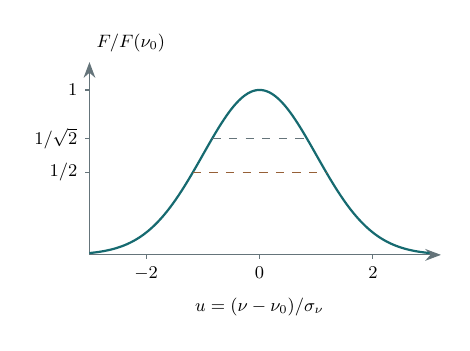
\begin{tikzpicture}[scale=0.72,transform shape]
\draw[axis] (0,0)--(6.2,0);\draw[axis] (0,0)--(0,3.4000000000000004);
\draw[thin,color=muted] (1.0000000,0)--(1.0000000,-.07);\node[below] at (1.0000000,-.09) {$-2$};
\draw[thin,color=muted] (3.0000000,0)--(3.0000000,-.07);\node[below] at (3.0000000,-.09) {$0$};
\draw[thin,color=muted] (5.0000000,0)--(5.0000000,-.07);\node[below] at (5.0000000,-.09) {$2$};
\draw[thin,color=muted] (0,1.4545455)--(-.07,1.4545455);\node[left] at (-.09,1.4545455) {$1/2$};
\draw[thin,color=muted] (0,2.0570379)--(-.07,2.0570379);\node[left] at (-.09,2.0570379) {$1/\sqrt2$};
\draw[thin,color=muted] (0,2.9090909)--(-.07,2.9090909);\node[left] at (-.09,2.9090909) {$1$};
\node[below] at (3.0,-.64) {$u=(\nu-\nu_0)/\sigma_\nu$};\node[above right] at (0,3.45) {$F/F(\nu_0)$};
\draw[traj] plot coordinates {(0.0000000,0.0323171) (0.0150000,0.0338008) (0.0300000,0.0353446) (0.0450000,0.0369507) (0.0600000,0.0386210) (0.0750000,0.0403577) (0.0900000,0.0421631) (0.1050000,0.0440393) (0.1200000,0.0459887) (0.1350000,0.0480136) (0.1500000,0.0501163) (0.1650000,0.0522993) (0.1800000,0.0545652) (0.1950000,0.0569164) (0.2100000,0.0593556) (0.2250000,0.0618853) (0.2400000,0.0645084) (0.2550000,0.0672276) (0.2700000,0.0700456) (0.2850000,0.0729653) (0.3000000,0.0759896) (0.3150000,0.0791214) (0.3300000,0.0823638) (0.3450000,0.0857198) (0.3600000,0.0891924) (0.3750000,0.0927849) (0.3900000,0.0965003) (0.4050000,0.1003419) (0.4200000,0.1043130) (0.4350000,0.1084168) (0.4500000,0.1126568) (0.4650000,0.1170362) (0.4800000,0.1215585) (0.4950000,0.1262272) (0.5100000,0.1310457) (0.5250000,0.1360175) (0.5400000,0.1411462) (0.5550000,0.1464353) (0.5700000,0.1518884) (0.5850000,0.1575091) (0.6000000,0.1633011) (0.6150000,0.1692680) (0.6300000,0.1754135) (0.6450000,0.1817411) (0.6600000,0.1882547) (0.6750000,0.1949579) (0.6900000,0.2018543) (0.7050000,0.2089476) (0.7200000,0.2162415) (0.7350000,0.2237397) (0.7500000,0.2314458) (0.7650000,0.2393635) (0.7800000,0.2474964) (0.7950000,0.2558480) (0.8100000,0.2644219) (0.8250000,0.2732217) (0.8400000,0.2822508) (0.8550000,0.2915127) (0.8700000,0.3010107) (0.8850000,0.3107483) (0.9000000,0.3207288) (0.9150000,0.3309553) (0.9300000,0.3414311) (0.9450000,0.3521592) (0.9600000,0.3631427) (0.9750000,0.3743845) (0.9900000,0.3858875) (1.0050000,0.3976544) (1.0200000,0.4096880) (1.0350000,0.4219908) (1.0500000,0.4345652) (1.0650000,0.4474136) (1.0800000,0.4605382) (1.0950000,0.4739413) (1.1100000,0.4876246) (1.1250000,0.5015902) (1.1400000,0.5158396) (1.1550000,0.5303745) (1.1700000,0.5451963) (1.1850000,0.5603062) (1.2000000,0.5757053) (1.2150000,0.5913946) (1.2300000,0.6073747) (1.2450000,0.6236463) (1.2600000,0.6402098) (1.2750000,0.6570653) (1.2900000,0.6742129) (1.3050000,0.6916523) (1.3200000,0.7093832) (1.3350000,0.7274050) (1.3500000,0.7457168) (1.3650000,0.7643176) (1.3800000,0.7832061) (1.3950000,0.8023809) (1.4100000,0.8218401) (1.4250000,0.8415820) (1.4400000,0.8616041) (1.4550000,0.8819042) (1.4700000,0.9024794) (1.4850000,0.9233270) (1.5000000,0.9444435) (1.5150000,0.9658257) (1.5300000,0.9874698) (1.5450000,1.0093718) (1.5600000,1.0315274) (1.5750000,1.0539322) (1.5900000,1.0765814) (1.6050000,1.0994699) (1.6200000,1.1225924) (1.6350000,1.1459433) (1.6500000,1.1695168) (1.6650000,1.1933066) (1.6800000,1.2173065) (1.6950000,1.2415097) (1.7100000,1.2659092) (1.7250000,1.2904979) (1.7400000,1.3152682) (1.7550000,1.3402124) (1.7700000,1.3653225) (1.7850000,1.3905900) (1.8000000,1.4160066) (1.8150000,1.4415633) (1.8300000,1.4672511) (1.8450000,1.4930606) (1.8600000,1.5189824) (1.8750000,1.5450065) (1.8900000,1.5711230) (1.9050000,1.5973214) (1.9200000,1.6235914) (1.9350000,1.6499222) (1.9500000,1.6763028) (1.9650000,1.7027220) (1.9800000,1.7291685) (1.9950000,1.7556306) (2.0100000,1.7820968) (2.0250000,1.8085549) (2.0400000,1.8349929) (2.0550000,1.8613986) (2.0700000,1.8877594) (2.0850000,1.9140629) (2.1000000,1.9402962) (2.1150000,1.9664465) (2.1300000,1.9925010) (2.1450000,2.0184464) (2.1600000,2.0442697) (2.1750000,2.0699576) (2.1900000,2.0954967) (2.2050000,2.1208737) (2.2200000,2.1460751) (2.2350000,2.1710874) (2.2500000,2.1958970) (2.2650000,2.2204905) (2.2800000,2.2448543) (2.2950000,2.2689749) (2.3100000,2.2928386) (2.3250000,2.3164321) (2.3400000,2.3397419) (2.3550000,2.3627546) (2.3700000,2.3854568) (2.3850000,2.4078353) (2.4000000,2.4298770) (2.4150000,2.4515688) (2.4300000,2.4728977) (2.4450000,2.4938511) (2.4600000,2.5144162) (2.4750000,2.5345805) (2.4900000,2.5543317) (2.5050000,2.5736577) (2.5200000,2.5925466) (2.5350000,2.6109865) (2.5500000,2.6289660) (2.5650000,2.6464738) (2.5800000,2.6634989) (2.5950000,2.6800304) (2.6100000,2.6960578) (2.6250000,2.7115709) (2.6400000,2.7265597) (2.6550000,2.7410146) (2.6700000,2.7549261) (2.6850000,2.7682854) (2.7000000,2.7810836) (2.7150000,2.7933124) (2.7300000,2.8049638) (2.7450000,2.8160301) (2.7600000,2.8265041) (2.7750000,2.8363787) (2.7900000,2.8456475) (2.8050000,2.8543043) (2.8200000,2.8623433) (2.8350000,2.8697592) (2.8500000,2.8765470) (2.8650000,2.8827022) (2.8800000,2.8882207) (2.8950000,2.8930987) (2.9100000,2.8973329) (2.9250000,2.9009206) (2.9400000,2.9038593) (2.9550000,2.9061469) (2.9700000,2.9077821) (2.9850000,2.9087637) (3.0000000,2.9090909) (3.0150000,2.9087637) (3.0300000,2.9077821) (3.0450000,2.9061469) (3.0600000,2.9038593) (3.0750000,2.9009206) (3.0900000,2.8973329) (3.1050000,2.8930987) (3.1200000,2.8882207) (3.1350000,2.8827022) (3.1500000,2.8765470) (3.1650000,2.8697592) (3.1800000,2.8623433) (3.1950000,2.8543043) (3.2100000,2.8456475) (3.2250000,2.8363787) (3.2400000,2.8265041) (3.2550000,2.8160301) (3.2700000,2.8049638) (3.2850000,2.7933124) (3.3000000,2.7810836) (3.3150000,2.7682854) (3.3300000,2.7549261) (3.3450000,2.7410146) (3.3600000,2.7265597) (3.3750000,2.7115709) (3.3900000,2.6960578) (3.4050000,2.6800304) (3.4200000,2.6634989) (3.4350000,2.6464738) (3.4500000,2.6289660) (3.4650000,2.6109865) (3.4800000,2.5925466) (3.4950000,2.5736577) (3.5100000,2.5543317) (3.5250000,2.5345805) (3.5400000,2.5144162) (3.5550000,2.4938511) (3.5700000,2.4728977) (3.5850000,2.4515688) (3.6000000,2.4298770) (3.6150000,2.4078353) (3.6300000,2.3854568) (3.6450000,2.3627546) (3.6600000,2.3397419) (3.6750000,2.3164321) (3.6900000,2.2928386) (3.7050000,2.2689749) (3.7200000,2.2448543) (3.7350000,2.2204905) (3.7500000,2.1958970) (3.7650000,2.1710874) (3.7800000,2.1460751) (3.7950000,2.1208737) (3.8100000,2.0954967) (3.8250000,2.0699576) (3.8400000,2.0442697) (3.8550000,2.0184464) (3.8700000,1.9925010) (3.8850000,1.9664465) (3.9000000,1.9402962) (3.9150000,1.9140629) (3.9300000,1.8877594) (3.9450000,1.8613986) (3.9600000,1.8349929) (3.9750000,1.8085549) (3.9900000,1.7820968) (4.0050000,1.7556306) (4.0200000,1.7291685) (4.0350000,1.7027220) (4.0500000,1.6763028) (4.0650000,1.6499222) (4.0800000,1.6235914) (4.0950000,1.5973214) (4.1100000,1.5711230) (4.1250000,1.5450065) (4.1400000,1.5189824) (4.1550000,1.4930606) (4.1700000,1.4672511) (4.1850000,1.4415633) (4.2000000,1.4160066) (4.2150000,1.3905900) (4.2300000,1.3653225) (4.2450000,1.3402124) (4.2600000,1.3152682) (4.2750000,1.2904979) (4.2900000,1.2659092) (4.3050000,1.2415097) (4.3200000,1.2173065) (4.3350000,1.1933066) (4.3500000,1.1695168) (4.3650000,1.1459433) (4.3800000,1.1225924) (4.3950000,1.0994699) (4.4100000,1.0765814) (4.4250000,1.0539322) (4.4400000,1.0315274) (4.4550000,1.0093718) (4.4700000,0.9874698) (4.4850000,0.9658257) (4.5000000,0.9444435) (4.5150000,0.9233270) (4.5300000,0.9024794) (4.5450000,0.8819042) (4.5600000,0.8616041) (4.5750000,0.8415820) (4.5900000,0.8218401) (4.6050000,0.8023809) (4.6200000,0.7832061) (4.6350000,0.7643176) (4.6500000,0.7457168) (4.6650000,0.7274050) (4.6800000,0.7093832) (4.6950000,0.6916523) (4.7100000,0.6742129) (4.7250000,0.6570653) (4.7400000,0.6402098) (4.7550000,0.6236463) (4.7700000,0.6073747) (4.7850000,0.5913946) (4.8000000,0.5757053) (4.8150000,0.5603062) (4.8300000,0.5451963) (4.8450000,0.5303745) (4.8600000,0.5158396) (4.8750000,0.5015902) (4.8900000,0.4876246) (4.9050000,0.4739413) (4.9200000,0.4605382) (4.9350000,0.4474136) (4.9500000,0.4345652) (4.9650000,0.4219908) (4.9800000,0.4096880) (4.9950000,0.3976544) (5.0100000,0.3858875) (5.0250000,0.3743845) (5.0400000,0.3631427) (5.0550000,0.3521592) (5.0700000,0.3414311) (5.0850000,0.3309553) (5.1000000,0.3207288) (5.1150000,0.3107483) (5.1300000,0.3010107) (5.1450000,0.2915127) (5.1600000,0.2822508) (5.1750000,0.2732217) (5.1900000,0.2644219) (5.2050000,0.2558480) (5.2200000,0.2474964) (5.2350000,0.2393635) (5.2500000,0.2314458) (5.2650000,0.2237397) (5.2800000,0.2162415) (5.2950000,0.2089476) (5.3100000,0.2018543) (5.3250000,0.1949579) (5.3400000,0.1882547) (5.3550000,0.1817411) (5.3700000,0.1754135) (5.3850000,0.1692680) (5.4000000,0.1633011) (5.4150000,0.1575091) (5.4300000,0.1518884) (5.4450000,0.1464353) (5.4600000,0.1411462) (5.4750000,0.1360175) (5.4900000,0.1310457) (5.5050000,0.1262272) (5.5200000,0.1215585) (5.5350000,0.1170362) (5.5500000,0.1126568) (5.5650000,0.1084168) (5.5800000,0.1043130) (5.5950000,0.1003419) (5.6100000,0.0965003) (5.6250000,0.0927849) (5.6400000,0.0891924) (5.6550000,0.0857198) (5.6700000,0.0823638) (5.6850000,0.0791214) (5.7000000,0.0759896) (5.7150000,0.0729653) (5.7300000,0.0700456) (5.7450000,0.0672276) (5.7600000,0.0645084) (5.7750000,0.0618853) (5.7900000,0.0593556) (5.8050000,0.0569164) (5.8200000,0.0545652) (5.8350000,0.0522993) (5.8500000,0.0501163) (5.8650000,0.0480136) (5.8800000,0.0459887) (5.8950000,0.0440393) (5.9100000,0.0421631) (5.9250000,0.0403577) (5.9400000,0.0386210) (5.9550000,0.0369507) (5.9700000,0.0353446) (5.9850000,0.0338008) (6.0000000,0.0323171)};
\draw[dashed,color=warm] (1.82258998,1.45454545)--(4.17741002,1.45454545);\draw[dashed,color=muted] (2.16744539,2.05703791)--(3.83255461,2.05703791);\end{tikzpicture}
\figcaption{解图近试.1V1\quad 两个峰高定义对应不同高斯宽度}
\end{minipage}\end{center}
\Needspace{37\baselineskip}
\item \textbf{题设与求解。} 温度增为四倍，分别讨论压强不变和数密度不变。多普勒宽度总按$\sqrt T$增为两倍。碰撞截面保持时$Z=n\sigma\bar u_{\rm rel}$且$\bar u_{\rm rel}\propto\sqrt T$；定压有$n=p/(k_BT)\propto1/T$，所以$Z\propto p/\sqrt T$，减为一半。定数密度时$Z\propto\sqrt T$，增为两倍。图V2以$T/T_0$作横轴，分别画两种控制条件下的碰撞率比值。
\begin{center}\begin{minipage}{.98\linewidth}\centering
\begin{tikzpicture}[scale=0.72,transform shape]
\draw[axis] (0,0)--(6.2,0);\draw[axis] (0,0)--(0,3.4000000000000004);
\draw[thin,color=muted] (0.0000000,0)--(0.0000000,-.07);\node[below] at (0.0000000,-.09) {$1$};
\draw[thin,color=muted] (2.0000000,0)--(2.0000000,-.07);\node[below] at (2.0000000,-.09) {$2$};
\draw[thin,color=muted] (6.0000000,0)--(6.0000000,-.07);\node[below] at (6.0000000,-.09) {$4$};
\draw[thin,color=muted] (0,0.1882353)--(-.07,0.1882353);\node[left] at (-.09,0.1882353) {$.5$};
\draw[thin,color=muted] (0,1.1294118)--(-.07,1.1294118);\node[left] at (-.09,1.1294118) {$1$};
\draw[thin,color=muted] (0,3.0117647)--(-.07,3.0117647);\node[left] at (-.09,3.0117647) {$2$};
\node[below] at (3.0,-.64) {$T/T_0$};\node[above right] at (0,3.45) {$Z/Z_0$};
\draw[traj] plot coordinates {(0.0000000,1.1294118) (0.0300000,1.1154510) (0.0600000,1.1017963) (0.0900000,1.0884367) (0.1200000,1.0753616) (0.1500000,1.0625612) (0.1800000,1.0500259) (0.2100000,1.0377468) (0.2400000,1.0257152) (0.2700000,1.0139228) (0.3000000,1.0023620) (0.3300000,0.9910251) (0.3600000,0.9799052) (0.3900000,0.9689952) (0.4200000,0.9582888) (0.4500000,0.9477796) (0.4800000,0.9374617) (0.5100000,0.9273293) (0.5400000,0.9173770) (0.5700000,0.9075994) (0.6000000,0.8979916) (0.6300000,0.8885486) (0.6600000,0.8792658) (0.6900000,0.8701388) (0.7200000,0.8611632) (0.7500000,0.8523348) (0.7800000,0.8436497) (0.8100000,0.8351042) (0.8400000,0.8266943) (0.8700000,0.8184167) (0.9000000,0.8102679) (0.9300000,0.8022445) (0.9600000,0.7943434) (0.9900000,0.7865615) (1.0200000,0.7788959) (1.0500000,0.7713437) (1.0800000,0.7639020) (1.1100000,0.7565684) (1.1400000,0.7493400) (1.1700000,0.7422145) (1.2000000,0.7351895) (1.2300000,0.7282625) (1.2600000,0.7214314) (1.2900000,0.7146940) (1.3200000,0.7080480) (1.3500000,0.7014916) (1.3800000,0.6950226) (1.4100000,0.6886392) (1.4400000,0.6823395) (1.4700000,0.6761216) (1.5000000,0.6699839) (1.5300000,0.6639246) (1.5600000,0.6579420) (1.5900000,0.6520346) (1.6200000,0.6462007) (1.6500000,0.6404390) (1.6800000,0.6347478) (1.7100000,0.6291258) (1.7400000,0.6235716) (1.7700000,0.6180838) (1.8000000,0.6126612) (1.8300000,0.6073024) (1.8600000,0.6020061) (1.8900000,0.5967713) (1.9200000,0.5915966) (1.9500000,0.5864811) (1.9800000,0.5814234) (2.0100000,0.5764227) (2.0400000,0.5714777) (2.0700000,0.5665876) (2.1000000,0.5617511) (2.1300000,0.5569675) (2.1600000,0.5522358) (2.1900000,0.5475549) (2.2200000,0.5429240) (2.2500000,0.5383423) (2.2800000,0.5338088) (2.3100000,0.5293227) (2.3400000,0.5248833) (2.3700000,0.5204896) (2.4000000,0.5161409) (2.4300000,0.5118365) (2.4600000,0.5075756) (2.4900000,0.5033574) (2.5200000,0.4991814) (2.5500000,0.4950467) (2.5800000,0.4909527) (2.6100000,0.4868987) (2.6400000,0.4828841) (2.6700000,0.4789082) (2.7000000,0.4749705) (2.7300000,0.4710703) (2.7600000,0.4672070) (2.7900000,0.4633801) (2.8200000,0.4595889) (2.8500000,0.4558330) (2.8800000,0.4521118) (2.9100000,0.4484247) (2.9400000,0.4447713) (2.9700000,0.4411510) (3.0000000,0.4375634) (3.0300000,0.4340078) (3.0600000,0.4304840) (3.0900000,0.4269913) (3.1200000,0.4235294) (3.1500000,0.4200978) (3.1800000,0.4166960) (3.2100000,0.4133237) (3.2400000,0.4099804) (3.2700000,0.4066656) (3.3000000,0.4033790) (3.3300000,0.4001203) (3.3600000,0.3968889) (3.3900000,0.3936845) (3.4200000,0.3905068) (3.4500000,0.3873554) (3.4800000,0.3842298) (3.5100000,0.3811299) (3.5400000,0.3780551) (3.5700000,0.3750052) (3.6000000,0.3719799) (3.6300000,0.3689787) (3.6600000,0.3660015) (3.6900000,0.3630478) (3.7200000,0.3601175) (3.7500000,0.3572100) (3.7800000,0.3543253) (3.8100000,0.3514629) (3.8400000,0.3486226) (3.8700000,0.3458041) (3.9000000,0.3430071) (3.9300000,0.3402313) (3.9600000,0.3374766) (3.9900000,0.3347426) (4.0200000,0.3320290) (4.0500000,0.3293357) (4.0800000,0.3266623) (4.1100000,0.3240086) (4.1400000,0.3213744) (4.1700000,0.3187594) (4.2000000,0.3161635) (4.2300000,0.3135863) (4.2600000,0.3110276) (4.2900000,0.3084873) (4.3200000,0.3059651) (4.3500000,0.3034608) (4.3800000,0.3009741) (4.4100000,0.2985050) (4.4400000,0.2960531) (4.4700000,0.2936183) (4.5000000,0.2912004) (4.5300000,0.2887991) (4.5600000,0.2864144) (4.5900000,0.2840459) (4.6200000,0.2816936) (4.6500000,0.2793572) (4.6800000,0.2770365) (4.7100000,0.2747315) (4.7400000,0.2724418) (4.7700000,0.2701674) (4.8000000,0.2679080) (4.8300000,0.2656636) (4.8600000,0.2634339) (4.8900000,0.2612187) (4.9200000,0.2590180) (4.9500000,0.2568316) (4.9800000,0.2546593) (5.0100000,0.2525009) (5.0400000,0.2503563) (5.0700000,0.2482254) (5.1000000,0.2461080) (5.1300000,0.2440040) (5.1600000,0.2419133) (5.1900000,0.2398356) (5.2200000,0.2377709) (5.2500000,0.2357190) (5.2800000,0.2336798) (5.3100000,0.2316532) (5.3400000,0.2296391) (5.3700000,0.2276372) (5.4000000,0.2256475) (5.4300000,0.2236699) (5.4600000,0.2217042) (5.4900000,0.2197504) (5.5200000,0.2178082) (5.5500000,0.2158777) (5.5800000,0.2139586) (5.6100000,0.2120509) (5.6400000,0.2101544) (5.6700000,0.2082690) (5.7000000,0.2063947) (5.7300000,0.2045313) (5.7600000,0.2026787) (5.7900000,0.2008369) (5.8200000,0.1990056) (5.8500000,0.1971849) (5.8800000,0.1953745) (5.9100000,0.1935745) (5.9400000,0.1917847) (5.9700000,0.1900050) (6.0000000,0.1882353)};
\draw[traj] (.1,-1.05)--(.7,-1.05);\node[right] at (.85,-1.05) {定压碰撞率};\draw[dashed,thick,color=warm] plot coordinates {(0.0000000,1.1294118) (0.0300000,1.1434769) (0.0600000,1.1574384) (0.0900000,1.1712987) (0.1200000,1.1850598) (0.1500000,1.1987239) (0.1800000,1.2122930) (0.2100000,1.2257690) (0.2400000,1.2391539) (0.2700000,1.2524495) (0.3000000,1.2656575) (0.3300000,1.2787796) (0.3600000,1.2918175) (0.3900000,1.3047728) (0.4200000,1.3176471) (0.4500000,1.3304418) (0.4800000,1.3431583) (0.5100000,1.3557983) (0.5400000,1.3683629) (0.5700000,1.3808535) (0.6000000,1.3932714) (0.6300000,1.4056179) (0.6600000,1.4178941) (0.6900000,1.4301014) (0.7200000,1.4422407) (0.7500000,1.4543133) (0.7800000,1.4663202) (0.8100000,1.4782625) (0.8400000,1.4901412) (0.8700000,1.5019574) (0.9000000,1.5137119) (0.9300000,1.5254058) (0.9600000,1.5370400) (0.9900000,1.5486154) (1.0200000,1.5601328) (1.0500000,1.5715932) (1.0800000,1.5829974) (1.1100000,1.5943461) (1.1400000,1.6056403) (1.1700000,1.6168806) (1.2000000,1.6280679) (1.2300000,1.6392028) (1.2600000,1.6502862) (1.2900000,1.6613187) (1.3200000,1.6723009) (1.3500000,1.6832337) (1.3800000,1.6941176) (1.4100000,1.7049534) (1.4400000,1.7157416) (1.4700000,1.7264828) (1.5000000,1.7371777) (1.5300000,1.7478269) (1.5600000,1.7584309) (1.5900000,1.7689903) (1.6200000,1.7795057) (1.6500000,1.7899776) (1.6800000,1.8004066) (1.7100000,1.8107931) (1.7400000,1.8211378) (1.7700000,1.8314410) (1.8000000,1.8417033) (1.8300000,1.8519252) (1.8600000,1.8621071) (1.8900000,1.8722495) (1.9200000,1.8823529) (1.9500000,1.8924178) (1.9800000,1.9024444) (2.0100000,1.9124334) (2.0400000,1.9223850) (2.0700000,1.9322998) (2.1000000,1.9421781) (2.1300000,1.9520203) (2.1600000,1.9618268) (2.1900000,1.9715981) (2.2200000,1.9813344) (2.2500000,1.9910362) (2.2800000,2.0007038) (2.3100000,2.0103376) (2.3400000,2.0199379) (2.3700000,2.0295050) (2.4000000,2.0390394) (2.4300000,2.0485414) (2.4600000,2.0580112) (2.4900000,2.0674492) (2.5200000,2.0768558) (2.5500000,2.0862312) (2.5800000,2.0955757) (2.6100000,2.1048897) (2.6400000,2.1141734) (2.6700000,2.1234272) (2.7000000,2.1326512) (2.7300000,2.1418459) (2.7600000,2.1510115) (2.7900000,2.1601482) (2.8200000,2.1692564) (2.8500000,2.1783363) (2.8800000,2.1873881) (2.9100000,2.1964122) (2.9400000,2.2054087) (2.9700000,2.2143779) (3.0000000,2.2233202) (3.0300000,2.2322356) (3.0600000,2.2411245) (3.0900000,2.2499870) (3.1200000,2.2588235) (3.1500000,2.2676342) (3.1800000,2.2764192) (3.2100000,2.2851788) (3.2400000,2.2939132) (3.2700000,2.3026227) (3.3000000,2.3113074) (3.3300000,2.3199676) (3.3600000,2.3286034) (3.3900000,2.3372151) (3.4200000,2.3458028) (3.4500000,2.3543669) (3.4800000,2.3629074) (3.5100000,2.3714245) (3.5400000,2.3799185) (3.5700000,2.3883895) (3.6000000,2.3968377) (3.6300000,2.4052634) (3.6600000,2.4136666) (3.6900000,2.4220476) (3.7200000,2.4304065) (3.7500000,2.4387435) (3.7800000,2.4470588) (3.8100000,2.4553526) (3.8400000,2.4636249) (3.8700000,2.4718761) (3.9000000,2.4801062) (3.9300000,2.4883154) (3.9600000,2.4965038) (3.9900000,2.5046717) (4.0200000,2.5128191) (4.0500000,2.5209463) (4.0800000,2.5290533) (4.1100000,2.5371404) (4.1400000,2.5452076) (4.1700000,2.5532552) (4.2000000,2.5612832) (4.2300000,2.5692918) (4.2600000,2.5772811) (4.2900000,2.5852514) (4.3200000,2.5932026) (4.3500000,2.6011350) (4.3800000,2.6090487) (4.4100000,2.6169438) (4.4400000,2.6248204) (4.4700000,2.6326787) (4.5000000,2.6405188) (4.5300000,2.6483409) (4.5600000,2.6561450) (4.5900000,2.6639313) (4.6200000,2.6716998) (4.6500000,2.6794508) (4.6800000,2.6871844) (4.7100000,2.6949005) (4.7400000,2.7025995) (4.7700000,2.7102813) (4.8000000,2.7179461) (4.8300000,2.7255941) (4.8600000,2.7332253) (4.8900000,2.7408398) (4.9200000,2.7484377) (4.9500000,2.7560192) (4.9800000,2.7635843) (5.0100000,2.7711332) (5.0400000,2.7786660) (5.0700000,2.7861827) (5.1000000,2.7936835) (5.1300000,2.8011685) (5.1600000,2.8086377) (5.1900000,2.8160913) (5.2200000,2.8235294) (5.2500000,2.8309520) (5.2800000,2.8383593) (5.3100000,2.8457514) (5.3400000,2.8531283) (5.3700000,2.8604901) (5.4000000,2.8678370) (5.4300000,2.8751690) (5.4600000,2.8824862) (5.4900000,2.8897887) (5.5200000,2.8970766) (5.5500000,2.9043500) (5.5800000,2.9116089) (5.6100000,2.9188535) (5.6400000,2.9260838) (5.6700000,2.9333000) (5.7000000,2.9405020) (5.7300000,2.9476900) (5.7600000,2.9548641) (5.7900000,2.9620243) (5.8200000,2.9691708) (5.8500000,2.9763036) (5.8800000,2.9834227) (5.9100000,2.9905283) (5.9400000,2.9976205) (5.9700000,3.0046993) (6.0000000,3.0117647)};
\draw[dashed,thick,color=warm] (.1,-1.48)--(.7,-1.48);\node[right] at (.85,-1.48) {定数密度碰撞率};\end{tikzpicture}
\figcaption{解图近试.1V2\quad 温度改变时，所控制的压强或数密度决定碰撞率的趋势}
\end{minipage}\end{center}
\Needspace{37\baselineskip}
\item \textbf{题设与求解。} 对完全随机化的泊松碰撞，由相关函数求归一化谱与半高全宽。取$\xi=\nu-\nu_0$，\[
L(\xi)=\int_{-\infty}^\infty e^{-Z|t|}e^{-2\pi\mathrm j\xi t}\,\mathrm dt
=2\operatorname{Re}\frac1{Z+2\pi\mathrm j\xi}
=\frac{2Z}{Z^2+(2\pi\xi)^2}.
\]
分母取为峰值处的两倍，得$|\xi|=Z/(2\pi)$，半高全宽为$Z/\pi$。换元$x=2\pi\xi/Z$后密度积分为$\pi^{-1}\int(1+x^2)^{-1}\mathrm dx=1$。图V3标出$x=\pm1$的半高位置，与相关时间$1/Z$对应。
\begin{center}\begin{minipage}{.98\linewidth}\centering
\begin{tikzpicture}[scale=0.72,transform shape]
\draw[axis] (0,0)--(6.2,0);\draw[axis] (0,0)--(0,3.4000000000000004);
\draw[thin,color=muted] (2.0000000,0)--(2.0000000,-.07);\node[below] at (2.0000000,-.09) {$-1$};
\draw[thin,color=muted] (3.0000000,0)--(3.0000000,-.07);\node[below] at (3.0000000,-.09) {$0$};
\draw[thin,color=muted] (4.0000000,0)--(4.0000000,-.07);\node[below] at (4.0000000,-.09) {$1$};
\draw[thin,color=muted] (0,1.4545455)--(-.07,1.4545455);\node[left] at (-.09,1.4545455) {$1/2$};
\draw[thin,color=muted] (0,2.9090909)--(-.07,2.9090909);\node[left] at (-.09,2.9090909) {$1$};
\node[below] at (3.0,-.64) {$2\pi(\nu-\nu_0)/Z$};\node[above right] at (0,3.45) {归一化峰高};
\draw[traj] plot coordinates {(0.0000000,0.2909091) (0.0200000,0.2944305) (0.0400000,0.2980137) (0.0600000,0.3016603) (0.0800000,0.3053715) (0.1000000,0.3091489) (0.1200000,0.3129939) (0.1400000,0.3169082) (0.1600000,0.3208934) (0.1800000,0.3249510) (0.2000000,0.3290827) (0.2200000,0.3332903) (0.2400000,0.3375755) (0.2600000,0.3419403) (0.2800000,0.3463863) (0.3000000,0.3509157) (0.3200000,0.3555303) (0.3400000,0.3602322) (0.3600000,0.3650235) (0.3800000,0.3699063) (0.4000000,0.3748828) (0.4200000,0.3799555) (0.4400000,0.3851264) (0.4600000,0.3903982) (0.4800000,0.3957731) (0.5000000,0.4012539) (0.5200000,0.4068431) (0.5400000,0.4125434) (0.5600000,0.4183575) (0.5800000,0.4242884) (0.6000000,0.4303389) (0.6200000,0.4365121) (0.6400000,0.4428110) (0.6600000,0.4492388) (0.6800000,0.4557989) (0.7000000,0.4624946) (0.7200000,0.4693293) (0.7400000,0.4763067) (0.7600000,0.4834304) (0.7800000,0.4907042) (0.8000000,0.4981320) (0.8200000,0.5057178) (0.8400000,0.5134656) (0.8600000,0.5213798) (0.8800000,0.5294647) (0.9000000,0.5377248) (0.9200000,0.5461646) (0.9400000,0.5547889) (0.9600000,0.5636025) (0.9800000,0.5726106) (1.0000000,0.5818182) (1.0200000,0.5912306) (1.0400000,0.6008532) (1.0600000,0.6106917) (1.0800000,0.6207517) (1.1000000,0.6310392) (1.1200000,0.6415603) (1.1400000,0.6523210) (1.1600000,0.6633279) (1.1800000,0.6745874) (1.2000000,0.6861063) (1.2200000,0.6978915) (1.2400000,0.7099499) (1.2600000,0.7222889) (1.2800000,0.7349159) (1.3000000,0.7478383) (1.3200000,0.7610640) (1.3400000,0.7746008) (1.3600000,0.7884570) (1.3800000,0.8026407) (1.4000000,0.8171604) (1.4200000,0.8320246) (1.4400000,0.8472422) (1.4600000,0.8628221) (1.4800000,0.8787732) (1.5000000,0.8951049) (1.5200000,0.9118264) (1.5400000,0.9289472) (1.5600000,0.9464767) (1.5800000,0.9644248) (1.6000000,0.9828010) (1.6200000,1.0016151) (1.6400000,1.0208769) (1.6600000,1.0405963) (1.6800000,1.0607829) (1.7000000,1.0814464) (1.7200000,1.1025966) (1.7400000,1.1242429) (1.7600000,1.1463946) (1.7800000,1.1690608) (1.8000000,1.1922504) (1.8200000,1.2159718) (1.8400000,1.2402332) (1.8600000,1.2650421) (1.8800000,1.2904058) (1.9000000,1.3163307) (1.9200000,1.3428226) (1.9400000,1.3698865) (1.9600000,1.3975264) (1.9800000,1.4257454) (2.0000000,1.4545455) (2.0200000,1.4839272) (2.0400000,1.5138899) (2.0600000,1.5444314) (2.0800000,1.5755475) (2.1000000,1.6072325) (2.1200000,1.6394786) (2.1400000,1.6722758) (2.1600000,1.7056115) (2.1800000,1.7394708) (2.2000000,1.7738359) (2.2200000,1.8086862) (2.2400000,1.8439978) (2.2600000,1.8797434) (2.2800000,1.9158923) (2.3000000,1.9524100) (2.3200000,1.9892580) (2.3400000,2.0263938) (2.3600000,2.0637705) (2.3800000,2.1013370) (2.4000000,2.1390374) (2.4200000,2.1768115) (2.4400000,2.2145942) (2.4600000,2.2523157) (2.4800000,2.2899015) (2.5000000,2.3272727) (2.5200000,2.3643457) (2.5400000,2.4010324) (2.5600000,2.4372410) (2.5800000,2.4728756) (2.6000000,2.5078370) (2.6200000,2.5420228) (2.6400000,2.5753284) (2.6600000,2.6076469) (2.6800000,2.6388706) (2.7000000,2.6688907) (2.7200000,2.6975991) (2.7400000,2.7248884) (2.7600000,2.7506533) (2.7800000,2.7747910) (2.8000000,2.7972028) (2.8200000,2.8177944) (2.8400000,2.8364771) (2.8600000,2.8531688) (2.8800000,2.8677947) (2.9000000,2.8802880) (2.9200000,2.8905911) (2.9400000,2.8986557) (2.9600000,2.9044438) (2.9800000,2.9079277) (3.0000000,2.9090909) (3.0200000,2.9079277) (3.0400000,2.9044438) (3.0600000,2.8986557) (3.0800000,2.8905911) (3.1000000,2.8802880) (3.1200000,2.8677947) (3.1400000,2.8531688) (3.1600000,2.8364771) (3.1800000,2.8177944) (3.2000000,2.7972028) (3.2200000,2.7747910) (3.2400000,2.7506533) (3.2600000,2.7248884) (3.2800000,2.6975991) (3.3000000,2.6688907) (3.3200000,2.6388706) (3.3400000,2.6076469) (3.3600000,2.5753284) (3.3800000,2.5420228) (3.4000000,2.5078370) (3.4200000,2.4728756) (3.4400000,2.4372410) (3.4600000,2.4010324) (3.4800000,2.3643457) (3.5000000,2.3272727) (3.5200000,2.2899015) (3.5400000,2.2523157) (3.5600000,2.2145942) (3.5800000,2.1768115) (3.6000000,2.1390374) (3.6200000,2.1013370) (3.6400000,2.0637705) (3.6600000,2.0263938) (3.6800000,1.9892580) (3.7000000,1.9524100) (3.7200000,1.9158923) (3.7400000,1.8797434) (3.7600000,1.8439978) (3.7800000,1.8086862) (3.8000000,1.7738359) (3.8200000,1.7394708) (3.8400000,1.7056115) (3.8600000,1.6722758) (3.8800000,1.6394786) (3.9000000,1.6072325) (3.9200000,1.5755475) (3.9400000,1.5444314) (3.9600000,1.5138899) (3.9800000,1.4839272) (4.0000000,1.4545455) (4.0200000,1.4257454) (4.0400000,1.3975264) (4.0600000,1.3698865) (4.0800000,1.3428226) (4.1000000,1.3163307) (4.1200000,1.2904058) (4.1400000,1.2650421) (4.1600000,1.2402332) (4.1800000,1.2159718) (4.2000000,1.1922504) (4.2200000,1.1690608) (4.2400000,1.1463946) (4.2600000,1.1242429) (4.2800000,1.1025966) (4.3000000,1.0814464) (4.3200000,1.0607829) (4.3400000,1.0405963) (4.3600000,1.0208769) (4.3800000,1.0016151) (4.4000000,0.9828010) (4.4200000,0.9644248) (4.4400000,0.9464767) (4.4600000,0.9289472) (4.4800000,0.9118264) (4.5000000,0.8951049) (4.5200000,0.8787732) (4.5400000,0.8628221) (4.5600000,0.8472422) (4.5800000,0.8320246) (4.6000000,0.8171604) (4.6200000,0.8026407) (4.6400000,0.7884570) (4.6600000,0.7746008) (4.6800000,0.7610640) (4.7000000,0.7478383) (4.7200000,0.7349159) (4.7400000,0.7222889) (4.7600000,0.7099499) (4.7800000,0.6978915) (4.8000000,0.6861063) (4.8200000,0.6745874) (4.8400000,0.6633279) (4.8600000,0.6523210) (4.8800000,0.6415603) (4.9000000,0.6310392) (4.9200000,0.6207517) (4.9400000,0.6106917) (4.9600000,0.6008532) (4.9800000,0.5912306) (5.0000000,0.5818182) (5.0200000,0.5726106) (5.0400000,0.5636025) (5.0600000,0.5547889) (5.0800000,0.5461646) (5.1000000,0.5377248) (5.1200000,0.5294647) (5.1400000,0.5213798) (5.1600000,0.5134656) (5.1800000,0.5057178) (5.2000000,0.4981320) (5.2200000,0.4907042) (5.2400000,0.4834304) (5.2600000,0.4763067) (5.2800000,0.4693293) (5.3000000,0.4624946) (5.3200000,0.4557989) (5.3400000,0.4492388) (5.3600000,0.4428110) (5.3800000,0.4365121) (5.4000000,0.4303389) (5.4200000,0.4242884) (5.4400000,0.4183575) (5.4600000,0.4125434) (5.4800000,0.4068431) (5.5000000,0.4012539) (5.5200000,0.3957731) (5.5400000,0.3903982) (5.5600000,0.3851264) (5.5800000,0.3799555) (5.6000000,0.3748828) (5.6200000,0.3699063) (5.6400000,0.3650235) (5.6600000,0.3602322) (5.6800000,0.3555303) (5.7000000,0.3509157) (5.7200000,0.3463863) (5.7400000,0.3419403) (5.7600000,0.3375755) (5.7800000,0.3332903) (5.8000000,0.3290827) (5.8200000,0.3249510) (5.8400000,0.3208934) (5.8600000,0.3169082) (5.8800000,0.3129939) (5.9000000,0.3091489) (5.9200000,0.3053715) (5.9400000,0.3016603) (5.9600000,0.2980137) (5.9800000,0.2944305) (6.0000000,0.2909091)};
\draw[traj] (.1,-1.05)--(.7,-1.05);\node[right] at (.85,-1.05) {洛伦兹谱峰高比};\end{tikzpicture}
\figcaption{解图近试.1V3\quad 半高位置对应频率偏移$Z/(2\pi)$}
\end{minipage}\end{center}
\Needspace{37\baselineskip}
\item \textbf{题设与求解。} 仅将被观察原子的摩尔质量由$\mu$改为$4\mu$，温度、氩质量和数密度保持不变。多普勒方差含$1/\mu$，故宽度减半。碰撞相对速率比为$\sqrt{\mu_{\rm red}/\mu'_{\rm red}}$；对原有钠23克/摩尔、氩40克/摩尔，原约化质量为$23\times40/63$，新值为$92\times40/132$，故比值$\sqrt{11/21}\simeq0.724$。截面保持时碰撞率按这一比例降低。图V4显示两种质量依赖，分别取决于原子本身质量和两体约化质量。
\begin{center}\begin{minipage}{.98\linewidth}\centering
\begin{tikzpicture}[scale=0.72,transform shape]
\draw[axis] (0,0)--(6.2,0);\draw[axis] (0,0)--(0,3.4000000000000004);
\draw[thin,color=muted] (0.0000000,0)--(0.0000000,-.07);\node[below] at (0.0000000,-.09) {$1$};
\draw[thin,color=muted] (2.0000000,0)--(2.0000000,-.07);\node[below] at (2.0000000,-.09) {$2$};
\draw[thin,color=muted] (6.0000000,0)--(6.0000000,-.07);\node[below] at (6.0000000,-.09) {$4$};
\draw[thin,color=muted] (0,0.2666667)--(-.07,0.2666667);\node[left] at (-.09,0.2666667) {$.5$};
\draw[thin,color=muted] (0,1.4613333)--(-.07,1.4613333);\node[left] at (-.09,1.4613333) {$.724$};
\draw[thin,color=muted] (0,2.9333333)--(-.07,2.9333333);\node[left] at (-.09,2.9333333) {$1$};
\node[below] at (3.0,-.64) {被观察原子质量比$\mu/\mu_0$};\node[above right] at (0,3.45) {相对初值};
\draw[traj] plot coordinates {(0.0000000,2.9333333) (0.0300000,2.8937778) (0.0600000,2.8550895) (0.0900000,2.8172372) (0.1200000,2.7801913) (0.1500000,2.7439234) (0.1800000,2.7084069) (0.2100000,2.6736159) (0.2400000,2.6395263) (0.2700000,2.6061147) (0.3000000,2.5733590) (0.3300000,2.5412379) (0.3600000,2.5097313) (0.3900000,2.4788198) (0.4200000,2.4484848) (0.4500000,2.4187088) (0.4800000,2.3894747) (0.5100000,2.3607663) (0.5400000,2.3325681) (0.5700000,2.3048650) (0.6000000,2.2776428) (0.6300000,2.2508877) (0.6600000,2.2245865) (0.6900000,2.1987265) (0.7200000,2.1732956) (0.7500000,2.1482819) (0.7800000,2.1236743) (0.8100000,2.0994618) (0.8400000,2.0756339) (0.8700000,2.0521806) (0.9000000,2.0290923) (0.9300000,2.0063594) (0.9600000,1.9839730) (0.9900000,1.9619244) (1.0200000,1.9402051) (1.0500000,1.9188071) (1.0800000,1.8977225) (1.1100000,1.8769437) (1.1400000,1.8564634) (1.1700000,1.8362745) (1.2000000,1.8163702) (1.2300000,1.7967439) (1.2600000,1.7773891) (1.2900000,1.7582996) (1.3200000,1.7394695) (1.3500000,1.7208928) (1.3800000,1.7025641) (1.4100000,1.6844778) (1.4400000,1.6666285) (1.4700000,1.6490113) (1.5000000,1.6316210) (1.5300000,1.6144530) (1.5600000,1.5975023) (1.5900000,1.5807646) (1.6200000,1.5642354) (1.6500000,1.5479105) (1.6800000,1.5317855) (1.7100000,1.5158565) (1.7400000,1.5001196) (1.7700000,1.4845709) (1.8000000,1.4692067) (1.8300000,1.4540233) (1.8600000,1.4390173) (1.8900000,1.4241853) (1.9200000,1.4095238) (1.9500000,1.3950297) (1.9800000,1.3806998) (2.0100000,1.3665309) (2.0400000,1.3525202) (2.0700000,1.3386647) (2.1000000,1.3249616) (2.1300000,1.3114080) (2.1600000,1.2980013) (2.1900000,1.2847389) (2.2200000,1.2716181) (2.2500000,1.2586365) (2.2800000,1.2457916) (2.3100000,1.2330811) (2.3400000,1.2205026) (2.3700000,1.2080538) (2.4000000,1.1957326) (2.4300000,1.1835368) (2.4600000,1.1714642) (2.4900000,1.1595128) (2.5200000,1.1476806) (2.5500000,1.1359656) (2.5800000,1.1243659) (2.6100000,1.1128796) (2.6400000,1.1015049) (2.6700000,1.0902400) (2.7000000,1.0790831) (2.7300000,1.0680325) (2.7600000,1.0570865) (2.7900000,1.0462436) (2.8200000,1.0355020) (2.8500000,1.0248603) (2.8800000,1.0143168) (2.9100000,1.0038701) (2.9400000,0.9935187) (2.9700000,0.9832612) (3.0000000,0.9730962) (3.0300000,0.9630222) (3.0600000,0.9530379) (3.0900000,0.9431421) (3.1200000,0.9333333) (3.1500000,0.9236104) (3.1800000,0.9139721) (3.2100000,0.9044171) (3.2400000,0.8949443) (3.2700000,0.8855526) (3.3000000,0.8762406) (3.3300000,0.8670074) (3.3600000,0.8578518) (3.3900000,0.8487728) (3.4200000,0.8397693) (3.4500000,0.8308402) (3.4800000,0.8219845) (3.5100000,0.8132012) (3.5400000,0.8044894) (3.5700000,0.7958481) (3.6000000,0.7872763) (3.6300000,0.7787731) (3.6600000,0.7703376) (3.6900000,0.7619689) (3.7200000,0.7536661) (3.7500000,0.7454284) (3.7800000,0.7372549) (3.8100000,0.7291448) (3.8400000,0.7210973) (3.8700000,0.7131115) (3.9000000,0.7051867) (3.9300000,0.6973222) (3.9600000,0.6895170) (3.9900000,0.6817706) (4.0200000,0.6740822) (4.0500000,0.6664511) (4.0800000,0.6588765) (4.1100000,0.6513577) (4.1400000,0.6438941) (4.1700000,0.6364850) (4.2000000,0.6291298) (4.2300000,0.6218277) (4.2600000,0.6145782) (4.2900000,0.6073807) (4.3200000,0.6002344) (4.3500000,0.5931388) (4.3800000,0.5860934) (4.4100000,0.5790975) (4.4400000,0.5721505) (4.4700000,0.5652518) (4.5000000,0.5584010) (4.5300000,0.5515975) (4.5600000,0.5448407) (4.5900000,0.5381301) (4.6200000,0.5314651) (4.6500000,0.5248453) (4.6800000,0.5182702) (4.7100000,0.5117391) (4.7400000,0.5052518) (4.7700000,0.4988076) (4.8000000,0.4924061) (4.8300000,0.4860468) (4.8600000,0.4797293) (4.8900000,0.4734531) (4.9200000,0.4672178) (4.9500000,0.4610228) (4.9800000,0.4548679) (5.0100000,0.4487525) (5.0400000,0.4426762) (5.0700000,0.4366387) (5.1000000,0.4306394) (5.1300000,0.4246781) (5.1600000,0.4187543) (5.1900000,0.4128675) (5.2200000,0.4070175) (5.2500000,0.4012039) (5.2800000,0.3954262) (5.3100000,0.3896842) (5.3400000,0.3839773) (5.3700000,0.3783054) (5.4000000,0.3726680) (5.4300000,0.3670647) (5.4600000,0.3614953) (5.4900000,0.3559594) (5.5200000,0.3504567) (5.5500000,0.3449867) (5.5800000,0.3395493) (5.6100000,0.3341441) (5.6400000,0.3287707) (5.6700000,0.3234289) (5.7000000,0.3181184) (5.7300000,0.3128387) (5.7600000,0.3075898) (5.7900000,0.3023712) (5.8200000,0.2971826) (5.8500000,0.2920238) (5.8800000,0.2868945) (5.9100000,0.2817944) (5.9400000,0.2767233) (5.9700000,0.2716808) (6.0000000,0.2666667)};
\draw[traj] (.1,-1.05)--(.7,-1.05);\node[right] at (.85,-1.05) {多普勒宽度比};\draw[dashed,thick,color=warm] plot coordinates {(0.0000000,2.9333333) (0.0300000,2.9082529) (0.0600000,2.8837890) (0.0900000,2.8599185) (0.1200000,2.8366194) (0.1500000,2.8138706) (0.1800000,2.7916524) (0.2100000,2.7699458) (0.2400000,2.7487327) (0.2700000,2.7279960) (0.3000000,2.7077193) (0.3300000,2.6878871) (0.3600000,2.6684844) (0.3900000,2.6494971) (0.4200000,2.6309115) (0.4500000,2.6127146) (0.4800000,2.5948941) (0.5100000,2.5774381) (0.5400000,2.5603351) (0.5700000,2.5435743) (0.6000000,2.5271452) (0.6300000,2.5110379) (0.6600000,2.4952426) (0.6900000,2.4797503) (0.7200000,2.4645519) (0.7500000,2.4496391) (0.7800000,2.4350036) (0.8100000,2.4206376) (0.8400000,2.4065335) (0.8700000,2.3926841) (0.9000000,2.3790823) (0.9300000,2.3657214) (0.9600000,2.3525949) (0.9900000,2.3396966) (1.0200000,2.3270203) (1.0500000,2.3145604) (1.0800000,2.3023111) (1.1100000,2.2902670) (1.1400000,2.2784230) (1.1700000,2.2667740) (1.2000000,2.2553150) (1.2300000,2.2440414) (1.2600000,2.2329486) (1.2900000,2.2220322) (1.3200000,2.2112879) (1.3500000,2.2007117) (1.3800000,2.1902995) (1.4100000,2.1800474) (1.4400000,2.1699518) (1.4700000,2.1600089) (1.5000000,2.1502153) (1.5300000,2.1405676) (1.5600000,2.1310625) (1.5900000,2.1216967) (1.6200000,2.1124673) (1.6500000,2.1033710) (1.6800000,2.0944052) (1.7100000,2.0855668) (1.7400000,2.0768532) (1.7700000,2.0682617) (1.8000000,2.0597897) (1.8300000,2.0514347) (1.8600000,2.0431942) (1.8900000,2.0350658) (1.9200000,2.0270473) (1.9500000,2.0191363) (1.9800000,2.0113307) (2.0100000,2.0036284) (2.0400000,1.9960273) (2.0700000,1.9885254) (2.1000000,1.9811207) (2.1300000,1.9738113) (2.1600000,1.9665954) (2.1900000,1.9594711) (2.2200000,1.9524366) (2.2500000,1.9454904) (2.2800000,1.9386306) (2.3100000,1.9318557) (2.3400000,1.9251641) (2.3700000,1.9185541) (2.4000000,1.9120244) (2.4300000,1.9055734) (2.4600000,1.8991998) (2.4900000,1.8929020) (2.5200000,1.8866787) (2.5500000,1.8805287) (2.5800000,1.8744505) (2.6100000,1.8684430) (2.6400000,1.8625048) (2.6700000,1.8566348) (2.7000000,1.8508318) (2.7300000,1.8450946) (2.7600000,1.8394222) (2.7900000,1.8338133) (2.8200000,1.8282669) (2.8500000,1.8227820) (2.8800000,1.8173575) (2.9100000,1.8119925) (2.9400000,1.8066859) (2.9700000,1.8014368) (3.0000000,1.7962442) (3.0300000,1.7911073) (3.0600000,1.7860250) (3.0900000,1.7809967) (3.1200000,1.7760212) (3.1500000,1.7710980) (3.1800000,1.7662260) (3.2100000,1.7614045) (3.2400000,1.7566328) (3.2700000,1.7519100) (3.3000000,1.7472353) (3.3300000,1.7426081) (3.3600000,1.7380276) (3.3900000,1.7334931) (3.4200000,1.7290039) (3.4500000,1.7245593) (3.4800000,1.7201587) (3.5100000,1.7158014) (3.5400000,1.7114867) (3.5700000,1.7072140) (3.6000000,1.7029827) (3.6300000,1.6987922) (3.6600000,1.6946419) (3.6900000,1.6905313) (3.7200000,1.6864597) (3.7500000,1.6824266) (3.7800000,1.6784314) (3.8100000,1.6744736) (3.8400000,1.6705527) (3.8700000,1.6666681) (3.9000000,1.6628194) (3.9300000,1.6590061) (3.9600000,1.6552276) (3.9900000,1.6514834) (4.0200000,1.6477732) (4.0500000,1.6440964) (4.0800000,1.6404526) (4.1100000,1.6368414) (4.1400000,1.6332623) (4.1700000,1.6297148) (4.2000000,1.6261986) (4.2300000,1.6227132) (4.2600000,1.6192582) (4.2900000,1.6158333) (4.3200000,1.6124380) (4.3500000,1.6090719) (4.3800000,1.6057347) (4.4100000,1.6024260) (4.4400000,1.5991455) (4.4700000,1.5958927) (4.5000000,1.5926673) (4.5300000,1.5894689) (4.5600000,1.5862973) (4.5900000,1.5831521) (4.6200000,1.5800330) (4.6500000,1.5769395) (4.6800000,1.5738715) (4.7100000,1.5708286) (4.7400000,1.5678104) (4.7700000,1.5648168) (4.8000000,1.5618473) (4.8300000,1.5589017) (4.8600000,1.5559797) (4.8900000,1.5530810) (4.9200000,1.5502054) (4.9500000,1.5473525) (4.9800000,1.5445221) (5.0100000,1.5417139) (5.0400000,1.5389277) (5.0700000,1.5361632) (5.1000000,1.5334201) (5.1300000,1.5306982) (5.1600000,1.5279973) (5.1900000,1.5253170) (5.2200000,1.5226573) (5.2500000,1.5200177) (5.2800000,1.5173982) (5.3100000,1.5147984) (5.3400000,1.5122182) (5.3700000,1.5096573) (5.4000000,1.5071155) (5.4300000,1.5045926) (5.4600000,1.5020883) (5.4900000,1.4996026) (5.5200000,1.4971351) (5.5500000,1.4946857) (5.5800000,1.4922541) (5.6100000,1.4898402) (5.6400000,1.4874438) (5.6700000,1.4850647) (5.7000000,1.4827026) (5.7300000,1.4803575) (5.7600000,1.4780291) (5.7900000,1.4757173) (5.8200000,1.4734218) (5.8500000,1.4711425) (5.8800000,1.4688793) (5.9100000,1.4666319) (5.9400000,1.4644002) (5.9700000,1.4621841) (6.0000000,1.4599833)};
\draw[dashed,thick,color=warm] (.1,-1.48)--(.7,-1.48);\node[right] at (.85,-1.48) {碰撞率比};\end{tikzpicture}
\figcaption{解图近试.1V4\quad 碰撞平均相对速率由两体约化质量控制}
\end{minipage}\end{center}
\Needspace{37\baselineskip}
\item \textbf{题设与求解。} 热速度与碰撞相位过程相互独立，求两种展宽共同作用的线型。单个热速度产生中心频移$\zeta$，碰撞谱在该中心为$L(\xi-\zeta)$；对高斯频移密度平均得到\[
V(\xi)=\int_{-\infty}^{\infty}\frac{e^{-\zeta^2/(2\sigma_\nu^2)}}{\sqrt{2\pi}\sigma_\nu}\,
\frac{2Z}{Z^2+[2\pi(\xi-\zeta)]^2}\,\mathrm d\zeta .
\]
这是高斯与洛伦兹密度的卷积，二者积分均为1，故总谱也归一。时间相关函数相乘为$e^{-2\pi^2\sigma_\nu^2t^2-Z|t|}$。图V5取频率单位$\sigma_\nu$、洛伦兹半高半宽$\gamma=Z/(2\pi)=\sigma_\nu/2$，画出卷积及两个分量；其线型在中心兼有高斯展宽、远尾保留洛伦兹衰减。
\begin{center}\begin{minipage}{.98\linewidth}\centering
\begin{tikzpicture}[scale=0.72,transform shape]
\draw[axis] (0,0)--(6.2,0);\draw[axis] (0,0)--(0,3.4000000000000004);
\draw[thin,color=muted] (0.6000000,0)--(0.6000000,-.07);\node[below] at (0.6000000,-.09) {$-4$};
\draw[thin,color=muted] (3.0000000,0)--(3.0000000,-.07);\node[below] at (3.0000000,-.09) {$0$};
\draw[thin,color=muted] (5.4000000,0)--(5.4000000,-.07);\node[below] at (5.4000000,-.09) {$4$};
\draw[thin,color=muted] (0,0.0000000)--(-.07,0.0000000);\node[left] at (-.09,0.0000000) {$0$};
\draw[thin,color=muted] (0,1.3714286)--(-.07,1.3714286);\node[left] at (-.09,1.3714286) {$.3$};
\draw[thin,color=muted] (0,2.7428571)--(-.07,2.7428571);\node[left] at (-.09,2.7428571) {$.6$};
\node[below] at (3.0,-.64) {$\xi/\sigma_\nu$};\node[above right] at (0,3.45) {频率密度乘$\sigma_\nu$};
\draw[traj] plot coordinates {(0.0000000,0.0331228) (0.0200000,0.0336403) (0.0400000,0.0341710) (0.0600000,0.0347152) (0.0800000,0.0352736) (0.1000000,0.0358467) (0.1200000,0.0364350) (0.1400000,0.0370391) (0.1600000,0.0376597) (0.1800000,0.0382973) (0.2000000,0.0389528) (0.2200000,0.0396267) (0.2400000,0.0403199) (0.2600000,0.0410332) (0.2800000,0.0417674) (0.3000000,0.0425234) (0.3200000,0.0433021) (0.3400000,0.0441046) (0.3600000,0.0449318) (0.3800000,0.0457848) (0.4000000,0.0466649) (0.4200000,0.0475732) (0.4400000,0.0485110) (0.4600000,0.0494797) (0.4800000,0.0504807) (0.5000000,0.0515155) (0.5200000,0.0525858) (0.5400000,0.0536931) (0.5600000,0.0548393) (0.5800000,0.0560263) (0.6000000,0.0572560) (0.6200000,0.0585305) (0.6400000,0.0598521) (0.6600000,0.0612229) (0.6800000,0.0626455) (0.7000000,0.0641224) (0.7200000,0.0656564) (0.7400000,0.0672502) (0.7600000,0.0689069) (0.7800000,0.0706295) (0.8000000,0.0724215) (0.8200000,0.0742863) (0.8400000,0.0762275) (0.8600000,0.0782489) (0.8800000,0.0803545) (0.9000000,0.0825485) (0.9200000,0.0848353) (0.9400000,0.0872195) (0.9600000,0.0897058) (0.9800000,0.0922993) (1.0000000,0.0950051) (1.0200000,0.0978286) (1.0400000,0.1007754) (1.0600000,0.1038515) (1.0800000,0.1070628) (1.1000000,0.1104156) (1.1200000,0.1139165) (1.1400000,0.1175721) (1.1600000,0.1213894) (1.1800000,0.1253756) (1.2000000,0.1295379) (1.2200000,0.1338839) (1.2400000,0.1384213) (1.2600000,0.1431581) (1.2800000,0.1481023) (1.3000000,0.1532622) (1.3200000,0.1586461) (1.3400000,0.1642625) (1.3600000,0.1701200) (1.3800000,0.1762273) (1.4000000,0.1825932) (1.4200000,0.1892263) (1.4400000,0.1961355) (1.4600000,0.2033296) (1.4800000,0.2108171) (1.5000000,0.2186068) (1.5200000,0.2267071) (1.5400000,0.2351263) (1.5600000,0.2438725) (1.5800000,0.2529536) (1.6000000,0.2623771) (1.6200000,0.2721502) (1.6400000,0.2822797) (1.6600000,0.2927721) (1.6800000,0.3036332) (1.7000000,0.3148683) (1.7200000,0.3264822) (1.7400000,0.3384790) (1.7600000,0.3508619) (1.7800000,0.3636336) (1.8000000,0.3767958) (1.8200000,0.3903494) (1.8400000,0.4042944) (1.8600000,0.4186296) (1.8800000,0.4333530) (1.9000000,0.4484613) (1.9200000,0.4639501) (1.9400000,0.4798140) (1.9600000,0.4960460) (1.9800000,0.5126381) (2.0000000,0.5295808) (2.0200000,0.5468635) (2.0400000,0.5644738) (2.0600000,0.5823983) (2.0800000,0.6006219) (2.1000000,0.6191281) (2.1200000,0.6378991) (2.1400000,0.6569154) (2.1600000,0.6761563) (2.1800000,0.6955994) (2.2000000,0.7152212) (2.2200000,0.7349964) (2.2400000,0.7548987) (2.2600000,0.7749003) (2.2800000,0.7949721) (2.3000000,0.8150839) (2.3200000,0.8352043) (2.3400000,0.8553008) (2.3600000,0.8753398) (2.3800000,0.8952869) (2.4000000,0.9151069) (2.4200000,0.9347638) (2.4400000,0.9542210) (2.4600000,0.9734413) (2.4800000,0.9923873) (2.5000000,1.0110211) (2.5200000,1.0293049) (2.5400000,1.0472007) (2.5600000,1.0646707) (2.5800000,1.0816773) (2.6000000,1.0981833) (2.6200000,1.1141522) (2.6400000,1.1295480) (2.6600000,1.1443355) (2.6800000,1.1584806) (2.7000000,1.1719501) (2.7200000,1.1847124) (2.7400000,1.1967367) (2.7600000,1.2079942) (2.7800000,1.2184575) (2.8000000,1.2281008) (2.8200000,1.2369004) (2.8400000,1.2448344) (2.8600000,1.2518829) (2.8800000,1.2580282) (2.9000000,1.2632548) (2.9200000,1.2675493) (2.9400000,1.2709010) (2.9600000,1.2733012) (2.9800000,1.2747437) (3.0000000,1.2752250) (3.0200000,1.2747437) (3.0400000,1.2733012) (3.0600000,1.2709010) (3.0800000,1.2675493) (3.1000000,1.2632548) (3.1200000,1.2580282) (3.1400000,1.2518829) (3.1600000,1.2448344) (3.1800000,1.2369004) (3.2000000,1.2281008) (3.2200000,1.2184575) (3.2400000,1.2079942) (3.2600000,1.1967367) (3.2800000,1.1847124) (3.3000000,1.1719501) (3.3200000,1.1584806) (3.3400000,1.1443355) (3.3600000,1.1295480) (3.3800000,1.1141522) (3.4000000,1.0981833) (3.4200000,1.0816773) (3.4400000,1.0646707) (3.4600000,1.0472007) (3.4800000,1.0293049) (3.5000000,1.0110211) (3.5200000,0.9923873) (3.5400000,0.9734413) (3.5600000,0.9542210) (3.5800000,0.9347638) (3.6000000,0.9151069) (3.6200000,0.8952869) (3.6400000,0.8753398) (3.6600000,0.8553008) (3.6800000,0.8352043) (3.7000000,0.8150839) (3.7200000,0.7949721) (3.7400000,0.7749003) (3.7600000,0.7548987) (3.7800000,0.7349964) (3.8000000,0.7152212) (3.8200000,0.6955994) (3.8400000,0.6761563) (3.8600000,0.6569154) (3.8800000,0.6378991) (3.9000000,0.6191281) (3.9200000,0.6006219) (3.9400000,0.5823983) (3.9600000,0.5644738) (3.9800000,0.5468635) (4.0000000,0.5295808) (4.0200000,0.5126381) (4.0400000,0.4960460) (4.0600000,0.4798140) (4.0800000,0.4639501) (4.1000000,0.4484613) (4.1200000,0.4333530) (4.1400000,0.4186296) (4.1600000,0.4042944) (4.1800000,0.3903494) (4.2000000,0.3767958) (4.2200000,0.3636336) (4.2400000,0.3508619) (4.2600000,0.3384790) (4.2800000,0.3264822) (4.3000000,0.3148683) (4.3200000,0.3036332) (4.3400000,0.2927721) (4.3600000,0.2822797) (4.3800000,0.2721502) (4.4000000,0.2623771) (4.4200000,0.2529536) (4.4400000,0.2438725) (4.4600000,0.2351263) (4.4800000,0.2267071) (4.5000000,0.2186068) (4.5200000,0.2108171) (4.5400000,0.2033296) (4.5600000,0.1961355) (4.5800000,0.1892263) (4.6000000,0.1825932) (4.6200000,0.1762273) (4.6400000,0.1701200) (4.6600000,0.1642625) (4.6800000,0.1586461) (4.7000000,0.1532622) (4.7200000,0.1481023) (4.7400000,0.1431581) (4.7600000,0.1384213) (4.7800000,0.1338839) (4.8000000,0.1295379) (4.8200000,0.1253756) (4.8400000,0.1213894) (4.8600000,0.1175721) (4.8800000,0.1139165) (4.9000000,0.1104156) (4.9200000,0.1070628) (4.9400000,0.1038515) (4.9600000,0.1007754) (4.9800000,0.0978286) (5.0000000,0.0950051) (5.0200000,0.0922993) (5.0400000,0.0897058) (5.0600000,0.0872195) (5.0800000,0.0848353) (5.1000000,0.0825485) (5.1200000,0.0803545) (5.1400000,0.0782489) (5.1600000,0.0762275) (5.1800000,0.0742863) (5.2000000,0.0724215) (5.2200000,0.0706295) (5.2400000,0.0689069) (5.2600000,0.0672502) (5.2800000,0.0656564) (5.3000000,0.0641224) (5.3200000,0.0626455) (5.3400000,0.0612229) (5.3600000,0.0598521) (5.3800000,0.0585305) (5.4000000,0.0572560) (5.4200000,0.0560263) (5.4400000,0.0548393) (5.4600000,0.0536931) (5.4800000,0.0525858) (5.5000000,0.0515155) (5.5200000,0.0504807) (5.5400000,0.0494797) (5.5600000,0.0485110) (5.5800000,0.0475732) (5.6000000,0.0466649) (5.6200000,0.0457848) (5.6400000,0.0449318) (5.6600000,0.0441046) (5.6800000,0.0433021) (5.7000000,0.0425234) (5.7200000,0.0417674) (5.7400000,0.0410332) (5.7600000,0.0403199) (5.7800000,0.0396267) (5.8000000,0.0389528) (5.8200000,0.0382973) (5.8400000,0.0376597) (5.8600000,0.0370391) (5.8800000,0.0364350) (5.9000000,0.0358467) (5.9200000,0.0352736) (5.9400000,0.0347152) (5.9600000,0.0341710) (5.9800000,0.0336403) (6.0000000,0.0331228)};
\draw[traj] (.1,-1.05)--(.7,-1.05);\node[right] at (.85,-1.05) {高斯与洛伦兹卷积};\draw[dashed,thick,color=warm] plot coordinates {(0.0000000,0.0000068) (0.0200000,0.0000080) (0.0400000,0.0000095) (0.0600000,0.0000111) (0.0800000,0.0000131) (0.1000000,0.0000154) (0.1200000,0.0000181) (0.1400000,0.0000212) (0.1600000,0.0000249) (0.1800000,0.0000291) (0.2000000,0.0000340) (0.2200000,0.0000397) (0.2400000,0.0000464) (0.2600000,0.0000540) (0.2800000,0.0000629) (0.3000000,0.0000731) (0.3200000,0.0000848) (0.3400000,0.0000984) (0.3600000,0.0001140) (0.3800000,0.0001320) (0.4000000,0.0001526) (0.4200000,0.0001762) (0.4400000,0.0002032) (0.4600000,0.0002341) (0.4800000,0.0002695) (0.5000000,0.0003098) (0.5200000,0.0003557) (0.5400000,0.0004081) (0.5600000,0.0004676) (0.5800000,0.0005351) (0.6000000,0.0006118) (0.6200000,0.0006987) (0.6400000,0.0007970) (0.6600000,0.0009081) (0.6800000,0.0010336) (0.7000000,0.0011752) (0.7200000,0.0013346) (0.7400000,0.0015140) (0.7600000,0.0017156) (0.7800000,0.0019419) (0.8000000,0.0021955) (0.8200000,0.0024796) (0.8400000,0.0027973) (0.8600000,0.0031522) (0.8800000,0.0035481) (0.9000000,0.0039894) (0.9200000,0.0044806) (0.9400000,0.0050266) (0.9600000,0.0056330) (0.9800000,0.0063055) (1.0000000,0.0070504) (1.0200000,0.0078746) (1.0400000,0.0087854) (1.0600000,0.0097906) (1.0800000,0.0108987) (1.1000000,0.0121187) (1.1200000,0.0134604) (1.1400000,0.0149340) (1.1600000,0.0165506) (1.1800000,0.0183217) (1.2000000,0.0202599) (1.2200000,0.0223782) (1.2400000,0.0246905) (1.2600000,0.0272116) (1.2800000,0.0299567) (1.3000000,0.0329422) (1.3200000,0.0361849) (1.3400000,0.0397027) (1.3600000,0.0435142) (1.3800000,0.0476386) (1.4000000,0.0520959) (1.4200000,0.0569071) (1.4400000,0.0620936) (1.4600000,0.0676775) (1.4800000,0.0736816) (1.5000000,0.0801294) (1.5200000,0.0870446) (1.5400000,0.0944515) (1.5600000,0.1023750) (1.5800000,0.1108399) (1.6000000,0.1198715) (1.6200000,0.1294950) (1.6400000,0.1397358) (1.6600000,0.1506190) (1.6800000,0.1621696) (1.7000000,0.1744120) (1.7200000,0.1873703) (1.7400000,0.2010679) (1.7600000,0.2155272) (1.7800000,0.2307697) (1.8000000,0.2468158) (1.8200000,0.2636846) (1.8400000,0.2813934) (1.8600000,0.2999580) (1.8800000,0.3193923) (1.9000000,0.3397082) (1.9200000,0.3609150) (1.9400000,0.3830199) (1.9600000,0.4060273) (1.9800000,0.4299386) (2.0000000,0.4547526) (2.0200000,0.4804646) (2.0400000,0.5070667) (2.0600000,0.5345473) (2.0800000,0.5628915) (2.1000000,0.5920804) (2.1200000,0.6220913) (2.1400000,0.6528976) (2.1600000,0.6844684) (2.1800000,0.7167690) (2.2000000,0.7497603) (2.2200000,0.7833993) (2.2400000,0.8176385) (2.2600000,0.8524265) (2.2800000,0.8877077) (2.3000000,0.9234226) (2.3200000,0.9595076) (2.3400000,0.9958957) (2.3600000,1.0325158) (2.3800000,1.0692937) (2.4000000,1.1061519) (2.4200000,1.1430098) (2.4400000,1.1797843) (2.4600000,1.2163897) (2.4800000,1.2527381) (2.5000000,1.2887400) (2.5200000,1.3243042) (2.5400000,1.3593387) (2.5600000,1.3937505) (2.5800000,1.4274466) (2.6000000,1.4603337) (2.6200000,1.4923196) (2.6400000,1.5233125) (2.6600000,1.5532223) (2.6800000,1.5819607) (2.7000000,1.6094415) (2.7200000,1.6355814) (2.7400000,1.6603000) (2.7600000,1.6835206) (2.7800000,1.7051703) (2.8000000,1.7251805) (2.8200000,1.7434872) (2.8400000,1.7600314) (2.8600000,1.7747596) (2.8800000,1.7876237) (2.9000000,1.7985816) (2.9200000,1.8075970) (2.9400000,1.8146402) (2.9600000,1.8196879) (2.9800000,1.8227232) (3.0000000,1.8237361) (3.0200000,1.8227232) (3.0400000,1.8196879) (3.0600000,1.8146402) (3.0800000,1.8075970) (3.1000000,1.7985816) (3.1200000,1.7876237) (3.1400000,1.7747596) (3.1600000,1.7600314) (3.1800000,1.7434872) (3.2000000,1.7251805) (3.2200000,1.7051703) (3.2400000,1.6835206) (3.2600000,1.6603000) (3.2800000,1.6355814) (3.3000000,1.6094415) (3.3200000,1.5819607) (3.3400000,1.5532223) (3.3600000,1.5233125) (3.3800000,1.4923196) (3.4000000,1.4603337) (3.4200000,1.4274466) (3.4400000,1.3937505) (3.4600000,1.3593387) (3.4800000,1.3243042) (3.5000000,1.2887400) (3.5200000,1.2527381) (3.5400000,1.2163897) (3.5600000,1.1797843) (3.5800000,1.1430098) (3.6000000,1.1061519) (3.6200000,1.0692937) (3.6400000,1.0325158) (3.6600000,0.9958957) (3.6800000,0.9595076) (3.7000000,0.9234226) (3.7200000,0.8877077) (3.7400000,0.8524265) (3.7600000,0.8176385) (3.7800000,0.7833993) (3.8000000,0.7497603) (3.8200000,0.7167690) (3.8400000,0.6844684) (3.8600000,0.6528976) (3.8800000,0.6220913) (3.9000000,0.5920804) (3.9200000,0.5628915) (3.9400000,0.5345473) (3.9600000,0.5070667) (3.9800000,0.4804646) (4.0000000,0.4547526) (4.0200000,0.4299386) (4.0400000,0.4060273) (4.0600000,0.3830199) (4.0800000,0.3609150) (4.1000000,0.3397082) (4.1200000,0.3193923) (4.1400000,0.2999580) (4.1600000,0.2813934) (4.1800000,0.2636846) (4.2000000,0.2468158) (4.2200000,0.2307697) (4.2400000,0.2155272) (4.2600000,0.2010679) (4.2800000,0.1873703) (4.3000000,0.1744120) (4.3200000,0.1621696) (4.3400000,0.1506190) (4.3600000,0.1397358) (4.3800000,0.1294950) (4.4000000,0.1198715) (4.4200000,0.1108399) (4.4400000,0.1023750) (4.4600000,0.0944515) (4.4800000,0.0870446) (4.5000000,0.0801294) (4.5200000,0.0736816) (4.5400000,0.0676775) (4.5600000,0.0620936) (4.5800000,0.0569071) (4.6000000,0.0520959) (4.6200000,0.0476386) (4.6400000,0.0435142) (4.6600000,0.0397027) (4.6800000,0.0361849) (4.7000000,0.0329422) (4.7200000,0.0299567) (4.7400000,0.0272116) (4.7600000,0.0246905) (4.7800000,0.0223782) (4.8000000,0.0202599) (4.8200000,0.0183217) (4.8400000,0.0165506) (4.8600000,0.0149340) (4.8800000,0.0134604) (4.9000000,0.0121187) (4.9200000,0.0108987) (4.9400000,0.0097906) (4.9600000,0.0087854) (4.9800000,0.0078746) (5.0000000,0.0070504) (5.0200000,0.0063055) (5.0400000,0.0056330) (5.0600000,0.0050266) (5.0800000,0.0044806) (5.1000000,0.0039894) (5.1200000,0.0035481) (5.1400000,0.0031522) (5.1600000,0.0027973) (5.1800000,0.0024796) (5.2000000,0.0021955) (5.2200000,0.0019419) (5.2400000,0.0017156) (5.2600000,0.0015140) (5.2800000,0.0013346) (5.3000000,0.0011752) (5.3200000,0.0010336) (5.3400000,0.0009081) (5.3600000,0.0007970) (5.3800000,0.0006987) (5.4000000,0.0006118) (5.4200000,0.0005351) (5.4400000,0.0004676) (5.4600000,0.0004081) (5.4800000,0.0003557) (5.5000000,0.0003098) (5.5200000,0.0002695) (5.5400000,0.0002341) (5.5600000,0.0002032) (5.5800000,0.0001762) (5.6000000,0.0001526) (5.6200000,0.0001320) (5.6400000,0.0001140) (5.6600000,0.0000984) (5.6800000,0.0000848) (5.7000000,0.0000731) (5.7200000,0.0000629) (5.7400000,0.0000540) (5.7600000,0.0000464) (5.7800000,0.0000397) (5.8000000,0.0000340) (5.8200000,0.0000291) (5.8400000,0.0000249) (5.8600000,0.0000212) (5.8800000,0.0000181) (5.9000000,0.0000154) (5.9200000,0.0000131) (5.9400000,0.0000111) (5.9600000,0.0000095) (5.9800000,0.0000080) (6.0000000,0.0000068)};
\draw[dashed,thick,color=warm] (.1,-1.48)--(.7,-1.48);\node[right] at (.85,-1.48) {高斯分量};\draw[dotted,thick,color=muted] plot coordinates {(0.0000000,0.0288145) (0.0200000,0.0291986) (0.0400000,0.0295905) (0.0600000,0.0299903) (0.0800000,0.0303983) (0.1000000,0.0308145) (0.1200000,0.0312394) (0.1400000,0.0316731) (0.1600000,0.0321158) (0.1800000,0.0325678) (0.2000000,0.0330295) (0.2200000,0.0335009) (0.2400000,0.0339825) (0.2600000,0.0344745) (0.2800000,0.0349772) (0.3000000,0.0354910) (0.3200000,0.0360161) (0.3400000,0.0365529) (0.3600000,0.0371018) (0.3800000,0.0376630) (0.4000000,0.0382370) (0.4200000,0.0388242) (0.4400000,0.0394249) (0.4600000,0.0400397) (0.4800000,0.0406688) (0.5000000,0.0413129) (0.5200000,0.0419722) (0.5400000,0.0426474) (0.5600000,0.0433390) (0.5800000,0.0440474) (0.6000000,0.0447733) (0.6200000,0.0455171) (0.6400000,0.0462795) (0.6600000,0.0470612) (0.6800000,0.0478626) (0.7000000,0.0486847) (0.7200000,0.0495279) (0.7400000,0.0503932) (0.7600000,0.0512811) (0.7800000,0.0521926) (0.8000000,0.0531285) (0.8200000,0.0540896) (0.8400000,0.0550769) (0.8600000,0.0560912) (0.8800000,0.0571337) (0.9000000,0.0582052) (0.9200000,0.0593070) (0.9400000,0.0604402) (0.9600000,0.0616059) (0.9800000,0.0628054) (1.0000000,0.0640400) (1.0200000,0.0653111) (1.0400000,0.0666201) (1.0600000,0.0679685) (1.0800000,0.0693580) (1.1000000,0.0707902) (1.1200000,0.0722667) (1.1400000,0.0737896) (1.1600000,0.0753607) (1.1800000,0.0769820) (1.2000000,0.0786557) (1.2200000,0.0803841) (1.2400000,0.0821695) (1.2600000,0.0840145) (1.2800000,0.0859217) (1.3000000,0.0878938) (1.3200000,0.0899339) (1.3400000,0.0920451) (1.3600000,0.0942307) (1.3800000,0.0964941) (1.4000000,0.0988391) (1.4200000,0.1012695) (1.4400000,0.1037897) (1.4600000,0.1064038) (1.4800000,0.1091166) (1.5000000,0.1119331) (1.5200000,0.1148586) (1.5400000,0.1178986) (1.5600000,0.1210591) (1.5800000,0.1243465) (1.6000000,0.1277676) (1.6200000,0.1313295) (1.6400000,0.1350400) (1.6600000,0.1389073) (1.6800000,0.1429402) (1.7000000,0.1471481) (1.7200000,0.1515411) (1.7400000,0.1561299) (1.7600000,0.1609262) (1.7800000,0.1659425) (1.8000000,0.1711919) (1.8200000,0.1766889) (1.8400000,0.1824488) (1.8600000,0.1884885) (1.8800000,0.1948256) (1.9000000,0.2014797) (1.9200000,0.2084715) (1.9400000,0.2158236) (1.9600000,0.2235606) (1.9800000,0.2317087) (2.0000000,0.2402968) (2.0200000,0.2493560) (2.0400000,0.2589201) (2.0600000,0.2690258) (2.0800000,0.2797133) (2.1000000,0.2910262) (2.1200000,0.3030120) (2.1400000,0.3157227) (2.1600000,0.3292151) (2.1800000,0.3435514) (2.2000000,0.3587994) (2.2200000,0.3750337) (2.2400000,0.3923361) (2.2600000,0.4107961) (2.2800000,0.4305121) (2.3000000,0.4515924) (2.3200000,0.4741556) (2.3400000,0.4983325) (2.3600000,0.5242665) (2.3800000,0.5521154) (2.4000000,0.5820524) (2.4200000,0.6142673) (2.4400000,0.6489682) (2.4600000,0.6863825) (2.4800000,0.7267579) (2.5000000,0.7703634) (2.5200000,0.8174893) (2.5400000,0.8684468) (2.5600000,0.9235669) (2.5800000,0.9831966) (2.6000000,1.0476943) (2.6200000,1.1174213) (2.6400000,1.1927303) (2.6600000,1.2739473) (2.6800000,1.3613491) (2.7000000,1.4551309) (2.7200000,1.5553656) (2.7400000,1.6619515) (2.7600000,1.7745499) (2.7800000,1.8925113) (2.8000000,2.0147966) (2.8200000,2.1398984) (2.8400000,2.2657748) (2.8600000,2.3898135) (2.8800000,2.5088464) (2.9000000,2.6192356) (2.9200000,2.7170494) (2.9400000,2.7983287) (2.9600000,2.8594275) (2.9800000,2.8973846) (3.0000000,2.9102618) (3.0200000,2.8973846) (3.0400000,2.8594275) (3.0600000,2.7983287) (3.0800000,2.7170494) (3.1000000,2.6192356) (3.1200000,2.5088464) (3.1400000,2.3898135) (3.1600000,2.2657748) (3.1800000,2.1398984) (3.2000000,2.0147966) (3.2200000,1.8925113) (3.2400000,1.7745499) (3.2600000,1.6619515) (3.2800000,1.5553656) (3.3000000,1.4551309) (3.3200000,1.3613491) (3.3400000,1.2739473) (3.3600000,1.1927303) (3.3800000,1.1174213) (3.4000000,1.0476943) (3.4200000,0.9831966) (3.4400000,0.9235669) (3.4600000,0.8684468) (3.4800000,0.8174893) (3.5000000,0.7703634) (3.5200000,0.7267579) (3.5400000,0.6863825) (3.5600000,0.6489682) (3.5800000,0.6142673) (3.6000000,0.5820524) (3.6200000,0.5521154) (3.6400000,0.5242665) (3.6600000,0.4983325) (3.6800000,0.4741556) (3.7000000,0.4515924) (3.7200000,0.4305121) (3.7400000,0.4107961) (3.7600000,0.3923361) (3.7800000,0.3750337) (3.8000000,0.3587994) (3.8200000,0.3435514) (3.8400000,0.3292151) (3.8600000,0.3157227) (3.8800000,0.3030120) (3.9000000,0.2910262) (3.9200000,0.2797133) (3.9400000,0.2690258) (3.9600000,0.2589201) (3.9800000,0.2493560) (4.0000000,0.2402968) (4.0200000,0.2317087) (4.0400000,0.2235606) (4.0600000,0.2158236) (4.0800000,0.2084715) (4.1000000,0.2014797) (4.1200000,0.1948256) (4.1400000,0.1884885) (4.1600000,0.1824488) (4.1800000,0.1766889) (4.2000000,0.1711919) (4.2200000,0.1659425) (4.2400000,0.1609262) (4.2600000,0.1561299) (4.2800000,0.1515411) (4.3000000,0.1471481) (4.3200000,0.1429402) (4.3400000,0.1389073) (4.3600000,0.1350400) (4.3800000,0.1313295) (4.4000000,0.1277676) (4.4200000,0.1243465) (4.4400000,0.1210591) (4.4600000,0.1178986) (4.4800000,0.1148586) (4.5000000,0.1119331) (4.5200000,0.1091166) (4.5400000,0.1064038) (4.5600000,0.1037897) (4.5800000,0.1012695) (4.6000000,0.0988391) (4.6200000,0.0964941) (4.6400000,0.0942307) (4.6600000,0.0920451) (4.6800000,0.0899339) (4.7000000,0.0878938) (4.7200000,0.0859217) (4.7400000,0.0840145) (4.7600000,0.0821695) (4.7800000,0.0803841) (4.8000000,0.0786557) (4.8200000,0.0769820) (4.8400000,0.0753607) (4.8600000,0.0737896) (4.8800000,0.0722667) (4.9000000,0.0707902) (4.9200000,0.0693580) (4.9400000,0.0679685) (4.9600000,0.0666201) (4.9800000,0.0653111) (5.0000000,0.0640400) (5.0200000,0.0628054) (5.0400000,0.0616059) (5.0600000,0.0604402) (5.0800000,0.0593070) (5.1000000,0.0582052) (5.1200000,0.0571337) (5.1400000,0.0560912) (5.1600000,0.0550769) (5.1800000,0.0540896) (5.2000000,0.0531285) (5.2200000,0.0521926) (5.2400000,0.0512811) (5.2600000,0.0503932) (5.2800000,0.0495279) (5.3000000,0.0486847) (5.3200000,0.0478626) (5.3400000,0.0470612) (5.3600000,0.0462795) (5.3800000,0.0455171) (5.4000000,0.0447733) (5.4200000,0.0440474) (5.4400000,0.0433390) (5.4600000,0.0426474) (5.4800000,0.0419722) (5.5000000,0.0413129) (5.5200000,0.0406688) (5.5400000,0.0400397) (5.5600000,0.0394249) (5.5800000,0.0388242) (5.6000000,0.0382370) (5.6200000,0.0376630) (5.6400000,0.0371018) (5.6600000,0.0365529) (5.6800000,0.0360161) (5.7000000,0.0354910) (5.7200000,0.0349772) (5.7400000,0.0344745) (5.7600000,0.0339825) (5.7800000,0.0335009) (5.8000000,0.0330295) (5.8200000,0.0325678) (5.8400000,0.0321158) (5.8600000,0.0316731) (5.8800000,0.0312394) (5.9000000,0.0308145) (5.9200000,0.0303983) (5.9400000,0.0299903) (5.9600000,0.0295905) (5.9800000,0.0291986) (6.0000000,0.0288145)};
\draw[dotted,thick,color=muted] (.1,-1.9100000000000001)--(.7,-1.9100000000000001);\node[right] at (.85,-1.9100000000000001) {洛伦兹分量};\end{tikzpicture}
\figcaption{解图近试.1V5\quad 独立热速度与碰撞过程给出归一化卷积谱}
\end{minipage}\end{center}
\Needspace{37\baselineskip}
\item \textbf{题设与求解。} 将窄频率谱严格变换为波长密度。设物理正频率上的归一化密度为$F_+(\nu)$，由$\nu=c/\lambda$及概率守恒，\[
P_\lambda(\lambda)=\frac c{\lambda^2}F_+(c/\lambda),\qquad \lambda>0.
\]
若$F_+$是将中心$\nu_0$、标准差$\sigma_\nu$的高斯在正频率归一后的密度，令$s=\sigma_\nu/\nu_0$、$x=\lambda/\lambda_0$，有$P_\lambda\lambda_0\propto x^{-2}e^{-(1/x-1)^2/(2s^2)}$。对数求导给出$2s^2x^2+x-1=0$，所以峰位$x_{\rm mode}=2/[1+\sqrt{1+8s^2}]\simeq1-2s^2$。图V6为突出变量变换取$s=0.05$，波长密度出现轻微偏斜；本题$s$约$10^{-6}$，一阶宽度变换已足够。
\begin{center}\begin{minipage}{.98\linewidth}\centering
\begin{tikzpicture}[scale=0.72,transform shape]
\draw[axis] (0,0)--(6.2,0);\draw[axis] (0,0)--(0,3.4000000000000004);
\draw[thin,color=muted] (0.5000000,0)--(0.5000000,-.07);\node[below] at (0.5000000,-.09) {$.85$};
\draw[thin,color=muted] (3.0000000,0)--(3.0000000,-.07);\node[below] at (3.0000000,-.09) {$1$};
\draw[thin,color=muted] (5.5000000,0)--(5.5000000,-.07);\node[below] at (5.5000000,-.09) {$1.15$};
\draw[thin,color=muted] (0,0.0000000)--(-.07,0.0000000);\node[left] at (-.09,0.0000000) {$0$};
\draw[thin,color=muted] (0,1.5058824)--(-.07,1.5058824);\node[left] at (-.09,1.5058824) {$4$};
\draw[thin,color=muted] (0,3.0117647)--(-.07,3.0117647);\node[left] at (-.09,3.0117647) {$8$};
\node[below] at (3.0,-.64) {$x=\lambda/\lambda_0$};\node[above right] at (0,3.45) {$P_\lambda\lambda_0$};
\draw[traj] plot coordinates {(0.0000000,0.0002915) (0.0200000,0.0003397) (0.0400000,0.0003952) (0.0600000,0.0004589) (0.0800000,0.0005320) (0.1000000,0.0006157) (0.1200000,0.0007114) (0.1400000,0.0008206) (0.1600000,0.0009450) (0.1800000,0.0010865) (0.2000000,0.0012472) (0.2200000,0.0014294) (0.2400000,0.0016355) (0.2600000,0.0018685) (0.2800000,0.0021313) (0.3000000,0.0024273) (0.3200000,0.0027602) (0.3400000,0.0031338) (0.3600000,0.0035527) (0.3800000,0.0040215) (0.4000000,0.0045454) (0.4200000,0.0051298) (0.4400000,0.0057809) (0.4600000,0.0065051) (0.4800000,0.0073094) (0.5000000,0.0082013) (0.5200000,0.0091889) (0.5400000,0.0102809) (0.5600000,0.0114863) (0.5800000,0.0128152) (0.6000000,0.0142780) (0.6200000,0.0158859) (0.6400000,0.0176506) (0.6600000,0.0195848) (0.6800000,0.0217017) (0.7000000,0.0240153) (0.7200000,0.0265403) (0.7400000,0.0292921) (0.7600000,0.0322871) (0.7800000,0.0355420) (0.8000000,0.0390748) (0.8200000,0.0429037) (0.8400000,0.0470482) (0.8600000,0.0515280) (0.8800000,0.0563638) (0.9000000,0.0615770) (0.9200000,0.0671895) (0.9400000,0.0732240) (0.9600000,0.0797036) (0.9800000,0.0866521) (1.0000000,0.0940938) (1.0200000,0.1020533) (1.0400000,0.1105558) (1.0600000,0.1196266) (1.0800000,0.1292915) (1.1000000,0.1395762) (1.1200000,0.1505067) (1.1400000,0.1621090) (1.1600000,0.1744089) (1.1800000,0.1874322) (1.2000000,0.2012044) (1.2200000,0.2157504) (1.2400000,0.2310949) (1.2600000,0.2472619) (1.2800000,0.2642748) (1.3000000,0.2821559) (1.3200000,0.3009269) (1.3400000,0.3206081) (1.3600000,0.3412190) (1.3800000,0.3627776) (1.4000000,0.3853003) (1.4200000,0.4088023) (1.4400000,0.4332969) (1.4600000,0.4587958) (1.4800000,0.4853085) (1.5000000,0.5128429) (1.5200000,0.5414045) (1.5400000,0.5709966) (1.5600000,0.6016203) (1.5800000,0.6332742) (1.6000000,0.6659545) (1.6200000,0.6996548) (1.6400000,0.7343660) (1.6600000,0.7700763) (1.6800000,0.8067712) (1.7000000,0.8444334) (1.7200000,0.8830427) (1.7400000,0.9225761) (1.7600000,0.9630078) (1.7800000,1.0043090) (1.8000000,1.0464480) (1.8200000,1.0893904) (1.8400000,1.1330988) (1.8600000,1.1775333) (1.8800000,1.2226509) (1.9000000,1.2684063) (1.9200000,1.3147513) (1.9400000,1.3616355) (1.9600000,1.4090058) (1.9800000,1.4568071) (2.0000000,1.5049819) (2.0200000,1.5534706) (2.0400000,1.6022120) (2.0600000,1.6511427) (2.0800000,1.7001982) (2.1000000,1.7493119) (2.1200000,1.7984165) (2.1400000,1.8474433) (2.1600000,1.8963227) (2.1800000,1.9449842) (2.2000000,1.9933571) (2.2200000,2.0413700) (2.2400000,2.0889514) (2.2600000,2.1360298) (2.2800000,2.1825341) (2.3000000,2.2283933) (2.3200000,2.2735373) (2.3400000,2.3178966) (2.3600000,2.3614027) (2.3800000,2.4039885) (2.4000000,2.4455879) (2.4200000,2.4861366) (2.4400000,2.5255720) (2.4600000,2.5638333) (2.4800000,2.6008618) (2.5000000,2.6366010) (2.5200000,2.6709968) (2.5400000,2.7039974) (2.5600000,2.7355538) (2.5800000,2.7656197) (2.6000000,2.7941517) (2.6200000,2.8211091) (2.6400000,2.8464546) (2.6600000,2.8701538) (2.6800000,2.8921755) (2.7000000,2.9124918) (2.7200000,2.9310780) (2.7400000,2.9479130) (2.7600000,2.9629786) (2.7800000,2.9762605) (2.8000000,2.9877473) (2.8200000,2.9974314) (2.8400000,3.0053081) (2.8600000,3.0113764) (2.8800000,3.0156384) (2.9000000,3.0180996) (2.9200000,3.0187684) (2.9400000,3.0176567) (2.9600000,3.0147792) (2.9800000,3.0101537) (3.0000000,3.0038007) (3.0200000,2.9957437) (3.0400000,2.9860088) (3.0600000,2.9746247) (3.0800000,2.9616225) (3.1000000,2.9470359) (3.1200000,2.9309004) (3.1400000,2.9132540) (3.1600000,2.8941366) (3.1800000,2.8735897) (3.2000000,2.8516569) (3.2200000,2.8283831) (3.2400000,2.8038146) (3.2600000,2.7779993) (3.2800000,2.7509860) (3.3000000,2.7228247) (3.3200000,2.6935662) (3.3400000,2.6632620) (3.3600000,2.6319644) (3.3800000,2.5997260) (3.4000000,2.5666000) (3.4200000,2.5326396) (3.4400000,2.4978983) (3.4600000,2.4624295) (3.4800000,2.4262865) (3.5000000,2.3895224) (3.5200000,2.3521899) (3.5400000,2.3143414) (3.5600000,2.2760285) (3.5800000,2.2373024) (3.6000000,2.1982136) (3.6200000,2.1588115) (3.6400000,2.1191448) (3.6600000,2.0792614) (3.6800000,2.0392079) (3.7000000,1.9990299) (3.7200000,1.9587718) (3.7400000,1.9184770) (3.7600000,1.8781873) (3.7800000,1.8379435) (3.8000000,1.7977848) (3.8200000,1.7577493) (3.8400000,1.7178735) (3.8600000,1.6781925) (3.8800000,1.6387401) (3.9000000,1.5995483) (3.9200000,1.5606481) (3.9400000,1.5220686) (3.9600000,1.4838377) (3.9800000,1.4459816) (4.0000000,1.4085251) (4.0200000,1.3714917) (4.0400000,1.3349032) (4.0600000,1.2987800) (4.0800000,1.2631413) (4.1000000,1.2280046) (4.1200000,1.1933862) (4.1400000,1.1593009) (4.1600000,1.1257624) (4.1800000,1.0927828) (4.2000000,1.0603731) (4.2200000,1.0285432) (4.2400000,0.9973015) (4.2600000,0.9666555) (4.2800000,0.9366112) (4.3000000,0.9071741) (4.3200000,0.8783480) (4.3400000,0.8501361) (4.3600000,0.8225406) (4.3800000,0.7955625) (4.4000000,0.7692022) (4.4200000,0.7434590) (4.4400000,0.7183316) (4.4600000,0.6938178) (4.4800000,0.6699147) (4.5000000,0.6466186) (4.5200000,0.6239254) (4.5400000,0.6018301) (4.5600000,0.5803274) (4.5800000,0.5594110) (4.6000000,0.5390747) (4.6200000,0.5193114) (4.6400000,0.5001137) (4.6600000,0.4814737) (4.6800000,0.4633834) (4.7000000,0.4458342) (4.7200000,0.4288173) (4.7400000,0.4123236) (4.7600000,0.3963438) (4.7800000,0.3808684) (4.8000000,0.3658876) (4.8200000,0.3513916) (4.8400000,0.3373704) (4.8600000,0.3238137) (4.8800000,0.3107115) (4.9000000,0.2980534) (4.9200000,0.2858291) (4.9400000,0.2740282) (4.9600000,0.2626405) (4.9800000,0.2516555) (5.0000000,0.2410629) (5.0200000,0.2308525) (5.0400000,0.2210140) (5.0600000,0.2115373) (5.0800000,0.2024123) (5.1000000,0.1936292) (5.1200000,0.1851779) (5.1400000,0.1770487) (5.1600000,0.1692322) (5.1800000,0.1617187) (5.2000000,0.1544989) (5.2200000,0.1475637) (5.2400000,0.1409040) (5.2600000,0.1345110) (5.2800000,0.1283759) (5.3000000,0.1224902) (5.3200000,0.1168455) (5.3400000,0.1114337) (5.3600000,0.1062468) (5.3800000,0.1012769) (5.4000000,0.0965164) (5.4200000,0.0919578) (5.4400000,0.0875940) (5.4600000,0.0834177) (5.4800000,0.0794221) (5.5000000,0.0756005) (5.5200000,0.0719464) (5.5400000,0.0684534) (5.5600000,0.0651153) (5.5800000,0.0619261) (5.6000000,0.0588802) (5.6200000,0.0559717) (5.6400000,0.0531953) (5.6600000,0.0505457) (5.6800000,0.0480178) (5.7000000,0.0456065) (5.7200000,0.0433072) (5.7400000,0.0411152) (5.7600000,0.0390260) (5.7800000,0.0370353) (5.8000000,0.0351390) (5.8200000,0.0333330) (5.8400000,0.0316134) (5.8600000,0.0299765) (5.8800000,0.0284187) (5.9000000,0.0269366) (5.9200000,0.0255268) (5.9400000,0.0241860) (5.9600000,0.0229113) (5.9800000,0.0216996) (6.0000000,0.0205481)};
\draw[traj] (.1,-1.05)--(.7,-1.05);\node[right] at (.85,-1.05) {精确概率变量变换};\draw[dashed,thick,color=warm] plot coordinates {(0.0000000,0.0046073) (0.0200000,0.0050216) (0.0400000,0.0054700) (0.0600000,0.0059551) (0.0800000,0.0064794) (0.1000000,0.0070458) (0.1200000,0.0076573) (0.1400000,0.0083172) (0.1600000,0.0090286) (0.1800000,0.0097953) (0.2000000,0.0106210) (0.2200000,0.0115096) (0.2400000,0.0124655) (0.2600000,0.0134929) (0.2800000,0.0145966) (0.3000000,0.0157814) (0.3200000,0.0170527) (0.3400000,0.0184157) (0.3600000,0.0198762) (0.3800000,0.0214402) (0.4000000,0.0231139) (0.4200000,0.0249039) (0.4400000,0.0268172) (0.4600000,0.0288607) (0.4800000,0.0310421) (0.5000000,0.0333692) (0.5200000,0.0358501) (0.5400000,0.0384932) (0.5600000,0.0413074) (0.5800000,0.0443018) (0.6000000,0.0474859) (0.6200000,0.0508696) (0.6400000,0.0544630) (0.6600000,0.0582767) (0.6800000,0.0623214) (0.7000000,0.0666086) (0.7200000,0.0711497) (0.7400000,0.0759566) (0.7600000,0.0810415) (0.7800000,0.0864171) (0.8000000,0.0920962) (0.8200000,0.0980920) (0.8400000,0.1044180) (0.8600000,0.1110879) (0.8800000,0.1181158) (0.9000000,0.1255161) (0.9200000,0.1333031) (0.9400000,0.1414918) (0.9600000,0.1500970) (0.9800000,0.1591338) (1.0000000,0.1686176) (1.0200000,0.1785637) (1.0400000,0.1889876) (1.0600000,0.1999049) (1.0800000,0.2113310) (1.1000000,0.2232816) (1.1200000,0.2357721) (1.1400000,0.2488180) (1.1600000,0.2624345) (1.1800000,0.2766369) (1.2000000,0.2914399) (1.2200000,0.3068582) (1.2400000,0.3229061) (1.2600000,0.3395977) (1.2800000,0.3569464) (1.3000000,0.3749654) (1.3200000,0.3936671) (1.3400000,0.4130636) (1.3600000,0.4331663) (1.3800000,0.4539857) (1.4000000,0.4755318) (1.4200000,0.4978136) (1.4400000,0.5208394) (1.4600000,0.5446164) (1.4800000,0.5691509) (1.5000000,0.5944483) (1.5200000,0.6205124) (1.5400000,0.6473465) (1.5600000,0.6749521) (1.5800000,0.7033296) (1.6000000,0.7324783) (1.6200000,0.7623957) (1.6400000,0.7930781) (1.6600000,0.8245202) (1.6800000,0.8567153) (1.7000000,0.8896549) (1.7200000,0.9233290) (1.7400000,0.9577259) (1.7600000,0.9928322) (1.7800000,1.0286326) (1.8000000,1.0651103) (1.8200000,1.1022465) (1.8400000,1.1400207) (1.8600000,1.1784104) (1.8800000,1.2173914) (1.9000000,1.2569377) (1.9200000,1.2970214) (1.9400000,1.3376126) (1.9600000,1.3786798) (1.9800000,1.4201896) (2.0000000,1.4621068) (2.0200000,1.5043943) (2.0400000,1.5470136) (2.0600000,1.5899243) (2.0800000,1.6330842) (2.1000000,1.6764499) (2.1200000,1.7199761) (2.1400000,1.7636162) (2.1600000,1.8073224) (2.1800000,1.8510451) (2.2000000,1.8947339) (2.2200000,1.9383370) (2.2400000,1.9818017) (2.2600000,2.0250743) (2.2800000,2.0681002) (2.3000000,2.1108240) (2.3200000,2.1531898) (2.3400000,2.1951412) (2.3600000,2.2366213) (2.3800000,2.2775730) (2.4000000,2.3179389) (2.4200000,2.3576619) (2.4400000,2.3966847) (2.4600000,2.4349504) (2.4800000,2.4724026) (2.5000000,2.5089852) (2.5200000,2.5446431) (2.5400000,2.5793215) (2.5600000,2.6129671) (2.5800000,2.6455273) (2.6000000,2.6769508) (2.6200000,2.7071878) (2.6400000,2.7361898) (2.6600000,2.7639101) (2.6800000,2.7903035) (2.7000000,2.8153269) (2.7200000,2.8389390) (2.7400000,2.8611006) (2.7600000,2.8817749) (2.7800000,2.9009271) (2.8000000,2.9185251) (2.8200000,2.9345390) (2.8400000,2.9489418) (2.8600000,2.9617088) (2.8800000,2.9728182) (2.9000000,2.9822510) (2.9200000,2.9899910) (2.9400000,2.9960249) (2.9600000,3.0003423) (2.9800000,3.0029357) (3.0000000,3.0038007) (3.0200000,3.0029357) (3.0400000,3.0003423) (3.0600000,2.9960249) (3.0800000,2.9899910) (3.1000000,2.9822510) (3.1200000,2.9728182) (3.1400000,2.9617088) (3.1600000,2.9489418) (3.1800000,2.9345390) (3.2000000,2.9185251) (3.2200000,2.9009271) (3.2400000,2.8817749) (3.2600000,2.8611006) (3.2800000,2.8389390) (3.3000000,2.8153269) (3.3200000,2.7903035) (3.3400000,2.7639101) (3.3600000,2.7361898) (3.3800000,2.7071878) (3.4000000,2.6769508) (3.4200000,2.6455273) (3.4400000,2.6129671) (3.4600000,2.5793215) (3.4800000,2.5446431) (3.5000000,2.5089852) (3.5200000,2.4724026) (3.5400000,2.4349504) (3.5600000,2.3966847) (3.5800000,2.3576619) (3.6000000,2.3179389) (3.6200000,2.2775730) (3.6400000,2.2366213) (3.6600000,2.1951412) (3.6800000,2.1531898) (3.7000000,2.1108240) (3.7200000,2.0681002) (3.7400000,2.0250743) (3.7600000,1.9818017) (3.7800000,1.9383370) (3.8000000,1.8947339) (3.8200000,1.8510451) (3.8400000,1.8073224) (3.8600000,1.7636162) (3.8800000,1.7199761) (3.9000000,1.6764499) (3.9200000,1.6330842) (3.9400000,1.5899243) (3.9600000,1.5470136) (3.9800000,1.5043943) (4.0000000,1.4621068) (4.0200000,1.4201896) (4.0400000,1.3786798) (4.0600000,1.3376126) (4.0800000,1.2970214) (4.1000000,1.2569377) (4.1200000,1.2173914) (4.1400000,1.1784104) (4.1600000,1.1400207) (4.1800000,1.1022465) (4.2000000,1.0651103) (4.2200000,1.0286326) (4.2400000,0.9928322) (4.2600000,0.9577259) (4.2800000,0.9233290) (4.3000000,0.8896549) (4.3200000,0.8567153) (4.3400000,0.8245202) (4.3600000,0.7930781) (4.3800000,0.7623957) (4.4000000,0.7324783) (4.4200000,0.7033296) (4.4400000,0.6749521) (4.4600000,0.6473465) (4.4800000,0.6205124) (4.5000000,0.5944483) (4.5200000,0.5691509) (4.5400000,0.5446164) (4.5600000,0.5208394) (4.5800000,0.4978136) (4.6000000,0.4755318) (4.6200000,0.4539857) (4.6400000,0.4331663) (4.6600000,0.4130636) (4.6800000,0.3936671) (4.7000000,0.3749654) (4.7200000,0.3569464) (4.7400000,0.3395977) (4.7600000,0.3229061) (4.7800000,0.3068582) (4.8000000,0.2914399) (4.8200000,0.2766369) (4.8400000,0.2624345) (4.8600000,0.2488180) (4.8800000,0.2357721) (4.9000000,0.2232816) (4.9200000,0.2113310) (4.9400000,0.1999049) (4.9600000,0.1889876) (4.9800000,0.1785637) (5.0000000,0.1686176) (5.0200000,0.1591338) (5.0400000,0.1500970) (5.0600000,0.1414918) (5.0800000,0.1333031) (5.1000000,0.1255161) (5.1200000,0.1181158) (5.1400000,0.1110879) (5.1600000,0.1044180) (5.1800000,0.0980920) (5.2000000,0.0920962) (5.2200000,0.0864171) (5.2400000,0.0810415) (5.2600000,0.0759566) (5.2800000,0.0711497) (5.3000000,0.0666086) (5.3200000,0.0623214) (5.3400000,0.0582767) (5.3600000,0.0544630) (5.3800000,0.0508696) (5.4000000,0.0474859) (5.4200000,0.0443018) (5.4400000,0.0413074) (5.4600000,0.0384932) (5.4800000,0.0358501) (5.5000000,0.0333692) (5.5200000,0.0310421) (5.5400000,0.0288607) (5.5600000,0.0268172) (5.5800000,0.0249039) (5.6000000,0.0231139) (5.6200000,0.0214402) (5.6400000,0.0198762) (5.6600000,0.0184157) (5.6800000,0.0170527) (5.7000000,0.0157814) (5.7200000,0.0145966) (5.7400000,0.0134929) (5.7600000,0.0124655) (5.7800000,0.0115096) (5.8000000,0.0106210) (5.8200000,0.0097953) (5.8400000,0.0090286) (5.8600000,0.0083172) (5.8800000,0.0076573) (5.9000000,0.0070458) (5.9200000,0.0064794) (5.9400000,0.0059551) (5.9600000,0.0054700) (5.9800000,0.0050216) (6.0000000,0.0046073)};
\draw[dashed,thick,color=warm] (.1,-1.48)--(.7,-1.48);\node[right] at (.85,-1.48) {一阶波长高斯近似};\end{tikzpicture}
\figcaption{解图近试.1V6\quad 有限宽度下的波长概率密度含雅可比并出现偏斜}
\end{minipage}\end{center}
\Needspace{37\baselineskip}
\item \textbf{题设与求解。} 同温度、同截面下，提高氩压强到何量级，完全随机化碰撞的半高全宽可与多普勒半高全宽相当？$Z=Z_0p/p_0$，洛伦兹全宽为$Z/\pi$，高斯全宽为$W_G=2\nu_0\sqrt{2RT\ln2/(\mu c^2)}$。令两者相等，得$p_*=\pi W_Gp_0/Z_0$。以$Z_0\simeq5.3\times10^6\,\mathrm{s^{-1}}$和$p_0=10$毫米汞柱估计，$W_G\simeq1.66\times10^9$赫兹，$p_*$约$10^4$毫米汞柱。图V7用$p/p_*$为横轴画两种全宽比；这里沿用定截面的稀气碰撞模型，给出可比较的压强尺度。
\begin{center}\begin{minipage}{.98\linewidth}\centering
\begin{tikzpicture}[scale=0.72,transform shape]
\draw[axis] (0,0)--(6.2,0);\draw[axis] (0,0)--(0,3.4000000000000004);
\draw[thin,color=muted] (0.0000000,0)--(0.0000000,-.07);\node[below] at (0.0000000,-.09) {$0$};
\draw[thin,color=muted] (3.0000000,0)--(3.0000000,-.07);\node[below] at (3.0000000,-.09) {$1$};
\draw[thin,color=muted] (6.0000000,0)--(6.0000000,-.07);\node[below] at (6.0000000,-.09) {$2$};
\draw[thin,color=muted] (0,0.0000000)--(-.07,0.0000000);\node[left] at (-.09,0.0000000) {$0$};
\draw[thin,color=muted] (0,1.5238095)--(-.07,1.5238095);\node[left] at (-.09,1.5238095) {$1$};
\draw[thin,color=muted] (0,3.0476190)--(-.07,3.0476190);\node[left] at (-.09,3.0476190) {$2$};
\node[below] at (3.0,-.64) {$p/p_*$};\node[above right] at (0,3.45) {全宽除以$W_G$};
\draw[traj] plot coordinates {(0.0000000,0.0000000) (0.0300000,0.0152381) (0.0600000,0.0304762) (0.0900000,0.0457143) (0.1200000,0.0609524) (0.1500000,0.0761905) (0.1800000,0.0914286) (0.2100000,0.1066667) (0.2400000,0.1219048) (0.2700000,0.1371429) (0.3000000,0.1523810) (0.3300000,0.1676190) (0.3600000,0.1828571) (0.3900000,0.1980952) (0.4200000,0.2133333) (0.4500000,0.2285714) (0.4800000,0.2438095) (0.5100000,0.2590476) (0.5400000,0.2742857) (0.5700000,0.2895238) (0.6000000,0.3047619) (0.6300000,0.3200000) (0.6600000,0.3352381) (0.6900000,0.3504762) (0.7200000,0.3657143) (0.7500000,0.3809524) (0.7800000,0.3961905) (0.8100000,0.4114286) (0.8400000,0.4266667) (0.8700000,0.4419048) (0.9000000,0.4571429) (0.9300000,0.4723810) (0.9600000,0.4876190) (0.9900000,0.5028571) (1.0200000,0.5180952) (1.0500000,0.5333333) (1.0800000,0.5485714) (1.1100000,0.5638095) (1.1400000,0.5790476) (1.1700000,0.5942857) (1.2000000,0.6095238) (1.2300000,0.6247619) (1.2600000,0.6400000) (1.2900000,0.6552381) (1.3200000,0.6704762) (1.3500000,0.6857143) (1.3800000,0.7009524) (1.4100000,0.7161905) (1.4400000,0.7314286) (1.4700000,0.7466667) (1.5000000,0.7619048) (1.5300000,0.7771429) (1.5600000,0.7923810) (1.5900000,0.8076190) (1.6200000,0.8228571) (1.6500000,0.8380952) (1.6800000,0.8533333) (1.7100000,0.8685714) (1.7400000,0.8838095) (1.7700000,0.8990476) (1.8000000,0.9142857) (1.8300000,0.9295238) (1.8600000,0.9447619) (1.8900000,0.9600000) (1.9200000,0.9752381) (1.9500000,0.9904762) (1.9800000,1.0057143) (2.0100000,1.0209524) (2.0400000,1.0361905) (2.0700000,1.0514286) (2.1000000,1.0666667) (2.1300000,1.0819048) (2.1600000,1.0971429) (2.1900000,1.1123810) (2.2200000,1.1276190) (2.2500000,1.1428571) (2.2800000,1.1580952) (2.3100000,1.1733333) (2.3400000,1.1885714) (2.3700000,1.2038095) (2.4000000,1.2190476) (2.4300000,1.2342857) (2.4600000,1.2495238) (2.4900000,1.2647619) (2.5200000,1.2800000) (2.5500000,1.2952381) (2.5800000,1.3104762) (2.6100000,1.3257143) (2.6400000,1.3409524) (2.6700000,1.3561905) (2.7000000,1.3714286) (2.7300000,1.3866667) (2.7600000,1.4019048) (2.7900000,1.4171429) (2.8200000,1.4323810) (2.8500000,1.4476190) (2.8800000,1.4628571) (2.9100000,1.4780952) (2.9400000,1.4933333) (2.9700000,1.5085714) (3.0000000,1.5238095) (3.0300000,1.5390476) (3.0600000,1.5542857) (3.0900000,1.5695238) (3.1200000,1.5847619) (3.1500000,1.6000000) (3.1800000,1.6152381) (3.2100000,1.6304762) (3.2400000,1.6457143) (3.2700000,1.6609524) (3.3000000,1.6761905) (3.3300000,1.6914286) (3.3600000,1.7066667) (3.3900000,1.7219048) (3.4200000,1.7371429) (3.4500000,1.7523810) (3.4800000,1.7676190) (3.5100000,1.7828571) (3.5400000,1.7980952) (3.5700000,1.8133333) (3.6000000,1.8285714) (3.6300000,1.8438095) (3.6600000,1.8590476) (3.6900000,1.8742857) (3.7200000,1.8895238) (3.7500000,1.9047619) (3.7800000,1.9200000) (3.8100000,1.9352381) (3.8400000,1.9504762) (3.8700000,1.9657143) (3.9000000,1.9809524) (3.9300000,1.9961905) (3.9600000,2.0114286) (3.9900000,2.0266667) (4.0200000,2.0419048) (4.0500000,2.0571429) (4.0800000,2.0723810) (4.1100000,2.0876190) (4.1400000,2.1028571) (4.1700000,2.1180952) (4.2000000,2.1333333) (4.2300000,2.1485714) (4.2600000,2.1638095) (4.2900000,2.1790476) (4.3200000,2.1942857) (4.3500000,2.2095238) (4.3800000,2.2247619) (4.4100000,2.2400000) (4.4400000,2.2552381) (4.4700000,2.2704762) (4.5000000,2.2857143) (4.5300000,2.3009524) (4.5600000,2.3161905) (4.5900000,2.3314286) (4.6200000,2.3466667) (4.6500000,2.3619048) (4.6800000,2.3771429) (4.7100000,2.3923810) (4.7400000,2.4076190) (4.7700000,2.4228571) (4.8000000,2.4380952) (4.8300000,2.4533333) (4.8600000,2.4685714) (4.8900000,2.4838095) (4.9200000,2.4990476) (4.9500000,2.5142857) (4.9800000,2.5295238) (5.0100000,2.5447619) (5.0400000,2.5600000) (5.0700000,2.5752381) (5.1000000,2.5904762) (5.1300000,2.6057143) (5.1600000,2.6209524) (5.1900000,2.6361905) (5.2200000,2.6514286) (5.2500000,2.6666667) (5.2800000,2.6819048) (5.3100000,2.6971429) (5.3400000,2.7123810) (5.3700000,2.7276190) (5.4000000,2.7428571) (5.4300000,2.7580952) (5.4600000,2.7733333) (5.4900000,2.7885714) (5.5200000,2.8038095) (5.5500000,2.8190476) (5.5800000,2.8342857) (5.6100000,2.8495238) (5.6400000,2.8647619) (5.6700000,2.8800000) (5.7000000,2.8952381) (5.7300000,2.9104762) (5.7600000,2.9257143) (5.7900000,2.9409524) (5.8200000,2.9561905) (5.8500000,2.9714286) (5.8800000,2.9866667) (5.9100000,3.0019048) (5.9400000,3.0171429) (5.9700000,3.0323810) (6.0000000,3.0476190)};
\draw[traj] (.1,-1.05)--(.7,-1.05);\node[right] at (.85,-1.05) {碰撞半高全宽};\draw[dashed,thick,color=warm] plot coordinates {(0.0000000,1.5238095) (0.0300000,1.5238095) (0.0600000,1.5238095) (0.0900000,1.5238095) (0.1200000,1.5238095) (0.1500000,1.5238095) (0.1800000,1.5238095) (0.2100000,1.5238095) (0.2400000,1.5238095) (0.2700000,1.5238095) (0.3000000,1.5238095) (0.3300000,1.5238095) (0.3600000,1.5238095) (0.3900000,1.5238095) (0.4200000,1.5238095) (0.4500000,1.5238095) (0.4800000,1.5238095) (0.5100000,1.5238095) (0.5400000,1.5238095) (0.5700000,1.5238095) (0.6000000,1.5238095) (0.6300000,1.5238095) (0.6600000,1.5238095) (0.6900000,1.5238095) (0.7200000,1.5238095) (0.7500000,1.5238095) (0.7800000,1.5238095) (0.8100000,1.5238095) (0.8400000,1.5238095) (0.8700000,1.5238095) (0.9000000,1.5238095) (0.9300000,1.5238095) (0.9600000,1.5238095) (0.9900000,1.5238095) (1.0200000,1.5238095) (1.0500000,1.5238095) (1.0800000,1.5238095) (1.1100000,1.5238095) (1.1400000,1.5238095) (1.1700000,1.5238095) (1.2000000,1.5238095) (1.2300000,1.5238095) (1.2600000,1.5238095) (1.2900000,1.5238095) (1.3200000,1.5238095) (1.3500000,1.5238095) (1.3800000,1.5238095) (1.4100000,1.5238095) (1.4400000,1.5238095) (1.4700000,1.5238095) (1.5000000,1.5238095) (1.5300000,1.5238095) (1.5600000,1.5238095) (1.5900000,1.5238095) (1.6200000,1.5238095) (1.6500000,1.5238095) (1.6800000,1.5238095) (1.7100000,1.5238095) (1.7400000,1.5238095) (1.7700000,1.5238095) (1.8000000,1.5238095) (1.8300000,1.5238095) (1.8600000,1.5238095) (1.8900000,1.5238095) (1.9200000,1.5238095) (1.9500000,1.5238095) (1.9800000,1.5238095) (2.0100000,1.5238095) (2.0400000,1.5238095) (2.0700000,1.5238095) (2.1000000,1.5238095) (2.1300000,1.5238095) (2.1600000,1.5238095) (2.1900000,1.5238095) (2.2200000,1.5238095) (2.2500000,1.5238095) (2.2800000,1.5238095) (2.3100000,1.5238095) (2.3400000,1.5238095) (2.3700000,1.5238095) (2.4000000,1.5238095) (2.4300000,1.5238095) (2.4600000,1.5238095) (2.4900000,1.5238095) (2.5200000,1.5238095) (2.5500000,1.5238095) (2.5800000,1.5238095) (2.6100000,1.5238095) (2.6400000,1.5238095) (2.6700000,1.5238095) (2.7000000,1.5238095) (2.7300000,1.5238095) (2.7600000,1.5238095) (2.7900000,1.5238095) (2.8200000,1.5238095) (2.8500000,1.5238095) (2.8800000,1.5238095) (2.9100000,1.5238095) (2.9400000,1.5238095) (2.9700000,1.5238095) (3.0000000,1.5238095) (3.0300000,1.5238095) (3.0600000,1.5238095) (3.0900000,1.5238095) (3.1200000,1.5238095) (3.1500000,1.5238095) (3.1800000,1.5238095) (3.2100000,1.5238095) (3.2400000,1.5238095) (3.2700000,1.5238095) (3.3000000,1.5238095) (3.3300000,1.5238095) (3.3600000,1.5238095) (3.3900000,1.5238095) (3.4200000,1.5238095) (3.4500000,1.5238095) (3.4800000,1.5238095) (3.5100000,1.5238095) (3.5400000,1.5238095) (3.5700000,1.5238095) (3.6000000,1.5238095) (3.6300000,1.5238095) (3.6600000,1.5238095) (3.6900000,1.5238095) (3.7200000,1.5238095) (3.7500000,1.5238095) (3.7800000,1.5238095) (3.8100000,1.5238095) (3.8400000,1.5238095) (3.8700000,1.5238095) (3.9000000,1.5238095) (3.9300000,1.5238095) (3.9600000,1.5238095) (3.9900000,1.5238095) (4.0200000,1.5238095) (4.0500000,1.5238095) (4.0800000,1.5238095) (4.1100000,1.5238095) (4.1400000,1.5238095) (4.1700000,1.5238095) (4.2000000,1.5238095) (4.2300000,1.5238095) (4.2600000,1.5238095) (4.2900000,1.5238095) (4.3200000,1.5238095) (4.3500000,1.5238095) (4.3800000,1.5238095) (4.4100000,1.5238095) (4.4400000,1.5238095) (4.4700000,1.5238095) (4.5000000,1.5238095) (4.5300000,1.5238095) (4.5600000,1.5238095) (4.5900000,1.5238095) (4.6200000,1.5238095) (4.6500000,1.5238095) (4.6800000,1.5238095) (4.7100000,1.5238095) (4.7400000,1.5238095) (4.7700000,1.5238095) (4.8000000,1.5238095) (4.8300000,1.5238095) (4.8600000,1.5238095) (4.8900000,1.5238095) (4.9200000,1.5238095) (4.9500000,1.5238095) (4.9800000,1.5238095) (5.0100000,1.5238095) (5.0400000,1.5238095) (5.0700000,1.5238095) (5.1000000,1.5238095) (5.1300000,1.5238095) (5.1600000,1.5238095) (5.1900000,1.5238095) (5.2200000,1.5238095) (5.2500000,1.5238095) (5.2800000,1.5238095) (5.3100000,1.5238095) (5.3400000,1.5238095) (5.3700000,1.5238095) (5.4000000,1.5238095) (5.4300000,1.5238095) (5.4600000,1.5238095) (5.4900000,1.5238095) (5.5200000,1.5238095) (5.5500000,1.5238095) (5.5800000,1.5238095) (5.6100000,1.5238095) (5.6400000,1.5238095) (5.6700000,1.5238095) (5.7000000,1.5238095) (5.7300000,1.5238095) (5.7600000,1.5238095) (5.7900000,1.5238095) (5.8200000,1.5238095) (5.8500000,1.5238095) (5.8800000,1.5238095) (5.9100000,1.5238095) (5.9400000,1.5238095) (5.9700000,1.5238095) (6.0000000,1.5238095)};
\draw[dashed,thick,color=warm] (.1,-1.48)--(.7,-1.48);\node[right] at (.85,-1.48) {多普勒半高全宽};\end{tikzpicture}
\figcaption{解图近试.1V7\quad 同一半高定义下，碰撞宽度随定温气体压强增加}
\end{minipage}\end{center}
\Needspace{37\baselineskip}
\item \textbf{题设与求解。} 若每次碰撞后相位因子的平均值为实数$q\in[0,1]$，碰撞仍为率$Z$的泊松过程，求碰撞谱。时间$t$中发生$N$次碰撞的相关因子平均为$q^N$，故\[
g_1(t)=\sum_{N=0}^{\infty}e^{-Z|t|}\frac{(Z|t|)^N}{N!}q^N
=e^{-Z(1-q)|t|}.
\]
傅里叶谱将完全随机化结果中的$Z$替换为$Z(1-q)$，所以半高全宽为$Z(1-q)/\pi$。例如$q=0.8$时线宽为完全随机化的五分之一，而平均碰撞间隔仍为$1/Z$。图V8画线宽与$q$的关系，具体说明碰撞对相位的作用怎样进入系数；$q\to1$时碰撞贡献趋零。
\begin{center}\begin{minipage}{.98\linewidth}\centering
\begin{tikzpicture}[scale=0.72,transform shape]
\draw[axis] (0,0)--(6.2,0);\draw[axis] (0,0)--(0,3.4000000000000004);
\draw[thin,color=muted] (0.0000000,0)--(0.0000000,-.07);\node[below] at (0.0000000,-.09) {$0$};
\draw[thin,color=muted] (4.8000000,0)--(4.8000000,-.07);\node[below] at (4.8000000,-.09) {$.8$};
\draw[thin,color=muted] (6.0000000,0)--(6.0000000,-.07);\node[below] at (6.0000000,-.09) {$1$};
\draw[thin,color=muted] (0,0.0000000)--(-.07,0.0000000);\node[left] at (-.09,0.0000000) {$0$};
\draw[thin,color=muted] (0,0.6095238)--(-.07,0.6095238);\node[left] at (-.09,0.6095238) {$.2$};
\draw[thin,color=muted] (0,3.0476190)--(-.07,3.0476190);\node[left] at (-.09,3.0476190) {$1$};
\node[below] at (3.0,-.64) {平均相位因子$q$};\node[above right] at (0,3.45) {全宽除以$Z/\pi$};
\draw[traj] plot coordinates {(0.0000000,3.0476190) (0.0300000,3.0323810) (0.0600000,3.0171429) (0.0900000,3.0019048) (0.1200000,2.9866667) (0.1500000,2.9714286) (0.1800000,2.9561905) (0.2100000,2.9409524) (0.2400000,2.9257143) (0.2700000,2.9104762) (0.3000000,2.8952381) (0.3300000,2.8800000) (0.3600000,2.8647619) (0.3900000,2.8495238) (0.4200000,2.8342857) (0.4500000,2.8190476) (0.4800000,2.8038095) (0.5100000,2.7885714) (0.5400000,2.7733333) (0.5700000,2.7580952) (0.6000000,2.7428571) (0.6300000,2.7276190) (0.6600000,2.7123810) (0.6900000,2.6971429) (0.7200000,2.6819048) (0.7500000,2.6666667) (0.7800000,2.6514286) (0.8100000,2.6361905) (0.8400000,2.6209524) (0.8700000,2.6057143) (0.9000000,2.5904762) (0.9300000,2.5752381) (0.9600000,2.5600000) (0.9900000,2.5447619) (1.0200000,2.5295238) (1.0500000,2.5142857) (1.0800000,2.4990476) (1.1100000,2.4838095) (1.1400000,2.4685714) (1.1700000,2.4533333) (1.2000000,2.4380952) (1.2300000,2.4228571) (1.2600000,2.4076190) (1.2900000,2.3923810) (1.3200000,2.3771429) (1.3500000,2.3619048) (1.3800000,2.3466667) (1.4100000,2.3314286) (1.4400000,2.3161905) (1.4700000,2.3009524) (1.5000000,2.2857143) (1.5300000,2.2704762) (1.5600000,2.2552381) (1.5900000,2.2400000) (1.6200000,2.2247619) (1.6500000,2.2095238) (1.6800000,2.1942857) (1.7100000,2.1790476) (1.7400000,2.1638095) (1.7700000,2.1485714) (1.8000000,2.1333333) (1.8300000,2.1180952) (1.8600000,2.1028571) (1.8900000,2.0876190) (1.9200000,2.0723810) (1.9500000,2.0571429) (1.9800000,2.0419048) (2.0100000,2.0266667) (2.0400000,2.0114286) (2.0700000,1.9961905) (2.1000000,1.9809524) (2.1300000,1.9657143) (2.1600000,1.9504762) (2.1900000,1.9352381) (2.2200000,1.9200000) (2.2500000,1.9047619) (2.2800000,1.8895238) (2.3100000,1.8742857) (2.3400000,1.8590476) (2.3700000,1.8438095) (2.4000000,1.8285714) (2.4300000,1.8133333) (2.4600000,1.7980952) (2.4900000,1.7828571) (2.5200000,1.7676190) (2.5500000,1.7523810) (2.5800000,1.7371429) (2.6100000,1.7219048) (2.6400000,1.7066667) (2.6700000,1.6914286) (2.7000000,1.6761905) (2.7300000,1.6609524) (2.7600000,1.6457143) (2.7900000,1.6304762) (2.8200000,1.6152381) (2.8500000,1.6000000) (2.8800000,1.5847619) (2.9100000,1.5695238) (2.9400000,1.5542857) (2.9700000,1.5390476) (3.0000000,1.5238095) (3.0300000,1.5085714) (3.0600000,1.4933333) (3.0900000,1.4780952) (3.1200000,1.4628571) (3.1500000,1.4476190) (3.1800000,1.4323810) (3.2100000,1.4171429) (3.2400000,1.4019048) (3.2700000,1.3866667) (3.3000000,1.3714286) (3.3300000,1.3561905) (3.3600000,1.3409524) (3.3900000,1.3257143) (3.4200000,1.3104762) (3.4500000,1.2952381) (3.4800000,1.2800000) (3.5100000,1.2647619) (3.5400000,1.2495238) (3.5700000,1.2342857) (3.6000000,1.2190476) (3.6300000,1.2038095) (3.6600000,1.1885714) (3.6900000,1.1733333) (3.7200000,1.1580952) (3.7500000,1.1428571) (3.7800000,1.1276190) (3.8100000,1.1123810) (3.8400000,1.0971429) (3.8700000,1.0819048) (3.9000000,1.0666667) (3.9300000,1.0514286) (3.9600000,1.0361905) (3.9900000,1.0209524) (4.0200000,1.0057143) (4.0500000,0.9904762) (4.0800000,0.9752381) (4.1100000,0.9600000) (4.1400000,0.9447619) (4.1700000,0.9295238) (4.2000000,0.9142857) (4.2300000,0.8990476) (4.2600000,0.8838095) (4.2900000,0.8685714) (4.3200000,0.8533333) (4.3500000,0.8380952) (4.3800000,0.8228571) (4.4100000,0.8076190) (4.4400000,0.7923810) (4.4700000,0.7771429) (4.5000000,0.7619048) (4.5300000,0.7466667) (4.5600000,0.7314286) (4.5900000,0.7161905) (4.6200000,0.7009524) (4.6500000,0.6857143) (4.6800000,0.6704762) (4.7100000,0.6552381) (4.7400000,0.6400000) (4.7700000,0.6247619) (4.8000000,0.6095238) (4.8300000,0.5942857) (4.8600000,0.5790476) (4.8900000,0.5638095) (4.9200000,0.5485714) (4.9500000,0.5333333) (4.9800000,0.5180952) (5.0100000,0.5028571) (5.0400000,0.4876190) (5.0700000,0.4723810) (5.1000000,0.4571429) (5.1300000,0.4419048) (5.1600000,0.4266667) (5.1900000,0.4114286) (5.2200000,0.3961905) (5.2500000,0.3809524) (5.2800000,0.3657143) (5.3100000,0.3504762) (5.3400000,0.3352381) (5.3700000,0.3200000) (5.4000000,0.3047619) (5.4300000,0.2895238) (5.4600000,0.2742857) (5.4900000,0.2590476) (5.5200000,0.2438095) (5.5500000,0.2285714) (5.5800000,0.2133333) (5.6100000,0.1980952) (5.6400000,0.1828571) (5.6700000,0.1676190) (5.7000000,0.1523810) (5.7300000,0.1371429) (5.7600000,0.1219048) (5.7900000,0.1066667) (5.8200000,0.0914286) (5.8500000,0.0761905) (5.8800000,0.0609524) (5.9100000,0.0457143) (5.9400000,0.0304762) (5.9700000,0.0152381) (6.0000000,0.0000000)};
\draw[traj] (.1,-1.05)--(.7,-1.05);\node[right] at (.85,-1.05) {相位记忆后的碰撞线宽};\end{tikzpicture}
\figcaption{解图近试.1V8\quad 每次碰撞保留的相位相关越大，碰撞贡献的线宽越小}
\end{minipage}\end{center}
\end{enumerate}

\Needspace{13\baselineskip}

\pdfbookmark[2]{第 2 题 中子干涉中的重力相位差}{q2}

\section*{第 2 题\quad 中子干涉中的重力相位差}\label{q:2}


四个光路结点$B,C,E,D$构成菱形，$BC=CE=ED=DB=l$，对角线$BE$分别与$BC$、$BD$夹角$\theta$。平行单晶片在$B$分束，使两束低能中子分别沿$BCE$与$BDE$传播，在$E$合束后由探测器$F$计数。

装置平面$S$可绕$BD$轴旋转，相对水平面$S_0$的有向夹角为$\phi\in[-90^\circ,90^\circ]$；规定$\phi>0$时$C,E$高于$B,D$。重力势能变化远小于中子初动能，忽略光路的微小重力弯曲。
\begin{enumerate}
\item 证明重力相位差可写成$\delta=q\sin\phi$、$q=k\lambda l^2\sin2\theta$，求常数$k$；相位差定义为下路径减上路径，$\lambda$为入射波长。
\item 初动能为$3.9\times10^{-2}\,\mathrm{eV}$，$l=4.0\,\mathrm{cm}$、$\theta=22.5^\circ$，估计旋转全程相长极大的次数。分别说明固定附加相位未知，以及已校准$\phi=0$为相长极大时的答案。
\end{enumerate}
可用中子静能$mc^2=939\,\mathrm{MeV}$、$\hbar c=1.97\times10^{-11}\,\mathrm{MeV\,cm}$、$g=9.8\,\mathrm{m/s^2}$。


\begin{center}\begin{minipage}{.98\linewidth}\centering
\begin{tikzpicture}[scale=.65,transform shape]

\coordinate (B) at (0,0);\coordinate (D) at (4,0);
\coordinate (C) at (2.828,2.828);\coordinate (E) at (6.828,2.828);
\draw[object] (B)--(C)--(E)--(D)--cycle;
\draw[guide,line width=1.2pt] (B)--(E);
\draw[guide,line width=1.2pt] (2.2,2.568)--(3.456,3.088);
\draw[guide,line width=1.2pt] (3.372,-.26)--(4.628,.26);
\draw[motion] (-1.5,0)--(B) node[midway,above] {$A$};
\draw[motion] (C)--(4.8,2.828);
\draw[motion] (D)--(5.6,1.6);
\draw[motion] (E)--(8,2.828) node[right] {$F$};
\foreach \p/\pos in {B/below left,C/above left,E/above,D/below right}{\fill (\p) circle (1.5pt) node[\pos] {$\p$};}
\node[below] at (2,0) {$l$};\node[above] at (4.8,2.828) {$l$};
\node[left] at (1.4,1.5) {$l$};\node[right] at (5.6,1.5) {$l$};
\draw[object] (1.2,0) arc[start angle=0,end angle=22.5,radius=1.2];
\draw[object] (22.5:1.6) arc[start angle=22.5,end angle=45,radius=1.6];
\node at (1.4,.2) {$\theta$};\node at (1.65,1.05) {$\theta$};
\begin{scope}[xshift=10cm]
\draw[guide] (-1,0)--(3,0) node[right] {$S_0$};
\draw[object] (0,0)--(2.5,1.5) node[right] {$S$};
\fill (0,0) circle (2pt) node[below] {$BD$轴};
\node at (1,.3) {$\phi$};
\end{scope}

\end{tikzpicture}
\figcaption{图近试.2\quad 菱形光路的平面内几何与绕BD旋转的侧视示意。}
\end{minipage}\end{center}

\Needspace{8\baselineskip}

\pdfbookmark[3]{题型定位}{q2-h0}

\subsection*{题型定位}

定能量物质波在重力场中的空间相位与有限转角内的相长计数。先配对高度历程相同的斜边，再由高、低水平段的动量差求相位；最后保留固定晶体相位，按可达相位区间中的整数点计数。

\Needspace{8\baselineskip}

\pdfbookmark[3]{知识点}{q2-h1}

\subsection*{知识点}

菱形面积为$l^2\sin2\theta$，绕$BD$旋转后高差为$l\sin2\theta\sin\phi$。德布罗意波长给出$p=2\pi\hbar/\lambda$；重力势能增加使定总能量的动量降低。定能量空间相位按$\hbar^{-1}\int p\,\mathrm ds$累计，两条相同高度函数的斜边积分抵消。装置固定反射和分束相位进入$\delta_0$。周期跨度是相位区间长度，相长次数由其中的整数中心数确定。

\Needspace{8\baselineskip}

\pdfbookmark[3]{物理图像}{q2-h2}

\subsection*{物理图像}

解图近试.2A将实际斜边按相同高度历程配对，将上下等长水平段分别标成$p_2,p_0$；展开图用于显示相位项的对应。解图B把有限相位区间与相长整数点放在同一数轴，固定附加相位改变格点相对区间的位置。解图C把校准后的21个相长角标在$Q\sin\phi$曲线上，两端转角间距较大。

\Needspace{8\baselineskip}

\pdfbookmark[3]{解题入口}{q2-h3}

\subsection*{解题入口}

由对角线平分菱形角确定夹角$2\theta$，先求$C$到转轴的垂距再取竖直投影。分别沿$BC,DE$写相同的高度函数，使两相位积分成对抵消；水平段以$pl/\hbar$计算。动量差展开到势能与动能比的一阶，整理出面积与波长因子。数值中统一eV与MeV、厘米与米，再用整数范围求计数。

\Needspace{8\baselineskip}

\pdfbookmark[3]{标准解法}{q2-h4}

\subsection*{标准解法}


图近试.2中菱形面积为$A=l^2\sin2\theta$。绕$BD$旋转后，$CE$比$BD$高
\[
h=l\sin2\theta\sin\phi.
\]
在装置平面内，$BE$平分菱形顶角，所以$BC$与$BD$的夹角为$2\theta$，$C$到转轴$BD$的垂距为$l\sin2\theta$。旋转只把这个平面内垂距的竖直分量乘$\sin\phi$，因而上面的高度和面积都由实际菱形几何确定。弹性分束和反射不改变中子的总机械能。下侧水平段$BD$的动量为$p_0=mv_0=h_{\rm P}/\lambda$，这里$h_{\rm P}=2\pi\hbar$为普朗克常量；上侧段$CE$动量为
\[
p_2=\sqrt{p_0^2-2m^2gh}
=p_0\sqrt{1-\frac{2m^2gh}{p_0^2}}.
\]
在$|mgh|\ll p_0^2/(2m)$下，
\[
p_0-p_2\simeq\frac{m^2gh}{p_0}
=\frac{mgh}{v_0}.
\]
\begin{center}\begin{minipage}{.98\linewidth}\centering
\begin{tikzpicture}[scale=.8,transform shape]

\draw[object] (0,0)--(4,0);\draw[object] (0,3)--(4,3);
\draw[motion] (.7,0)--(2,0) node[midway,below] {$p_0$};
\draw[motion] (2,3)--(3.3,3) node[midway,above] {$p_2$};
\draw[guide] (0,0)--(0,3);\draw[guide] (4,0)--(4,3);
\node[below left] at (0,0) {$B$};\node[below right] at (4,0) {$D$};
\node[above left] at (0,3) {$C$};\node[above right] at (4,3) {$E$};
\draw[axis,<->] (-1,0)--(-1,3) node[midway,left] {$h$};
\draw[axis,<->] (0,-1)--(4,-1) node[midway,below] {$l$};
\node[align=left] at (7,2) {$h=l\sin2\theta\sin\phi$\\$BC,DE$高度历程相同\\高、低两等长边有动量差};
\node at (2,4.5) {将两斜边配对后，仅比较两个水平段的相位};

\end{tikzpicture}
\figcaption{解图近试.2A\quad 相位积分的配对展开图；虚线对应高度历程相同的两条实际斜边。}
\end{minipage}\end{center}
解图近试.2A把两条斜边与两条等高边分别配对。$BC$与$DE$都从低处走向高处，长度、沿路高度变化一致，因此定能量相位积分$\int p\,ds/\hbar$的这两段相消。具体地，用各斜边从低端起的弧长$s$作参数，两条斜边的高度都是$hs/l$，它们的相位都为$\hbar^{-1}\int_0^l\sqrt{p_0^2-2m^2ghs/l}\,\mathrm ds$。两条相同积分在下减上的相位差中抵消，只剩$BD$与$CE$各长$l$的差：
\[
\begin{aligned}
\delta&=\frac l\hbar(p_0-p_2)
\simeq\frac{mglh}{\hbar v_0}\\
&=\frac{mg\,l^2\sin2\theta}{\hbar v_0}\sin\phi.
\end{aligned}
\]
从速度形式也能看出同一动量差：能量守恒给出$(v_0-v_2)(v_0+v_2)=2gh$，小势能变化下取$v_0+v_2\simeq2v_0$，得$v_0-v_2\simeq gh/v_0$。代入$2\pi l(1/\lambda-1/\lambda_2)=ml(v_0-v_2)/\hbar$，正好得到上式。

用$v_0=h_{\rm P}/(m\lambda)=2\pi\hbar/(m\lambda)$代入，
\[
\boxed{\delta=q\sin\phi,\qquad
q=\frac{m^2g}{2\pi\hbar^2}\lambda l^2\sin2\theta},
\qquad
\boxed{k=\frac{m^2g}{2\pi\hbar^2}}.
\]
在SI中$k$的量纲为$\mathrm{m^{-3}}$，与$\lambda l^2$相乘后相位无量纲。$k$只涉及中子质量、重力加速度和$\hbar$；几何面积和波长已单独列出。若改定义相位为上路径减下路径，整体变号，干涉强度的物理结论不变。

第（2）问，由非相对论动能
\[
E_k=\frac{p_0^2}{2m},\qquad
\lambda=\frac{2\pi\hbar c}{\sqrt{2mc^2E_k}}.
\]
将$E_k=3.9\times10^{-8}\,\mathrm{MeV}$代入，
\[
\lambda=
\frac{2\pi(1.97\times10^{-11})}
{\sqrt{2\times939\times3.9\times10^{-8}}}\,\mathrm{cm}
\simeq1.45\times10^{-8}\,\mathrm{cm}
=0.145\,\mathrm{nm}.
\]
再用一致的长度、能量单位代入相位系数，得
\[
\boxed{\frac q{2\pi}\simeq10.3}.
\]
由$\phi=-90^\circ$至$90^\circ$，$\sin\phi$单调从$-1$到$1$，相位$\delta/(2\pi)$覆盖约$[-10.3,10.3]$，总跨度约$20.6$个周期。
\begin{center}\begin{minipage}{.98\linewidth}\centering
\begin{tikzpicture}[scale=.85,transform shape]

\foreach \y in {1.4,-1.4}{
\draw[axis] (-5,\y)--(5,\y);
\draw[object] (-4.12,{\y-.2})--(-4.12,{\y+.2});
\draw[object] (4.12,{\y-.2})--(4.12,{\y+.2});}
\foreach \n in {-10,...,10}{\fill ({.4*\n},1.4) circle (1.8pt);}
\foreach \n in {-10,...,9}{\fill ({.4*(\n+.5)},-1.4) circle (1.8pt);}
\node at (0,2.6) {$\delta_0=0$：21个相长整数点};
\node at (0,-.2) {$\delta_0=\pi$：20个相长点};
\node[below] at (-4.12,-1.6) {$-q/(2\pi)$};
\node[below] at (4.12,-1.6) {$q/(2\pi)$};
\node at (0,-3) {可达相位区间长度约20.6；两种图示情形的端点均位于峰间};

\end{tikzpicture}
\figcaption{解图近试.2B\quad 固定相位平移相长格点；零角校准后可唯一数出21个。}
\end{minipage}\end{center}
解图近试.2B将可达到的相位区间与相长整数点相比。计数率还包含固定的装置相位，可写为
\[
I_F=I_{\rm av}[1+\mathcal V\cos(\delta+\delta_0)],
\]
其中$\delta_0$是固定的晶体反射、分束等附加相位。极大条件为
$\delta+\delta_0=2\pi n$。当$\delta_0$未给定时，一个长度约$20.6$的区间可容纳20或21个整数，故相长极大次数为
\[
\boxed{20\ \text{次或}\ 21\ \text{次，取决于固定相位}}.
\]
若已校准$\phi=0$为相长极大，则$\delta_0\equiv0\pmod{2\pi}$，整数为$n=-10,-9,\ldots,10$，共
\[
\boxed{21\ \text{次}}.
\]
约20.6个周期给出相位区间长度；经过的相长中心数由该区间内的整数格点逐个计出。
将固定相位记为$a=\delta_0/(2\pi)$，相长条件对应整数$n$满足$a-Q\leqslant n\leqslant a+Q$，$Q=q/(2\pi)$；包含端点时的数目为$\lfloor a+Q\rfloor-\lceil a-Q\rceil+1$。将 $a$ 取在 $[-1/2,1/2]$，图 B 中的相长格点随 $a$ 移动。只要 $|a|\le Q-10\simeq0.3$，两个整数 $-10$ 和 $10$ 都在可达区间里，从 $-10$ 到 $10$ 共 $21$ 次；再向任一侧平移，恰有一个端点整数移出，剩 $20$ 次。校准零角时 $a=0$，转角单调变化，每个相长格点只经过一次。解图近试.2C把对应相长角$\phi_n=\arcsin(n/Q)$标在相位曲线上，显示转角间距在两端增大。
\begin{center}\begin{minipage}{.98\linewidth}\centering
\begin{tikzpicture}[scale=0.72,transform shape]
\draw[axis] (0,0)--(6.2,0);\draw[axis] (0,0)--(0,3.4000000000000004);
\draw[thin,color=muted] (0.0000000,0)--(0.0000000,-.07);\node[below] at (0.0000000,-.09) {$-90$};
\draw[thin,color=muted] (3.0000000,0)--(3.0000000,-.07);\node[below] at (3.0000000,-.09) {$0$};
\draw[thin,color=muted] (6.0000000,0)--(6.0000000,-.07);\node[below] at (6.0000000,-.09) {$90$};
\draw[thin,color=muted] (0,0.1454545)--(-.07,0.1454545);\node[left] at (-.09,0.1454545) {$-10$};
\draw[thin,color=muted] (0,1.6000000)--(-.07,1.6000000);\node[left] at (-.09,1.6000000) {$0$};
\draw[thin,color=muted] (0,3.0545455)--(-.07,3.0545455);\node[left] at (-.09,3.0545455) {$10$};
\node[below] at (3.0,-.64) {转角$\phi$（度）};\node[above right] at (0,3.45) {$\delta/(2\pi)$};
\draw[traj] plot coordinates {(0.0000000,0.1018182) (0.0166667,0.1018752) (0.0333333,0.1020464) (0.0500000,0.1023316) (0.0666667,0.1027308) (0.0833333,0.1032441) (0.1000000,0.1038714) (0.1166667,0.1046126) (0.1333333,0.1054677) (0.1500000,0.1064366) (0.1666667,0.1075192) (0.1833333,0.1087155) (0.2000000,0.1100254) (0.2166667,0.1114487) (0.2333333,0.1129854) (0.2500000,0.1146353) (0.2666667,0.1163984) (0.2833333,0.1182744) (0.3000000,0.1202633) (0.3166667,0.1223648) (0.3333333,0.1245789) (0.3500000,0.1269054) (0.3666667,0.1293440) (0.3833333,0.1318946) (0.4000000,0.1345570) (0.4166667,0.1373311) (0.4333333,0.1402165) (0.4500000,0.1432131) (0.4666667,0.1463206) (0.4833333,0.1495388) (0.5000000,0.1528675) (0.5166667,0.1563064) (0.5333333,0.1598552) (0.5500000,0.1635137) (0.5666667,0.1672816) (0.5833333,0.1711586) (0.6000000,0.1751444) (0.6166667,0.1792387) (0.6333333,0.1834413) (0.6500000,0.1877517) (0.6666667,0.1921696) (0.6833333,0.1966948) (0.7000000,0.2013268) (0.7166667,0.2060653) (0.7333333,0.2109100) (0.7500000,0.2158605) (0.7666667,0.2209164) (0.7833333,0.2260773) (0.8000000,0.2313428) (0.8166667,0.2367126) (0.8333333,0.2421862) (0.8500000,0.2477631) (0.8666667,0.2534431) (0.8833333,0.2592256) (0.9000000,0.2651102) (0.9166667,0.2710965) (0.9333333,0.2771840) (0.9500000,0.2833722) (0.9666667,0.2896607) (0.9833333,0.2960489) (1.0000000,0.3025365) (1.0166667,0.3091229) (1.0333333,0.3158075) (1.0500000,0.3225900) (1.0666667,0.3294698) (1.0833333,0.3364463) (1.1000000,0.3435190) (1.1166667,0.3506874) (1.1333333,0.3579510) (1.1500000,0.3653091) (1.1666667,0.3727613) (1.1833333,0.3803069) (1.2000000,0.3879454) (1.2166667,0.3956763) (1.2333333,0.4034988) (1.2500000,0.4114125) (1.2666667,0.4194166) (1.2833333,0.4275107) (1.3000000,0.4356941) (1.3166667,0.4439661) (1.3333333,0.4523261) (1.3500000,0.4607736) (1.3666667,0.4693078) (1.3833333,0.4779282) (1.4000000,0.4866339) (1.4166667,0.4954245) (1.4333333,0.5042992) (1.4500000,0.5132573) (1.4666667,0.5222982) (1.4833333,0.5314211) (1.5000000,0.5406255) (1.5166667,0.5499105) (1.5333333,0.5592755) (1.5500000,0.5687197) (1.5666667,0.5782425) (1.5833333,0.5878430) (1.6000000,0.5975207) (1.6166667,0.6072747) (1.6333333,0.6171043) (1.6500000,0.6270087) (1.6666667,0.6369873) (1.6833333,0.6470392) (1.7000000,0.6571636) (1.7166667,0.6673599) (1.7333333,0.6776272) (1.7500000,0.6879647) (1.7666667,0.6983717) (1.7833333,0.7088473) (1.8000000,0.7193908) (1.8166667,0.7300014) (1.8333333,0.7406782) (1.8500000,0.7514205) (1.8666667,0.7622274) (1.8833333,0.7730980) (1.9000000,0.7840317) (1.9166667,0.7950275) (1.9333333,0.8060846) (1.9500000,0.8172022) (1.9666667,0.8283793) (1.9833333,0.8396153) (2.0000000,0.8509091) (2.0166667,0.8622600) (2.0333333,0.8736670) (2.0500000,0.8851294) (2.0666667,0.8966462) (2.0833333,0.9082166) (2.1000000,0.9198397) (2.1166667,0.9315145) (2.1333333,0.9432403) (2.1500000,0.9550161) (2.1666667,0.9668410) (2.1833333,0.9787141) (2.2000000,0.9906346) (2.2166667,1.0026014) (2.2333333,1.0146137) (2.2500000,1.0266706) (2.2666667,1.0387712) (2.2833333,1.0509145) (2.3000000,1.0630997) (2.3166667,1.0753257) (2.3333333,1.0875916) (2.3500000,1.0998966) (2.3666667,1.1122397) (2.3833333,1.1246199) (2.4000000,1.1370364) (2.4166667,1.1494880) (2.4333333,1.1619740) (2.4500000,1.1744934) (2.4666667,1.1870451) (2.4833333,1.1996283) (2.5000000,1.2122420) (2.5166667,1.2248852) (2.5333333,1.2375570) (2.5500000,1.2502564) (2.5666667,1.2629824) (2.5833333,1.2757341) (2.6000000,1.2885105) (2.6166667,1.3013106) (2.6333333,1.3141334) (2.6500000,1.3269780) (2.6666667,1.3398435) (2.6833333,1.3527287) (2.7000000,1.3656327) (2.7166667,1.3785546) (2.7333333,1.3914934) (2.7500000,1.4044480) (2.7666667,1.4174176) (2.7833333,1.4304010) (2.8000000,1.4433974) (2.8166667,1.4564056) (2.8333333,1.4694249) (2.8500000,1.4824540) (2.8666667,1.4954921) (2.8833333,1.5085382) (2.9000000,1.5215912) (2.9166667,1.5346502) (2.9333333,1.5477142) (2.9500000,1.5607822) (2.9666667,1.5738531) (2.9833333,1.5869261) (3.0000000,1.6000000) (3.0166667,1.6130739) (3.0333333,1.6261469) (3.0500000,1.6392178) (3.0666667,1.6522858) (3.0833333,1.6653498) (3.1000000,1.6784088) (3.1166667,1.6914618) (3.1333333,1.7045079) (3.1500000,1.7175460) (3.1666667,1.7305751) (3.1833333,1.7435944) (3.2000000,1.7566026) (3.2166667,1.7695990) (3.2333333,1.7825824) (3.2500000,1.7955520) (3.2666667,1.8085066) (3.2833333,1.8214454) (3.3000000,1.8343673) (3.3166667,1.8472713) (3.3333333,1.8601565) (3.3500000,1.8730220) (3.3666667,1.8858666) (3.3833333,1.8986894) (3.4000000,1.9114895) (3.4166667,1.9242659) (3.4333333,1.9370176) (3.4500000,1.9497436) (3.4666667,1.9624430) (3.4833333,1.9751148) (3.5000000,1.9877580) (3.5166667,2.0003717) (3.5333333,2.0129549) (3.5500000,2.0255066) (3.5666667,2.0380260) (3.5833333,2.0505120) (3.6000000,2.0629636) (3.6166667,2.0753801) (3.6333333,2.0877603) (3.6500000,2.1001034) (3.6666667,2.1124084) (3.6833333,2.1246743) (3.7000000,2.1369003) (3.7166667,2.1490855) (3.7333333,2.1612288) (3.7500000,2.1733294) (3.7666667,2.1853863) (3.7833333,2.1973986) (3.8000000,2.2093654) (3.8166667,2.2212859) (3.8333333,2.2331590) (3.8500000,2.2449839) (3.8666667,2.2567597) (3.8833333,2.2684855) (3.9000000,2.2801603) (3.9166667,2.2917834) (3.9333333,2.3033538) (3.9500000,2.3148706) (3.9666667,2.3263330) (3.9833333,2.3377400) (4.0000000,2.3490909) (4.0166667,2.3603847) (4.0333333,2.3716207) (4.0500000,2.3827978) (4.0666667,2.3939154) (4.0833333,2.4049725) (4.1000000,2.4159683) (4.1166667,2.4269020) (4.1333333,2.4377726) (4.1500000,2.4485795) (4.1666667,2.4593218) (4.1833333,2.4699986) (4.2000000,2.4806092) (4.2166667,2.4911527) (4.2333333,2.5016283) (4.2500000,2.5120353) (4.2666667,2.5223728) (4.2833333,2.5326401) (4.3000000,2.5428364) (4.3166667,2.5529608) (4.3333333,2.5630127) (4.3500000,2.5729913) (4.3666667,2.5828957) (4.3833333,2.5927253) (4.4000000,2.6024793) (4.4166667,2.6121570) (4.4333333,2.6217575) (4.4500000,2.6312803) (4.4666667,2.6407245) (4.4833333,2.6500895) (4.5000000,2.6593745) (4.5166667,2.6685789) (4.5333333,2.6777018) (4.5500000,2.6867427) (4.5666667,2.6957008) (4.5833333,2.7045755) (4.6000000,2.7133661) (4.6166667,2.7220718) (4.6333333,2.7306922) (4.6500000,2.7392264) (4.6666667,2.7476739) (4.6833333,2.7560339) (4.7000000,2.7643059) (4.7166667,2.7724893) (4.7333333,2.7805834) (4.7500000,2.7885875) (4.7666667,2.7965012) (4.7833333,2.8043237) (4.8000000,2.8120546) (4.8166667,2.8196931) (4.8333333,2.8272387) (4.8500000,2.8346909) (4.8666667,2.8420490) (4.8833333,2.8493126) (4.9000000,2.8564810) (4.9166667,2.8635537) (4.9333333,2.8705302) (4.9500000,2.8774100) (4.9666667,2.8841925) (4.9833333,2.8908771) (5.0000000,2.8974635) (5.0166667,2.9039511) (5.0333333,2.9103393) (5.0500000,2.9166278) (5.0666667,2.9228160) (5.0833333,2.9289035) (5.1000000,2.9348898) (5.1166667,2.9407744) (5.1333333,2.9465569) (5.1500000,2.9522369) (5.1666667,2.9578138) (5.1833333,2.9632874) (5.2000000,2.9686572) (5.2166667,2.9739227) (5.2333333,2.9790836) (5.2500000,2.9841395) (5.2666667,2.9890900) (5.2833333,2.9939347) (5.3000000,2.9986732) (5.3166667,3.0033052) (5.3333333,3.0078304) (5.3500000,3.0122483) (5.3666667,3.0165587) (5.3833333,3.0207613) (5.4000000,3.0248556) (5.4166667,3.0288414) (5.4333333,3.0327184) (5.4500000,3.0364863) (5.4666667,3.0401448) (5.4833333,3.0436936) (5.5000000,3.0471325) (5.5166667,3.0504612) (5.5333333,3.0536794) (5.5500000,3.0567869) (5.5666667,3.0597835) (5.5833333,3.0626689) (5.6000000,3.0654430) (5.6166667,3.0681054) (5.6333333,3.0706560) (5.6500000,3.0730946) (5.6666667,3.0754211) (5.6833333,3.0776352) (5.7000000,3.0797367) (5.7166667,3.0817256) (5.7333333,3.0836016) (5.7500000,3.0853647) (5.7666667,3.0870146) (5.7833333,3.0885513) (5.8000000,3.0899746) (5.8166667,3.0912845) (5.8333333,3.0924808) (5.8500000,3.0935634) (5.8666667,3.0945323) (5.8833333,3.0953874) (5.9000000,3.0961286) (5.9166667,3.0967559) (5.9333333,3.0972692) (5.9500000,3.0976684) (5.9666667,3.0979536) (5.9833333,3.0981248) (6.0000000,3.0981818)};
\fill[color=warm] (0.46208107,0.14545455) circle(.035);\fill[color=warm] (0.96994429,0.29090909) circle(.035);\fill[color=warm] (1.30135575,0.43636364) circle(.035);\fill[color=warm] (1.57288988,0.58181818) circle(.035);\fill[color=warm] (1.81239057,0.72727273) circle(.035);\fill[color=warm] (2.03196332,0.87272727) circle(.035);\fill[color=warm] (2.23827199,1.01818182) circle(.035);\fill[color=warm] (2.43554889,1.16363636) circle(.035);\fill[color=warm] (2.62678269,1.30909091) circle(.035);\fill[color=warm] (2.81428422,1.45454545) circle(.035);\fill[color=warm] (3.00000000,1.60000000) circle(.035);\fill[color=warm] (3.18571578,1.74545455) circle(.035);\fill[color=warm] (3.37321731,1.89090909) circle(.035);\fill[color=warm] (3.56445111,2.03636364) circle(.035);\fill[color=warm] (3.76172801,2.18181818) circle(.035);\fill[color=warm] (3.96803668,2.32727273) circle(.035);\fill[color=warm] (4.18760943,2.47272727) circle(.035);\fill[color=warm] (4.42711012,2.61818182) circle(.035);\fill[color=warm] (4.69864425,2.76363636) circle(.035);\fill[color=warm] (5.03005571,2.90909091) circle(.035);\fill[color=warm] (5.53791893,3.05454545) circle(.035);\end{tikzpicture}
\figcaption{解图近试.2C\quad 取Q约10.3，零角相长校准后的21个整数相位各对应一个转角}
\end{minipage}\end{center}


\Needspace{8\baselineskip}

\pdfbookmark[3]{关键洞察}{q2-h5}

\subsection*{关键洞察}

一阶重力相位可写成$mgA\sin\phi/(\hbar v_0)$，由实际路径的定能量积分得到。装置旋转改变有向面积的竖直投影，晶体固定相位则平移相长位置。零角为相长时相位区间关于整数零对称，21个相长点确定；固定相位任意时同一长度区间内可包含20或21个。

\Needspace{8\baselineskip}

\pdfbookmark[3]{易错点}{q2-h6}

\subsection*{易错点}

菱形两边夹角为$2\theta$，面积中的正弦随之确定。上下水平段的总能量相同而动量不同，入射波长只直接用于低水平段。斜边之所以抵消，是其长度与高度函数相同。波长公式中的$E_k$和$mc^2$使用同一能量单位。经过的周期长度和相长中心个数分别计算，端点包含关系由整数上下限体现。

\Needspace{8\baselineskip}

\pdfbookmark[3]{课堂讲解建议}{q2-h7}

\subsection*{课堂讲解建议}

让学生先在俯视图中涂出菱形面积，再在转轴侧视图中标高差。给$BC$与$DE$各写一个高度函数，说明两积分为何相同。追问$\phi$变号后计数率是否对称：$\delta_0=0$时余弦对称，固定相位任意时通常不同。最后移动一段长度20.6的相位区间，实际数出20或21个整数，再把零点校到整数，得到21。

\Needspace{8\baselineskip}

\pdfbookmark[3]{变式训练}{q2-h8}

\subsection*{变式训练}

\begin{enumerate}
\Needspace{37\baselineskip}
\item \textbf{题设与求解。} 保持中子质量和几何不变，使入射波长增为两倍，求相位系数和动能变化。由$q\propto\lambda$，相位系数增为两倍；由$E_k=h_{\rm P}^2/(2m\lambda^2)$，动能降为四分之一。解图近试.2V1画$q/q_0$与$\lambda/\lambda_0$，较慢中子在重力势中产生更大的动量相位差。若动能保持给定值，波长由质量和动能确定。
\begin{center}\begin{minipage}{.98\linewidth}\centering
\begin{tikzpicture}[scale=0.72,transform shape]
\draw[axis] (0,0)--(6.2,0);\draw[axis] (0,0)--(0,3.4000000000000004);
\draw[thin,color=muted] (0.0000000,0)--(0.0000000,-.07);\node[below] at (0.0000000,-.09) {$.5$};
\draw[thin,color=muted] (2.0000000,0)--(2.0000000,-.07);\node[below] at (2.0000000,-.09) {$1$};
\draw[thin,color=muted] (6.0000000,0)--(6.0000000,-.07);\node[below] at (6.0000000,-.09) {$2$};
\draw[thin,color=muted] (0,0.6400000)--(-.07,0.6400000);\node[left] at (-.09,0.6400000) {$1$};
\draw[thin,color=muted] (0,1.4400000)--(-.07,1.4400000);\node[left] at (-.09,1.4400000) {$2$};
\draw[thin,color=muted] (0,3.0400000)--(-.07,3.0400000);\node[left] at (-.09,3.0400000) {$4$};
\node[below] at (3.0,-.64) {$\lambda/\lambda_0$};\node[above right] at (0,3.45) {相对初值};
\draw[traj] plot coordinates {(0.0000000,0.2400000) (0.0300000,0.2460000) (0.0600000,0.2520000) (0.0900000,0.2580000) (0.1200000,0.2640000) (0.1500000,0.2700000) (0.1800000,0.2760000) (0.2100000,0.2820000) (0.2400000,0.2880000) (0.2700000,0.2940000) (0.3000000,0.3000000) (0.3300000,0.3060000) (0.3600000,0.3120000) (0.3900000,0.3180000) (0.4200000,0.3240000) (0.4500000,0.3300000) (0.4800000,0.3360000) (0.5100000,0.3420000) (0.5400000,0.3480000) (0.5700000,0.3540000) (0.6000000,0.3600000) (0.6300000,0.3660000) (0.6600000,0.3720000) (0.6900000,0.3780000) (0.7200000,0.3840000) (0.7500000,0.3900000) (0.7800000,0.3960000) (0.8100000,0.4020000) (0.8400000,0.4080000) (0.8700000,0.4140000) (0.9000000,0.4200000) (0.9300000,0.4260000) (0.9600000,0.4320000) (0.9900000,0.4380000) (1.0200000,0.4440000) (1.0500000,0.4500000) (1.0800000,0.4560000) (1.1100000,0.4620000) (1.1400000,0.4680000) (1.1700000,0.4740000) (1.2000000,0.4800000) (1.2300000,0.4860000) (1.2600000,0.4920000) (1.2900000,0.4980000) (1.3200000,0.5040000) (1.3500000,0.5100000) (1.3800000,0.5160000) (1.4100000,0.5220000) (1.4400000,0.5280000) (1.4700000,0.5340000) (1.5000000,0.5400000) (1.5300000,0.5460000) (1.5600000,0.5520000) (1.5900000,0.5580000) (1.6200000,0.5640000) (1.6500000,0.5700000) (1.6800000,0.5760000) (1.7100000,0.5820000) (1.7400000,0.5880000) (1.7700000,0.5940000) (1.8000000,0.6000000) (1.8300000,0.6060000) (1.8600000,0.6120000) (1.8900000,0.6180000) (1.9200000,0.6240000) (1.9500000,0.6300000) (1.9800000,0.6360000) (2.0100000,0.6420000) (2.0400000,0.6480000) (2.0700000,0.6540000) (2.1000000,0.6600000) (2.1300000,0.6660000) (2.1600000,0.6720000) (2.1900000,0.6780000) (2.2200000,0.6840000) (2.2500000,0.6900000) (2.2800000,0.6960000) (2.3100000,0.7020000) (2.3400000,0.7080000) (2.3700000,0.7140000) (2.4000000,0.7200000) (2.4300000,0.7260000) (2.4600000,0.7320000) (2.4900000,0.7380000) (2.5200000,0.7440000) (2.5500000,0.7500000) (2.5800000,0.7560000) (2.6100000,0.7620000) (2.6400000,0.7680000) (2.6700000,0.7740000) (2.7000000,0.7800000) (2.7300000,0.7860000) (2.7600000,0.7920000) (2.7900000,0.7980000) (2.8200000,0.8040000) (2.8500000,0.8100000) (2.8800000,0.8160000) (2.9100000,0.8220000) (2.9400000,0.8280000) (2.9700000,0.8340000) (3.0000000,0.8400000) (3.0300000,0.8460000) (3.0600000,0.8520000) (3.0900000,0.8580000) (3.1200000,0.8640000) (3.1500000,0.8700000) (3.1800000,0.8760000) (3.2100000,0.8820000) (3.2400000,0.8880000) (3.2700000,0.8940000) (3.3000000,0.9000000) (3.3300000,0.9060000) (3.3600000,0.9120000) (3.3900000,0.9180000) (3.4200000,0.9240000) (3.4500000,0.9300000) (3.4800000,0.9360000) (3.5100000,0.9420000) (3.5400000,0.9480000) (3.5700000,0.9540000) (3.6000000,0.9600000) (3.6300000,0.9660000) (3.6600000,0.9720000) (3.6900000,0.9780000) (3.7200000,0.9840000) (3.7500000,0.9900000) (3.7800000,0.9960000) (3.8100000,1.0020000) (3.8400000,1.0080000) (3.8700000,1.0140000) (3.9000000,1.0200000) (3.9300000,1.0260000) (3.9600000,1.0320000) (3.9900000,1.0380000) (4.0200000,1.0440000) (4.0500000,1.0500000) (4.0800000,1.0560000) (4.1100000,1.0620000) (4.1400000,1.0680000) (4.1700000,1.0740000) (4.2000000,1.0800000) (4.2300000,1.0860000) (4.2600000,1.0920000) (4.2900000,1.0980000) (4.3200000,1.1040000) (4.3500000,1.1100000) (4.3800000,1.1160000) (4.4100000,1.1220000) (4.4400000,1.1280000) (4.4700000,1.1340000) (4.5000000,1.1400000) (4.5300000,1.1460000) (4.5600000,1.1520000) (4.5900000,1.1580000) (4.6200000,1.1640000) (4.6500000,1.1700000) (4.6800000,1.1760000) (4.7100000,1.1820000) (4.7400000,1.1880000) (4.7700000,1.1940000) (4.8000000,1.2000000) (4.8300000,1.2060000) (4.8600000,1.2120000) (4.8900000,1.2180000) (4.9200000,1.2240000) (4.9500000,1.2300000) (4.9800000,1.2360000) (5.0100000,1.2420000) (5.0400000,1.2480000) (5.0700000,1.2540000) (5.1000000,1.2600000) (5.1300000,1.2660000) (5.1600000,1.2720000) (5.1900000,1.2780000) (5.2200000,1.2840000) (5.2500000,1.2900000) (5.2800000,1.2960000) (5.3100000,1.3020000) (5.3400000,1.3080000) (5.3700000,1.3140000) (5.4000000,1.3200000) (5.4300000,1.3260000) (5.4600000,1.3320000) (5.4900000,1.3380000) (5.5200000,1.3440000) (5.5500000,1.3500000) (5.5800000,1.3560000) (5.6100000,1.3620000) (5.6400000,1.3680000) (5.6700000,1.3740000) (5.7000000,1.3800000) (5.7300000,1.3860000) (5.7600000,1.3920000) (5.7900000,1.3980000) (5.8200000,1.4040000) (5.8500000,1.4100000) (5.8800000,1.4160000) (5.9100000,1.4220000) (5.9400000,1.4280000) (5.9700000,1.4340000) (6.0000000,1.4400000)};
\draw[traj] (.1,-1.05)--(.7,-1.05);\node[right] at (.85,-1.05) {相位系数比};\draw[dashed,thick,color=warm] plot coordinates {(0.0000000,3.0400000) (0.0300000,2.9461176) (0.0600000,2.8563069) (0.0900000,2.7703358) (0.1200000,2.6879886) (0.1500000,2.6090644) (0.1800000,2.5333760) (0.2100000,2.4607490) (0.2400000,2.3910204) (0.2700000,2.3240381) (0.3000000,2.2596597) (0.3300000,2.1977520) (0.3600000,2.1381902) (0.3900000,2.0808571) (0.4200000,2.0256431) (0.4500000,1.9724448) (0.4800000,1.9211655) (0.5100000,1.8717138) (0.5400000,1.8240040) (0.5700000,1.7779552) (0.6000000,1.7334911) (0.6300000,1.6905400) (0.6600000,1.6490339) (0.6900000,1.6089087) (0.7200000,1.5701038) (0.7500000,1.5325620) (0.7800000,1.4962290) (0.8100000,1.4610534) (0.8400000,1.4269867) (0.8700000,1.3939827) (0.9000000,1.3619976) (0.9300000,1.3309900) (0.9600000,1.3009204) (0.9900000,1.2717513) (1.0200000,1.2434472) (1.0500000,1.2159742) (1.0800000,1.1893001) (1.1100000,1.1633941) (1.1400000,1.1382271) (1.1700000,1.1137713) (1.2000000,1.0900000) (1.2300000,1.0668880) (1.2600000,1.0444112) (1.2900000,1.0225464) (1.3200000,1.0012716) (1.3500000,0.9805658) (1.3800000,0.9604089) (1.4100000,0.9407817) (1.4400000,0.9216658) (1.4700000,0.9030435) (1.5000000,0.8848980) (1.5300000,0.8672131) (1.5600000,0.8499735) (1.5900000,0.8331642) (1.6200000,0.8167712) (1.6500000,0.8007806) (1.6800000,0.7851796) (1.7100000,0.7699555) (1.7400000,0.7550962) (1.7700000,0.7405903) (1.8000000,0.7264266) (1.8300000,0.7125944) (1.8600000,0.6990835) (1.8900000,0.6858839) (1.9200000,0.6729863) (1.9500000,0.6603813) (1.9800000,0.6480604) (2.0100000,0.6360150) (2.0400000,0.6242368) (2.0700000,0.6127182) (2.1000000,0.6014515) (2.1300000,0.5904294) (2.1600000,0.5796450) (2.1900000,0.5690913) (2.2200000,0.5587619) (2.2500000,0.5486505) (2.2800000,0.5387510) (2.3100000,0.5290574) (2.3400000,0.5195642) (2.3700000,0.5102659) (2.4000000,0.5011570) (2.4300000,0.4922326) (2.4600000,0.4834877) (2.4900000,0.4749175) (2.5200000,0.4665173) (2.5500000,0.4582828) (2.5800000,0.4502096) (2.6100000,0.4422934) (2.6400000,0.4345303) (2.6700000,0.4269164) (2.7000000,0.4194477) (2.7300000,0.4121207) (2.7600000,0.4049319) (2.7900000,0.3978776) (2.8200000,0.3909547) (2.8500000,0.3841598) (2.8800000,0.3774899) (2.9100000,0.3709419) (2.9400000,0.3645128) (2.9700000,0.3581997) (3.0000000,0.3520000) (3.0300000,0.3459109) (3.0600000,0.3399297) (3.0900000,0.3340540) (3.1200000,0.3282813) (3.1500000,0.3226091) (3.1800000,0.3170352) (3.2100000,0.3115574) (3.2400000,0.3061733) (3.2700000,0.3008809) (3.3000000,0.2956782) (3.3300000,0.2905630) (3.3600000,0.2855335) (3.3900000,0.2805878) (3.4200000,0.2757239) (3.4500000,0.2709402) (3.4800000,0.2662347) (3.5100000,0.2616060) (3.5400000,0.2570522) (3.5700000,0.2525718) (3.6000000,0.2481633) (3.6300000,0.2438250) (3.6600000,0.2395555) (3.6900000,0.2353534) (3.7200000,0.2312172) (3.7500000,0.2271456) (3.7800000,0.2231372) (3.8100000,0.2191907) (3.8400000,0.2153049) (3.8700000,0.2114786) (3.9000000,0.2077104) (3.9300000,0.2039993) (3.9600000,0.2003441) (3.9900000,0.1967437) (4.0200000,0.1931970) (4.0500000,0.1897029) (4.0800000,0.1862604) (4.1100000,0.1828685) (4.1400000,0.1795261) (4.1700000,0.1762325) (4.2000000,0.1729865) (4.2300000,0.1697873) (4.2600000,0.1666339) (4.2900000,0.1635256) (4.3200000,0.1604615) (4.3500000,0.1574406) (4.3800000,0.1544623) (4.4100000,0.1515257) (4.4400000,0.1486301) (4.4700000,0.1457746) (4.5000000,0.1429586) (4.5300000,0.1401813) (4.5600000,0.1374420) (4.5900000,0.1347400) (4.6200000,0.1320747) (4.6500000,0.1294454) (4.6800000,0.1268514) (4.7100000,0.1242922) (4.7400000,0.1217670) (4.7700000,0.1192754) (4.8000000,0.1168166) (4.8300000,0.1143902) (4.8600000,0.1119955) (4.8900000,0.1096321) (4.9200000,0.1072993) (4.9500000,0.1049966) (4.9800000,0.1027236) (5.0100000,0.1004797) (5.0400000,0.0982645) (5.0700000,0.0960773) (5.1000000,0.0939179) (5.1300000,0.0917856) (5.1600000,0.0896801) (5.1900000,0.0876009) (5.2200000,0.0855475) (5.2500000,0.0835196) (5.2800000,0.0815167) (5.3100000,0.0795384) (5.3400000,0.0775844) (5.3700000,0.0756541) (5.4000000,0.0737473) (5.4300000,0.0718635) (5.4600000,0.0700024) (5.4900000,0.0681636) (5.5200000,0.0663468) (5.5500000,0.0645516) (5.5800000,0.0627776) (5.6100000,0.0610246) (5.6400000,0.0592922) (5.6700000,0.0575801) (5.7000000,0.0558880) (5.7300000,0.0542155) (5.7600000,0.0525624) (5.7900000,0.0509284) (5.8200000,0.0493131) (5.8500000,0.0477163) (5.8800000,0.0461378) (5.9100000,0.0445771) (5.9400000,0.0430341) (5.9700000,0.0415085) (6.0000000,0.0400000)};
\draw[dashed,thick,color=warm] (.1,-1.48)--(.7,-1.48);\node[right] at (.85,-1.48) {动能比};\end{tikzpicture}
\figcaption{解图近试.2V1\quad 几何固定时波长与动能共同决定重力相位}
\end{minipage}\end{center}
\Needspace{37\baselineskip}
\item \textbf{题设与求解。} 边长$l$保持不变，求$\theta$对相位的影响。$q\propto A=l^2\sin2\theta$，在$\theta=0$或$90^\circ$处菱形退化、面积与一阶重力相位均为零；对$\theta$求导得$2l^2\cos2\theta=0$，最大面积在$\theta=45^\circ$，值为$l^2$。图V2画$q/q_{\max}=\sin2\theta$，几何因子随实际两边夹角而变。
\begin{center}\begin{minipage}{.98\linewidth}\centering
\begin{tikzpicture}[scale=0.72,transform shape]
\draw[axis] (0,0)--(6.2,0);\draw[axis] (0,0)--(0,3.4000000000000004);
\draw[thin,color=muted] (0.0000000,0)--(0.0000000,-.07);\node[below] at (0.0000000,-.09) {$0$};
\draw[thin,color=muted] (3.0000000,0)--(3.0000000,-.07);\node[below] at (3.0000000,-.09) {$45$};
\draw[thin,color=muted] (6.0000000,0)--(6.0000000,-.07);\node[below] at (6.0000000,-.09) {$90$};
\draw[thin,color=muted] (0,0.0000000)--(-.07,0.0000000);\node[left] at (-.09,0.0000000) {$0$};
\draw[thin,color=muted] (0,2.9090909)--(-.07,2.9090909);\node[left] at (-.09,2.9090909) {$1$};
\node[below] at (3.0,-.64) {半顶角$\theta$（度）};\node[above right] at (0,3.45) {归一化相位系数};
\draw[traj] plot coordinates {(0.0000000,0.0000000) (0.0250000,0.0380788) (0.0500000,0.0761511) (0.0750000,0.1142104) (0.1000000,0.1522501) (0.1250000,0.1902636) (0.1500000,0.2282446) (0.1750000,0.2661865) (0.2000000,0.3040828) (0.2250000,0.3419270) (0.2500000,0.3797126) (0.2750000,0.4174331) (0.3000000,0.4550821) (0.3250000,0.4926531) (0.3500000,0.5301397) (0.3750000,0.5675355) (0.4000000,0.6048340) (0.4250000,0.6420289) (0.4500000,0.6791138) (0.4750000,0.7160823) (0.5000000,0.7529281) (0.5250000,0.7896449) (0.5500000,0.8262265) (0.5750000,0.8626664) (0.6000000,0.8989585) (0.6250000,0.9350966) (0.6500000,0.9710745) (0.6750000,1.0068860) (0.7000000,1.0425249) (0.7250000,1.0779853) (0.7500000,1.1132609) (0.7750000,1.1483458) (0.8000000,1.1832339) (0.8250000,1.2179192) (0.8500000,1.2523959) (0.8750000,1.2866580) (0.9000000,1.3206996) (0.9250000,1.3545150) (0.9500000,1.3880982) (0.9750000,1.4214436) (1.0000000,1.4545455) (1.0250000,1.4873981) (1.0500000,1.5199958) (1.0750000,1.5523331) (1.1000000,1.5844045) (1.1250000,1.6162043) (1.1500000,1.6477272) (1.1750000,1.6789678) (1.2000000,1.7099207) (1.2250000,1.7405807) (1.2500000,1.7709423) (1.2750000,1.8010006) (1.3000000,1.8307502) (1.3250000,1.8601862) (1.3500000,1.8893034) (1.3750000,1.9180969) (1.4000000,1.9465618) (1.4250000,1.9746931) (1.4500000,2.0024860) (1.4750000,2.0299359) (1.5000000,2.0570379) (1.5250000,2.0837875) (1.5500000,2.1101800) (1.5750000,2.1362109) (1.6000000,2.1618759) (1.6250000,2.1871703) (1.6500000,2.2120901) (1.6750000,2.2366308) (1.7000000,2.2607883) (1.7250000,2.2845583) (1.7500000,2.3079370) (1.7750000,2.3309202) (1.8000000,2.3535040) (1.8250000,2.3756845) (1.8500000,2.3974580) (1.8750000,2.4188207) (1.9000000,2.4397689) (1.9250000,2.4602991) (1.9500000,2.4804078) (1.9750000,2.5000914) (2.0000000,2.5193466) (2.0250000,2.5381702) (2.0500000,2.5565589) (2.0750000,2.5745095) (2.1000000,2.5920190) (2.1250000,2.6090843) (2.1500000,2.6257026) (2.1750000,2.6418711) (2.2000000,2.6575868) (2.2250000,2.6728472) (2.2500000,2.6876495) (2.2750000,2.7019914) (2.3000000,2.7158703) (2.3250000,2.7292839) (2.3500000,2.7422298) (2.3750000,2.7547058) (2.4000000,2.7667099) (2.4250000,2.7782398) (2.4500000,2.7892938) (2.4750000,2.7998698) (2.5000000,2.8099660) (2.5250000,2.8195808) (2.5500000,2.8287125) (2.5750000,2.8373595) (2.6000000,2.8455203) (2.6250000,2.8531935) (2.6500000,2.8603779) (2.6750000,2.8670722) (2.7000000,2.8732752) (2.7250000,2.8789859) (2.7500000,2.8842032) (2.7750000,2.8889264) (2.8000000,2.8931546) (2.8250000,2.8968871) (2.8500000,2.9001232) (2.8750000,2.9028623) (2.9000000,2.9051041) (2.9250000,2.9068481) (2.9500000,2.9080940) (2.9750000,2.9088417) (3.0000000,2.9090909) (3.0250000,2.9088417) (3.0500000,2.9080940) (3.0750000,2.9068481) (3.1000000,2.9051041) (3.1250000,2.9028623) (3.1500000,2.9001232) (3.1750000,2.8968871) (3.2000000,2.8931546) (3.2250000,2.8889264) (3.2500000,2.8842032) (3.2750000,2.8789859) (3.3000000,2.8732752) (3.3250000,2.8670722) (3.3500000,2.8603779) (3.3750000,2.8531935) (3.4000000,2.8455203) (3.4250000,2.8373595) (3.4500000,2.8287125) (3.4750000,2.8195808) (3.5000000,2.8099660) (3.5250000,2.7998698) (3.5500000,2.7892938) (3.5750000,2.7782398) (3.6000000,2.7667099) (3.6250000,2.7547058) (3.6500000,2.7422298) (3.6750000,2.7292839) (3.7000000,2.7158703) (3.7250000,2.7019914) (3.7500000,2.6876495) (3.7750000,2.6728472) (3.8000000,2.6575868) (3.8250000,2.6418711) (3.8500000,2.6257026) (3.8750000,2.6090843) (3.9000000,2.5920190) (3.9250000,2.5745095) (3.9500000,2.5565589) (3.9750000,2.5381702) (4.0000000,2.5193466) (4.0250000,2.5000914) (4.0500000,2.4804078) (4.0750000,2.4602991) (4.1000000,2.4397689) (4.1250000,2.4188207) (4.1500000,2.3974580) (4.1750000,2.3756845) (4.2000000,2.3535040) (4.2250000,2.3309202) (4.2500000,2.3079370) (4.2750000,2.2845583) (4.3000000,2.2607883) (4.3250000,2.2366308) (4.3500000,2.2120901) (4.3750000,2.1871703) (4.4000000,2.1618759) (4.4250000,2.1362109) (4.4500000,2.1101800) (4.4750000,2.0837875) (4.5000000,2.0570379) (4.5250000,2.0299359) (4.5500000,2.0024860) (4.5750000,1.9746931) (4.6000000,1.9465618) (4.6250000,1.9180969) (4.6500000,1.8893034) (4.6750000,1.8601862) (4.7000000,1.8307502) (4.7250000,1.8010006) (4.7500000,1.7709423) (4.7750000,1.7405807) (4.8000000,1.7099207) (4.8250000,1.6789678) (4.8500000,1.6477272) (4.8750000,1.6162043) (4.9000000,1.5844045) (4.9250000,1.5523331) (4.9500000,1.5199958) (4.9750000,1.4873981) (5.0000000,1.4545455) (5.0250000,1.4214436) (5.0500000,1.3880982) (5.0750000,1.3545150) (5.1000000,1.3206996) (5.1250000,1.2866580) (5.1500000,1.2523959) (5.1750000,1.2179192) (5.2000000,1.1832339) (5.2250000,1.1483458) (5.2500000,1.1132609) (5.2750000,1.0779853) (5.3000000,1.0425249) (5.3250000,1.0068860) (5.3500000,0.9710745) (5.3750000,0.9350966) (5.4000000,0.8989585) (5.4250000,0.8626664) (5.4500000,0.8262265) (5.4750000,0.7896449) (5.5000000,0.7529281) (5.5250000,0.7160823) (5.5500000,0.6791138) (5.5750000,0.6420289) (5.6000000,0.6048340) (5.6250000,0.5675355) (5.6500000,0.5301397) (5.6750000,0.4926531) (5.7000000,0.4550821) (5.7250000,0.4174331) (5.7500000,0.3797126) (5.7750000,0.3419270) (5.8000000,0.3040828) (5.8250000,0.2661865) (5.8500000,0.2282446) (5.8750000,0.1902636) (5.9000000,0.1522501) (5.9250000,0.1142104) (5.9500000,0.0761511) (5.9750000,0.0380788) (6.0000000,0.0000000)};
\draw[traj] (.1,-1.05)--(.7,-1.05);\node[right] at (.85,-1.05) {$A/l^2$};\end{tikzpicture}
\figcaption{解图近试.2V2\quad 固定边长菱形在半顶角45度时有最大面积}
\end{minipage}\end{center}
\Needspace{37\baselineskip}
\item \textbf{题设与求解。} 保留水平段完整动量平方根，求一阶以外修正。令$\varepsilon=mgh/E_k=2m^2gh/p_0^2$，有\[
\delta_{\rm exact}=\frac{lp_0}{\hbar}\left(1-\sqrt{1-\varepsilon}\right)
=\frac{lp_0}{\hbar}\left(\frac{\varepsilon}2+\frac{\varepsilon^2}8+O(\varepsilon^3)\right).
\]
第二项与第一项之比为$\varepsilon/4=m^2gh/(2p_0^2)$。用题设最大高差$l\sin45^\circ$，$mgh/E_k$约$7.4\times10^{-8}$，所以相对修正约$1.9\times10^{-8}$。图V3为显示函数形状取较大的示例$\varepsilon$，以稳定式$2/[1+\sqrt{1-\varepsilon}]$画完整相位与一阶值之比。
\begin{center}\begin{minipage}{.98\linewidth}\centering
\begin{tikzpicture}[scale=0.72,transform shape]
\draw[axis] (0,0)--(6.2,0);\draw[axis] (0,0)--(0,3.4000000000000004);
\draw[thin,color=muted] (0.0000000,0)--(0.0000000,-.07);\node[below] at (0.0000000,-.09) {$-.1$};
\draw[thin,color=muted] (3.0000000,0)--(3.0000000,-.07);\node[below] at (3.0000000,-.09) {$0$};
\draw[thin,color=muted] (6.0000000,0)--(6.0000000,-.07);\node[below] at (6.0000000,-.09) {$.1$};
\draw[thin,color=muted] (0,0.5333333)--(-.07,0.5333333);\node[left] at (-.09,0.5333333) {$.98$};
\draw[thin,color=muted] (0,1.6000000)--(-.07,1.6000000);\node[left] at (-.09,1.6000000) {$1$};
\draw[thin,color=muted] (0,2.6666667)--(-.07,2.6666667);\node[left] at (-.09,2.6666667) {$1.02$};
\node[below] at (3.0,-.64) {$\varepsilon=mgh/E_k$};\node[above right] at (0,3.45) {相位比};
\draw[traj] plot coordinates {(0.0000000,0.3294380) (0.0250000,0.3395372) (0.0500000,0.3496441) (0.0750000,0.3597588) (0.1000000,0.3698812) (0.1250000,0.3800114) (0.1500000,0.3901494) (0.1750000,0.4002952) (0.2000000,0.4104489) (0.2250000,0.4206103) (0.2500000,0.4307796) (0.2750000,0.4409568) (0.3000000,0.4511418) (0.3250000,0.4613347) (0.3500000,0.4715355) (0.3750000,0.4817441) (0.4000000,0.4919607) (0.4250000,0.5021852) (0.4500000,0.5124176) (0.4750000,0.5226580) (0.5000000,0.5329063) (0.5250000,0.5431626) (0.5500000,0.5534269) (0.5750000,0.5636991) (0.6000000,0.5739794) (0.6250000,0.5842677) (0.6500000,0.5945639) (0.6750000,0.6048683) (0.7000000,0.6151806) (0.7250000,0.6255011) (0.7500000,0.6358296) (0.7750000,0.6461662) (0.8000000,0.6565108) (0.8250000,0.6668636) (0.8500000,0.6772245) (0.8750000,0.6875935) (0.9000000,0.6979707) (0.9250000,0.7083560) (0.9500000,0.7187495) (0.9750000,0.7291512) (1.0000000,0.7395610) (1.0250000,0.7499791) (1.0500000,0.7604054) (1.0750000,0.7708399) (1.1000000,0.7812826) (1.1250000,0.7917336) (1.1500000,0.8021928) (1.1750000,0.8126604) (1.2000000,0.8231362) (1.2250000,0.8336203) (1.2500000,0.8441127) (1.2750000,0.8546134) (1.3000000,0.8651225) (1.3250000,0.8756400) (1.3500000,0.8861657) (1.3750000,0.8966999) (1.4000000,0.9072424) (1.4250000,0.9177934) (1.4500000,0.9283527) (1.4750000,0.9389205) (1.5000000,0.9494967) (1.5250000,0.9600814) (1.5500000,0.9706745) (1.5750000,0.9812761) (1.6000000,0.9918862) (1.6250000,1.0025048) (1.6500000,1.0131319) (1.6750000,1.0237675) (1.7000000,1.0344117) (1.7250000,1.0450644) (1.7500000,1.0557256) (1.7750000,1.0663955) (1.8000000,1.0770739) (1.8250000,1.0877610) (1.8500000,1.0984566) (1.8750000,1.1091609) (1.9000000,1.1198738) (1.9250000,1.1305954) (1.9500000,1.1413256) (1.9750000,1.1520645) (2.0000000,1.1628122) (2.0250000,1.1735685) (2.0500000,1.1843335) (2.0750000,1.1951073) (2.1000000,1.2058898) (2.1250000,1.2166811) (2.1500000,1.2274811) (2.1750000,1.2382900) (2.2000000,1.2491076) (2.2250000,1.2599341) (2.2500000,1.2707693) (2.2750000,1.2816135) (2.3000000,1.2924664) (2.3250000,1.3033283) (2.3500000,1.3141990) (2.3750000,1.3250786) (2.4000000,1.3359671) (2.4250000,1.3468646) (2.4500000,1.3577709) (2.4750000,1.3686863) (2.5000000,1.3796106) (2.5250000,1.3905438) (2.5500000,1.4014861) (2.5750000,1.4124373) (2.6000000,1.4233976) (2.6250000,1.4343669) (2.6500000,1.4453453) (2.6750000,1.4563327) (2.7000000,1.4673292) (2.7250000,1.4783348) (2.7500000,1.4893495) (2.7750000,1.5003733) (2.8000000,1.5114062) (2.8250000,1.5224483) (2.8500000,1.5334995) (2.8750000,1.5445599) (2.9000000,1.5556295) (2.9250000,1.5667083) (2.9500000,1.5777963) (2.9750000,1.5888935) (3.0000000,1.6000000) (3.0250000,1.6111157) (3.0500000,1.6222408) (3.0750000,1.6333751) (3.1000000,1.6445187) (3.1250000,1.6556716) (3.1500000,1.6668339) (3.1750000,1.6780055) (3.2000000,1.6891864) (3.2250000,1.7003768) (3.2500000,1.7115765) (3.2750000,1.7227856) (3.3000000,1.7340042) (3.3250000,1.7452322) (3.3500000,1.7564696) (3.3750000,1.7677165) (3.4000000,1.7789729) (3.4250000,1.7902388) (3.4500000,1.8015142) (3.4750000,1.8127991) (3.5000000,1.8240936) (3.5250000,1.8353976) (3.5500000,1.8467112) (3.5750000,1.8580344) (3.6000000,1.8693671) (3.6250000,1.8807095) (3.6500000,1.8920616) (3.6750000,1.9034232) (3.7000000,1.9147946) (3.7250000,1.9261756) (3.7500000,1.9375663) (3.7750000,1.9489667) (3.8000000,1.9603768) (3.8250000,1.9717967) (3.8500000,1.9832263) (3.8750000,1.9946657) (3.9000000,2.0061149) (3.9250000,2.0175739) (3.9500000,2.0290427) (3.9750000,2.0405214) (4.0000000,2.0520099) (4.0250000,2.0635082) (4.0500000,2.0750165) (4.0750000,2.0865346) (4.1000000,2.0980627) (4.1250000,2.1096007) (4.1500000,2.1211486) (4.1750000,2.1327065) (4.2000000,2.1442744) (4.2250000,2.1558522) (4.2500000,2.1674401) (4.2750000,2.1790380) (4.3000000,2.1906460) (4.3250000,2.2022640) (4.3500000,2.2138921) (4.3750000,2.2255302) (4.4000000,2.2371785) (4.4250000,2.2488369) (4.4500000,2.2605055) (4.4750000,2.2721842) (4.5000000,2.2838731) (4.5250000,2.2955722) (4.5500000,2.3072815) (4.5750000,2.3190010) (4.6000000,2.3307308) (4.6250000,2.3424708) (4.6500000,2.3542211) (4.6750000,2.3659817) (4.7000000,2.3777526) (4.7250000,2.3895338) (4.7500000,2.4013253) (4.7750000,2.4131273) (4.8000000,2.4249396) (4.8250000,2.4367623) (4.8500000,2.4485954) (4.8750000,2.4604390) (4.9000000,2.4722929) (4.9250000,2.4841574) (4.9500000,2.4960323) (4.9750000,2.5079178) (5.0000000,2.5198137) (5.0250000,2.5317202) (5.0500000,2.5436373) (5.0750000,2.5555649) (5.1000000,2.5675031) (5.1250000,2.5794519) (5.1500000,2.5914113) (5.1750000,2.6033814) (5.2000000,2.6153621) (5.2250000,2.6273535) (5.2500000,2.6393556) (5.2750000,2.6513684) (5.3000000,2.6633920) (5.3250000,2.6754263) (5.3500000,2.6874713) (5.3750000,2.6995271) (5.4000000,2.7115938) (5.4250000,2.7236712) (5.4500000,2.7357595) (5.4750000,2.7478587) (5.5000000,2.7599687) (5.5250000,2.7720897) (5.5500000,2.7842215) (5.5750000,2.7963643) (5.6000000,2.8085180) (5.6250000,2.8206827) (5.6500000,2.8328584) (5.6750000,2.8450451) (5.7000000,2.8572428) (5.7250000,2.8694515) (5.7500000,2.8816713) (5.7750000,2.8939022) (5.8000000,2.9061442) (5.8250000,2.9183973) (5.8500000,2.9306616) (5.8750000,2.9429370) (5.9000000,2.9552236) (5.9250000,2.9675214) (5.9500000,2.9798304) (5.9750000,2.9921506) (6.0000000,3.0044821)};
\draw[traj] (.1,-1.05)--(.7,-1.05);\node[right] at (.85,-1.05) {完整动量与一阶相位之比};\end{tikzpicture}
\figcaption{解图近试.2V3\quad 正负高度下平方根的高阶修正在一阶之外保留微小差异}
\end{minipage}\end{center}
\Needspace{37\baselineskip}
\item \textbf{题设与求解。} 设$Q=q/(2\pi)$，固定相位$a=\delta_0/(2\pi)$，求包含端点的相长次数。相长条件为整数$n=a+Q\sin\phi$，单调旋转时所有整数都落在$[a-Q,a+Q]$中，故\[
N=\lfloor a+Q\rfloor-\lceil a-Q\rceil+1.
\]
若$a=0$且$Q$非整数，则$N=2\lfloor Q\rfloor+1$；取$Q=10.3$得21。取$a=1/2$时$n$从$-9$到10，只有20个。图V4画这两个长度相同的区间与实际整数格点，附加相位只改变相长位置。
\begin{center}\begin{minipage}{.98\linewidth}\centering
\begin{tikzpicture}[scale=0.9,transform shape]
\draw[very thick,color=accent] (0,-0.0)--(8.24,-0.0);\node[left] at (-.2,-0.0) {$a=0$};\fill[color=warm] (0.12000000,-0.0) circle(.045);\fill[color=warm] (0.52000000,-0.0) circle(.045);\fill[color=warm] (0.92000000,-0.0) circle(.045);\fill[color=warm] (1.32000000,-0.0) circle(.045);\fill[color=warm] (1.72000000,-0.0) circle(.045);\fill[color=warm] (2.12000000,-0.0) circle(.045);\fill[color=warm] (2.52000000,-0.0) circle(.045);\fill[color=warm] (2.92000000,-0.0) circle(.045);\fill[color=warm] (3.32000000,-0.0) circle(.045);\fill[color=warm] (3.72000000,-0.0) circle(.045);\fill[color=warm] (4.12000000,-0.0) circle(.045);\fill[color=warm] (4.52000000,-0.0) circle(.045);\fill[color=warm] (4.92000000,-0.0) circle(.045);\fill[color=warm] (5.32000000,-0.0) circle(.045);\fill[color=warm] (5.72000000,-0.0) circle(.045);\fill[color=warm] (6.12000000,-0.0) circle(.045);\fill[color=warm] (6.52000000,-0.0) circle(.045);\fill[color=warm] (6.92000000,-0.0) circle(.045);\fill[color=warm] (7.32000000,-0.0) circle(.045);\fill[color=warm] (7.72000000,-0.0) circle(.045);\fill[color=warm] (8.12000000,-0.0) circle(.045);\node[right] at (8.6,-0.0) {21个};\draw[very thick,color=accent] (0,-1.5)--(8.24,-1.5);\node[left] at (-.2,-1.5) {$a=0.5$};\fill[color=warm] (0.32000000,-1.5) circle(.045);\fill[color=warm] (0.72000000,-1.5) circle(.045);\fill[color=warm] (1.12000000,-1.5) circle(.045);\fill[color=warm] (1.52000000,-1.5) circle(.045);\fill[color=warm] (1.92000000,-1.5) circle(.045);\fill[color=warm] (2.32000000,-1.5) circle(.045);\fill[color=warm] (2.72000000,-1.5) circle(.045);\fill[color=warm] (3.12000000,-1.5) circle(.045);\fill[color=warm] (3.52000000,-1.5) circle(.045);\fill[color=warm] (3.92000000,-1.5) circle(.045);\fill[color=warm] (4.32000000,-1.5) circle(.045);\fill[color=warm] (4.72000000,-1.5) circle(.045);\fill[color=warm] (5.12000000,-1.5) circle(.045);\fill[color=warm] (5.52000000,-1.5) circle(.045);\fill[color=warm] (5.92000000,-1.5) circle(.045);\fill[color=warm] (6.32000000,-1.5) circle(.045);\fill[color=warm] (6.72000000,-1.5) circle(.045);\fill[color=warm] (7.12000000,-1.5) circle(.045);\fill[color=warm] (7.52000000,-1.5) circle(.045);\fill[color=warm] (7.92000000,-1.5) circle(.045);\node[right] at (8.6,-1.5) {20个};\end{tikzpicture}
\figcaption{解图近试.2V4\quad 同一相位区间相对整数格点平移后，相长次数为21或20}
\end{minipage}\end{center}
\Needspace{37\baselineskip}
\item \textbf{题设与求解。} 零角已校准为相长极大，求附近相邻极大的转角间隔。由$\delta=q\sin\phi$，局部$d\delta/d\phi=q\cos\phi$，所以小间隔近似为$\Delta\phi\simeq2\pi/(q|\cos\phi|)=1/(Q|\cos\phi|)$。从零角到第一极大的准确角为$\arcsin(1/Q)$，取$Q=10.3$得约$5.57^\circ$；在$60^\circ$附近的局部角间隔约为零角处的两倍。图V5画局部间隔因子$1/\cos\phi$，显示极大位置在两端变疏。
\begin{center}\begin{minipage}{.98\linewidth}\centering
\begin{tikzpicture}[scale=0.72,transform shape]
\draw[axis] (0,0)--(6.2,0);\draw[axis] (0,0)--(0,3.4000000000000004);
\draw[thin,color=muted] (0.0000000,0)--(0.0000000,-.07);\node[below] at (0.0000000,-.09) {$0$};
\draw[thin,color=muted] (4.8000000,0)--(4.8000000,-.07);\node[below] at (4.8000000,-.09) {$60$};
\draw[thin,color=muted] (6.0000000,0)--(6.0000000,-.07);\node[below] at (6.0000000,-.09) {$75$};
\draw[thin,color=muted] (0,0.1939394)--(-.07,0.1939394);\node[left] at (-.09,0.1939394) {$1$};
\draw[thin,color=muted] (0,1.1636364)--(-.07,1.1636364);\node[left] at (-.09,1.1636364) {$2$};
\draw[thin,color=muted] (0,3.1030303)--(-.07,3.1030303);\node[left] at (-.09,3.1030303) {$4$};
\node[below] at (3.0,-.64) {平均转角$\phi$（度）};\node[above right] at (0,3.45) {$Q\Delta\phi$};
\draw[traj] plot coordinates {(0.0000000,0.1939394) (0.0300000,0.1939602) (0.0600000,0.1940225) (0.0900000,0.1941263) (0.1200000,0.1942718) (0.1500000,0.1944589) (0.1800000,0.1946876) (0.2100000,0.1949580) (0.2400000,0.1952702) (0.2700000,0.1956241) (0.3000000,0.1960200) (0.3300000,0.1964579) (0.3600000,0.1969379) (0.3900000,0.1974600) (0.4200000,0.1980245) (0.4500000,0.1986313) (0.4800000,0.1992808) (0.5100000,0.1999729) (0.5400000,0.2007078) (0.5700000,0.2014858) (0.6000000,0.2023069) (0.6300000,0.2031713) (0.6600000,0.2040793) (0.6900000,0.2050311) (0.7200000,0.2060268) (0.7500000,0.2070667) (0.7800000,0.2081509) (0.8100000,0.2092798) (0.8400000,0.2104536) (0.8700000,0.2116725) (0.9000000,0.2129369) (0.9300000,0.2142469) (0.9600000,0.2156030) (0.9900000,0.2170054) (1.0200000,0.2184544) (1.0500000,0.2199503) (1.0800000,0.2214935) (1.1100000,0.2230844) (1.1400000,0.2247233) (1.1700000,0.2264106) (1.2000000,0.2281466) (1.2300000,0.2299318) (1.2600000,0.2317667) (1.2900000,0.2336515) (1.3200000,0.2355868) (1.3500000,0.2375731) (1.3800000,0.2396107) (1.4100000,0.2417002) (1.4400000,0.2438422) (1.4700000,0.2460370) (1.5000000,0.2482852) (1.5300000,0.2505874) (1.5600000,0.2529442) (1.5900000,0.2553561) (1.6200000,0.2578237) (1.6500000,0.2603476) (1.6800000,0.2629285) (1.7100000,0.2655670) (1.7400000,0.2682637) (1.7700000,0.2710195) (1.8000000,0.2738349) (1.8300000,0.2767106) (1.8600000,0.2796476) (1.8900000,0.2826464) (1.9200000,0.2857079) (1.9500000,0.2888329) (1.9800000,0.2920223) (2.0100000,0.2952768) (2.0400000,0.2985974) (2.0700000,0.3019849) (2.1000000,0.3054404) (2.1300000,0.3089647) (2.1600000,0.3125588) (2.1900000,0.3162237) (2.2200000,0.3199605) (2.2500000,0.3237702) (2.2800000,0.3276540) (2.3100000,0.3316129) (2.3400000,0.3356480) (2.3700000,0.3397607) (2.4000000,0.3439520) (2.4300000,0.3482233) (2.4600000,0.3525758) (2.4900000,0.3570109) (2.5200000,0.3615299) (2.5500000,0.3661342) (2.5800000,0.3708252) (2.6100000,0.3756045) (2.6400000,0.3804735) (2.6700000,0.3854338) (2.7000000,0.3904871) (2.7300000,0.3956349) (2.7600000,0.4008789) (2.7900000,0.4062210) (2.8200000,0.4116630) (2.8500000,0.4172066) (2.8800000,0.4228538) (2.9100000,0.4286066) (2.9400000,0.4344669) (2.9700000,0.4404369) (3.0000000,0.4465187) (3.0300000,0.4527145) (3.0600000,0.4590267) (3.0900000,0.4654574) (3.1200000,0.4720093) (3.1500000,0.4786847) (3.1800000,0.4854862) (3.2100000,0.4924165) (3.2400000,0.4994783) (3.2700000,0.5066744) (3.3000000,0.5140078) (3.3300000,0.5214814) (3.3600000,0.5290984) (3.3900000,0.5368619) (3.4200000,0.5447752) (3.4500000,0.5528418) (3.4800000,0.5610652) (3.5100000,0.5694490) (3.5400000,0.5779969) (3.5700000,0.5867129) (3.6000000,0.5956010) (3.6300000,0.6046654) (3.6600000,0.6139103) (3.6900000,0.6233402) (3.7200000,0.6329597) (3.7500000,0.6427736) (3.7800000,0.6527868) (3.8100000,0.6630044) (3.8400000,0.6734318) (3.8700000,0.6840744) (3.9000000,0.6949380) (3.9300000,0.7060284) (3.9600000,0.7173518) (3.9900000,0.7289145) (4.0200000,0.7407232) (4.0500000,0.7527847) (4.0800000,0.7651062) (4.1100000,0.7776949) (4.1400000,0.7905588) (4.1700000,0.8037056) (4.2000000,0.8171439) (4.2300000,0.8308822) (4.2600000,0.8449295) (4.2900000,0.8592954) (4.3200000,0.8739894) (4.3500000,0.8890220) (4.3800000,0.9044036) (4.4100000,0.9201455) (4.4400000,0.9362592) (4.4700000,0.9527567) (4.5000000,0.9696509) (4.5300000,0.9869547) (4.5600000,1.0046821) (4.5900000,1.0228476) (4.6200000,1.0414662) (4.6500000,1.0605537) (4.6800000,1.0801269) (4.7100000,1.1002030) (4.7400000,1.1208004) (4.7700000,1.1419381) (4.8000000,1.1636364) (4.8300000,1.1859162) (4.8600000,1.2088000) (4.8900000,1.2323109) (4.9200000,1.2564737) (4.9500000,1.2813143) (4.9800000,1.3068600) (5.0100000,1.3331396) (5.0400000,1.3601835) (5.0700000,1.3880240) (5.1000000,1.4166950) (5.1300000,1.4462324) (5.1600000,1.4766744) (5.1900000,1.5080613) (5.2200000,1.5404359) (5.2500000,1.5738437) (5.2800000,1.6083329) (5.3100000,1.6439549) (5.3400000,1.6807644) (5.3700000,1.7188196) (5.4000000,1.7581827) (5.4300000,1.7989200) (5.4600000,1.8411025) (5.4900000,1.8848061) (5.5200000,1.9301121) (5.5500000,1.9771078) (5.5800000,2.0258870) (5.6100000,2.0765504) (5.6400000,2.1292066) (5.6700000,2.1839727) (5.7000000,2.2409752) (5.7300000,2.3003508) (5.7600000,2.3622477) (5.7900000,2.4268268) (5.8200000,2.4942627) (5.8500000,2.5647459) (5.8800000,2.6384839) (5.9100000,2.7157037) (5.9400000,2.7966539) (5.9700000,2.8816072) (6.0000000,2.9708638)};
\draw[traj] (.1,-1.05)--(.7,-1.05);\node[right] at (.85,-1.05) {局部转角间隔因子};\end{tikzpicture}
\figcaption{解图近试.2V5\quad 相位对转角的斜率降低，使相邻极大的转角间距增加}
\end{minipage}\end{center}
\Needspace{37\baselineskip}
\item \textbf{题设与求解。} 用质量$2m$的同类中性物质波替代中子，分别在固定波长、固定动能、固定速度下比较$q$。由$q=m^2g\lambda A/(2\pi\hbar^2)$，固定波长时增为4倍。固定动能有$\lambda=h_{\rm P}/\sqrt{2mE_k}\propto m^{-1/2}$，故$q\propto m^{3/2}$，增为$2\sqrt2$倍。固定速度时$\lambda\propto m^{-1}$，所以$q\propto m$，增为2倍。图V6分别画三个控制条件下的质量标度，比较时连同波长条件一起说明。
\begin{center}\begin{minipage}{.98\linewidth}\centering
\begin{tikzpicture}[scale=0.72,transform shape]
\draw[axis] (0,0)--(6.2,0);\draw[axis] (0,0)--(0,3.4000000000000004);
\draw[thin,color=muted] (0.0000000,0)--(0.0000000,-.07);\node[below] at (0.0000000,-.09) {$1$};
\draw[thin,color=muted] (6.0000000,0)--(6.0000000,-.07);\node[below] at (6.0000000,-.09) {$2$};
\draw[thin,color=muted] (0,0.1000000)--(-.07,0.1000000);\node[left] at (-.09,0.1000000) {$1$};
\draw[thin,color=muted] (0,1.1000000)--(-.07,1.1000000);\node[left] at (-.09,1.1000000) {$2$};
\draw[thin,color=muted] (0,3.1000000)--(-.07,3.1000000);\node[left] at (-.09,3.1000000) {$4$};
\node[below] at (3.0,-.64) {物质波质量比};\node[above right] at (0,3.45) {相位系数比};
\draw[traj] plot coordinates {(0.0000000,0.1000000) (0.0300000,0.1100250) (0.0600000,0.1201000) (0.0900000,0.1302250) (0.1200000,0.1404000) (0.1500000,0.1506250) (0.1800000,0.1609000) (0.2100000,0.1712250) (0.2400000,0.1816000) (0.2700000,0.1920250) (0.3000000,0.2025000) (0.3300000,0.2130250) (0.3600000,0.2236000) (0.3900000,0.2342250) (0.4200000,0.2449000) (0.4500000,0.2556250) (0.4800000,0.2664000) (0.5100000,0.2772250) (0.5400000,0.2881000) (0.5700000,0.2990250) (0.6000000,0.3100000) (0.6300000,0.3210250) (0.6600000,0.3321000) (0.6900000,0.3432250) (0.7200000,0.3544000) (0.7500000,0.3656250) (0.7800000,0.3769000) (0.8100000,0.3882250) (0.8400000,0.3996000) (0.8700000,0.4110250) (0.9000000,0.4225000) (0.9300000,0.4340250) (0.9600000,0.4456000) (0.9900000,0.4572250) (1.0200000,0.4689000) (1.0500000,0.4806250) (1.0800000,0.4924000) (1.1100000,0.5042250) (1.1400000,0.5161000) (1.1700000,0.5280250) (1.2000000,0.5400000) (1.2300000,0.5520250) (1.2600000,0.5641000) (1.2900000,0.5762250) (1.3200000,0.5884000) (1.3500000,0.6006250) (1.3800000,0.6129000) (1.4100000,0.6252250) (1.4400000,0.6376000) (1.4700000,0.6500250) (1.5000000,0.6625000) (1.5300000,0.6750250) (1.5600000,0.6876000) (1.5900000,0.7002250) (1.6200000,0.7129000) (1.6500000,0.7256250) (1.6800000,0.7384000) (1.7100000,0.7512250) (1.7400000,0.7641000) (1.7700000,0.7770250) (1.8000000,0.7900000) (1.8300000,0.8030250) (1.8600000,0.8161000) (1.8900000,0.8292250) (1.9200000,0.8424000) (1.9500000,0.8556250) (1.9800000,0.8689000) (2.0100000,0.8822250) (2.0400000,0.8956000) (2.0700000,0.9090250) (2.1000000,0.9225000) (2.1300000,0.9360250) (2.1600000,0.9496000) (2.1900000,0.9632250) (2.2200000,0.9769000) (2.2500000,0.9906250) (2.2800000,1.0044000) (2.3100000,1.0182250) (2.3400000,1.0321000) (2.3700000,1.0460250) (2.4000000,1.0600000) (2.4300000,1.0740250) (2.4600000,1.0881000) (2.4900000,1.1022250) (2.5200000,1.1164000) (2.5500000,1.1306250) (2.5800000,1.1449000) (2.6100000,1.1592250) (2.6400000,1.1736000) (2.6700000,1.1880250) (2.7000000,1.2025000) (2.7300000,1.2170250) (2.7600000,1.2316000) (2.7900000,1.2462250) (2.8200000,1.2609000) (2.8500000,1.2756250) (2.8800000,1.2904000) (2.9100000,1.3052250) (2.9400000,1.3201000) (2.9700000,1.3350250) (3.0000000,1.3500000) (3.0300000,1.3650250) (3.0600000,1.3801000) (3.0900000,1.3952250) (3.1200000,1.4104000) (3.1500000,1.4256250) (3.1800000,1.4409000) (3.2100000,1.4562250) (3.2400000,1.4716000) (3.2700000,1.4870250) (3.3000000,1.5025000) (3.3300000,1.5180250) (3.3600000,1.5336000) (3.3900000,1.5492250) (3.4200000,1.5649000) (3.4500000,1.5806250) (3.4800000,1.5964000) (3.5100000,1.6122250) (3.5400000,1.6281000) (3.5700000,1.6440250) (3.6000000,1.6600000) (3.6300000,1.6760250) (3.6600000,1.6921000) (3.6900000,1.7082250) (3.7200000,1.7244000) (3.7500000,1.7406250) (3.7800000,1.7569000) (3.8100000,1.7732250) (3.8400000,1.7896000) (3.8700000,1.8060250) (3.9000000,1.8225000) (3.9300000,1.8390250) (3.9600000,1.8556000) (3.9900000,1.8722250) (4.0200000,1.8889000) (4.0500000,1.9056250) (4.0800000,1.9224000) (4.1100000,1.9392250) (4.1400000,1.9561000) (4.1700000,1.9730250) (4.2000000,1.9900000) (4.2300000,2.0070250) (4.2600000,2.0241000) (4.2900000,2.0412250) (4.3200000,2.0584000) (4.3500000,2.0756250) (4.3800000,2.0929000) (4.4100000,2.1102250) (4.4400000,2.1276000) (4.4700000,2.1450250) (4.5000000,2.1625000) (4.5300000,2.1800250) (4.5600000,2.1976000) (4.5900000,2.2152250) (4.6200000,2.2329000) (4.6500000,2.2506250) (4.6800000,2.2684000) (4.7100000,2.2862250) (4.7400000,2.3041000) (4.7700000,2.3220250) (4.8000000,2.3400000) (4.8300000,2.3580250) (4.8600000,2.3761000) (4.8900000,2.3942250) (4.9200000,2.4124000) (4.9500000,2.4306250) (4.9800000,2.4489000) (5.0100000,2.4672250) (5.0400000,2.4856000) (5.0700000,2.5040250) (5.1000000,2.5225000) (5.1300000,2.5410250) (5.1600000,2.5596000) (5.1900000,2.5782250) (5.2200000,2.5969000) (5.2500000,2.6156250) (5.2800000,2.6344000) (5.3100000,2.6532250) (5.3400000,2.6721000) (5.3700000,2.6910250) (5.4000000,2.7100000) (5.4300000,2.7290250) (5.4600000,2.7481000) (5.4900000,2.7672250) (5.5200000,2.7864000) (5.5500000,2.8056250) (5.5800000,2.8249000) (5.6100000,2.8442250) (5.6400000,2.8636000) (5.6700000,2.8830250) (5.7000000,2.9025000) (5.7300000,2.9220250) (5.7600000,2.9416000) (5.7900000,2.9612250) (5.8200000,2.9809000) (5.8500000,3.0006250) (5.8800000,3.0204000) (5.9100000,3.0402250) (5.9400000,3.0601000) (5.9700000,3.0800250) (6.0000000,3.1000000)};
\draw[traj] (.1,-1.05)--(.7,-1.05);\node[right] at (.85,-1.05) {固定波长};\draw[dashed,thick,color=warm] plot coordinates {(0.0000000,0.1000000) (0.0300000,0.1075094) (0.0600000,0.1150374) (0.0900000,0.1225842) (0.1200000,0.1301495) (0.1500000,0.1377334) (0.1800000,0.1453358) (0.2100000,0.1529567) (0.2400000,0.1605961) (0.2700000,0.1682538) (0.3000000,0.1759298) (0.3300000,0.1836242) (0.3600000,0.1913368) (0.3900000,0.1990676) (0.4200000,0.2068166) (0.4500000,0.2145837) (0.4800000,0.2223689) (0.5100000,0.2301722) (0.5400000,0.2379934) (0.5700000,0.2458326) (0.6000000,0.2536897) (0.6300000,0.2615647) (0.6600000,0.2694576) (0.6900000,0.2773682) (0.7200000,0.2852966) (0.7500000,0.2932427) (0.7800000,0.3012065) (0.8100000,0.3091879) (0.8400000,0.3171869) (0.8700000,0.3252035) (0.9000000,0.3332376) (0.9300000,0.3412892) (0.9600000,0.3493582) (0.9900000,0.3574447) (1.0200000,0.3655485) (1.0500000,0.3736696) (1.0800000,0.3818081) (1.1100000,0.3899638) (1.1400000,0.3981367) (1.1700000,0.4063269) (1.2000000,0.4145341) (1.2300000,0.4227585) (1.2600000,0.4310000) (1.2900000,0.4392585) (1.3200000,0.4475340) (1.3500000,0.4558265) (1.3800000,0.4641360) (1.4100000,0.4724623) (1.4400000,0.4808056) (1.4700000,0.4891656) (1.5000000,0.4975425) (1.5300000,0.5059361) (1.5600000,0.5143465) (1.5900000,0.5227736) (1.6200000,0.5312173) (1.6500000,0.5396777) (1.6800000,0.5481547) (1.7100000,0.5566483) (1.7400000,0.5651584) (1.7700000,0.5736850) (1.8000000,0.5822281) (1.8300000,0.5907876) (1.8600000,0.5993635) (1.8900000,0.6079559) (1.9200000,0.6165645) (1.9500000,0.6251895) (1.9800000,0.6338308) (2.0100000,0.6424884) (2.0400000,0.6511621) (2.0700000,0.6598521) (2.1000000,0.6685583) (2.1300000,0.6772805) (2.1600000,0.6860189) (2.1900000,0.6947734) (2.2200000,0.7035439) (2.2500000,0.7123304) (2.2800000,0.7211329) (2.3100000,0.7299514) (2.3400000,0.7387858) (2.3700000,0.7476361) (2.4000000,0.7565023) (2.4300000,0.7653844) (2.4600000,0.7742822) (2.4900000,0.7831959) (2.5200000,0.7921253) (2.5500000,0.8010704) (2.5800000,0.8100313) (2.6100000,0.8190078) (2.6400000,0.8280000) (2.6700000,0.8370078) (2.7000000,0.8460312) (2.7300000,0.8550702) (2.7600000,0.8641247) (2.7900000,0.8731948) (2.8200000,0.8822803) (2.8500000,0.8913813) (2.8800000,0.9004977) (2.9100000,0.9096296) (2.9400000,0.9187768) (2.9700000,0.9279394) (3.0000000,0.9371173) (3.0300000,0.9463105) (3.0600000,0.9555191) (3.0900000,0.9647428) (3.1200000,0.9739819) (3.1500000,0.9832361) (3.1800000,0.9925055) (3.2100000,1.0017900) (3.2400000,1.0110897) (3.2700000,1.0204045) (3.3000000,1.0297344) (3.3300000,1.0390794) (3.3600000,1.0484394) (3.3900000,1.0578144) (3.4200000,1.0672044) (3.4500000,1.0766093) (3.4800000,1.0860292) (3.5100000,1.0954640) (3.5400000,1.1049137) (3.5700000,1.1143783) (3.6000000,1.1238577) (3.6300000,1.1333519) (3.6600000,1.1428610) (3.6900000,1.1523848) (3.7200000,1.1619234) (3.7500000,1.1714767) (3.7800000,1.1810447) (3.8100000,1.1906274) (3.8400000,1.2002247) (3.8700000,1.2098368) (3.9000000,1.2194634) (3.9300000,1.2291046) (3.9600000,1.2387604) (3.9900000,1.2484307) (4.0200000,1.2581156) (4.0500000,1.2678150) (4.0800000,1.2775289) (4.1100000,1.2872572) (4.1400000,1.2970000) (4.1700000,1.3067572) (4.2000000,1.3165288) (4.2300000,1.3263148) (4.2600000,1.3361152) (4.2900000,1.3459298) (4.3200000,1.3557589) (4.3500000,1.3656022) (4.3800000,1.3754597) (4.4100000,1.3853316) (4.4400000,1.3952176) (4.4700000,1.4051179) (4.5000000,1.4150324) (4.5300000,1.4249610) (4.5600000,1.4349039) (4.5900000,1.4448608) (4.6200000,1.4548318) (4.6500000,1.4648170) (4.6800000,1.4748162) (4.7100000,1.4848295) (4.7400000,1.4948568) (4.7700000,1.5048981) (4.8000000,1.5149534) (4.8300000,1.5250227) (4.8600000,1.5351060) (4.8900000,1.5452031) (4.9200000,1.5553142) (4.9500000,1.5654392) (4.9800000,1.5755781) (5.0100000,1.5857309) (5.0400000,1.5958974) (5.0700000,1.6060778) (5.1000000,1.6162720) (5.1300000,1.6264800) (5.1600000,1.6367018) (5.1900000,1.6469373) (5.2200000,1.6571865) (5.2500000,1.6674495) (5.2800000,1.6777261) (5.3100000,1.6880164) (5.3400000,1.6983204) (5.3700000,1.7086380) (5.4000000,1.7189693) (5.4300000,1.7293141) (5.4600000,1.7396725) (5.4900000,1.7500445) (5.5200000,1.7604300) (5.5500000,1.7708291) (5.5800000,1.7812417) (5.6100000,1.7916678) (5.6400000,1.8021073) (5.6700000,1.8125603) (5.7000000,1.8230268) (5.7300000,1.8335067) (5.7600000,1.8440000) (5.7900000,1.8545067) (5.8200000,1.8650268) (5.8500000,1.8755602) (5.8800000,1.8861070) (5.9100000,1.8966671) (5.9400000,1.9072405) (5.9700000,1.9178272) (6.0000000,1.9284271)};
\draw[dashed,thick,color=warm] (.1,-1.48)--(.7,-1.48);\node[right] at (.85,-1.48) {固定动能};\draw[dotted,thick,color=muted] plot coordinates {(0.0000000,0.1000000) (0.0300000,0.1050000) (0.0600000,0.1100000) (0.0900000,0.1150000) (0.1200000,0.1200000) (0.1500000,0.1250000) (0.1800000,0.1300000) (0.2100000,0.1350000) (0.2400000,0.1400000) (0.2700000,0.1450000) (0.3000000,0.1500000) (0.3300000,0.1550000) (0.3600000,0.1600000) (0.3900000,0.1650000) (0.4200000,0.1700000) (0.4500000,0.1750000) (0.4800000,0.1800000) (0.5100000,0.1850000) (0.5400000,0.1900000) (0.5700000,0.1950000) (0.6000000,0.2000000) (0.6300000,0.2050000) (0.6600000,0.2100000) (0.6900000,0.2150000) (0.7200000,0.2200000) (0.7500000,0.2250000) (0.7800000,0.2300000) (0.8100000,0.2350000) (0.8400000,0.2400000) (0.8700000,0.2450000) (0.9000000,0.2500000) (0.9300000,0.2550000) (0.9600000,0.2600000) (0.9900000,0.2650000) (1.0200000,0.2700000) (1.0500000,0.2750000) (1.0800000,0.2800000) (1.1100000,0.2850000) (1.1400000,0.2900000) (1.1700000,0.2950000) (1.2000000,0.3000000) (1.2300000,0.3050000) (1.2600000,0.3100000) (1.2900000,0.3150000) (1.3200000,0.3200000) (1.3500000,0.3250000) (1.3800000,0.3300000) (1.4100000,0.3350000) (1.4400000,0.3400000) (1.4700000,0.3450000) (1.5000000,0.3500000) (1.5300000,0.3550000) (1.5600000,0.3600000) (1.5900000,0.3650000) (1.6200000,0.3700000) (1.6500000,0.3750000) (1.6800000,0.3800000) (1.7100000,0.3850000) (1.7400000,0.3900000) (1.7700000,0.3950000) (1.8000000,0.4000000) (1.8300000,0.4050000) (1.8600000,0.4100000) (1.8900000,0.4150000) (1.9200000,0.4200000) (1.9500000,0.4250000) (1.9800000,0.4300000) (2.0100000,0.4350000) (2.0400000,0.4400000) (2.0700000,0.4450000) (2.1000000,0.4500000) (2.1300000,0.4550000) (2.1600000,0.4600000) (2.1900000,0.4650000) (2.2200000,0.4700000) (2.2500000,0.4750000) (2.2800000,0.4800000) (2.3100000,0.4850000) (2.3400000,0.4900000) (2.3700000,0.4950000) (2.4000000,0.5000000) (2.4300000,0.5050000) (2.4600000,0.5100000) (2.4900000,0.5150000) (2.5200000,0.5200000) (2.5500000,0.5250000) (2.5800000,0.5300000) (2.6100000,0.5350000) (2.6400000,0.5400000) (2.6700000,0.5450000) (2.7000000,0.5500000) (2.7300000,0.5550000) (2.7600000,0.5600000) (2.7900000,0.5650000) (2.8200000,0.5700000) (2.8500000,0.5750000) (2.8800000,0.5800000) (2.9100000,0.5850000) (2.9400000,0.5900000) (2.9700000,0.5950000) (3.0000000,0.6000000) (3.0300000,0.6050000) (3.0600000,0.6100000) (3.0900000,0.6150000) (3.1200000,0.6200000) (3.1500000,0.6250000) (3.1800000,0.6300000) (3.2100000,0.6350000) (3.2400000,0.6400000) (3.2700000,0.6450000) (3.3000000,0.6500000) (3.3300000,0.6550000) (3.3600000,0.6600000) (3.3900000,0.6650000) (3.4200000,0.6700000) (3.4500000,0.6750000) (3.4800000,0.6800000) (3.5100000,0.6850000) (3.5400000,0.6900000) (3.5700000,0.6950000) (3.6000000,0.7000000) (3.6300000,0.7050000) (3.6600000,0.7100000) (3.6900000,0.7150000) (3.7200000,0.7200000) (3.7500000,0.7250000) (3.7800000,0.7300000) (3.8100000,0.7350000) (3.8400000,0.7400000) (3.8700000,0.7450000) (3.9000000,0.7500000) (3.9300000,0.7550000) (3.9600000,0.7600000) (3.9900000,0.7650000) (4.0200000,0.7700000) (4.0500000,0.7750000) (4.0800000,0.7800000) (4.1100000,0.7850000) (4.1400000,0.7900000) (4.1700000,0.7950000) (4.2000000,0.8000000) (4.2300000,0.8050000) (4.2600000,0.8100000) (4.2900000,0.8150000) (4.3200000,0.8200000) (4.3500000,0.8250000) (4.3800000,0.8300000) (4.4100000,0.8350000) (4.4400000,0.8400000) (4.4700000,0.8450000) (4.5000000,0.8500000) (4.5300000,0.8550000) (4.5600000,0.8600000) (4.5900000,0.8650000) (4.6200000,0.8700000) (4.6500000,0.8750000) (4.6800000,0.8800000) (4.7100000,0.8850000) (4.7400000,0.8900000) (4.7700000,0.8950000) (4.8000000,0.9000000) (4.8300000,0.9050000) (4.8600000,0.9100000) (4.8900000,0.9150000) (4.9200000,0.9200000) (4.9500000,0.9250000) (4.9800000,0.9300000) (5.0100000,0.9350000) (5.0400000,0.9400000) (5.0700000,0.9450000) (5.1000000,0.9500000) (5.1300000,0.9550000) (5.1600000,0.9600000) (5.1900000,0.9650000) (5.2200000,0.9700000) (5.2500000,0.9750000) (5.2800000,0.9800000) (5.3100000,0.9850000) (5.3400000,0.9900000) (5.3700000,0.9950000) (5.4000000,1.0000000) (5.4300000,1.0050000) (5.4600000,1.0100000) (5.4900000,1.0150000) (5.5200000,1.0200000) (5.5500000,1.0250000) (5.5800000,1.0300000) (5.6100000,1.0350000) (5.6400000,1.0400000) (5.6700000,1.0450000) (5.7000000,1.0500000) (5.7300000,1.0550000) (5.7600000,1.0600000) (5.7900000,1.0650000) (5.8200000,1.0700000) (5.8500000,1.0750000) (5.8800000,1.0800000) (5.9100000,1.0850000) (5.9400000,1.0900000) (5.9700000,1.0950000) (6.0000000,1.1000000)};
\draw[dotted,thick,color=muted] (.1,-1.9100000000000001)--(.7,-1.9100000000000001);\node[right] at (.85,-1.9100000000000001) {固定速度};\end{tikzpicture}
\figcaption{解图近试.2V6\quad 固定条件不同，质量通过动量与速度的方式不同}
\end{minipage}\end{center}
\Needspace{37\baselineskip}
\item \textbf{题设与求解。} 装置在平均角$\phi_0$附近有小高斯转角抖动$\xi$，标准差为$\sigma_\phi$，求平均条纹可见度。将相位展开为$\delta\simeq q\sin\phi_0+q\cos\phi_0\,\xi$，高斯特征函数给出$\langle e^{\mathrm jq\cos\phi_0\xi}\rangle=e^{-q^2\cos^2\phi_0\sigma_\phi^2/2}$，故可见度乘此因子。零角处$Q=10.3$，若要求该因子至少0.9，则$\sigma_\phi\leqslant\sqrt{-2\ln0.9}/q\simeq7.1$毫弧度。图V7画零角附近抖动对可见度的影响。
\begin{center}\begin{minipage}{.98\linewidth}\centering
\begin{tikzpicture}[scale=0.72,transform shape]
\draw[axis] (0,0)--(6.2,0);\draw[axis] (0,0)--(0,3.4000000000000004);
\draw[thin,color=muted] (0.0000000,0)--(0.0000000,-.07);\node[below] at (0.0000000,-.09) {$0$};
\draw[thin,color=muted] (2.1300000,0)--(2.1300000,-.07);\node[below] at (2.1300000,-.09) {$7.1$};
\draw[thin,color=muted] (6.0000000,0)--(6.0000000,-.07);\node[below] at (6.0000000,-.09) {$20$};
\draw[thin,color=muted] (0,0.0000000)--(-.07,0.0000000);\node[left] at (-.09,0.0000000) {$0$};
\draw[thin,color=muted] (0,1.5238095)--(-.07,1.5238095);\node[left] at (-.09,1.5238095) {$.5$};
\draw[thin,color=muted] (0,2.7428571)--(-.07,2.7428571);\node[left] at (-.09,2.7428571) {$.9$};
\draw[thin,color=muted] (0,3.0476190)--(-.07,3.0476190);\node[left] at (-.09,3.0476190) {$1$};
\node[below] at (3.0,-.64) {$\sigma_\phi$（毫弧度）};\node[above right] at (0,3.45) {相对可见度};
\draw[traj] plot coordinates {(0.0000000,3.0476190) (0.0300000,3.0475552) (0.0600000,3.0473638) (0.0900000,3.0470447) (0.1200000,3.0465981) (0.1500000,3.0460239) (0.1800000,3.0453224) (0.2100000,3.0444934) (0.2400000,3.0435372) (0.2700000,3.0424539) (0.3000000,3.0412436) (0.3300000,3.0399065) (0.3600000,3.0384426) (0.3900000,3.0368523) (0.4200000,3.0351357) (0.4500000,3.0332931) (0.4800000,3.0313245) (0.5100000,3.0292304) (0.5400000,3.0270110) (0.5700000,3.0246665) (0.6000000,3.0221972) (0.6300000,3.0196035) (0.6600000,3.0168856) (0.6900000,3.0140440) (0.7200000,3.0110789) (0.7500000,3.0079907) (0.7800000,3.0047799) (0.8100000,3.0014467) (0.8400000,2.9979917) (0.8700000,2.9944153) (0.9000000,2.9907179) (0.9300000,2.9868999) (0.9600000,2.9829619) (0.9900000,2.9789043) (1.0200000,2.9747276) (1.0500000,2.9704324) (1.0800000,2.9660191) (1.1100000,2.9614884) (1.1400000,2.9568407) (1.1700000,2.9520767) (1.2000000,2.9471969) (1.2300000,2.9422020) (1.2600000,2.9370925) (1.2900000,2.9318691) (1.3200000,2.9265324) (1.3500000,2.9210831) (1.3800000,2.9155218) (1.4100000,2.9098492) (1.4400000,2.9040660) (1.4700000,2.8981729) (1.5000000,2.8921707) (1.5300000,2.8860600) (1.5600000,2.8798416) (1.5900000,2.8735163) (1.6200000,2.8670847) (1.6500000,2.8605478) (1.6800000,2.8539062) (1.7100000,2.8471608) (1.7400000,2.8403123) (1.7700000,2.8333617) (1.8000000,2.8263097) (1.8300000,2.8191572) (1.8600000,2.8119050) (1.8900000,2.8045540) (1.9200000,2.7971051) (1.9500000,2.7895591) (1.9800000,2.7819169) (2.0100000,2.7741795) (2.0400000,2.7663478) (2.0700000,2.7584226) (2.1000000,2.7504049) (2.1300000,2.7422957) (2.1600000,2.7340959) (2.1900000,2.7258064) (2.2200000,2.7174283) (2.2500000,2.7089624) (2.2800000,2.7004098) (2.3100000,2.6917715) (2.3400000,2.6830484) (2.3700000,2.6742416) (2.4000000,2.6653521) (2.4300000,2.6563808) (2.4600000,2.6473289) (2.4900000,2.6381973) (2.5200000,2.6289871) (2.5500000,2.6196994) (2.5800000,2.6103351) (2.6100000,2.6008953) (2.6400000,2.5913812) (2.6700000,2.5817937) (2.7000000,2.5721340) (2.7300000,2.5624031) (2.7600000,2.5526021) (2.7900000,2.5427320) (2.8200000,2.5327941) (2.8500000,2.5227893) (2.8800000,2.5127189) (2.9100000,2.5025838) (2.9400000,2.4923852) (2.9700000,2.4821241) (3.0000000,2.4718019) (3.0300000,2.4614194) (3.0600000,2.4509779) (3.0900000,2.4404785) (3.1200000,2.4299222) (3.1500000,2.4193103) (3.1800000,2.4086439) (3.2100000,2.3979241) (3.2400000,2.3871520) (3.2700000,2.3763287) (3.3000000,2.3654555) (3.3300000,2.3545334) (3.3600000,2.3435635) (3.3900000,2.3325471) (3.4200000,2.3214852) (3.4500000,2.3103790) (3.4800000,2.2992297) (3.5100000,2.2880383) (3.5400000,2.2768061) (3.5700000,2.2655341) (3.6000000,2.2542234) (3.6300000,2.2428754) (3.6600000,2.2314909) (3.6900000,2.2200713) (3.7200000,2.2086176) (3.7500000,2.1971310) (3.7800000,2.1856126) (3.8100000,2.1740635) (3.8400000,2.1624848) (3.8700000,2.1508778) (3.9000000,2.1392434) (3.9300000,2.1275829) (3.9600000,2.1158973) (3.9900000,2.1041877) (4.0200000,2.0924553) (4.0500000,2.0807012) (4.0800000,2.0689265) (4.1100000,2.0571322) (4.1400000,2.0453195) (4.1700000,2.0334895) (4.2000000,2.0216432) (4.2300000,2.0097817) (4.2600000,1.9979062) (4.2900000,1.9860177) (4.3200000,1.9741172) (4.3500000,1.9622058) (4.3800000,1.9502846) (4.4100000,1.9383547) (4.4400000,1.9264171) (4.4700000,1.9144727) (4.5000000,1.9025228) (4.5300000,1.8905683) (4.5600000,1.8786102) (4.5900000,1.8666495) (4.6200000,1.8546874) (4.6500000,1.8427247) (4.6800000,1.8307625) (4.7100000,1.8188017) (4.7400000,1.8068434) (4.7700000,1.7948886) (4.8000000,1.7829382) (4.8300000,1.7709932) (4.8600000,1.7590545) (4.8900000,1.7471232) (4.9200000,1.7352001) (4.9500000,1.7232862) (4.9800000,1.7113824) (5.0100000,1.6994896) (5.0400000,1.6876088) (5.0700000,1.6757409) (5.1000000,1.6638868) (5.1300000,1.6520473) (5.1600000,1.6402234) (5.1900000,1.6284159) (5.2200000,1.6166256) (5.2500000,1.6048536) (5.2800000,1.5931005) (5.3100000,1.5813673) (5.3400000,1.5696547) (5.3700000,1.5579636) (5.4000000,1.5462949) (5.4300000,1.5346492) (5.4600000,1.5230275) (5.4900000,1.5114305) (5.5200000,1.4998590) (5.5500000,1.4883137) (5.5800000,1.4767955) (5.6100000,1.4653050) (5.6400000,1.4538430) (5.6700000,1.4424103) (5.7000000,1.4310075) (5.7300000,1.4196354) (5.7600000,1.4082948) (5.7900000,1.3969862) (5.8200000,1.3857103) (5.8500000,1.3744679) (5.8800000,1.3632597) (5.9100000,1.3520862) (5.9400000,1.3409481) (5.9700000,1.3298460) (6.0000000,1.3187807)};
\draw[traj] (.1,-1.05)--(.7,-1.05);\node[right] at (.85,-1.05) {零角附近的可见度因子};\end{tikzpicture}
\figcaption{解图近试.2V7\quad 转角抖动通过相位灵敏度降低平均干涉对比}
\end{minipage}\end{center}
\Needspace{37\baselineskip}
\item \textbf{题设与求解。} 将菱形改为矩形，两水平段长$a$、两对应升高段长$b$，整体绕低水平段旋转，固定周长$P=2(a+b)$。两升高段相位同样抵消，剩下相位为$\delta\simeq mga(b\sin\phi)/(\hbar v_0)$，即由矩形面积$ab$决定。写$a+b=P/2$，\[
ab=a(P/2-a)=\frac{P^2}{16}-(a-P/4)^2.
\]
最大相位在$a=b=P/4$的正方形取得。图V8令$x=2a/P$，归一化面积为$4x(1-x)$，把固定周长下的相位优化化为完整的几何平方。
\begin{center}\begin{minipage}{.98\linewidth}\centering
\begin{tikzpicture}[scale=0.72,transform shape]
\draw[axis] (0,0)--(6.2,0);\draw[axis] (0,0)--(0,3.4000000000000004);
\draw[thin,color=muted] (0.0000000,0)--(0.0000000,-.07);\node[below] at (0.0000000,-.09) {$0$};
\draw[thin,color=muted] (3.0000000,0)--(3.0000000,-.07);\node[below] at (3.0000000,-.09) {$1/2$};
\draw[thin,color=muted] (6.0000000,0)--(6.0000000,-.07);\node[below] at (6.0000000,-.09) {$1$};
\draw[thin,color=muted] (0,0.0000000)--(-.07,0.0000000);\node[left] at (-.09,0.0000000) {$0$};
\draw[thin,color=muted] (0,2.9090909)--(-.07,2.9090909);\node[left] at (-.09,2.9090909) {$1$};
\node[below] at (3.0,-.64) {$2a/P$};\node[above right] at (0,3.45) {$A/(P^2/16)$};
\draw[traj] plot coordinates {(0.0000000,0.0000000) (0.0300000,0.0578909) (0.0600000,0.1152000) (0.0900000,0.1719273) (0.1200000,0.2280727) (0.1500000,0.2836364) (0.1800000,0.3386182) (0.2100000,0.3930182) (0.2400000,0.4468364) (0.2700000,0.5000727) (0.3000000,0.5527273) (0.3300000,0.6048000) (0.3600000,0.6562909) (0.3900000,0.7072000) (0.4200000,0.7575273) (0.4500000,0.8072727) (0.4800000,0.8564364) (0.5100000,0.9050182) (0.5400000,0.9530182) (0.5700000,1.0004364) (0.6000000,1.0472727) (0.6300000,1.0935273) (0.6600000,1.1392000) (0.6900000,1.1842909) (0.7200000,1.2288000) (0.7500000,1.2727273) (0.7800000,1.3160727) (0.8100000,1.3588364) (0.8400000,1.4010182) (0.8700000,1.4426182) (0.9000000,1.4836364) (0.9300000,1.5240727) (0.9600000,1.5639273) (0.9900000,1.6032000) (1.0200000,1.6418909) (1.0500000,1.6800000) (1.0800000,1.7175273) (1.1100000,1.7544727) (1.1400000,1.7908364) (1.1700000,1.8266182) (1.2000000,1.8618182) (1.2300000,1.8964364) (1.2600000,1.9304727) (1.2900000,1.9639273) (1.3200000,1.9968000) (1.3500000,2.0290909) (1.3800000,2.0608000) (1.4100000,2.0919273) (1.4400000,2.1224727) (1.4700000,2.1524364) (1.5000000,2.1818182) (1.5300000,2.2106182) (1.5600000,2.2388364) (1.5900000,2.2664727) (1.6200000,2.2935273) (1.6500000,2.3200000) (1.6800000,2.3458909) (1.7100000,2.3712000) (1.7400000,2.3959273) (1.7700000,2.4200727) (1.8000000,2.4436364) (1.8300000,2.4666182) (1.8600000,2.4890182) (1.8900000,2.5108364) (1.9200000,2.5320727) (1.9500000,2.5527273) (1.9800000,2.5728000) (2.0100000,2.5922909) (2.0400000,2.6112000) (2.0700000,2.6295273) (2.1000000,2.6472727) (2.1300000,2.6644364) (2.1600000,2.6810182) (2.1900000,2.6970182) (2.2200000,2.7124364) (2.2500000,2.7272727) (2.2800000,2.7415273) (2.3100000,2.7552000) (2.3400000,2.7682909) (2.3700000,2.7808000) (2.4000000,2.7927273) (2.4300000,2.8040727) (2.4600000,2.8148364) (2.4900000,2.8250182) (2.5200000,2.8346182) (2.5500000,2.8436364) (2.5800000,2.8520727) (2.6100000,2.8599273) (2.6400000,2.8672000) (2.6700000,2.8738909) (2.7000000,2.8800000) (2.7300000,2.8855273) (2.7600000,2.8904727) (2.7900000,2.8948364) (2.8200000,2.8986182) (2.8500000,2.9018182) (2.8800000,2.9044364) (2.9100000,2.9064727) (2.9400000,2.9079273) (2.9700000,2.9088000) (3.0000000,2.9090909) (3.0300000,2.9088000) (3.0600000,2.9079273) (3.0900000,2.9064727) (3.1200000,2.9044364) (3.1500000,2.9018182) (3.1800000,2.8986182) (3.2100000,2.8948364) (3.2400000,2.8904727) (3.2700000,2.8855273) (3.3000000,2.8800000) (3.3300000,2.8738909) (3.3600000,2.8672000) (3.3900000,2.8599273) (3.4200000,2.8520727) (3.4500000,2.8436364) (3.4800000,2.8346182) (3.5100000,2.8250182) (3.5400000,2.8148364) (3.5700000,2.8040727) (3.6000000,2.7927273) (3.6300000,2.7808000) (3.6600000,2.7682909) (3.6900000,2.7552000) (3.7200000,2.7415273) (3.7500000,2.7272727) (3.7800000,2.7124364) (3.8100000,2.6970182) (3.8400000,2.6810182) (3.8700000,2.6644364) (3.9000000,2.6472727) (3.9300000,2.6295273) (3.9600000,2.6112000) (3.9900000,2.5922909) (4.0200000,2.5728000) (4.0500000,2.5527273) (4.0800000,2.5320727) (4.1100000,2.5108364) (4.1400000,2.4890182) (4.1700000,2.4666182) (4.2000000,2.4436364) (4.2300000,2.4200727) (4.2600000,2.3959273) (4.2900000,2.3712000) (4.3200000,2.3458909) (4.3500000,2.3200000) (4.3800000,2.2935273) (4.4100000,2.2664727) (4.4400000,2.2388364) (4.4700000,2.2106182) (4.5000000,2.1818182) (4.5300000,2.1524364) (4.5600000,2.1224727) (4.5900000,2.0919273) (4.6200000,2.0608000) (4.6500000,2.0290909) (4.6800000,1.9968000) (4.7100000,1.9639273) (4.7400000,1.9304727) (4.7700000,1.8964364) (4.8000000,1.8618182) (4.8300000,1.8266182) (4.8600000,1.7908364) (4.8900000,1.7544727) (4.9200000,1.7175273) (4.9500000,1.6800000) (4.9800000,1.6418909) (5.0100000,1.6032000) (5.0400000,1.5639273) (5.0700000,1.5240727) (5.1000000,1.4836364) (5.1300000,1.4426182) (5.1600000,1.4010182) (5.1900000,1.3588364) (5.2200000,1.3160727) (5.2500000,1.2727273) (5.2800000,1.2288000) (5.3100000,1.1842909) (5.3400000,1.1392000) (5.3700000,1.0935273) (5.4000000,1.0472727) (5.4300000,1.0004364) (5.4600000,0.9530182) (5.4900000,0.9050182) (5.5200000,0.8564364) (5.5500000,0.8072727) (5.5800000,0.7575273) (5.6100000,0.7072000) (5.6400000,0.6562909) (5.6700000,0.6048000) (5.7000000,0.5527273) (5.7300000,0.5000727) (5.7600000,0.4468364) (5.7900000,0.3930182) (5.8200000,0.3386182) (5.8500000,0.2836364) (5.8800000,0.2280727) (5.9100000,0.1719273) (5.9400000,0.1152000) (5.9700000,0.0578909) (6.0000000,0.0000000)};
\draw[traj] (.1,-1.05)--(.7,-1.05);\node[right] at (.85,-1.05) {矩形面积比};\end{tikzpicture}
\figcaption{解图近试.2V8\quad 固定周长矩形的面积和重力相位在正方形处最大}
\end{minipage}\end{center}
\end{enumerate}

\Needspace{13\baselineskip}

\pdfbookmark[2]{第 3 题 有限核半径下的缪子原子估算}{q3}

\section*{第 3 题\quad 有限核半径下的缪子原子估算}\label{q:3}


铅核有$Z=82$个质子，核半径$R=7.1\,\mathrm{fm}$，$1\,\mathrm{fm}=10^{-15}\,\mathrm m$。铅的缪子原子由该核、81个电子与一个$\mu^-$组成；缪子质量$m_\mu=207m_e$、电荷$-e$。所有电子位于缪子轨道之外，缪子的第一激发态位于核外。测得从第一激发态跃迁到基态的光子能量为$6.0\,\mathrm{MeV}$。

先用核外点电荷的非相对论玻尔模型检查基态位置。若核外假设不自洽，将核视为均匀带电球，结合观测跃迁能量，在经典能量等效圆轨道近似下估计基态半径，并检查所得半径是否在核内。

可用氢原子玻尔半径$a_0=0.0529\,\mathrm{nm}$、氢基态束缚能$13.6\,\mathrm{eV}$及$e^2/(4\pi\varepsilon_0)=1.44\,\mathrm{MeV\,fm}$。说明这一“等效圆轨道半径”与完整量子态空间分布的区别。


\begin{center}\begin{minipage}{.98\linewidth}\centering
\begin{tikzpicture}[scale=.75,transform shape]

\fill[accent!10] (0,0) circle (1.2);\draw[object] (0,0) circle (1.2);
\draw[object] (0,0) circle (2.3);
\draw[axis] (0,0)--(.849,.849) node[midway,above left] {$R$};
\draw[force] (0,0)--(2.3,0) node[midway,above] {$r_2>R$};
\fill (2.3,0) circle (2pt) node[right] {$\mu^-,\ n=2$};
\node at (0,-3) {电子位于缪子轨道之外};
\begin{scope}[xshift=6cm]
\draw[object] (0,1.5)--(3,1.5) node[right] {$E_2$};
\draw[object] (0,-1)--(3,-1) node[right] {$E_g$};
\draw[motion] (1.5,1.4)--(1.5,-.9) node[midway,right] {$6.0\,\mathrm{MeV}$};
\node at (1.5,2.5) {由跃迁能估计基态};
\end{scope}

\end{tikzpicture}
\figcaption{图近试.3\quad 核外第一激发态提供能量基准，基态尺度按有限核模型估算。}
\end{minipage}\end{center}

\Needspace{8\baselineskip}

\pdfbookmark[3]{题型定位}{q3-h0}

\subsection*{题型定位}

用轨道尺度与核半径的数值比较选择核内外模型，再由实测跃迁能量确定基态总能量。有限核的电荷分布给出新的能量—半径关系，最终半径按能量等效圆轨道定义。

\Needspace{8\baselineskip}

\pdfbookmark[3]{知识点}{q3-h1}

\subsection*{知识点}

核外库仑力与玻尔量子化给出$r_n\propto n^2/(m_\mu Z)$、$E_n\propto-m_\mu Z^2/n^2$。轨道半径与核半径的比较决定点电荷近似的使用区域。均匀球的包围电荷正比$r^3$，核内电场正比$r$，电势常量由核面与无穷远零点接续。圆周运动动能加势能后才得到可与跃迁推得的总能量比较的函数。量子态的期望半径、最概然半径由径向概率分布定义，能量等效圆轨道是另一种模型尺度。

\Needspace{8\baselineskip}

\pdfbookmark[3]{物理图像}{q3-h2}

\subsection*{物理图像}

解图近试.3A把点核预测的两条轨道同$R$比较，一条在核内、一条在核外。解图B将测得的基态水平线与圆轨道总能量曲线相交，动能已经包含在该曲线中。解图C按同一零点画核内、核外的势能与圆轨道总能量，在核面接续，两类能量分别进入电场推导与跃迁反演。

\Needspace{8\baselineskip}

\pdfbookmark[3]{解题入口}{q3-h3}

\subsection*{解题入口}

先由核外点电荷模型算两半径与两能级，保留符合核外条件的第一激发态基准。计算核内场后从核面向内积分，定出势能常量；再由向心力求动能，形成总能量函数。用$E_g=E_2-\epsilon_\gamma$代入，先解$r_g^2/R^2$再取正平方根，最后比较$r_g$和$R$并代回能量。

\Needspace{8\baselineskip}

\pdfbookmark[3]{标准解法}{q3-h4}

\subsection*{标准解法}


图近试.3标出核面$R$、已知位于核外的第一激发态和跃迁能量。电子在这些缪子轨道之外，采用近似球对称屏蔽时不改变内区径向力；两缪子能级间的公共电势常量也在能量差中抵消。核质量远大于$m_\mu$，先忽略约化质量修正。

设$\kappa=Ze^2/(4\pi\varepsilon_0)$，并记$C=\kappa/(2R)$。核外圆轨道满足
\[
\frac{m_\mu v^2}{r}=\frac{\kappa}{r^2},
\qquad m_\mu vr=n\hbar.
\]
将量子化式写为$v=n\hbar/(m_\mu r)$并代入力方程，得到$n^2\hbar^2/(m_\mu r^3)=\kappa/r^2$，于是半径正比$n^2$、反比$m_\mu Z$。圆周运动又使动能为$\kappa/(2r)$，总能量为$-\kappa/(2r)$。由此
\[
r_n^{\rm pt}=\frac{n^2\hbar^2}{m_\mu\kappa}
=\frac{n^2a_0}{207Z},
\qquad
E_n^{\rm pt}=-\frac{m_\mu\kappa^2}{2n^2\hbar^2}
=-\frac{207Z^2}{n^2}(13.6\,\mathrm{eV}).
\]
代入$Z=82$，得
\[
r_1^{\rm pt}=\frac{0.0529\times10^6}{207\times82}\,\mathrm{fm}
\simeq3.12\,\mathrm{fm},
\qquad r_2^{\rm pt}=4r_1^{\rm pt}\simeq12.5\,\mathrm{fm},
\]
\[
E_1^{\rm pt}\simeq-18.9\,\mathrm{MeV},\qquad
E_2^{\rm pt}\simeq-4.73\,\mathrm{MeV}.
\]
\begin{center}\begin{minipage}{.98\linewidth}\centering
\begin{tikzpicture}[scale=.8,transform shape]

\fill[accent!10] (0,0) circle (1.5);\draw[object] (0,0) circle (1.5);
\draw[guide] (0,0) circle (.659);\draw[traj] (0,0) circle (2.635);
\draw[force] (0,0)--(.466,.466) node[above left] {$r_1^{\rm pt}$};
\draw[axis] (0,0)--(0,-1.5) node[midway,left] {$R$};
\draw[motion] (0,0)--(2.635,0) node[midway,above] {$r_2^{\rm pt}$};
\node[align=left] at (6,0) {$r_1^{\rm pt}=3.12\,\mathrm{fm}$\\$R=7.1\,\mathrm{fm}$\\$r_2^{\rm pt}=12.5\,\mathrm{fm}$};
\node at (0,3.6) {点核预测的基态落入核内，核外假设不自洽};
\node at (0,-3.6) {虚圆给出点核模型尺度；核内基态按有限电荷分布估算};

\end{tikzpicture}
\figcaption{解图近试.3A\quad 先比较轨道与核面，保留核外激发态估算而修改基态模型。}
\end{minipage}\end{center}
解图近试.3A显示$r_2^{\rm pt}>R$，与第一激发态位于核外的条件一致；但$r_1^{\rm pt}<R$，核外点电荷的基态假设自相矛盾。点核模型还预测跃迁能约$14.2\,\mathrm{MeV}$，也不符合观测的$6.0\,\mathrm{MeV}$。因此只保留核外第一激发态估算，基态改用有限核模型。

均匀核的体电荷密度为$3Ze/(4\pi R^3)$，半径$r$内的电荷为$Q(r)=Ze(r/R)^3$。以同心球面应用高斯定律，$4\pi r^2E_{\rm el}=Q(r)/\varepsilon_0$，得到电场向外，大小为
\[
E_{\rm el}(r)=\frac{Ze}{4\pi\varepsilon_0}\frac r{R^3},
\qquad 0\le r<R.
\]
以无穷远电势为零，核面电势为$Ze/(4\pi\varepsilon_0R)$。由$\Phi(r)-\Phi(R)=-\int_R^rE_{\rm el}(s)\,\mathrm ds$，得$\Phi(r)=Ze[3-r^2/R^2]/(8\pi\varepsilon_0R)$。缪子带电$-e$，势能为$V=-e\Phi$，于是从外部$V(r)=-\kappa/r$连续接到内部：
\[
\boxed{V(r)=-\frac{\kappa}{2R}
\left(3-\frac{r^2}{R^2}\right)},\qquad r<R.
\]
它在$r=R$给出$-\kappa/R$；核内导数$\kappa r/R^3$与核外导数$\kappa/r^2$在核面均为$\kappa/R^2$。解图近试.3C按同一零点接续核内、核外的势能与圆轨道总能量，说明有限电荷分布怎样改变小半径处的能量函数。
\begin{center}\begin{minipage}{.98\linewidth}\centering
\begin{tikzpicture}[scale=0.72,transform shape]
\draw[axis] (0,0)--(6.2,0);\draw[axis] (0,0)--(0,3.4000000000000004);
\draw[thin,color=muted] (0.0000000,0)--(0.0000000,-.07);\node[below] at (0.0000000,-.09) {$0$};
\draw[thin,color=muted] (3.0000000,0)--(3.0000000,-.07);\node[below] at (3.0000000,-.09) {$1$};
\draw[thin,color=muted] (6.0000000,0)--(6.0000000,-.07);\node[below] at (6.0000000,-.09) {$2$};
\draw[thin,color=muted] (0,0.1000000)--(-.07,0.1000000);\node[left] at (-.09,0.1000000) {$-3$};
\draw[thin,color=muted] (0,1.1000000)--(-.07,1.1000000);\node[left] at (-.09,1.1000000) {$-2$};
\draw[thin,color=muted] (0,2.1000000)--(-.07,2.1000000);\node[left] at (-.09,2.1000000) {$-1$};
\draw[thin,color=muted] (0,3.1000000)--(-.07,3.1000000);\node[left] at (-.09,3.1000000) {$0$};
\node[below] at (3.0,-.64) {$r/R$};\node[above right] at (0,3.45) {$E/C$};
\draw[traj] plot coordinates {(0.0000000,0.1000000) (0.0150000,0.1000250) (0.0300000,0.1001000) (0.0450000,0.1002250) (0.0600000,0.1004000) (0.0750000,0.1006250) (0.0900000,0.1009000) (0.1050000,0.1012250) (0.1200000,0.1016000) (0.1350000,0.1020250) (0.1500000,0.1025000) (0.1650000,0.1030250) (0.1800000,0.1036000) (0.1950000,0.1042250) (0.2100000,0.1049000) (0.2250000,0.1056250) (0.2400000,0.1064000) (0.2550000,0.1072250) (0.2700000,0.1081000) (0.2850000,0.1090250) (0.3000000,0.1100000) (0.3150000,0.1110250) (0.3300000,0.1121000) (0.3450000,0.1132250) (0.3600000,0.1144000) (0.3750000,0.1156250) (0.3900000,0.1169000) (0.4050000,0.1182250) (0.4200000,0.1196000) (0.4350000,0.1210250) (0.4500000,0.1225000) (0.4650000,0.1240250) (0.4800000,0.1256000) (0.4950000,0.1272250) (0.5100000,0.1289000) (0.5250000,0.1306250) (0.5400000,0.1324000) (0.5550000,0.1342250) (0.5700000,0.1361000) (0.5850000,0.1380250) (0.6000000,0.1400000) (0.6150000,0.1420250) (0.6300000,0.1441000) (0.6450000,0.1462250) (0.6600000,0.1484000) (0.6750000,0.1506250) (0.6900000,0.1529000) (0.7050000,0.1552250) (0.7200000,0.1576000) (0.7350000,0.1600250) (0.7500000,0.1625000) (0.7650000,0.1650250) (0.7800000,0.1676000) (0.7950000,0.1702250) (0.8100000,0.1729000) (0.8250000,0.1756250) (0.8400000,0.1784000) (0.8550000,0.1812250) (0.8700000,0.1841000) (0.8850000,0.1870250) (0.9000000,0.1900000) (0.9150000,0.1930250) (0.9300000,0.1961000) (0.9450000,0.1992250) (0.9600000,0.2024000) (0.9750000,0.2056250) (0.9900000,0.2089000) (1.0050000,0.2122250) (1.0200000,0.2156000) (1.0350000,0.2190250) (1.0500000,0.2225000) (1.0650000,0.2260250) (1.0800000,0.2296000) (1.0950000,0.2332250) (1.1100000,0.2369000) (1.1250000,0.2406250) (1.1400000,0.2444000) (1.1550000,0.2482250) (1.1700000,0.2521000) (1.1850000,0.2560250) (1.2000000,0.2600000) (1.2150000,0.2640250) (1.2300000,0.2681000) (1.2450000,0.2722250) (1.2600000,0.2764000) (1.2750000,0.2806250) (1.2900000,0.2849000) (1.3050000,0.2892250) (1.3200000,0.2936000) (1.3350000,0.2980250) (1.3500000,0.3025000) (1.3650000,0.3070250) (1.3800000,0.3116000) (1.3950000,0.3162250) (1.4100000,0.3209000) (1.4250000,0.3256250) (1.4400000,0.3304000) (1.4550000,0.3352250) (1.4700000,0.3401000) (1.4850000,0.3450250) (1.5000000,0.3500000) (1.5150000,0.3550250) (1.5300000,0.3601000) (1.5450000,0.3652250) (1.5600000,0.3704000) (1.5750000,0.3756250) (1.5900000,0.3809000) (1.6050000,0.3862250) (1.6200000,0.3916000) (1.6350000,0.3970250) (1.6500000,0.4025000) (1.6650000,0.4080250) (1.6800000,0.4136000) (1.6950000,0.4192250) (1.7100000,0.4249000) (1.7250000,0.4306250) (1.7400000,0.4364000) (1.7550000,0.4422250) (1.7700000,0.4481000) (1.7850000,0.4540250) (1.8000000,0.4600000) (1.8150000,0.4660250) (1.8300000,0.4721000) (1.8450000,0.4782250) (1.8600000,0.4844000) (1.8750000,0.4906250) (1.8900000,0.4969000) (1.9050000,0.5032250) (1.9200000,0.5096000) (1.9350000,0.5160250) (1.9500000,0.5225000) (1.9650000,0.5290250) (1.9800000,0.5356000) (1.9950000,0.5422250) (2.0100000,0.5489000) (2.0250000,0.5556250) (2.0400000,0.5624000) (2.0550000,0.5692250) (2.0700000,0.5761000) (2.0850000,0.5830250) (2.1000000,0.5900000) (2.1150000,0.5970250) (2.1300000,0.6041000) (2.1450000,0.6112250) (2.1600000,0.6184000) (2.1750000,0.6256250) (2.1900000,0.6329000) (2.2050000,0.6402250) (2.2200000,0.6476000) (2.2350000,0.6550250) (2.2500000,0.6625000) (2.2650000,0.6700250) (2.2800000,0.6776000) (2.2950000,0.6852250) (2.3100000,0.6929000) (2.3250000,0.7006250) (2.3400000,0.7084000) (2.3550000,0.7162250) (2.3700000,0.7241000) (2.3850000,0.7320250) (2.4000000,0.7400000) (2.4150000,0.7480250) (2.4300000,0.7561000) (2.4450000,0.7642250) (2.4600000,0.7724000) (2.4750000,0.7806250) (2.4900000,0.7889000) (2.5050000,0.7972250) (2.5200000,0.8056000) (2.5350000,0.8140250) (2.5500000,0.8225000) (2.5650000,0.8310250) (2.5800000,0.8396000) (2.5950000,0.8482250) (2.6100000,0.8569000) (2.6250000,0.8656250) (2.6400000,0.8744000) (2.6550000,0.8832250) (2.6700000,0.8921000) (2.6850000,0.9010250) (2.7000000,0.9100000) (2.7150000,0.9190250) (2.7300000,0.9281000) (2.7450000,0.9372250) (2.7600000,0.9464000) (2.7750000,0.9556250) (2.7900000,0.9649000) (2.8050000,0.9742250) (2.8200000,0.9836000) (2.8350000,0.9930250) (2.8500000,1.0025000) (2.8650000,1.0120250) (2.8800000,1.0216000) (2.8950000,1.0312250) (2.9100000,1.0409000) (2.9250000,1.0506250) (2.9400000,1.0604000) (2.9550000,1.0702250) (2.9700000,1.0801000) (2.9850000,1.0900250) (3.0000000,1.1000000) (3.0150000,1.1099502) (3.0300000,1.1198020) (3.0450000,1.1295567) (3.0600000,1.1392157) (3.0750000,1.1487805) (3.0900000,1.1582524) (3.1050000,1.1676329) (3.1200000,1.1769231) (3.1350000,1.1861244) (3.1500000,1.1952381) (3.1650000,1.2042654) (3.1800000,1.2132075) (3.1950000,1.2220657) (3.2100000,1.2308411) (3.2250000,1.2395349) (3.2400000,1.2481481) (3.2550000,1.2566820) (3.2700000,1.2651376) (3.2850000,1.2735160) (3.3000000,1.2818182) (3.3150000,1.2900452) (3.3300000,1.2981982) (3.3450000,1.3062780) (3.3600000,1.3142857) (3.3750000,1.3222222) (3.3900000,1.3300885) (3.4050000,1.3378855) (3.4200000,1.3456140) (3.4350000,1.3532751) (3.4500000,1.3608696) (3.4650000,1.3683983) (3.4800000,1.3758621) (3.4950000,1.3832618) (3.5100000,1.3905983) (3.5250000,1.3978723) (3.5400000,1.4050847) (3.5550000,1.4122363) (3.5700000,1.4193277) (3.5850000,1.4263598) (3.6000000,1.4333333) (3.6150000,1.4402490) (3.6300000,1.4471074) (3.6450000,1.4539095) (3.6600000,1.4606557) (3.6750000,1.4673469) (3.6900000,1.4739837) (3.7050000,1.4805668) (3.7200000,1.4870968) (3.7350000,1.4935743) (3.7500000,1.5000000) (3.7650000,1.5063745) (3.7800000,1.5126984) (3.7950000,1.5189723) (3.8100000,1.5251969) (3.8250000,1.5313725) (3.8400000,1.5375000) (3.8550000,1.5435798) (3.8700000,1.5496124) (3.8850000,1.5555985) (3.9000000,1.5615385) (3.9150000,1.5674330) (3.9300000,1.5732824) (3.9450000,1.5790875) (3.9600000,1.5848485) (3.9750000,1.5905660) (3.9900000,1.5962406) (4.0050000,1.6018727) (4.0200000,1.6074627) (4.0350000,1.6130112) (4.0500000,1.6185185) (4.0650000,1.6239852) (4.0800000,1.6294118) (4.0950000,1.6347985) (4.1100000,1.6401460) (4.1250000,1.6454545) (4.1400000,1.6507246) (4.1550000,1.6559567) (4.1700000,1.6611511) (4.1850000,1.6663082) (4.2000000,1.6714286) (4.2150000,1.6765125) (4.2300000,1.6815603) (4.2450000,1.6865724) (4.2600000,1.6915493) (4.2750000,1.6964912) (4.2900000,1.7013986) (4.3050000,1.7062718) (4.3200000,1.7111111) (4.3350000,1.7159170) (4.3500000,1.7206897) (4.3650000,1.7254296) (4.3800000,1.7301370) (4.3950000,1.7348123) (4.4100000,1.7394558) (4.4250000,1.7440678) (4.4400000,1.7486486) (4.4550000,1.7531987) (4.4700000,1.7577181) (4.4850000,1.7622074) (4.5000000,1.7666667) (4.5150000,1.7710963) (4.5300000,1.7754967) (4.5450000,1.7798680) (4.5600000,1.7842105) (4.5750000,1.7885246) (4.5900000,1.7928105) (4.6050000,1.7970684) (4.6200000,1.8012987) (4.6350000,1.8055016) (4.6500000,1.8096774) (4.6650000,1.8138264) (4.6800000,1.8179487) (4.6950000,1.8220447) (4.7100000,1.8261146) (4.7250000,1.8301587) (4.7400000,1.8341772) (4.7550000,1.8381703) (4.7700000,1.8421384) (4.7850000,1.8460815) (4.8000000,1.8500000) (4.8150000,1.8538941) (4.8300000,1.8577640) (4.8450000,1.8616099) (4.8600000,1.8654321) (4.8750000,1.8692308) (4.8900000,1.8730061) (4.9050000,1.8767584) (4.9200000,1.8804878) (4.9350000,1.8841945) (4.9500000,1.8878788) (4.9650000,1.8915408) (4.9800000,1.8951807) (4.9950000,1.8987988) (5.0100000,1.9023952) (5.0250000,1.9059701) (5.0400000,1.9095238) (5.0550000,1.9130564) (5.0700000,1.9165680) (5.0850000,1.9200590) (5.1000000,1.9235294) (5.1150000,1.9269795) (5.1300000,1.9304094) (5.1450000,1.9338192) (5.1600000,1.9372093) (5.1750000,1.9405797) (5.1900000,1.9439306) (5.2050000,1.9472622) (5.2200000,1.9505747) (5.2350000,1.9538682) (5.2500000,1.9571429) (5.2650000,1.9603989) (5.2800000,1.9636364) (5.2950000,1.9668555) (5.3100000,1.9700565) (5.3250000,1.9732394) (5.3400000,1.9764045) (5.3550000,1.9795518) (5.3700000,1.9826816) (5.3850000,1.9857939) (5.4000000,1.9888889) (5.4150000,1.9919668) (5.4300000,1.9950276) (5.4450000,1.9980716) (5.4600000,2.0010989) (5.4750000,2.0041096) (5.4900000,2.0071038) (5.5050000,2.0100817) (5.5200000,2.0130435) (5.5350000,2.0159892) (5.5500000,2.0189189) (5.5650000,2.0218329) (5.5800000,2.0247312) (5.5950000,2.0276139) (5.6100000,2.0304813) (5.6250000,2.0333333) (5.6400000,2.0361702) (5.6550000,2.0389920) (5.6700000,2.0417989) (5.6850000,2.0445910) (5.7000000,2.0473684) (5.7150000,2.0501312) (5.7300000,2.0528796) (5.7450000,2.0556136) (5.7600000,2.0583333) (5.7750000,2.0610390) (5.7900000,2.0637306) (5.8050000,2.0664083) (5.8200000,2.0690722) (5.8350000,2.0717224) (5.8500000,2.0743590) (5.8650000,2.0769821) (5.8800000,2.0795918) (5.8950000,2.0821883) (5.9100000,2.0847716) (5.9250000,2.0873418) (5.9400000,2.0898990) (5.9550000,2.0924433) (5.9700000,2.0949749) (5.9850000,2.0974937) (6.0000000,2.1000000)};
\draw[traj] (.1,-1.05)--(.7,-1.05);\node[right] at (.85,-1.05) {势能};\draw[dashed,thick,color=warm] plot coordinates {(0.0000000,0.1000000) (0.0150000,0.1000500) (0.0300000,0.1002000) (0.0450000,0.1004500) (0.0600000,0.1008000) (0.0750000,0.1012500) (0.0900000,0.1018000) (0.1050000,0.1024500) (0.1200000,0.1032000) (0.1350000,0.1040500) (0.1500000,0.1050000) (0.1650000,0.1060500) (0.1800000,0.1072000) (0.1950000,0.1084500) (0.2100000,0.1098000) (0.2250000,0.1112500) (0.2400000,0.1128000) (0.2550000,0.1144500) (0.2700000,0.1162000) (0.2850000,0.1180500) (0.3000000,0.1200000) (0.3150000,0.1220500) (0.3300000,0.1242000) (0.3450000,0.1264500) (0.3600000,0.1288000) (0.3750000,0.1312500) (0.3900000,0.1338000) (0.4050000,0.1364500) (0.4200000,0.1392000) (0.4350000,0.1420500) (0.4500000,0.1450000) (0.4650000,0.1480500) (0.4800000,0.1512000) (0.4950000,0.1544500) (0.5100000,0.1578000) (0.5250000,0.1612500) (0.5400000,0.1648000) (0.5550000,0.1684500) (0.5700000,0.1722000) (0.5850000,0.1760500) (0.6000000,0.1800000) (0.6150000,0.1840500) (0.6300000,0.1882000) (0.6450000,0.1924500) (0.6600000,0.1968000) (0.6750000,0.2012500) (0.6900000,0.2058000) (0.7050000,0.2104500) (0.7200000,0.2152000) (0.7350000,0.2200500) (0.7500000,0.2250000) (0.7650000,0.2300500) (0.7800000,0.2352000) (0.7950000,0.2404500) (0.8100000,0.2458000) (0.8250000,0.2512500) (0.8400000,0.2568000) (0.8550000,0.2624500) (0.8700000,0.2682000) (0.8850000,0.2740500) (0.9000000,0.2800000) (0.9150000,0.2860500) (0.9300000,0.2922000) (0.9450000,0.2984500) (0.9600000,0.3048000) (0.9750000,0.3112500) (0.9900000,0.3178000) (1.0050000,0.3244500) (1.0200000,0.3312000) (1.0350000,0.3380500) (1.0500000,0.3450000) (1.0650000,0.3520500) (1.0800000,0.3592000) (1.0950000,0.3664500) (1.1100000,0.3738000) (1.1250000,0.3812500) (1.1400000,0.3888000) (1.1550000,0.3964500) (1.1700000,0.4042000) (1.1850000,0.4120500) (1.2000000,0.4200000) (1.2150000,0.4280500) (1.2300000,0.4362000) (1.2450000,0.4444500) (1.2600000,0.4528000) (1.2750000,0.4612500) (1.2900000,0.4698000) (1.3050000,0.4784500) (1.3200000,0.4872000) (1.3350000,0.4960500) (1.3500000,0.5050000) (1.3650000,0.5140500) (1.3800000,0.5232000) (1.3950000,0.5324500) (1.4100000,0.5418000) (1.4250000,0.5512500) (1.4400000,0.5608000) (1.4550000,0.5704500) (1.4700000,0.5802000) (1.4850000,0.5900500) (1.5000000,0.6000000) (1.5150000,0.6100500) (1.5300000,0.6202000) (1.5450000,0.6304500) (1.5600000,0.6408000) (1.5750000,0.6512500) (1.5900000,0.6618000) (1.6050000,0.6724500) (1.6200000,0.6832000) (1.6350000,0.6940500) (1.6500000,0.7050000) (1.6650000,0.7160500) (1.6800000,0.7272000) (1.6950000,0.7384500) (1.7100000,0.7498000) (1.7250000,0.7612500) (1.7400000,0.7728000) (1.7550000,0.7844500) (1.7700000,0.7962000) (1.7850000,0.8080500) (1.8000000,0.8200000) (1.8150000,0.8320500) (1.8300000,0.8442000) (1.8450000,0.8564500) (1.8600000,0.8688000) (1.8750000,0.8812500) (1.8900000,0.8938000) (1.9050000,0.9064500) (1.9200000,0.9192000) (1.9350000,0.9320500) (1.9500000,0.9450000) (1.9650000,0.9580500) (1.9800000,0.9712000) (1.9950000,0.9844500) (2.0100000,0.9978000) (2.0250000,1.0112500) (2.0400000,1.0248000) (2.0550000,1.0384500) (2.0700000,1.0522000) (2.0850000,1.0660500) (2.1000000,1.0800000) (2.1150000,1.0940500) (2.1300000,1.1082000) (2.1450000,1.1224500) (2.1600000,1.1368000) (2.1750000,1.1512500) (2.1900000,1.1658000) (2.2050000,1.1804500) (2.2200000,1.1952000) (2.2350000,1.2100500) (2.2500000,1.2250000) (2.2650000,1.2400500) (2.2800000,1.2552000) (2.2950000,1.2704500) (2.3100000,1.2858000) (2.3250000,1.3012500) (2.3400000,1.3168000) (2.3550000,1.3324500) (2.3700000,1.3482000) (2.3850000,1.3640500) (2.4000000,1.3800000) (2.4150000,1.3960500) (2.4300000,1.4122000) (2.4450000,1.4284500) (2.4600000,1.4448000) (2.4750000,1.4612500) (2.4900000,1.4778000) (2.5050000,1.4944500) (2.5200000,1.5112000) (2.5350000,1.5280500) (2.5500000,1.5450000) (2.5650000,1.5620500) (2.5800000,1.5792000) (2.5950000,1.5964500) (2.6100000,1.6138000) (2.6250000,1.6312500) (2.6400000,1.6488000) (2.6550000,1.6664500) (2.6700000,1.6842000) (2.6850000,1.7020500) (2.7000000,1.7200000) (2.7150000,1.7380500) (2.7300000,1.7562000) (2.7450000,1.7744500) (2.7600000,1.7928000) (2.7750000,1.8112500) (2.7900000,1.8298000) (2.8050000,1.8484500) (2.8200000,1.8672000) (2.8350000,1.8860500) (2.8500000,1.9050000) (2.8650000,1.9240500) (2.8800000,1.9432000) (2.8950000,1.9624500) (2.9100000,1.9818000) (2.9250000,2.0012500) (2.9400000,2.0208000) (2.9550000,2.0404500) (2.9700000,2.0602000) (2.9850000,2.0800500) (3.0000000,2.1000000) (3.0150000,2.1049751) (3.0300000,2.1099010) (3.0450000,2.1147783) (3.0600000,2.1196078) (3.0750000,2.1243902) (3.0900000,2.1291262) (3.1050000,2.1338164) (3.1200000,2.1384615) (3.1350000,2.1430622) (3.1500000,2.1476190) (3.1650000,2.1521327) (3.1800000,2.1566038) (3.1950000,2.1610329) (3.2100000,2.1654206) (3.2250000,2.1697674) (3.2400000,2.1740741) (3.2550000,2.1783410) (3.2700000,2.1825688) (3.2850000,2.1867580) (3.3000000,2.1909091) (3.3150000,2.1950226) (3.3300000,2.1990991) (3.3450000,2.2031390) (3.3600000,2.2071429) (3.3750000,2.2111111) (3.3900000,2.2150442) (3.4050000,2.2189427) (3.4200000,2.2228070) (3.4350000,2.2266376) (3.4500000,2.2304348) (3.4650000,2.2341991) (3.4800000,2.2379310) (3.4950000,2.2416309) (3.5100000,2.2452991) (3.5250000,2.2489362) (3.5400000,2.2525424) (3.5550000,2.2561181) (3.5700000,2.2596639) (3.5850000,2.2631799) (3.6000000,2.2666667) (3.6150000,2.2701245) (3.6300000,2.2735537) (3.6450000,2.2769547) (3.6600000,2.2803279) (3.6750000,2.2836735) (3.6900000,2.2869919) (3.7050000,2.2902834) (3.7200000,2.2935484) (3.7350000,2.2967871) (3.7500000,2.3000000) (3.7650000,2.3031873) (3.7800000,2.3063492) (3.7950000,2.3094862) (3.8100000,2.3125984) (3.8250000,2.3156863) (3.8400000,2.3187500) (3.8550000,2.3217899) (3.8700000,2.3248062) (3.8850000,2.3277992) (3.9000000,2.3307692) (3.9150000,2.3337165) (3.9300000,2.3366412) (3.9450000,2.3395437) (3.9600000,2.3424242) (3.9750000,2.3452830) (3.9900000,2.3481203) (4.0050000,2.3509363) (4.0200000,2.3537313) (4.0350000,2.3565056) (4.0500000,2.3592593) (4.0650000,2.3619926) (4.0800000,2.3647059) (4.0950000,2.3673993) (4.1100000,2.3700730) (4.1250000,2.3727273) (4.1400000,2.3753623) (4.1550000,2.3779783) (4.1700000,2.3805755) (4.1850000,2.3831541) (4.2000000,2.3857143) (4.2150000,2.3882562) (4.2300000,2.3907801) (4.2450000,2.3932862) (4.2600000,2.3957746) (4.2750000,2.3982456) (4.2900000,2.4006993) (4.3050000,2.4031359) (4.3200000,2.4055556) (4.3350000,2.4079585) (4.3500000,2.4103448) (4.3650000,2.4127148) (4.3800000,2.4150685) (4.3950000,2.4174061) (4.4100000,2.4197279) (4.4250000,2.4220339) (4.4400000,2.4243243) (4.4550000,2.4265993) (4.4700000,2.4288591) (4.4850000,2.4311037) (4.5000000,2.4333333) (4.5150000,2.4355482) (4.5300000,2.4377483) (4.5450000,2.4399340) (4.5600000,2.4421053) (4.5750000,2.4442623) (4.5900000,2.4464052) (4.6050000,2.4485342) (4.6200000,2.4506494) (4.6350000,2.4527508) (4.6500000,2.4548387) (4.6650000,2.4569132) (4.6800000,2.4589744) (4.6950000,2.4610224) (4.7100000,2.4630573) (4.7250000,2.4650794) (4.7400000,2.4670886) (4.7550000,2.4690852) (4.7700000,2.4710692) (4.7850000,2.4730408) (4.8000000,2.4750000) (4.8150000,2.4769470) (4.8300000,2.4788820) (4.8450000,2.4808050) (4.8600000,2.4827160) (4.8750000,2.4846154) (4.8900000,2.4865031) (4.9050000,2.4883792) (4.9200000,2.4902439) (4.9350000,2.4920973) (4.9500000,2.4939394) (4.9650000,2.4957704) (4.9800000,2.4975904) (4.9950000,2.4993994) (5.0100000,2.5011976) (5.0250000,2.5029851) (5.0400000,2.5047619) (5.0550000,2.5065282) (5.0700000,2.5082840) (5.0850000,2.5100295) (5.1000000,2.5117647) (5.1150000,2.5134897) (5.1300000,2.5152047) (5.1450000,2.5169096) (5.1600000,2.5186047) (5.1750000,2.5202899) (5.1900000,2.5219653) (5.2050000,2.5236311) (5.2200000,2.5252874) (5.2350000,2.5269341) (5.2500000,2.5285714) (5.2650000,2.5301994) (5.2800000,2.5318182) (5.2950000,2.5334278) (5.3100000,2.5350282) (5.3250000,2.5366197) (5.3400000,2.5382022) (5.3550000,2.5397759) (5.3700000,2.5413408) (5.3850000,2.5428969) (5.4000000,2.5444444) (5.4150000,2.5459834) (5.4300000,2.5475138) (5.4450000,2.5490358) (5.4600000,2.5505495) (5.4750000,2.5520548) (5.4900000,2.5535519) (5.5050000,2.5550409) (5.5200000,2.5565217) (5.5350000,2.5579946) (5.5500000,2.5594595) (5.5650000,2.5609164) (5.5800000,2.5623656) (5.5950000,2.5638070) (5.6100000,2.5652406) (5.6250000,2.5666667) (5.6400000,2.5680851) (5.6550000,2.5694960) (5.6700000,2.5708995) (5.6850000,2.5722955) (5.7000000,2.5736842) (5.7150000,2.5750656) (5.7300000,2.5764398) (5.7450000,2.5778068) (5.7600000,2.5791667) (5.7750000,2.5805195) (5.7900000,2.5818653) (5.8050000,2.5832041) (5.8200000,2.5845361) (5.8350000,2.5858612) (5.8500000,2.5871795) (5.8650000,2.5884910) (5.8800000,2.5897959) (5.8950000,2.5910941) (5.9100000,2.5923858) (5.9250000,2.5936709) (5.9400000,2.5949495) (5.9550000,2.5962217) (5.9700000,2.5974874) (5.9850000,2.5987469) (6.0000000,2.6000000)};
\draw[dashed,thick,color=warm] (.1,-1.48)--(.7,-1.48);\node[right] at (.85,-1.48) {圆轨道总能量};\end{tikzpicture}
\figcaption{解图近试.3C\quad 均匀球核内能量与核外点电荷能量在核面接续}
\end{minipage}\end{center}
缪子受力向内，等效圆轨道满足
\[
\frac{m_\mu v^2}{r}=\frac{\kappa r}{R^3},
\qquad
K=\frac12m_\mu v^2=\frac{\kappa r^2}{2R^3}.
\]
因此核内圆轨道总能量为
\[
\boxed{E_{\rm circ}(r)=K+V(r)
=\frac{\kappa}{2R}
\left(2\frac{r^2}{R^2}-3\right)}.
\]
\begin{center}\begin{minipage}{.98\linewidth}\centering
\begin{tikzpicture}[scale=.8,transform shape]

\draw[axis] (0,0)--(4.3,0) node[right] {$r/R$};
\draw[axis] (0,-3.6)--(0,.7) node[above] {$E/[\kappa/(2R)]$};
\draw[guide] (2,-3.3)--(2,.2);\node[above] at (2,0) {$1$};
\draw[guide,domain=0:2,samples=90] plot (\x,{-3+\x*\x/4});
\draw[guide,domain=2:4,samples=90] plot (\x,{-4/\x});
\draw[traj,domain=0:2,samples=90] plot (\x,{-3+\x*\x/2});
\draw[traj,domain=2:4,samples=90] plot (\x,{-2/\x});
\draw[force] (0,-1.291)--(4,-1.291);
\fill (1.849,-1.291) circle (2pt);
\draw[guide] (1.849,-1.291)--(1.849,-3.5);
\node[below] at (1.849,-3.5) {$r_g/R\simeq0.924$};
\node[anchor=west,align=left] at (5.42,-.3) {实曲线：圆轨道总能量\\虚曲线：势能\\水平线：由跃迁求得的 $E_g$};
\node at (6.8,-2.7) {$E_{\rm circ}=K+V$};

\end{tikzpicture}
\figcaption{解图近试.3B\quad 测量的总能量包含圆轨道动能，水平线与总能量曲线相交。}
\end{minipage}\end{center}
解图近试.3B用测得的能量落差确定基态能量，再与圆轨道能量曲线相交：
\[
E_g=E_2^{\rm pt}-6.0\,\mathrm{MeV}
\simeq-10.73\,\mathrm{MeV}.
\]
其中
\[
\frac{\kappa}{2R}=\frac{82\times1.44}{2\times7.1}\,\mathrm{MeV}
\simeq8.32\,\mathrm{MeV}.
\]
由解图近试.3B 的核内总能量曲线，$E_{\rm circ}$ 随 $r^2$ 增加，在轴线上取 $-3C$，到核面升至 $-C$。测得能量差给出的 $E_g$ 落在 $(-3C,-C)$ 内，因此反解出唯一的核内正半径。将 $E_g=C(2r_g^2/R^2-3)$ 整理为 $2r_g^2/R^2=3+E_g/C$，取正根，
\[
\frac{r_g}{R}
=\sqrt{\frac12\left(3+\frac{E_g}{\kappa/(2R)}\right)}
\simeq0.924,
\qquad
\boxed{r_g\simeq6.6\,\mathrm{fm}}.
\]
所得$0<r_g<R$，在所采用的核内模型范围内；把它代回$E_{\rm circ}$，与$-10.73\,\mathrm{MeV}$一致。

核外玻尔模型给出第一激发态的近似能量，扣除测得的跃迁能，便定位图 B 的水平线。它与均匀带电球的经典圆轨道总能量曲线相交所得的 $r_g$，就是这里采用的能量等效半径。若求基态的期望半径或最概然半径，则要用基态波函数求径向概率分布。若另取$m_\mu vr=\hbar$，向心力与量子化联立给$r^4=\hbar^2R^3/(m_\mu\kappa)=r_1^{\rm pt}R^3$，得到约$5.8\,\mathrm{fm}$的另一半径，再由$E_{\rm circ}(r)$求对应能量。这两种估算各自使用已说明的状态约束，完整量子态的空间分布由同一哈密顿量的波函数确定。


\Needspace{8\baselineskip}

\pdfbookmark[3]{关键洞察}{q3-h5}

\subsection*{关键洞察}

实验跃迁能给出总能量差，半径反演仍借助所选电荷分布和状态模型。这里第一激发态保持核外基准，基态使用有限核圆轨道关系。电子在两种缪子轨道之外且近似球对称时，对内部的共同势能常量在能级差中抵消。另取角动量量子化会形成变式3中独立的估算约束。

\Needspace{8\baselineskip}

\pdfbookmark[3]{易错点}{q3-h6}

\subsection*{易错点}

玻尔半径由纳米换成飞米乘$10^6$，使用给定的$0.0529$纳米。点核的基态半径小于核半径时，基态力场改用实际包围电荷。核内势能含$-3\kappa/(2R)$常量，它由核面连续条件确定。圆轨道总能量由动能和势能相加，测量的跃迁能与该总能量对应。有效半径的定义和另加量子化条件分开说明。

\Needspace{8\baselineskip}

\pdfbookmark[3]{课堂讲解建议}{q3-h7}

\subsection*{课堂讲解建议}

先把$3.12,7.1,12.5$飞米标在同一数轴上，让学生说明哪一个核外近似仍可使用。由高斯定律求核内场，再在核面比较势能与其导数。随后给出观测总能量，问它在图B应与哪条曲线相交；学生回答总能量曲线，并写出圆周运动动能，说明动能也进入所测总能量。结尾分别标出测量给出的能量和模型给出的半径函数，说明最后6.6飞米的定义；变式3再讨论采用角动量量子化时得到的另一尺度。

\Needspace{8\baselineskip}

\pdfbookmark[3]{变式训练}{q3-h8}

\subsection*{变式训练}

\begin{enumerate}
\Needspace{37\baselineskip}
\item \textbf{题设与求解。} 假设输入的跃迁能改为点核预测约14.2MeV，其余有限核圆轨道模型保持不变，半径怎样改变？$E_g=E_2-14.2\simeq-18.93$MeV，取$C=\kappa/(2R)\simeq8.32$MeV，得$r/R=\sqrt{[3+E_g/C]/2}\simeq0.60$，即约4.3飞米。图V1画半径随输入跃迁能的变化，跃迁能越大，推得的基态总能量越低，圆轨道尺度随之减小；核内仍采用均匀球力场。
\begin{center}\begin{minipage}{.98\linewidth}\centering
\begin{tikzpicture}[scale=0.72,transform shape]
\draw[axis] (0,0)--(6.2,0);\draw[axis] (0,0)--(0,3.4000000000000004);
\draw[thin,color=muted] (0.0000000,0)--(0.0000000,-.07);\node[below] at (0.0000000,-.09) {$6$};
\draw[thin,color=muted] (2.9268293,0)--(2.9268293,-.07);\node[below] at (2.9268293,-.09) {$10$};
\draw[thin,color=muted] (6.0000000,0)--(6.0000000,-.07);\node[below] at (6.0000000,-.09) {$14.2$};
\draw[thin,color=muted] (0,0.0000000)--(-.07,0.0000000);\node[left] at (-.09,0.0000000) {$4$};
\draw[thin,color=muted] (0,1.1428571)--(-.07,1.1428571);\node[left] at (-.09,1.1428571) {$5$};
\draw[thin,color=muted] (0,2.9714286)--(-.07,2.9714286);\node[left] at (-.09,2.9714286) {$6.6$};
\node[below] at (3.0,-.64) {输入跃迁能（MeV）};\node[above right] at (0,3.45) {半径（飞米）};
\draw[traj] plot coordinates {(0.0000000,2.9301283) (0.0300000,2.9193015) (0.0600000,2.9084591) (0.0900000,2.8976009) (0.1200000,2.8867269) (0.1500000,2.8758371) (0.1800000,2.8649313) (0.2100000,2.8540094) (0.2400000,2.8430715) (0.2700000,2.8321174) (0.3000000,2.8211471) (0.3300000,2.8101605) (0.3600000,2.7991576) (0.3900000,2.7881381) (0.4200000,2.7771022) (0.4500000,2.7660496) (0.4800000,2.7549804) (0.5100000,2.7438944) (0.5400000,2.7327916) (0.5700000,2.7216719) (0.6000000,2.7105352) (0.6300000,2.6993815) (0.6600000,2.6882106) (0.6900000,2.6770225) (0.7200000,2.6658171) (0.7500000,2.6545943) (0.7800000,2.6433541) (0.8100000,2.6320963) (0.8400000,2.6208210) (0.8700000,2.6095279) (0.9000000,2.5982170) (0.9300000,2.5868882) (0.9600000,2.5755415) (0.9900000,2.5641768) (1.0200000,2.5527939) (1.0500000,2.5413928) (1.0800000,2.5299734) (1.1100000,2.5185356) (1.1400000,2.5070793) (1.1700000,2.4956045) (1.2000000,2.4841110) (1.2300000,2.4725987) (1.2600000,2.4610676) (1.2900000,2.4495176) (1.3200000,2.4379485) (1.3500000,2.4263603) (1.3800000,2.4147529) (1.4100000,2.4031261) (1.4400000,2.3914799) (1.4700000,2.3798143) (1.5000000,2.3681290) (1.5300000,2.3564240) (1.5600000,2.3446992) (1.5900000,2.3329545) (1.6200000,2.3211898) (1.6500000,2.3094049) (1.6800000,2.2975999) (1.7100000,2.2857745) (1.7400000,2.2739287) (1.7700000,2.2620623) (1.8000000,2.2501754) (1.8300000,2.2382676) (1.8600000,2.2263390) (1.8900000,2.2143895) (1.9200000,2.2024188) (1.9500000,2.1904270) (1.9800000,2.1784138) (2.0100000,2.1663793) (2.0400000,2.1543232) (2.0700000,2.1422454) (2.1000000,2.1301459) (2.1300000,2.1180245) (2.1600000,2.1058811) (2.1900000,2.0937156) (2.2200000,2.0815279) (2.2500000,2.0693177) (2.2800000,2.0570851) (2.3100000,2.0448299) (2.3400000,2.0325519) (2.3700000,2.0202510) (2.4000000,2.0079272) (2.4300000,1.9955802) (2.4600000,1.9832099) (2.4900000,1.9708163) (2.5200000,1.9583992) (2.5500000,1.9459583) (2.5800000,1.9334937) (2.6100000,1.9210052) (2.6400000,1.9084926) (2.6700000,1.8959558) (2.7000000,1.8833946) (2.7300000,1.8708090) (2.7600000,1.8581987) (2.7900000,1.8455636) (2.8200000,1.8329036) (2.8500000,1.8202186) (2.8800000,1.8075083) (2.9100000,1.7947726) (2.9400000,1.7820114) (2.9700000,1.7692245) (3.0000000,1.7564118) (3.0300000,1.7435731) (3.0600000,1.7307082) (3.0900000,1.7178170) (3.1200000,1.7048993) (3.1500000,1.6919550) (3.1800000,1.6789839) (3.2100000,1.6659858) (3.2400000,1.6529606) (3.2700000,1.6399080) (3.3000000,1.6268280) (3.3300000,1.6137203) (3.3600000,1.6005848) (3.3900000,1.5874212) (3.4200000,1.5742295) (3.4500000,1.5610093) (3.4800000,1.5477607) (3.5100000,1.5344832) (3.5400000,1.5211769) (3.5700000,1.5078414) (3.6000000,1.4944766) (3.6300000,1.4810823) (3.6600000,1.4676582) (3.6900000,1.4542043) (3.7200000,1.4407203) (3.7500000,1.4272059) (3.7800000,1.4136610) (3.8100000,1.4000855) (3.8400000,1.3864789) (3.8700000,1.3728413) (3.9000000,1.3591722) (3.9300000,1.3454716) (3.9600000,1.3317392) (3.9900000,1.3179748) (4.0200000,1.3041782) (4.0500000,1.2903490) (4.0800000,1.2764872) (4.1100000,1.2625924) (4.1400000,1.2486645) (4.1700000,1.2347031) (4.2000000,1.2207081) (4.2300000,1.2066792) (4.2600000,1.1926161) (4.2900000,1.1785187) (4.3200000,1.1643866) (4.3500000,1.1502196) (4.3800000,1.1360174) (4.4100000,1.1217798) (4.4400000,1.1075065) (4.4700000,1.0931973) (4.5000000,1.0788518) (4.5300000,1.0644698) (4.5600000,1.0500509) (4.5900000,1.0355951) (4.6200000,1.0211018) (4.6500000,1.0065709) (4.6800000,0.9920021) (4.7100000,0.9773949) (4.7400000,0.9627493) (4.7700000,0.9480648) (4.8000000,0.9333411) (4.8300000,0.9185779) (4.8600000,0.9037749) (4.8900000,0.8889318) (4.9200000,0.8740482) (4.9500000,0.8591238) (4.9800000,0.8441583) (5.0100000,0.8291513) (5.0400000,0.8141025) (5.0700000,0.7990116) (5.1000000,0.7838781) (5.1300000,0.7687017) (5.1600000,0.7534821) (5.1900000,0.7382189) (5.2200000,0.7229116) (5.2500000,0.7075600) (5.2800000,0.6921636) (5.3100000,0.6767220) (5.3400000,0.6612348) (5.3700000,0.6457017) (5.4000000,0.6301222) (5.4300000,0.6144959) (5.4600000,0.5988223) (5.4900000,0.5831012) (5.5200000,0.5673319) (5.5500000,0.5515140) (5.5800000,0.5356472) (5.6100000,0.5197309) (5.6400000,0.5037647) (5.6700000,0.4877482) (5.7000000,0.4716807) (5.7300000,0.4555619) (5.7600000,0.4393913) (5.7900000,0.4231683) (5.8200000,0.4068924) (5.8500000,0.3905631) (5.8800000,0.3741800) (5.9100000,0.3577423) (5.9400000,0.3412497) (5.9700000,0.3247015) (6.0000000,0.3080972)};
\draw[traj] (.1,-1.05)--(.7,-1.05);\node[right] at (.85,-1.05) {能量等效圆轨道半径};\end{tikzpicture}
\figcaption{解图近试.3V1\quad 增大跃迁能输入使所推基态能量降低、半径减小}
\end{minipage}\end{center}
\Needspace{37\baselineskip}
\item \textbf{题设与求解。} 求核内圆轨道总能量的允许区间及对应跃迁能区间。因$E_{\rm circ}=C(2r^2/R^2-3)$且$0\leqslant r\leqslant R$，有$-3C\leqslant E_{\rm circ}\leqslant-C$。由$\epsilon_\gamma=E_2-E_g$，得到$E_2+C\leqslant\epsilon_\gamma\leqslant E_2+3C$，约为3.6至20.2MeV。图V2将两端半径与相应能量对应，超出此区间的输入会使核内反解的半径移出$[0,R]$，需改用对应的轨道区域或状态模型。
\begin{center}\begin{minipage}{.98\linewidth}\centering
\begin{tikzpicture}[scale=0.72,transform shape]
\draw[axis] (0,0)--(6.2,0);\draw[axis] (0,0)--(0,3.4000000000000004);
\draw[thin,color=muted] (0.0000000,0)--(0.0000000,-.07);\node[below] at (0.0000000,-.09) {$0$};
\draw[thin,color=muted] (6.0000000,0)--(6.0000000,-.07);\node[below] at (6.0000000,-.09) {$1$};
\draw[thin,color=muted] (0,0.1454545)--(-.07,0.1454545);\node[left] at (-.09,0.1454545) {$-3$};
\draw[thin,color=muted] (0,3.0545455)--(-.07,3.0545455);\node[left] at (-.09,3.0545455) {$-1$};
\node[below] at (3.0,-.64) {$r/R$};\node[above right] at (0,3.45) {$E/C$};
\draw[traj] plot coordinates {(0.0000000,0.1454545) (0.0300000,0.1455273) (0.0600000,0.1457455) (0.0900000,0.1461091) (0.1200000,0.1466182) (0.1500000,0.1472727) (0.1800000,0.1480727) (0.2100000,0.1490182) (0.2400000,0.1501091) (0.2700000,0.1513455) (0.3000000,0.1527273) (0.3300000,0.1542545) (0.3600000,0.1559273) (0.3900000,0.1577455) (0.4200000,0.1597091) (0.4500000,0.1618182) (0.4800000,0.1640727) (0.5100000,0.1664727) (0.5400000,0.1690182) (0.5700000,0.1717091) (0.6000000,0.1745455) (0.6300000,0.1775273) (0.6600000,0.1806545) (0.6900000,0.1839273) (0.7200000,0.1873455) (0.7500000,0.1909091) (0.7800000,0.1946182) (0.8100000,0.1984727) (0.8400000,0.2024727) (0.8700000,0.2066182) (0.9000000,0.2109091) (0.9300000,0.2153455) (0.9600000,0.2199273) (0.9900000,0.2246545) (1.0200000,0.2295273) (1.0500000,0.2345455) (1.0800000,0.2397091) (1.1100000,0.2450182) (1.1400000,0.2504727) (1.1700000,0.2560727) (1.2000000,0.2618182) (1.2300000,0.2677091) (1.2600000,0.2737455) (1.2900000,0.2799273) (1.3200000,0.2862545) (1.3500000,0.2927273) (1.3800000,0.2993455) (1.4100000,0.3061091) (1.4400000,0.3130182) (1.4700000,0.3200727) (1.5000000,0.3272727) (1.5300000,0.3346182) (1.5600000,0.3421091) (1.5900000,0.3497455) (1.6200000,0.3575273) (1.6500000,0.3654545) (1.6800000,0.3735273) (1.7100000,0.3817455) (1.7400000,0.3901091) (1.7700000,0.3986182) (1.8000000,0.4072727) (1.8300000,0.4160727) (1.8600000,0.4250182) (1.8900000,0.4341091) (1.9200000,0.4433455) (1.9500000,0.4527273) (1.9800000,0.4622545) (2.0100000,0.4719273) (2.0400000,0.4817455) (2.0700000,0.4917091) (2.1000000,0.5018182) (2.1300000,0.5120727) (2.1600000,0.5224727) (2.1900000,0.5330182) (2.2200000,0.5437091) (2.2500000,0.5545455) (2.2800000,0.5655273) (2.3100000,0.5766545) (2.3400000,0.5879273) (2.3700000,0.5993455) (2.4000000,0.6109091) (2.4300000,0.6226182) (2.4600000,0.6344727) (2.4900000,0.6464727) (2.5200000,0.6586182) (2.5500000,0.6709091) (2.5800000,0.6833455) (2.6100000,0.6959273) (2.6400000,0.7086545) (2.6700000,0.7215273) (2.7000000,0.7345455) (2.7300000,0.7477091) (2.7600000,0.7610182) (2.7900000,0.7744727) (2.8200000,0.7880727) (2.8500000,0.8018182) (2.8800000,0.8157091) (2.9100000,0.8297455) (2.9400000,0.8439273) (2.9700000,0.8582545) (3.0000000,0.8727273) (3.0300000,0.8873455) (3.0600000,0.9021091) (3.0900000,0.9170182) (3.1200000,0.9320727) (3.1500000,0.9472727) (3.1800000,0.9626182) (3.2100000,0.9781091) (3.2400000,0.9937455) (3.2700000,1.0095273) (3.3000000,1.0254545) (3.3300000,1.0415273) (3.3600000,1.0577455) (3.3900000,1.0741091) (3.4200000,1.0906182) (3.4500000,1.1072727) (3.4800000,1.1240727) (3.5100000,1.1410182) (3.5400000,1.1581091) (3.5700000,1.1753455) (3.6000000,1.1927273) (3.6300000,1.2102545) (3.6600000,1.2279273) (3.6900000,1.2457455) (3.7200000,1.2637091) (3.7500000,1.2818182) (3.7800000,1.3000727) (3.8100000,1.3184727) (3.8400000,1.3370182) (3.8700000,1.3557091) (3.9000000,1.3745455) (3.9300000,1.3935273) (3.9600000,1.4126545) (3.9900000,1.4319273) (4.0200000,1.4513455) (4.0500000,1.4709091) (4.0800000,1.4906182) (4.1100000,1.5104727) (4.1400000,1.5304727) (4.1700000,1.5506182) (4.2000000,1.5709091) (4.2300000,1.5913455) (4.2600000,1.6119273) (4.2900000,1.6326545) (4.3200000,1.6535273) (4.3500000,1.6745455) (4.3800000,1.6957091) (4.4100000,1.7170182) (4.4400000,1.7384727) (4.4700000,1.7600727) (4.5000000,1.7818182) (4.5300000,1.8037091) (4.5600000,1.8257455) (4.5900000,1.8479273) (4.6200000,1.8702545) (4.6500000,1.8927273) (4.6800000,1.9153455) (4.7100000,1.9381091) (4.7400000,1.9610182) (4.7700000,1.9840727) (4.8000000,2.0072727) (4.8300000,2.0306182) (4.8600000,2.0541091) (4.8900000,2.0777455) (4.9200000,2.1015273) (4.9500000,2.1254545) (4.9800000,2.1495273) (5.0100000,2.1737455) (5.0400000,2.1981091) (5.0700000,2.2226182) (5.1000000,2.2472727) (5.1300000,2.2720727) (5.1600000,2.2970182) (5.1900000,2.3221091) (5.2200000,2.3473455) (5.2500000,2.3727273) (5.2800000,2.3982545) (5.3100000,2.4239273) (5.3400000,2.4497455) (5.3700000,2.4757091) (5.4000000,2.5018182) (5.4300000,2.5280727) (5.4600000,2.5544727) (5.4900000,2.5810182) (5.5200000,2.6077091) (5.5500000,2.6345455) (5.5800000,2.6615273) (5.6100000,2.6886545) (5.6400000,2.7159273) (5.6700000,2.7433455) (5.7000000,2.7709091) (5.7300000,2.7986182) (5.7600000,2.8264727) (5.7900000,2.8544727) (5.8200000,2.8826182) (5.8500000,2.9109091) (5.8800000,2.9393455) (5.9100000,2.9679273) (5.9400000,2.9966545) (5.9700000,3.0255273) (6.0000000,3.0545455)};
\draw[traj] (.1,-1.05)--(.7,-1.05);\node[right] at (.85,-1.05) {均匀球圆轨道能量};\end{tikzpicture}
\figcaption{解图近试.3V2\quad 核内从中心到核面对应一段有限的总能量范围}
\end{minipage}\end{center}
\Needspace{37\baselineskip}
\item \textbf{题设与求解。} 在均匀球核内另外采用圆轨道量子化$m_\mu vr=\hbar$，求所得半径。受力式$m_\mu v^2=\kappa r^2/R^3$与量子化相乘消去速度，得\[
r^4=\frac{\hbar^2R^3}{m_\mu\kappa}=r_1^{\rm pt}R^3,\qquad
r_q=(r_1^{\rm pt}R^3)^{1/4}\simeq5.8\,\mathrm{fm}.
\]
代回圆轨道总能量得到约$-13.9$MeV，对核外$E_2$的跃迁差约9.2MeV。能量等效的6.6飞米与这次角动量约束给出的5.8飞米来自不同输入；图V3把两半径及各自能量放在同一曲线上，显示两种简化约束各自产生的结果。
\begin{center}\begin{minipage}{.98\linewidth}\centering
\begin{tikzpicture}[scale=0.72,transform shape]
\draw[axis] (0,0)--(6.2,0);\draw[axis] (0,0)--(0,3.4000000000000004);
\draw[thin,color=muted] (0.0000000,0)--(0.0000000,-.07);\node[below] at (0.0000000,-.09) {$0$};
\draw[thin,color=muted] (4.8837625,0)--(4.8837625,-.07);\node[below] at (4.8837625,-.09) {$r_q/R$};
\draw[thin,color=muted] (5.5469258,0)--(5.5469258,-.07);\node[below] at (5.5469258,-.09) {$r_g/R$};
\draw[thin,color=muted] (6.0000000,0)--(6.0000000,-.07);\node[below] at (6.0000000,-.09) {$1$};
\draw[thin,color=muted] (0,0.1454545)--(-.07,0.1454545);\node[left] at (-.09,0.1454545) {$-3$};
\draw[thin,color=muted] (0,2.6317888)--(-.07,2.6317888);\node[left] at (-.09,2.6317888) {$E_g/C$};
\draw[thin,color=muted] (0,3.0545455)--(-.07,3.0545455);\node[left] at (-.09,3.0545455) {$-1$};
\node[below] at (3.0,-.64) {$r/R$};\node[above right] at (0,3.45) {$E/C$};
\draw[traj] plot coordinates {(0.0000000,0.1454545) (0.0300000,0.1455273) (0.0600000,0.1457455) (0.0900000,0.1461091) (0.1200000,0.1466182) (0.1500000,0.1472727) (0.1800000,0.1480727) (0.2100000,0.1490182) (0.2400000,0.1501091) (0.2700000,0.1513455) (0.3000000,0.1527273) (0.3300000,0.1542545) (0.3600000,0.1559273) (0.3900000,0.1577455) (0.4200000,0.1597091) (0.4500000,0.1618182) (0.4800000,0.1640727) (0.5100000,0.1664727) (0.5400000,0.1690182) (0.5700000,0.1717091) (0.6000000,0.1745455) (0.6300000,0.1775273) (0.6600000,0.1806545) (0.6900000,0.1839273) (0.7200000,0.1873455) (0.7500000,0.1909091) (0.7800000,0.1946182) (0.8100000,0.1984727) (0.8400000,0.2024727) (0.8700000,0.2066182) (0.9000000,0.2109091) (0.9300000,0.2153455) (0.9600000,0.2199273) (0.9900000,0.2246545) (1.0200000,0.2295273) (1.0500000,0.2345455) (1.0800000,0.2397091) (1.1100000,0.2450182) (1.1400000,0.2504727) (1.1700000,0.2560727) (1.2000000,0.2618182) (1.2300000,0.2677091) (1.2600000,0.2737455) (1.2900000,0.2799273) (1.3200000,0.2862545) (1.3500000,0.2927273) (1.3800000,0.2993455) (1.4100000,0.3061091) (1.4400000,0.3130182) (1.4700000,0.3200727) (1.5000000,0.3272727) (1.5300000,0.3346182) (1.5600000,0.3421091) (1.5900000,0.3497455) (1.6200000,0.3575273) (1.6500000,0.3654545) (1.6800000,0.3735273) (1.7100000,0.3817455) (1.7400000,0.3901091) (1.7700000,0.3986182) (1.8000000,0.4072727) (1.8300000,0.4160727) (1.8600000,0.4250182) (1.8900000,0.4341091) (1.9200000,0.4433455) (1.9500000,0.4527273) (1.9800000,0.4622545) (2.0100000,0.4719273) (2.0400000,0.4817455) (2.0700000,0.4917091) (2.1000000,0.5018182) (2.1300000,0.5120727) (2.1600000,0.5224727) (2.1900000,0.5330182) (2.2200000,0.5437091) (2.2500000,0.5545455) (2.2800000,0.5655273) (2.3100000,0.5766545) (2.3400000,0.5879273) (2.3700000,0.5993455) (2.4000000,0.6109091) (2.4300000,0.6226182) (2.4600000,0.6344727) (2.4900000,0.6464727) (2.5200000,0.6586182) (2.5500000,0.6709091) (2.5800000,0.6833455) (2.6100000,0.6959273) (2.6400000,0.7086545) (2.6700000,0.7215273) (2.7000000,0.7345455) (2.7300000,0.7477091) (2.7600000,0.7610182) (2.7900000,0.7744727) (2.8200000,0.7880727) (2.8500000,0.8018182) (2.8800000,0.8157091) (2.9100000,0.8297455) (2.9400000,0.8439273) (2.9700000,0.8582545) (3.0000000,0.8727273) (3.0300000,0.8873455) (3.0600000,0.9021091) (3.0900000,0.9170182) (3.1200000,0.9320727) (3.1500000,0.9472727) (3.1800000,0.9626182) (3.2100000,0.9781091) (3.2400000,0.9937455) (3.2700000,1.0095273) (3.3000000,1.0254545) (3.3300000,1.0415273) (3.3600000,1.0577455) (3.3900000,1.0741091) (3.4200000,1.0906182) (3.4500000,1.1072727) (3.4800000,1.1240727) (3.5100000,1.1410182) (3.5400000,1.1581091) (3.5700000,1.1753455) (3.6000000,1.1927273) (3.6300000,1.2102545) (3.6600000,1.2279273) (3.6900000,1.2457455) (3.7200000,1.2637091) (3.7500000,1.2818182) (3.7800000,1.3000727) (3.8100000,1.3184727) (3.8400000,1.3370182) (3.8700000,1.3557091) (3.9000000,1.3745455) (3.9300000,1.3935273) (3.9600000,1.4126545) (3.9900000,1.4319273) (4.0200000,1.4513455) (4.0500000,1.4709091) (4.0800000,1.4906182) (4.1100000,1.5104727) (4.1400000,1.5304727) (4.1700000,1.5506182) (4.2000000,1.5709091) (4.2300000,1.5913455) (4.2600000,1.6119273) (4.2900000,1.6326545) (4.3200000,1.6535273) (4.3500000,1.6745455) (4.3800000,1.6957091) (4.4100000,1.7170182) (4.4400000,1.7384727) (4.4700000,1.7600727) (4.5000000,1.7818182) (4.5300000,1.8037091) (4.5600000,1.8257455) (4.5900000,1.8479273) (4.6200000,1.8702545) (4.6500000,1.8927273) (4.6800000,1.9153455) (4.7100000,1.9381091) (4.7400000,1.9610182) (4.7700000,1.9840727) (4.8000000,2.0072727) (4.8300000,2.0306182) (4.8600000,2.0541091) (4.8900000,2.0777455) (4.9200000,2.1015273) (4.9500000,2.1254545) (4.9800000,2.1495273) (5.0100000,2.1737455) (5.0400000,2.1981091) (5.0700000,2.2226182) (5.1000000,2.2472727) (5.1300000,2.2720727) (5.1600000,2.2970182) (5.1900000,2.3221091) (5.2200000,2.3473455) (5.2500000,2.3727273) (5.2800000,2.3982545) (5.3100000,2.4239273) (5.3400000,2.4497455) (5.3700000,2.4757091) (5.4000000,2.5018182) (5.4300000,2.5280727) (5.4600000,2.5544727) (5.4900000,2.5810182) (5.5200000,2.6077091) (5.5500000,2.6345455) (5.5800000,2.6615273) (5.6100000,2.6886545) (5.6400000,2.7159273) (5.6700000,2.7433455) (5.7000000,2.7709091) (5.7300000,2.7986182) (5.7600000,2.8264727) (5.7900000,2.8544727) (5.8200000,2.8826182) (5.8500000,2.9109091) (5.8800000,2.9393455) (5.9100000,2.9679273) (5.9400000,2.9966545) (5.9700000,3.0255273) (6.0000000,3.0545455)};
\fill[color=warm] (4.88376245,2.07281905) circle(.045);\node[above left] at (4.88376245,2.07281905) {角动量量子化};\fill[color=warm] (5.54692583,2.63178878) circle(.045);\node[above left] at (5.54692583,2.63178878) {实测能量等效};\end{tikzpicture}
\figcaption{解图近试.3V3\quad 两个不同状态约束在同一圆轨道能量曲线上选出不同半径}
\end{minipage}\end{center}
\Needspace{37\baselineskip}
\item \textbf{题设与求解。} 假设一系列核的半径约按$R\propto Z^{1/3}$增加，缪子质量固定，求点核基态半径与核半径之比。核外尺度$r_1^{\rm pt}\propto Z^{-1}$，所以$r_1^{\rm pt}/R\propto Z^{-4/3}$；束缚能绝对值仍按$m_\mu Z^2$增加。图V4以参考核的$Z_0$归一，画比值$(Z/Z_0)^{-4/3}$，说明较大核电荷使点核轨道相对于核尺寸更小，有限电荷分布影响随之增强。
\begin{center}\begin{minipage}{.98\linewidth}\centering
\begin{tikzpicture}[scale=0.72,transform shape]
\draw[axis] (0,0)--(6.2,0);\draw[axis] (0,0)--(0,3.4000000000000004);
\draw[thin,color=muted] (0.0000000,0)--(0.0000000,-.07);\node[below] at (0.0000000,-.09) {$.5$};
\draw[thin,color=muted] (2.0000000,0)--(2.0000000,-.07);\node[below] at (2.0000000,-.09) {$1$};
\draw[thin,color=muted] (6.0000000,0)--(6.0000000,-.07);\node[below] at (6.0000000,-.09) {$2$};
\draw[thin,color=muted] (0,0.2666667)--(-.07,0.2666667);\node[left] at (-.09,0.2666667) {$.5$};
\draw[thin,color=muted] (0,0.9333333)--(-.07,0.9333333);\node[left] at (-.09,0.9333333) {$1$};
\draw[thin,color=muted] (0,2.9333333)--(-.07,2.9333333);\node[left] at (-.09,2.9333333) {$2.5$};
\node[below] at (3.0,-.64) {$Z/Z_0$};\node[above right] at (0,3.45) {相对参考核的比值};
\draw[traj] plot coordinates {(0.0000000,2.9597895) (0.0300000,2.8937503) (0.0600000,2.8299497) (0.0900000,2.7682809) (0.1200000,2.7086434) (0.1500000,2.6509431) (0.1800000,2.5950913) (0.2100000,2.5410045) (0.2400000,2.4886042) (0.2700000,2.4378161) (0.3000000,2.3885704) (0.3300000,2.3408010) (0.3600000,2.2944454) (0.3900000,2.2494447) (0.4200000,2.2057429) (0.4500000,2.1632873) (0.4800000,2.1220275) (0.5100000,2.0819161) (0.5400000,2.0429080) (0.5700000,2.0049602) (0.6000000,1.9680322) (0.6300000,1.9320851) (0.6600000,1.8970822) (0.6900000,1.8629885) (0.7200000,1.8297706) (0.7500000,1.7973967) (0.7800000,1.7658365) (0.8100000,1.7350611) (0.8400000,1.7050428) (0.8700000,1.6757555) (0.9000000,1.6471739) (0.9300000,1.6192739) (0.9600000,1.5920326) (0.9900000,1.5654280) (1.0200000,1.5394390) (1.0500000,1.5140456) (1.0800000,1.4892283) (1.1100000,1.4649687) (1.1400000,1.4412490) (1.1700000,1.4180523) (1.2000000,1.3953622) (1.2300000,1.3731631) (1.2600000,1.3514400) (1.2900000,1.3301783) (1.3200000,1.3093642) (1.3500000,1.2889844) (1.3800000,1.2690261) (1.4100000,1.2494768) (1.4400000,1.2303248) (1.4700000,1.2115586) (1.5000000,1.1931671) (1.5300000,1.1751398) (1.5600000,1.1574665) (1.5900000,1.1401374) (1.6200000,1.1231428) (1.6500000,1.1064738) (1.6800000,1.0901213) (1.7100000,1.0740770) (1.7400000,1.0583326) (1.7700000,1.0428801) (1.8000000,1.0277120) (1.8300000,1.0128206) (1.8600000,0.9981990) (1.8900000,0.9838401) (1.9200000,0.9697374) (1.9500000,0.9558842) (1.9800000,0.9422744) (2.0100000,0.9289018) (2.0400000,0.9157607) (2.0700000,0.9028453) (2.1000000,0.8901501) (2.1300000,0.8776699) (2.1600000,0.8653994) (2.1900000,0.8533336) (2.2200000,0.8414678) (2.2500000,0.8297972) (2.2800000,0.8183172) (2.3100000,0.8070234) (2.3400000,0.7959116) (2.3700000,0.7849776) (2.4000000,0.7742173) (2.4300000,0.7636269) (2.4600000,0.7532025) (2.4900000,0.7429405) (2.5200000,0.7328371) (2.5500000,0.7228891) (2.5800000,0.7130929) (2.6100000,0.7034453) (2.6400000,0.6939431) (2.6700000,0.6845832) (2.7000000,0.6753626) (2.7300000,0.6662782) (2.7600000,0.6573273) (2.7900000,0.6485071) (2.8200000,0.6398148) (2.8500000,0.6312479) (2.8800000,0.6228037) (2.9100000,0.6144798) (2.9400000,0.6062737) (2.9700000,0.5981831) (3.0000000,0.5902056) (3.0300000,0.5823391) (3.0600000,0.5745812) (3.0900000,0.5669300) (3.1200000,0.5593832) (3.1500000,0.5519389) (3.1800000,0.5445952) (3.2100000,0.5373500) (3.2400000,0.5302014) (3.2700000,0.5231478) (3.3000000,0.5161872) (3.3300000,0.5093180) (3.3600000,0.5025384) (3.3900000,0.4958467) (3.4200000,0.4892414) (3.4500000,0.4827209) (3.4800000,0.4762835) (3.5100000,0.4699279) (3.5400000,0.4636525) (3.5700000,0.4574559) (3.6000000,0.4513367) (3.6300000,0.4452935) (3.6600000,0.4393250) (3.6900000,0.4334298) (3.7200000,0.4276067) (3.7500000,0.4218545) (3.7800000,0.4161718) (3.8100000,0.4105576) (3.8400000,0.4050106) (3.8700000,0.3995297) (3.9000000,0.3941137) (3.9300000,0.3887617) (3.9600000,0.3834724) (3.9900000,0.3782449) (4.0200000,0.3730782) (4.0500000,0.3679711) (4.0800000,0.3629228) (4.1100000,0.3579324) (4.1400000,0.3529987) (4.1700000,0.3481210) (4.2000000,0.3432983) (4.2300000,0.3385298) (4.2600000,0.3338145) (4.2900000,0.3291517) (4.3200000,0.3245404) (4.3500000,0.3199800) (4.3800000,0.3154695) (4.4100000,0.3110083) (4.4400000,0.3065956) (4.4700000,0.3022305) (4.5000000,0.2979124) (4.5300000,0.2936406) (4.5600000,0.2894143) (4.5900000,0.2852328) (4.6200000,0.2810956) (4.6500000,0.2770019) (4.6800000,0.2729510) (4.7100000,0.2689424) (4.7400000,0.2649753) (4.7700000,0.2610493) (4.8000000,0.2571636) (4.8300000,0.2533177) (4.8600000,0.2495111) (4.8900000,0.2457431) (4.9200000,0.2420132) (4.9500000,0.2383208) (4.9800000,0.2346654) (5.0100000,0.2310465) (5.0400000,0.2274636) (5.0700000,0.2239161) (5.1000000,0.2204035) (5.1300000,0.2169254) (5.1600000,0.2134813) (5.1900000,0.2100708) (5.2200000,0.2066932) (5.2500000,0.2033482) (5.2800000,0.2000354) (5.3100000,0.1967543) (5.3400000,0.1935044) (5.3700000,0.1902854) (5.4000000,0.1870969) (5.4300000,0.1839383) (5.4600000,0.1808094) (5.4900000,0.1777097) (5.5200000,0.1746388) (5.5500000,0.1715964) (5.5800000,0.1685820) (5.6100000,0.1655954) (5.6400000,0.1626361) (5.6700000,0.1597038) (5.7000000,0.1567981) (5.7300000,0.1539188) (5.7600000,0.1510653) (5.7900000,0.1482376) (5.8200000,0.1454351) (5.8500000,0.1426575) (5.8800000,0.1399047) (5.9100000,0.1371762) (5.9400000,0.1344717) (5.9700000,0.1317910) (6.0000000,0.1291337)};
\draw[traj] (.1,-1.05)--(.7,-1.05);\node[right] at (.85,-1.05) {点核半径与核尺寸之比};\end{tikzpicture}
\figcaption{解图近试.3V4\quad 点核轨道相对于核尺寸按$Z^{-4/3}$变化}
\end{minipage}\end{center}
\Needspace{37\baselineskip}
\item \textbf{题设与求解。} 核外第一激发态基准保持不变，观测光子能量有小误差$\delta\epsilon$，求半径的一阶变化。由$r^2=(R^2/2)[3+(E_2-\epsilon)/C]$微分，\[
\frac{\mathrm dr}{\mathrm d\epsilon}=-\frac{R^2}{4Cr}=-\frac{R}{4C(r/R)}.
\]
在主解半径附近，导数约$-0.23\,\mathrm{fm/MeV}$，故$0.10$MeV的跃迁能增量使半径减小约0.023飞米。图V5同时画精确反解与切线，较高跃迁能对应较低基态总能量，半径变化方向为负。
\begin{center}\begin{minipage}{.98\linewidth}\centering
\begin{tikzpicture}[scale=0.72,transform shape]
\draw[axis] (0,0)--(6.2,0);\draw[axis] (0,0)--(0,3.4000000000000004);
\draw[thin,color=muted] (0.0000000,0)--(0.0000000,-.07);\node[below] at (0.0000000,-.09) {$5$};
\draw[thin,color=muted] (3.0000000,0)--(3.0000000,-.07);\node[below] at (3.0000000,-.09) {$6$};
\draw[thin,color=muted] (6.0000000,0)--(6.0000000,-.07);\node[below] at (6.0000000,-.09) {$7$};
\draw[thin,color=muted] (0,0.4571429)--(-.07,0.4571429);\node[left] at (-.09,0.4571429) {$6.3$};
\draw[thin,color=muted] (0,1.8285714)--(-.07,1.8285714);\node[left] at (-.09,1.8285714) {$6.6$};
\draw[thin,color=muted] (0,3.2000000)--(-.07,3.2000000);\node[left] at (-.09,3.2000000) {$6.9$};
\node[below] at (3.0,-.64) {跃迁能（MeV）};\node[above right] at (0,3.45) {半径（飞米）};
\draw[traj] plot coordinates {(0.0000000,2.7009386) (0.0300000,2.6907346) (0.0600000,2.6805273) (0.0900000,2.6703166) (0.1200000,2.6601026) (0.1500000,2.6498852) (0.1800000,2.6396644) (0.2100000,2.6294402) (0.2400000,2.6192127) (0.2700000,2.6089818) (0.3000000,2.5987475) (0.3300000,2.5885098) (0.3600000,2.5782687) (0.3900000,2.5680243) (0.4200000,2.5577764) (0.4500000,2.5475251) (0.4800000,2.5372705) (0.5100000,2.5270124) (0.5400000,2.5167509) (0.5700000,2.5064860) (0.6000000,2.4962177) (0.6300000,2.4859460) (0.6600000,2.4756709) (0.6900000,2.4653923) (0.7200000,2.4551103) (0.7500000,2.4448248) (0.7800000,2.4345359) (0.8100000,2.4242436) (0.8400000,2.4139478) (0.8700000,2.4036486) (0.9000000,2.3933460) (0.9300000,2.3830398) (0.9600000,2.3727303) (0.9900000,2.3624172) (1.0200000,2.3521007) (1.0500000,2.3417808) (1.0800000,2.3314573) (1.1100000,2.3211304) (1.1400000,2.3108000) (1.1700000,2.3004661) (1.2000000,2.2901287) (1.2300000,2.2797879) (1.2600000,2.2694435) (1.2900000,2.2590957) (1.3200000,2.2487443) (1.3500000,2.2383895) (1.3800000,2.2280311) (1.4100000,2.2176693) (1.4400000,2.2073039) (1.4700000,2.1969350) (1.5000000,2.1865625) (1.5300000,2.1761866) (1.5600000,2.1658071) (1.5900000,2.1554241) (1.6200000,2.1450376) (1.6500000,2.1346475) (1.6800000,2.1242538) (1.7100000,2.1138567) (1.7400000,2.1034559) (1.7700000,2.0930517) (1.8000000,2.0826438) (1.8300000,2.0722324) (1.8600000,2.0618175) (1.8900000,2.0513989) (1.9200000,2.0409768) (1.9500000,2.0305511) (1.9800000,2.0201219) (2.0100000,2.0096890) (2.0400000,1.9992526) (2.0700000,1.9888126) (2.1000000,1.9783689) (2.1300000,1.9679217) (2.1600000,1.9574709) (2.1900000,1.9470165) (2.2200000,1.9365584) (2.2500000,1.9260968) (2.2800000,1.9156315) (2.3100000,1.9051626) (2.3400000,1.8946901) (2.3700000,1.8842140) (2.4000000,1.8737342) (2.4300000,1.8632508) (2.4600000,1.8527638) (2.4900000,1.8422731) (2.5200000,1.8317787) (2.5500000,1.8212807) (2.5800000,1.8107791) (2.6100000,1.8002738) (2.6400000,1.7897648) (2.6700000,1.7792522) (2.7000000,1.7687359) (2.7300000,1.7582159) (2.7600000,1.7476923) (2.7900000,1.7371649) (2.8200000,1.7266339) (2.8500000,1.7160992) (2.8800000,1.7055608) (2.9100000,1.6950187) (2.9400000,1.6844729) (2.9700000,1.6739234) (3.0000000,1.6633702) (3.0300000,1.6528133) (3.0600000,1.6422526) (3.0900000,1.6316882) (3.1200000,1.6211202) (3.1500000,1.6105483) (3.1800000,1.5999728) (3.2100000,1.5893935) (3.2400000,1.5788105) (3.2700000,1.5682237) (3.3000000,1.5576332) (3.3300000,1.5470389) (3.3600000,1.5364409) (3.3900000,1.5258391) (3.4200000,1.5152335) (3.4500000,1.5046242) (3.4800000,1.4940111) (3.5100000,1.4833942) (3.5400000,1.4727736) (3.5700000,1.4621491) (3.6000000,1.4515209) (3.6300000,1.4408889) (3.6600000,1.4302531) (3.6900000,1.4196135) (3.7200000,1.4089700) (3.7500000,1.3983228) (3.7800000,1.3876718) (3.8100000,1.3770169) (3.8400000,1.3663582) (3.8700000,1.3556957) (3.9000000,1.3450294) (3.9300000,1.3343592) (3.9600000,1.3236852) (3.9900000,1.3130073) (4.0200000,1.3023256) (4.0500000,1.2916401) (4.0800000,1.2809507) (4.1100000,1.2702574) (4.1400000,1.2595603) (4.1700000,1.2488593) (4.2000000,1.2381545) (4.2300000,1.2274457) (4.2600000,1.2167331) (4.2900000,1.2060166) (4.3200000,1.1952962) (4.3500000,1.1845720) (4.3800000,1.1738438) (4.4100000,1.1631117) (4.4400000,1.1523757) (4.4700000,1.1416358) (4.5000000,1.1308920) (4.5300000,1.1201443) (4.5600000,1.1093927) (4.5900000,1.0986371) (4.6200000,1.0878776) (4.6500000,1.0771142) (4.6800000,1.0663468) (4.7100000,1.0555755) (4.7400000,1.0448002) (4.7700000,1.0340210) (4.8000000,1.0232378) (4.8300000,1.0124507) (4.8600000,1.0016596) (4.8900000,0.9908645) (4.9200000,0.9800655) (4.9500000,0.9692624) (4.9800000,0.9584554) (5.0100000,0.9476444) (5.0400000,0.9368294) (5.0700000,0.9260105) (5.1000000,0.9151875) (5.1300000,0.9043605) (5.1600000,0.8935295) (5.1900000,0.8826945) (5.2200000,0.8718555) (5.2500000,0.8610124) (5.2800000,0.8501653) (5.3100000,0.8393142) (5.3400000,0.8284591) (5.3700000,0.8175999) (5.4000000,0.8067366) (5.4300000,0.7958694) (5.4600000,0.7849980) (5.4900000,0.7741226) (5.5200000,0.7632432) (5.5500000,0.7523596) (5.5800000,0.7414720) (5.6100000,0.7305803) (5.6400000,0.7196846) (5.6700000,0.7087847) (5.7000000,0.6978808) (5.7300000,0.6869728) (5.7600000,0.6760606) (5.7900000,0.6651444) (5.8200000,0.6542240) (5.8500000,0.6432996) (5.8800000,0.6323710) (5.9100000,0.6214383) (5.9400000,0.6105014) (5.9700000,0.5995605) (6.0000000,0.5886154)};
\draw[traj] (.1,-1.05)--(.7,-1.05);\node[right] at (.85,-1.05) {完整能量反解};\draw[dashed,thick,color=warm] plot coordinates {(0.0000000,2.7188774) (0.0300000,2.7083223) (0.0600000,2.6977672) (0.0900000,2.6872121) (0.1200000,2.6766571) (0.1500000,2.6661020) (0.1800000,2.6555469) (0.2100000,2.6449919) (0.2400000,2.6344368) (0.2700000,2.6238817) (0.3000000,2.6133266) (0.3300000,2.6027716) (0.3600000,2.5922165) (0.3900000,2.5816614) (0.4200000,2.5711063) (0.4500000,2.5605513) (0.4800000,2.5499962) (0.5100000,2.5394411) (0.5400000,2.5288861) (0.5700000,2.5183310) (0.6000000,2.5077759) (0.6300000,2.4972208) (0.6600000,2.4866658) (0.6900000,2.4761107) (0.7200000,2.4655556) (0.7500000,2.4550006) (0.7800000,2.4444455) (0.8100000,2.4338904) (0.8400000,2.4233353) (0.8700000,2.4127803) (0.9000000,2.4022252) (0.9300000,2.3916701) (0.9600000,2.3811151) (0.9900000,2.3705600) (1.0200000,2.3600049) (1.0500000,2.3494498) (1.0800000,2.3388948) (1.1100000,2.3283397) (1.1400000,2.3177846) (1.1700000,2.3072296) (1.2000000,2.2966745) (1.2300000,2.2861194) (1.2600000,2.2755643) (1.2900000,2.2650093) (1.3200000,2.2544542) (1.3500000,2.2438991) (1.3800000,2.2333441) (1.4100000,2.2227890) (1.4400000,2.2122339) (1.4700000,2.2016788) (1.5000000,2.1911238) (1.5300000,2.1805687) (1.5600000,2.1700136) (1.5900000,2.1594586) (1.6200000,2.1489035) (1.6500000,2.1383484) (1.6800000,2.1277933) (1.7100000,2.1172383) (1.7400000,2.1066832) (1.7700000,2.0961281) (1.8000000,2.0855731) (1.8300000,2.0750180) (1.8600000,2.0644629) (1.8900000,2.0539078) (1.9200000,2.0433528) (1.9500000,2.0327977) (1.9800000,2.0222426) (2.0100000,2.0116875) (2.0400000,2.0011325) (2.0700000,1.9905774) (2.1000000,1.9800223) (2.1300000,1.9694673) (2.1600000,1.9589122) (2.1900000,1.9483571) (2.2200000,1.9378020) (2.2500000,1.9272470) (2.2800000,1.9166919) (2.3100000,1.9061368) (2.3400000,1.8955818) (2.3700000,1.8850267) (2.4000000,1.8744716) (2.4300000,1.8639165) (2.4600000,1.8533615) (2.4900000,1.8428064) (2.5200000,1.8322513) (2.5500000,1.8216963) (2.5800000,1.8111412) (2.6100000,1.8005861) (2.6400000,1.7900310) (2.6700000,1.7794760) (2.7000000,1.7689209) (2.7300000,1.7583658) (2.7600000,1.7478108) (2.7900000,1.7372557) (2.8200000,1.7267006) (2.8500000,1.7161455) (2.8800000,1.7055905) (2.9100000,1.6950354) (2.9400000,1.6844803) (2.9700000,1.6739253) (3.0000000,1.6633702) (3.0300000,1.6528151) (3.0600000,1.6422600) (3.0900000,1.6317050) (3.1200000,1.6211499) (3.1500000,1.6105948) (3.1800000,1.6000398) (3.2100000,1.5894847) (3.2400000,1.5789296) (3.2700000,1.5683745) (3.3000000,1.5578195) (3.3300000,1.5472644) (3.3600000,1.5367093) (3.3900000,1.5261543) (3.4200000,1.5155992) (3.4500000,1.5050441) (3.4800000,1.4944890) (3.5100000,1.4839340) (3.5400000,1.4733789) (3.5700000,1.4628238) (3.6000000,1.4522688) (3.6300000,1.4417137) (3.6600000,1.4311586) (3.6900000,1.4206035) (3.7200000,1.4100485) (3.7500000,1.3994934) (3.7800000,1.3889383) (3.8100000,1.3783832) (3.8400000,1.3678282) (3.8700000,1.3572731) (3.9000000,1.3467180) (3.9300000,1.3361630) (3.9600000,1.3256079) (3.9900000,1.3150528) (4.0200000,1.3044977) (4.0500000,1.2939427) (4.0800000,1.2833876) (4.1100000,1.2728325) (4.1400000,1.2622775) (4.1700000,1.2517224) (4.2000000,1.2411673) (4.2300000,1.2306122) (4.2600000,1.2200572) (4.2900000,1.2095021) (4.3200000,1.1989470) (4.3500000,1.1883920) (4.3800000,1.1778369) (4.4100000,1.1672818) (4.4400000,1.1567267) (4.4700000,1.1461717) (4.5000000,1.1356166) (4.5300000,1.1250615) (4.5600000,1.1145065) (4.5900000,1.1039514) (4.6200000,1.0933963) (4.6500000,1.0828412) (4.6800000,1.0722862) (4.7100000,1.0617311) (4.7400000,1.0511760) (4.7700000,1.0406210) (4.8000000,1.0300659) (4.8300000,1.0195108) (4.8600000,1.0089557) (4.8900000,0.9984007) (4.9200000,0.9878456) (4.9500000,0.9772905) (4.9800000,0.9667355) (5.0100000,0.9561804) (5.0400000,0.9456253) (5.0700000,0.9350702) (5.1000000,0.9245152) (5.1300000,0.9139601) (5.1600000,0.9034050) (5.1900000,0.8928500) (5.2200000,0.8822949) (5.2500000,0.8717398) (5.2800000,0.8611847) (5.3100000,0.8506297) (5.3400000,0.8400746) (5.3700000,0.8295195) (5.4000000,0.8189644) (5.4300000,0.8084094) (5.4600000,0.7978543) (5.4900000,0.7872992) (5.5200000,0.7767442) (5.5500000,0.7661891) (5.5800000,0.7556340) (5.6100000,0.7450789) (5.6400000,0.7345239) (5.6700000,0.7239688) (5.7000000,0.7134137) (5.7300000,0.7028587) (5.7600000,0.6923036) (5.7900000,0.6817485) (5.8200000,0.6711934) (5.8500000,0.6606384) (5.8800000,0.6500833) (5.9100000,0.6395282) (5.9400000,0.6289732) (5.9700000,0.6184181) (6.0000000,0.6078630)};
\draw[dashed,thick,color=warm] (.1,-1.48)--(.7,-1.48);\node[right] at (.85,-1.48) {6MeV处一阶切线};\end{tikzpicture}
\figcaption{解图近试.3V5\quad 小测量误差通过能量—半径导数传递}
\end{minipage}\end{center}
\Needspace{37\baselineskip}
\item \textbf{题设与求解。} 将核电荷密度推广为$\rho(r)\propto r^s$，$s\geqslant0$，总电荷和核半径保持不变，求核内圆轨道能量。归一化后包围电荷为$Q(r)=Ze(r/R)^{s+3}$，因此力的大小为$\kappa r^{s+1}/R^{s+3}$。从核面势能$-\kappa/R$向内积分得\[
V_s(r)=-\frac{\kappa}{R}\left[\frac{s+3}{s+2}-\frac{(r/R)^{s+2}}{s+2}\right].
\]
向心力给$K=\kappa(r/R)^{s+2}/(2R)$，相加得\[
E_s(r)=\frac{\kappa}{R}\left[-\frac{s+3}{s+2}+\frac{s+4}{2(s+2)}(r/R)^{s+2}\right].
\]
$s=0$恢复均匀球。$s=2$时$E_s=(\kappa/R)[-5/4+3(r/R)^4/4]$，同一$E_g\simeq-10.73$MeV反演得$r/R$约0.948，即约6.7飞米。图V6比较两种电荷分布的能量曲线，指出半径反演对分布模型的具体依赖。
\begin{center}\begin{minipage}{.98\linewidth}\centering
\begin{tikzpicture}[scale=0.72,transform shape]
\draw[axis] (0,0)--(6.2,0);\draw[axis] (0,0)--(0,3.4000000000000004);
\draw[thin,color=muted] (0.0000000,0)--(0.0000000,-.07);\node[below] at (0.0000000,-.09) {$0$};
\draw[thin,color=muted] (6.0000000,0)--(6.0000000,-.07);\node[below] at (6.0000000,-.09) {$1$};
\draw[thin,color=muted] (0,0.1454545)--(-.07,0.1454545);\node[left] at (-.09,0.1454545) {$-3$};
\draw[thin,color=muted] (0,1.6000000)--(-.07,1.6000000);\node[left] at (-.09,1.6000000) {$-2$};
\draw[thin,color=muted] (0,3.0545455)--(-.07,3.0545455);\node[left] at (-.09,3.0545455) {$-1$};
\node[below] at (3.0,-.64) {$r/R$};\node[above right] at (0,3.45) {$E/C$};
\draw[traj] plot coordinates {(0.0000000,0.1454545) (0.0300000,0.1455273) (0.0600000,0.1457455) (0.0900000,0.1461091) (0.1200000,0.1466182) (0.1500000,0.1472727) (0.1800000,0.1480727) (0.2100000,0.1490182) (0.2400000,0.1501091) (0.2700000,0.1513455) (0.3000000,0.1527273) (0.3300000,0.1542545) (0.3600000,0.1559273) (0.3900000,0.1577455) (0.4200000,0.1597091) (0.4500000,0.1618182) (0.4800000,0.1640727) (0.5100000,0.1664727) (0.5400000,0.1690182) (0.5700000,0.1717091) (0.6000000,0.1745455) (0.6300000,0.1775273) (0.6600000,0.1806545) (0.6900000,0.1839273) (0.7200000,0.1873455) (0.7500000,0.1909091) (0.7800000,0.1946182) (0.8100000,0.1984727) (0.8400000,0.2024727) (0.8700000,0.2066182) (0.9000000,0.2109091) (0.9300000,0.2153455) (0.9600000,0.2199273) (0.9900000,0.2246545) (1.0200000,0.2295273) (1.0500000,0.2345455) (1.0800000,0.2397091) (1.1100000,0.2450182) (1.1400000,0.2504727) (1.1700000,0.2560727) (1.2000000,0.2618182) (1.2300000,0.2677091) (1.2600000,0.2737455) (1.2900000,0.2799273) (1.3200000,0.2862545) (1.3500000,0.2927273) (1.3800000,0.2993455) (1.4100000,0.3061091) (1.4400000,0.3130182) (1.4700000,0.3200727) (1.5000000,0.3272727) (1.5300000,0.3346182) (1.5600000,0.3421091) (1.5900000,0.3497455) (1.6200000,0.3575273) (1.6500000,0.3654545) (1.6800000,0.3735273) (1.7100000,0.3817455) (1.7400000,0.3901091) (1.7700000,0.3986182) (1.8000000,0.4072727) (1.8300000,0.4160727) (1.8600000,0.4250182) (1.8900000,0.4341091) (1.9200000,0.4433455) (1.9500000,0.4527273) (1.9800000,0.4622545) (2.0100000,0.4719273) (2.0400000,0.4817455) (2.0700000,0.4917091) (2.1000000,0.5018182) (2.1300000,0.5120727) (2.1600000,0.5224727) (2.1900000,0.5330182) (2.2200000,0.5437091) (2.2500000,0.5545455) (2.2800000,0.5655273) (2.3100000,0.5766545) (2.3400000,0.5879273) (2.3700000,0.5993455) (2.4000000,0.6109091) (2.4300000,0.6226182) (2.4600000,0.6344727) (2.4900000,0.6464727) (2.5200000,0.6586182) (2.5500000,0.6709091) (2.5800000,0.6833455) (2.6100000,0.6959273) (2.6400000,0.7086545) (2.6700000,0.7215273) (2.7000000,0.7345455) (2.7300000,0.7477091) (2.7600000,0.7610182) (2.7900000,0.7744727) (2.8200000,0.7880727) (2.8500000,0.8018182) (2.8800000,0.8157091) (2.9100000,0.8297455) (2.9400000,0.8439273) (2.9700000,0.8582545) (3.0000000,0.8727273) (3.0300000,0.8873455) (3.0600000,0.9021091) (3.0900000,0.9170182) (3.1200000,0.9320727) (3.1500000,0.9472727) (3.1800000,0.9626182) (3.2100000,0.9781091) (3.2400000,0.9937455) (3.2700000,1.0095273) (3.3000000,1.0254545) (3.3300000,1.0415273) (3.3600000,1.0577455) (3.3900000,1.0741091) (3.4200000,1.0906182) (3.4500000,1.1072727) (3.4800000,1.1240727) (3.5100000,1.1410182) (3.5400000,1.1581091) (3.5700000,1.1753455) (3.6000000,1.1927273) (3.6300000,1.2102545) (3.6600000,1.2279273) (3.6900000,1.2457455) (3.7200000,1.2637091) (3.7500000,1.2818182) (3.7800000,1.3000727) (3.8100000,1.3184727) (3.8400000,1.3370182) (3.8700000,1.3557091) (3.9000000,1.3745455) (3.9300000,1.3935273) (3.9600000,1.4126545) (3.9900000,1.4319273) (4.0200000,1.4513455) (4.0500000,1.4709091) (4.0800000,1.4906182) (4.1100000,1.5104727) (4.1400000,1.5304727) (4.1700000,1.5506182) (4.2000000,1.5709091) (4.2300000,1.5913455) (4.2600000,1.6119273) (4.2900000,1.6326545) (4.3200000,1.6535273) (4.3500000,1.6745455) (4.3800000,1.6957091) (4.4100000,1.7170182) (4.4400000,1.7384727) (4.4700000,1.7600727) (4.5000000,1.7818182) (4.5300000,1.8037091) (4.5600000,1.8257455) (4.5900000,1.8479273) (4.6200000,1.8702545) (4.6500000,1.8927273) (4.6800000,1.9153455) (4.7100000,1.9381091) (4.7400000,1.9610182) (4.7700000,1.9840727) (4.8000000,2.0072727) (4.8300000,2.0306182) (4.8600000,2.0541091) (4.8900000,2.0777455) (4.9200000,2.1015273) (4.9500000,2.1254545) (4.9800000,2.1495273) (5.0100000,2.1737455) (5.0400000,2.1981091) (5.0700000,2.2226182) (5.1000000,2.2472727) (5.1300000,2.2720727) (5.1600000,2.2970182) (5.1900000,2.3221091) (5.2200000,2.3473455) (5.2500000,2.3727273) (5.2800000,2.3982545) (5.3100000,2.4239273) (5.3400000,2.4497455) (5.3700000,2.4757091) (5.4000000,2.5018182) (5.4300000,2.5280727) (5.4600000,2.5544727) (5.4900000,2.5810182) (5.5200000,2.6077091) (5.5500000,2.6345455) (5.5800000,2.6615273) (5.6100000,2.6886545) (5.6400000,2.7159273) (5.6700000,2.7433455) (5.7000000,2.7709091) (5.7300000,2.7986182) (5.7600000,2.8264727) (5.7900000,2.8544727) (5.8200000,2.8826182) (5.8500000,2.9109091) (5.8800000,2.9393455) (5.9100000,2.9679273) (5.9400000,2.9966545) (5.9700000,3.0255273) (6.0000000,3.0545455)};
\draw[traj] (.1,-1.05)--(.7,-1.05);\node[right] at (.85,-1.05) {均匀电荷密度};\draw[dashed,thick,color=warm] plot coordinates {(0.0000000,0.8727273) (0.0300000,0.8727273) (0.0600000,0.8727273) (0.0900000,0.8727274) (0.1200000,0.8727276) (0.1500000,0.8727281) (0.1800000,0.8727290) (0.2100000,0.8727305) (0.2400000,0.8727329) (0.2700000,0.8727362) (0.3000000,0.8727409) (0.3300000,0.8727472) (0.3600000,0.8727555) (0.3900000,0.8727662) (0.4200000,0.8727797) (0.4500000,0.8727963) (0.4800000,0.8728166) (0.5100000,0.8728412) (0.5400000,0.8728704) (0.5700000,0.8729050) (0.6000000,0.8729455) (0.6300000,0.8729925) (0.6600000,0.8730467) (0.6900000,0.8731089) (0.7200000,0.8731797) (0.7500000,0.8732599) (0.7800000,0.8733504) (0.8100000,0.8734520) (0.8400000,0.8735654) (0.8700000,0.8736917) (0.9000000,0.8738318) (0.9300000,0.8739866) (0.9600000,0.8741571) (0.9900000,0.8743444) (1.0200000,0.8745495) (1.0500000,0.8747736) (1.0800000,0.8750177) (1.1100000,0.8752829) (1.1400000,0.8755706) (1.1700000,0.8758820) (1.2000000,0.8762182) (1.2300000,0.8765806) (1.2600000,0.8769705) (1.2900000,0.8773893) (1.3200000,0.8778383) (1.3500000,0.8783190) (1.3800000,0.8788329) (1.4100000,0.8793814) (1.4400000,0.8799660) (1.4700000,0.8805884) (1.5000000,0.8812500) (1.5300000,0.8819525) (1.5600000,0.8826977) (1.5900000,0.8834870) (1.6200000,0.8843223) (1.6500000,0.8852054) (1.6800000,0.8861379) (1.7100000,0.8871218) (1.7400000,0.8881589) (1.7700000,0.8892509) (1.8000000,0.8904000) (1.8300000,0.8916080) (1.8600000,0.8928768) (1.8900000,0.8942086) (1.9200000,0.8956053) (1.9500000,0.8970690) (1.9800000,0.8986019) (2.0100000,0.9002061) (2.0400000,0.9018837) (2.0700000,0.9036370) (2.1000000,0.9054682) (2.1300000,0.9073796) (2.1600000,0.9093734) (2.1900000,0.9114521) (2.2200000,0.9136181) (2.2500000,0.9158736) (2.2800000,0.9182211) (2.3100000,0.9206632) (2.3400000,0.9232023) (2.3700000,0.9258410) (2.4000000,0.9285818) (2.4300000,0.9314273) (2.4600000,0.9343802) (2.4900000,0.9374432) (2.5200000,0.9406188) (2.5500000,0.9439099) (2.5800000,0.9473193) (2.6100000,0.9508497) (2.6400000,0.9545039) (2.6700000,0.9582849) (2.7000000,0.9621955) (2.7300000,0.9662386) (2.7600000,0.9704172) (2.7900000,0.9747344) (2.8200000,0.9791930) (2.8500000,0.9837963) (2.8800000,0.9885473) (2.9100000,0.9934490) (2.9400000,0.9985047) (2.9700000,1.0037176) (3.0000000,1.0090909) (3.0300000,1.0146278) (3.0600000,1.0203317) (3.0900000,1.0262057) (3.1200000,1.0322534) (3.1500000,1.0384781) (3.1800000,1.0448832) (3.2100000,1.0514722) (3.2400000,1.0582485) (3.2700000,1.0652157) (3.3000000,1.0723773) (3.3300000,1.0797369) (3.3600000,1.0872981) (3.3900000,1.0950646) (3.4200000,1.1030400) (3.4500000,1.1112281) (3.4800000,1.1196326) (3.5100000,1.1282573) (3.5400000,1.1371061) (3.5700000,1.1461826) (3.6000000,1.1554909) (3.6300000,1.1650348) (3.6600000,1.1748183) (3.6900000,1.1848454) (3.7200000,1.1951201) (3.7500000,1.2056463) (3.7800000,1.2164282) (3.8100000,1.2274700) (3.8400000,1.2387756) (3.8700000,1.2503494) (3.9000000,1.2621955) (3.9300000,1.2743181) (3.9600000,1.2867215) (3.9900000,1.2994101) (4.0200000,1.3123881) (4.0500000,1.3256599) (4.0800000,1.3392300) (4.1100000,1.3531028) (4.1400000,1.3672826) (4.1700000,1.3817741) (4.2000000,1.3965818) (4.2300000,1.4117102) (4.2600000,1.4271639) (4.2900000,1.4429476) (4.3200000,1.4590659) (4.3500000,1.4755236) (4.3800000,1.4923253) (4.4100000,1.5094757) (4.4400000,1.5269798) (4.4700000,1.5448424) (4.5000000,1.5630682) (4.5300000,1.5816622) (4.5600000,1.6006293) (4.5900000,1.6199745) (4.6200000,1.6397027) (4.6500000,1.6598190) (4.6800000,1.6803285) (4.7100000,1.7012362) (4.7400000,1.7225472) (4.7700000,1.7442668) (4.8000000,1.7664000) (4.8300000,1.7889521) (4.8600000,1.8119285) (4.8900000,1.8353342) (4.9200000,1.8591747) (4.9500000,1.8834554) (4.9800000,1.9081815) (5.0100000,1.9333586) (5.0400000,1.9589921) (5.0700000,1.9850873) (5.1000000,2.0116500) (5.1300000,2.0386856) (5.1600000,2.0661996) (5.1900000,2.0941978) (5.2200000,2.1226857) (5.2500000,2.1516690) (5.2800000,2.1811535) (5.3100000,2.2111449) (5.3400000,2.2416489) (5.3700000,2.2726714) (5.4000000,2.3042182) (5.4300000,2.3362952) (5.4600000,2.3689082) (5.4900000,2.4020633) (5.5200000,2.4357665) (5.5500000,2.4700236) (5.5800000,2.5048407) (5.6100000,2.5402240) (5.6400000,2.5761795) (5.6700000,2.6127134) (5.7000000,2.6498318) (5.7300000,2.6875409) (5.7600000,2.7258470) (5.7900000,2.7647564) (5.8200000,2.8042752) (5.8500000,2.8444099) (5.8800000,2.8851669) (5.9100000,2.9265525) (5.9400000,2.9685731) (5.9700000,3.0112353) (6.0000000,3.0545455)};
\draw[dashed,thick,color=warm] (.1,-1.48)--(.7,-1.48);\node[right] at (.85,-1.48) {电荷密度正比$r^2$};\end{tikzpicture}
\figcaption{解图近试.3V6\quad 不同核电荷分布给出不同的总能量—半径关系}
\end{minipage}\end{center}
\Needspace{37\baselineskip}
\item \textbf{题设与求解。} 将核外能级中的缪子质量改为核—缪子约化质量，估算第一激发态能量修正。取铅核质量$M\simeq208\times1836m_e$，则$\mu_{\rm red}/m_\mu=M/(M+207m_e)\simeq0.99946$。核外半径乘$m_\mu/\mu_{\rm red}$、束缚能绝对值乘$\mu_{\rm red}/m_\mu$，所以$E_2$向上约0.0026MeV。相同跃迁能给$E_g$同量上移，按$\mathrm dr/\mathrm dE_g=R^2/(4Cr)$，半径约增加$0.0006$飞米。图V7画核质量参数增大时修正系数趋近1，显示重核近似的量级。
\begin{center}\begin{minipage}{.98\linewidth}\centering
\begin{tikzpicture}[scale=0.72,transform shape]
\draw[axis] (0,0)--(6.2,0);\draw[axis] (0,0)--(0,3.4000000000000004);
\draw[thin,color=muted] (0.0000000,0)--(0.0000000,-.07);\node[below] at (0.0000000,-.09) {$100$};
\draw[thin,color=muted] (3.6103448,0)--(3.6103448,-.07);\node[below] at (3.6103448,-.09) {$1845$};
\draw[thin,color=muted] (6.0000000,0)--(6.0000000,-.07);\node[below] at (6.0000000,-.09) {$3000$};
\draw[thin,color=muted] (0,0.2882883)--(-.07,0.2882883);\node[left] at (-.09,0.2882883) {$.990$};
\draw[thin,color=muted] (0,1.7297297)--(-.07,1.7297297);\node[left] at (-.09,1.7297297) {$.995$};
\draw[thin,color=muted] (0,3.1711712)--(-.07,3.1711712);\node[left] at (-.09,3.1711712) {$1$};
\node[below] at (3.0,-.64) {$M/m_\mu$};\node[above right] at (0,3.45) {约化质量修正因子};
\draw[traj] plot coordinates {(0.0000000,0.3168317) (0.0300000,0.6751687) (0.0600000,0.9535690) (0.0900000,1.1760965) (0.1200000,1.3580373) (0.1500000,1.5095672) (0.1800000,1.6377228) (0.2100000,1.7475253) (0.2400000,1.8426537) (0.2700000,1.9258654) (0.3000000,1.9992676) (0.3300000,2.0644983) (0.3600000,2.1228501) (0.3900000,2.1753567) (0.4200000,2.2228544) (0.4500000,2.2660274) (0.4800000,2.3054406) (0.5100000,2.3415646) (0.5400000,2.3747947) (0.5700000,2.4054652) (0.6000000,2.4338610) (0.6300000,2.4602259) (0.6600000,2.4847705) (0.6900000,2.5076768) (0.7200000,2.5291037) (0.7500000,2.5491900) (0.7800000,2.5680576) (0.8100000,2.5858142) (0.8400000,2.6025552) (0.8700000,2.6183652) (0.9000000,2.6333199) (0.9300000,2.6474867) (0.9600000,2.6609264) (0.9900000,2.6736935) (1.0200000,2.6858374) (1.0500000,2.6974024) (1.0800000,2.7084291) (1.1100000,2.7189542) (1.1400000,2.7290112) (1.1700000,2.7386306) (1.2000000,2.7478404) (1.2300000,2.7566661) (1.2600000,2.7651313) (1.2900000,2.7732577) (1.3200000,2.7810652) (1.3500000,2.7885722) (1.3800000,2.7957958) (1.4100000,2.8027516) (1.4400000,2.8094544) (1.4700000,2.8159176) (1.5000000,2.8221539) (1.5300000,2.8281750) (1.5600000,2.8339919) (1.5900000,2.8396148) (1.6200000,2.8450532) (1.6500000,2.8503161) (1.6800000,2.8554118) (1.7100000,2.8603482) (1.7400000,2.8651326) (1.7700000,2.8697720) (1.8000000,2.8742728) (1.8300000,2.8786412) (1.8600000,2.8828829) (1.8900000,2.8870033) (1.9200000,2.8910076) (1.9500000,2.8949007) (1.9800000,2.8986870) (2.0100000,2.9023709) (2.0400000,2.9059566) (2.0700000,2.9094478) (2.1000000,2.9128483) (2.1300000,2.9161616) (2.1600000,2.9193910) (2.1900000,2.9225396) (2.2200000,2.9256104) (2.2500000,2.9286064) (2.2800000,2.9315300) (2.3100000,2.9343841) (2.3400000,2.9371709) (2.3700000,2.9398930) (2.4000000,2.9425524) (2.4300000,2.9451513) (2.4600000,2.9476919) (2.4900000,2.9501759) (2.5200000,2.9526054) (2.5500000,2.9549820) (2.5800000,2.9573075) (2.6100000,2.9595834) (2.6400000,2.9618115) (2.6700000,2.9639931) (2.7000000,2.9661297) (2.7300000,2.9682227) (2.7600000,2.9702734) (2.7900000,2.9722831) (2.8200000,2.9742529) (2.8500000,2.9761842) (2.8800000,2.9780779) (2.9100000,2.9799352) (2.9400000,2.9817571) (2.9700000,2.9835446) (3.0000000,2.9852986) (3.0300000,2.9870202) (3.0600000,2.9887102) (3.0900000,2.9903695) (3.1200000,2.9919988) (3.1500000,2.9935991) (3.1800000,2.9951710) (3.2100000,2.9967153) (3.2400000,2.9982328) (3.2700000,2.9997241) (3.3000000,3.0011899) (3.3300000,3.0026308) (3.3600000,3.0040475) (3.3900000,3.0054406) (3.4200000,3.0068107) (3.4500000,3.0081583) (3.4800000,3.0094840) (3.5100000,3.0107883) (3.5400000,3.0120717) (3.5700000,3.0133347) (3.6000000,3.0145779) (3.6300000,3.0158016) (3.6600000,3.0170063) (3.6900000,3.0181925) (3.7200000,3.0193606) (3.7500000,3.0205110) (3.7800000,3.0216441) (3.8100000,3.0227602) (3.8400000,3.0238598) (3.8700000,3.0249433) (3.9000000,3.0260109) (3.9300000,3.0270631) (3.9600000,3.0281001) (3.9900000,3.0291222) (4.0200000,3.0301299) (4.0500000,3.0311234) (4.0800000,3.0321030) (4.1100000,3.0330690) (4.1400000,3.0340217) (4.1700000,3.0349613) (4.2000000,3.0358881) (4.2300000,3.0368024) (4.2600000,3.0377044) (4.2900000,3.0385944) (4.3200000,3.0394725) (4.3500000,3.0403392) (4.3800000,3.0411945) (4.4100000,3.0420387) (4.4400000,3.0428720) (4.4700000,3.0436946) (4.5000000,3.0445067) (4.5300000,3.0453086) (4.5600000,3.0461003) (4.5900000,3.0468822) (4.6200000,3.0476543) (4.6500000,3.0484170) (4.6800000,3.0491702) (4.7100000,3.0499143) (4.7400000,3.0506493) (4.7700000,3.0513755) (4.8000000,3.0520930) (4.8300000,3.0528019) (4.8600000,3.0535025) (4.8900000,3.0541948) (4.9200000,3.0548790) (4.9500000,3.0555553) (4.9800000,3.0562237) (5.0100000,3.0568844) (5.0400000,3.0575376) (5.0700000,3.0581834) (5.1000000,3.0588219) (5.1300000,3.0594532) (5.1600000,3.0600774) (5.1900000,3.0606947) (5.2200000,3.0613052) (5.2500000,3.0619090) (5.2800000,3.0625062) (5.3100000,3.0630968) (5.3400000,3.0636811) (5.3700000,3.0642591) (5.4000000,3.0648310) (5.4300000,3.0653967) (5.4600000,3.0659565) (5.4900000,3.0665103) (5.5200000,3.0670584) (5.5500000,3.0676007) (5.5800000,3.0681375) (5.6100000,3.0686687) (5.6400000,3.0691944) (5.6700000,3.0697148) (5.7000000,3.0702299) (5.7300000,3.0707398) (5.7600000,3.0712446) (5.7900000,3.0717443) (5.8200000,3.0722390) (5.8500000,3.0727289) (5.8800000,3.0732139) (5.9100000,3.0736942) (5.9400000,3.0741697) (5.9700000,3.0746407) (6.0000000,3.0751071)};
\draw[traj] (.1,-1.05)--(.7,-1.05);\node[right] at (.85,-1.05) {$\mu_{\rm red}/m_\mu$};\end{tikzpicture}
\figcaption{解图近试.3V7\quad 核质量远大于缪子质量时，约化质量接近缪子质量}
\end{minipage}\end{center}
\Needspace{37\baselineskip}
\item \textbf{题设与求解。} 在均匀球的非相对论圆轨道模型内，求角速度及主解半径处的速率。由$m_\mu v^2/r=\kappa r/R^3$，得到$v=\Omega r$、$\Omega=\sqrt{\kappa/(m_\mu R^3)}$，角速度与轨道半径无关。写$m_\mu c^2\simeq207\times0.511$MeV、$\hbar c\simeq197.3$MeV fm，有$\hbar\Omega=\sqrt{(\hbar c)^2\kappa/(m_\mu c^2R^3)}\simeq11$MeV，周期约$3.8\times10^{-22}$秒。主解$r\simeq6.6$飞米处$v/c=\sqrt{\kappa/(m_\mu c^2R)}(r/R)\simeq0.37$。图V8画线性速率，所得半径按该非相对论圆轨道估算的精度解释。
\begin{center}\begin{minipage}{.98\linewidth}\centering
\begin{tikzpicture}[scale=0.72,transform shape]
\draw[axis] (0,0)--(6.2,0);\draw[axis] (0,0)--(0,3.4000000000000004);
\draw[thin,color=muted] (0.0000000,0)--(0.0000000,-.07);\node[below] at (0.0000000,-.09) {$0$};
\draw[thin,color=muted] (5.5469258,0)--(5.5469258,-.07);\node[below] at (5.5469258,-.09) {$r_g/R$};
\draw[thin,color=muted] (6.0000000,0)--(6.0000000,-.07);\node[below] at (6.0000000,-.09) {$1$};
\draw[thin,color=muted] (0,0.0000000)--(-.07,0.0000000);\node[left] at (-.09,0.0000000) {$0$};
\draw[thin,color=muted] (0,1.5238095)--(-.07,1.5238095);\node[left] at (-.09,1.5238095) {$.2$};
\draw[thin,color=muted] (0,3.0476190)--(-.07,3.0476190);\node[left] at (-.09,3.0476190) {$.4$};
\node[below] at (3.0,-.64) {$r/R$};\node[above right] at (0,3.45) {$v/c$};
\draw[traj] plot coordinates {(0.0000000,0.0000000) (0.0300000,0.0151055) (0.0600000,0.0302109) (0.0900000,0.0453164) (0.1200000,0.0604219) (0.1500000,0.0755273) (0.1800000,0.0906328) (0.2100000,0.1057382) (0.2400000,0.1208437) (0.2700000,0.1359492) (0.3000000,0.1510546) (0.3300000,0.1661601) (0.3600000,0.1812656) (0.3900000,0.1963710) (0.4200000,0.2114765) (0.4500000,0.2265820) (0.4800000,0.2416874) (0.5100000,0.2567929) (0.5400000,0.2718984) (0.5700000,0.2870038) (0.6000000,0.3021093) (0.6300000,0.3172147) (0.6600000,0.3323202) (0.6900000,0.3474257) (0.7200000,0.3625311) (0.7500000,0.3776366) (0.7800000,0.3927421) (0.8100000,0.4078475) (0.8400000,0.4229530) (0.8700000,0.4380585) (0.9000000,0.4531639) (0.9300000,0.4682694) (0.9600000,0.4833748) (0.9900000,0.4984803) (1.0200000,0.5135858) (1.0500000,0.5286912) (1.0800000,0.5437967) (1.1100000,0.5589022) (1.1400000,0.5740076) (1.1700000,0.5891131) (1.2000000,0.6042186) (1.2300000,0.6193240) (1.2600000,0.6344295) (1.2900000,0.6495349) (1.3200000,0.6646404) (1.3500000,0.6797459) (1.3800000,0.6948513) (1.4100000,0.7099568) (1.4400000,0.7250623) (1.4700000,0.7401677) (1.5000000,0.7552732) (1.5300000,0.7703787) (1.5600000,0.7854841) (1.5900000,0.8005896) (1.6200000,0.8156951) (1.6500000,0.8308005) (1.6800000,0.8459060) (1.7100000,0.8610114) (1.7400000,0.8761169) (1.7700000,0.8912224) (1.8000000,0.9063278) (1.8300000,0.9214333) (1.8600000,0.9365388) (1.8900000,0.9516442) (1.9200000,0.9667497) (1.9500000,0.9818552) (1.9800000,0.9969606) (2.0100000,1.0120661) (2.0400000,1.0271715) (2.0700000,1.0422770) (2.1000000,1.0573825) (2.1300000,1.0724879) (2.1600000,1.0875934) (2.1900000,1.1026989) (2.2200000,1.1178043) (2.2500000,1.1329098) (2.2800000,1.1480153) (2.3100000,1.1631207) (2.3400000,1.1782262) (2.3700000,1.1933316) (2.4000000,1.2084371) (2.4300000,1.2235426) (2.4600000,1.2386480) (2.4900000,1.2537535) (2.5200000,1.2688590) (2.5500000,1.2839644) (2.5800000,1.2990699) (2.6100000,1.3141754) (2.6400000,1.3292808) (2.6700000,1.3443863) (2.7000000,1.3594918) (2.7300000,1.3745972) (2.7600000,1.3897027) (2.7900000,1.4048081) (2.8200000,1.4199136) (2.8500000,1.4350191) (2.8800000,1.4501245) (2.9100000,1.4652300) (2.9400000,1.4803355) (2.9700000,1.4954409) (3.0000000,1.5105464) (3.0300000,1.5256519) (3.0600000,1.5407573) (3.0900000,1.5558628) (3.1200000,1.5709682) (3.1500000,1.5860737) (3.1800000,1.6011792) (3.2100000,1.6162846) (3.2400000,1.6313901) (3.2700000,1.6464956) (3.3000000,1.6616010) (3.3300000,1.6767065) (3.3600000,1.6918120) (3.3900000,1.7069174) (3.4200000,1.7220229) (3.4500000,1.7371283) (3.4800000,1.7522338) (3.5100000,1.7673393) (3.5400000,1.7824447) (3.5700000,1.7975502) (3.6000000,1.8126557) (3.6300000,1.8277611) (3.6600000,1.8428666) (3.6900000,1.8579721) (3.7200000,1.8730775) (3.7500000,1.8881830) (3.7800000,1.9032885) (3.8100000,1.9183939) (3.8400000,1.9334994) (3.8700000,1.9486048) (3.9000000,1.9637103) (3.9300000,1.9788158) (3.9600000,1.9939212) (3.9900000,2.0090267) (4.0200000,2.0241322) (4.0500000,2.0392376) (4.0800000,2.0543431) (4.1100000,2.0694486) (4.1400000,2.0845540) (4.1700000,2.0996595) (4.2000000,2.1147649) (4.2300000,2.1298704) (4.2600000,2.1449759) (4.2900000,2.1600813) (4.3200000,2.1751868) (4.3500000,2.1902923) (4.3800000,2.2053977) (4.4100000,2.2205032) (4.4400000,2.2356087) (4.4700000,2.2507141) (4.5000000,2.2658196) (4.5300000,2.2809250) (4.5600000,2.2960305) (4.5900000,2.3111360) (4.6200000,2.3262414) (4.6500000,2.3413469) (4.6800000,2.3564524) (4.7100000,2.3715578) (4.7400000,2.3866633) (4.7700000,2.4017688) (4.8000000,2.4168742) (4.8300000,2.4319797) (4.8600000,2.4470852) (4.8900000,2.4621906) (4.9200000,2.4772961) (4.9500000,2.4924015) (4.9800000,2.5075070) (5.0100000,2.5226125) (5.0400000,2.5377179) (5.0700000,2.5528234) (5.1000000,2.5679289) (5.1300000,2.5830343) (5.1600000,2.5981398) (5.1900000,2.6132453) (5.2200000,2.6283507) (5.2500000,2.6434562) (5.2800000,2.6585616) (5.3100000,2.6736671) (5.3400000,2.6887726) (5.3700000,2.7038780) (5.4000000,2.7189835) (5.4300000,2.7340890) (5.4600000,2.7491944) (5.4900000,2.7642999) (5.5200000,2.7794054) (5.5500000,2.7945108) (5.5800000,2.8096163) (5.6100000,2.8247217) (5.6400000,2.8398272) (5.6700000,2.8549327) (5.7000000,2.8700381) (5.7300000,2.8851436) (5.7600000,2.9002491) (5.7900000,2.9153545) (5.8200000,2.9304600) (5.8500000,2.9455655) (5.8800000,2.9606709) (5.9100000,2.9757764) (5.9400000,2.9908819) (5.9700000,3.0059873) (6.0000000,3.0210928)};
\draw[traj] (.1,-1.05)--(.7,-1.05);\node[right] at (.85,-1.05) {均匀球圆轨道速率};\end{tikzpicture}
\figcaption{解图近试.3V8\quad 均匀球内部的非相对论圆轨道角速度相同、速率与半径成正比}
\end{minipage}\end{center}
\end{enumerate}

\Needspace{13\baselineskip}

\pdfbookmark[2]{第 4 题 两根运动尺与分别归零的四只钟}{q4}

\section*{第 4 题\quad 两根运动尺与分别归零的四只钟}\label{q:4}


两根静长均为$l_0$的细尺$AB$与$A'B'$分别静止在惯性系$S,S'$中，$S'$相对$S$沿$+x$以$v$运动，$0<\beta=v/c<1$。两尺平行，横向间距忽略。各钟按自身固有时均匀计时；当$A'$与$A$相遇时，二钟均归零，当$B'$与$B$相遇时，二钟也均归零。

$A'$与$A$相遇时，$A$发出向右光信号。已知$B'$接到该信号时，$B'$钟读数为1个时间单位。
\begin{enumerate}
\item $B$接到同一向右信号时，$B$钟读数是多少？
\item $B'$接到信号便立即向左发回应答。求$A'$接到应答时$A'$钟的读数，以及这束回光继续传播到$A$时$A$钟的读数。
\end{enumerate}
全部答案用$\beta$表示。各钟按上述相遇事件归零，钟的实际读数由各自归零事件和固有走时共同确定。


\begin{center}\begin{minipage}{.98\linewidth}\centering
\begin{tikzpicture}[scale=.85,transform shape]

\draw[object,line width=2pt] (0,0)--(6,0);
\draw[object,line width=2pt] (0,2)--(4.8,2);
\foreach \x/\y/\p in {0/0/A,6/0/B,0/2/{A'},4.8/2/{B'}}{\draw[object] (\x,\y) circle (.18);\node[above] at (\x,{\y+.2}) {$\p$};}
\draw[motion] (2,3.2)--(4,3.2) node[midway,above] {$v$};
\node[right] at (7,0) {$S$};\node[right] at (6.2,2) {$S'$};
\node at (3,-1.1) {两尺静长均为$l_0$；分别在同名端相遇时归零};

\end{tikzpicture}
\figcaption{图近试.4\quad 某一S系同时截面中，移动尺较短；两次端点相遇是不同事件。}
\end{minipage}\end{center}

\Needspace{8\baselineskip}

\pdfbookmark[3]{题型定位}{q4-h0}

\subsection*{题型定位}

按端点相遇归零的四钟光信号题。先用标准同步坐标定位各次事件，再由各钟归零事件确定常量偏移，最后把坐标时间换成实际钟读数；钟走时速率与钟零点分别进入计算。

\Needspace{8\baselineskip}

\pdfbookmark[3]{知识点}{q4-h1}

\subsection*{知识点}

长度收缩决定移动尺端点世界线，洛伦兹变换联系同一归零事件在两系的坐标。沿自身静止位置的钟，读数与该系同步时间相差常量。四次收光对应不同世界线交点，同一束回光先经过移动的$A'$、再到静止的$A$。因子$D=\sqrt{(1-\beta)/(1+\beta)}$把单位归一和最后结果简化为同一组代数关系。

\Needspace{8\baselineskip}

\pdfbookmark[3]{物理图像}{q4-h2}

\subsection*{物理图像}

解图近试.4A把$A/A'$相遇的$O$与$B/B'$相遇的$M$分开，远端钟的偏移由$M$的两个坐标时间读出。解图B将原光经过$B$和$B'$、回光经过$A'$和$A$的事件分别标出。解图C取$\beta=0.6$作具体时空图，两个归零事件及全部收光交点有明确的先后位置。

\Needspace{8\baselineskip}

\pdfbookmark[3]{解题入口}{q4-h3}

\subsection*{解题入口}

在$S$写$B'$轨迹$x=vt+l_0/\gamma$，同$x=l_0$相交求$t_m$；变换后得到$t'_m=-t_m$。先列四钟读数表，再用$B'$读1得到$T+t_m=1$。向右光到$B$在$S$中算，到$B'$及返回$A'$在$S'$中算。最后把回发事件变换到$S$，或从回光经过$A'$后继续走到$A$，求最后读数。

\Needspace{8\baselineskip}

\pdfbookmark[3]{标准解法}{q4-h4}

\subsection*{标准解法}


图近试.4中的四只钟走时速率由各自固有时规定，但归零发生在两个不同事件。先以标准同步坐标描述这些事件，分别采用$t,x$和$t',x'$，取$A/A'$相遇为两系坐标原点，令
\[
\gamma=(1-\beta^2)^{-1/2},\qquad T=\frac{l_0}{c}.
\]
在$S$中，$A$位于$x=0$、$B$位于$x=l_0$；移动尺收缩后，
$A'$轨迹$x=vt$，$B'$轨迹$x=vt+l_0/\gamma$。
\begin{center}\begin{minipage}{.98\linewidth}\centering
\begin{tikzpicture}[scale=.85,transform shape]

\draw[axis] (-.5,0)--(4,0) node[right] {$x/l_0$};
\draw[axis] (0,-.3)--(0,4.4) node[above] {$ct/l_0$};
\draw[object] (0,0)--(0,4);
\draw[object] (1,0)--(1,4);
\draw[traj] (0,0)--(2.4,4) node[above] {$A'$};
\draw[traj] (.8,0)--(3.2,4) node[above] {$B'$};
\fill (0,0) circle (2pt) node[below left] {$O$};
\fill (1,.333333) circle (2pt) node[above left] {$M$};
\draw[guide] (1,.333333)--(3,.333333);
\node[align=left] at (6,2.7) {$O$: $A,A'$钟归零\\$M$: $B,B'$钟归零\\$t_m>0,\ t'_m=-t_m$};
\node[below] at (1,0) {$B$};
\node at (1.6,5.2) {以$\beta=0.6$示意世界线和归零事件};

\end{tikzpicture}
\figcaption{解图近试.4A\quad 先定位两次归零，再给$B,B^\prime$钟加入各自的零点偏移。}
\end{minipage}\end{center}
解图近试.4A的事件$M$是$B/B'$相遇，满足
\[
t_m=\frac{l_0-l_0/\gamma}{v}
=T\frac{1-\sqrt{1-\beta^2}}{\beta}>0,\qquad x_m=l_0.
\]
洛伦兹变换给
\[
t'_m=\gamma\left(t_m-\frac{vl_0}{c^2}\right)=-t_m.
\]
将$t_m=T(1-1/\gamma)/\beta$代入变换，逐步得到$t_m'=T[\gamma(1-\beta^2)-1]/\beta=T(1/\gamma-1)/\beta=-t_m$。这说明同一$B/B'$相遇事件在$S$中位于零点之后，在$S'$中位于零点之前。因此四只钟的实际读数为
\[
\begin{array}{c|cccc}
\text{钟}&A&B&A'&B'\\ \hline
\text{读数}&t&t-t_m&t'&t'+t_m
\end{array}.
\]
两个$B$钟在坐标中的零点偏移方向相反；读数由各自坐标时间加上表中的常量得到。

在$S'$中，向右光从$x'=0$走到静止的$B'$，需坐标时间$T$。$B'$接收时读数给定为1，所以
\[
T+t_m=1.
\]
定义
\[
D=\sqrt{\frac{1-\beta}{1+\beta}}.
\]
令$s=\sqrt{1-\beta^2}$，则$t_m/T=(1-s)/\beta=\beta/(1+s)$。两个读数的比为$[\beta-(1-s)]/[\beta+(1-s)]$，用$s^2+\beta^2=1$整理为$s/(1+\beta)=D$，所以
\[
\frac{T-t_m}{T+t_m}=D,\qquad
\boxed{2T=1+D}.
\]
\begin{center}\begin{minipage}{.98\linewidth}\centering
\begin{tikzpicture}[scale=.85,transform shape]

\draw[axis] (-.5,0)--(4,0) node[right] {$x/l_0$};
\draw[axis] (0,-.3)--(0,4.6) node[above] {$ct/l_0$};
\draw[object] (1,0)--(1,4.2) node[above] {$B$};
\draw[guide] (0,0)--(2.52,4.2) node[above] {$A'$};
\draw[guide] (.8,0)--(3.32,4.2) node[above] {$B'$};
\draw[motion] (0,0)--(2,2);
\draw[force] (2,2)--(0,4);
\fill (1,1) circle (2pt) node[right] {$P$};
\fill (2,2) circle (2pt) node[right] {$Q$};
\fill (1.5,2.5) circle (2pt) node[above right] {$R$};
\fill (0,4) circle (2pt) node[above left] {$U$};
\node[below left] at (0,0) {$O$};
\node[align=left] at (6,2.5) {$P$: $B$接到去光\\$Q$: $B'$接收并回发\\$R$: $A'$接到回光\\$U$: $A$接到回光};
\node at (1.6,5.5) {去光：$O\to P\to Q$；回光：$Q\to R\to U$};

\end{tikzpicture}
\figcaption{解图近试.4B\quad 各问对应不同交点；同一回光先经过移动$A^\prime$，再到静止A。}
\end{minipage}\end{center}
第（1）问，解图近试.4B中原向右光在$S$中先经过静止的$B$，到达该点的坐标时间为$T$。因此
\[
\boxed{\text{$B$钟读数}=T-t_m
=\sqrt{\frac{1-\beta}{1+\beta}}=D}.
\]
这个事件不同于更晚的$B'$接收事件。

第（2）问，在$S'$中回光从$B'$返回$A'$还需$T$，所以$A'$接收的坐标时间$t'=2T$。$A'$钟零点就是$t'=0$，故
\[
\boxed{\text{$A'$钟读数}=2T
=1+\sqrt{\frac{1-\beta}{1+\beta}}}.
\]
要算光继续到$A$，可在$S$中追踪。$B'$接收、回发事件在$S'$坐标为$(t',x')=(T,l_0)$，变换到$S$：
\[
t_e=\gamma(T+\beta T)=\gamma(1+\beta)T,\qquad
x_e=\gamma(l_0+vT)=ct_e.
\]
回光沿$x=x_e-c(t-t_e)$传播，到$A$的$x=0$需$t_A=2t_e$。于是
\[
\begin{aligned}
t_A&=2\gamma(1+\beta)T=\frac{2T}{D}\\
&=\boxed{1+\sqrt{\frac{1+\beta}{1-\beta}}}.
\end{aligned}
\]
也可从回光经过$A'$的事件继续追踪：这时$A'$固有时为$2T$，在$S$中的同时坐标时间为$2\gamma T$，$A'$到$A$的距离为$2v\gamma T$。回光再走这段距离需$2\beta\gamma T$，所以到$A$的总时间仍为$2\gamma T(1+\beta)$。这条几何计算对应解图B中回光最后的一段。

$A$钟读数即$t_A$。回光先到移动的$A'$，再到位于它左方的$A$；从 $S$ 系量起，回光从 $A^\prime$ 处到 $A$ 处的时间为 $2\beta\gamma T$。两只钟各自记录从 $O$ 出发、到各自收光事件为止的固有时。
解图近试.4C取$\beta=0.6$，以$T=l_0/c$为时间单位画出同一组事件。图中原光先经过$B$，随后才到$B'$；回光经过$A'$时，$A$还在左侧，因此回光继续传播一段才到$A$。把$T=3/4$个题定时间单位代入，各读数为$1/2,3/2,3$，与这些交点的时序一致。
\begin{center}\begin{minipage}{.98\linewidth}\centering
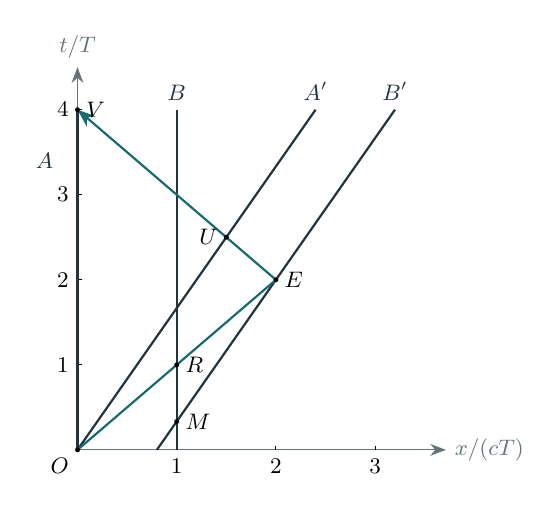
\begin{tikzpicture}[scale=0.9,transform shape]
\draw[axis] (0,0)--(5.2,0) node[right] {$x/(cT)$};\draw[axis] (0,0)--(0,5.4) node[above] {$t/T$};
\foreach \v in {1,2,3}
  \draw ({1.4*\v},.06)--({1.4*\v},0) node[below] {$\v$};
\foreach \v in {1,2,3,4}
  \draw (.065,{1.2*\v})--(0,{1.2*\v}) node[left] {$\v$};
\draw[object] (0,0)--(0,4.8) node[pos=.85,left=6pt] {$A$};\draw[object] (1.4,0)--(1.4,4.8) node[above] {$B$};
\draw[object] (0,0)--(3.36,4.8) node[above] {$A'$};\draw[object] (1.12,0)--(4.48,4.8) node[above] {$B'$};
\draw[motion] (0,0)--(2.8,2.4)--(0,4.8);
\fill (0,0) circle(.035) node[below left] {$O$};\fill (1.4,.4) circle(.035) node[right] {$M$};
\fill (1.4,1.2) circle(.035) node[right] {$R$};\fill (2.8,2.4) circle(.035) node[right] {$E$};
\fill (2.1,3) circle(.035) node[left] {$U$};\fill (0,4.8) circle(.035) node[right] {$V$};\end{tikzpicture}
\figcaption{解图近试.4C\quad $\beta=0.6$的实际事件图：$R$为$B$收光，$E$为$B^\prime$收光回发，$U$为$A^\prime$收回光，$V$为$A$收回光}
\end{minipage}\end{center}


\Needspace{8\baselineskip}

\pdfbookmark[3]{关键洞察}{q4-h5}

\subsection*{关键洞察}

本题远端钟的零点分别对应同一个$M$事件，它在两系中的时间坐标一正一负，因此两尺上远端钟各有不同偏移。标准坐标先保持爱因斯坦同步，实际钟再按零点表读数，使坐标和归零约定的作用清楚分开。

\Needspace{8\baselineskip}

\pdfbookmark[3]{易错点}{q4-h6}

\subsection*{易错点}

$O$与$M$是两个不同事件，各钟在自己的相遇事件归零。$B$读数为$t-t_m$，$B'$为$t'+t_m$；光程计算后还要加对应偏移。原光到$B$与到$B'$在不同位置发生。回光过$A'$后继续到$A$，这一段距离由两者分离程度确定。每段光程使用所选参考系中的静长或收缩长。

\Needspace{8\baselineskip}

\pdfbookmark[3]{课堂讲解建议}{q4-h7}

\subsection*{课堂讲解建议}

从$\beta=0.6$开始，让学生画四条端点世界线、两个归零事件及原光与回光。在每个收光交点旁先写钟名，再写该钟的读数式。用$B'$读1确定$T=3/4$，得到$1/2,3/2,3$后，再归纳一般$\beta$公式。最后讨论低速极限的1、2、2和接近光速时的不同返回等待时间，将代数结果联系到同一时空图。

\Needspace{8\baselineskip}

\pdfbookmark[3]{变式训练}{q4-h8}

\subsection*{变式训练}

\begin{enumerate}
\Needspace{37\baselineskip}
\item \textbf{题设与求解。} 取$\beta=0.6$，求所有尺度与三个钟读数。$\gamma=1.25$、$D=1/2$，故$T=(1+D)/2=3/4$，$t_m=(1-D)/2=1/4$。$B$收到原光时读$T-t_m=1/2$，$A'$收到回光时读$2T=3/2$，$A$最后读$2T/D=3$。图V1在同一时间单位上标出这些读数，每个刻度对应实际钟的指定事件。
\begin{center}\begin{minipage}{.98\linewidth}\centering
\begin{tikzpicture}[scale=0.72,transform shape]
\draw[axis] (0,0)--(6.2,0) node[right] {钟读数};\draw[very thick,color=accent] (0,1.0)--(0.9,1.0);\node[left] at (-.2,1.0) {$B$};\node[right] at (0.9,1.0) {$ 0.5 $};\draw[very thick,color=accent] (0,2.1)--(2.7,2.1);\node[left] at (-.2,2.1) {$A'$};\node[right] at (2.7,2.1) {$ 1.5 $};\draw[very thick,color=accent] (0,3.2)--(5.4,3.2);\node[left] at (-.2,3.2) {$A$};\node[right] at (5.4,3.2) {$ 3 $};\end{tikzpicture}
\figcaption{解图近试.4V1\quad $\beta=0.6$时按指定收光事件比较三只钟读数}
\end{minipage}\end{center}
\Needspace{37\baselineskip}
\item \textbf{题设与求解。} 求低速时三答案的一阶展开。用$(1\pm\beta)^{\pm1/2}$展开，$D=1-\beta+O(\beta^2)$，所以$B$读$1-\beta+O(\beta^2)$、$A'$返回读$2-\beta+O(\beta^2)$，$A$返回读$2+\beta+O(\beta^2)$。两返回读数之差一阶为$2\beta$。解图V2比较一般公式和小速度直线，在$\beta$很小时两者贴近。
\begin{center}\begin{minipage}{.98\linewidth}\centering
\begin{tikzpicture}[scale=0.72,transform shape]
\draw[axis] (0,0)--(6.2,0);\draw[axis] (0,0)--(0,3.4000000000000004);
\draw[thin,color=muted] (0.0000000,0)--(0.0000000,-.07);\node[below] at (0.0000000,-.09) {$0$};
\draw[thin,color=muted] (2.0000000,0)--(2.0000000,-.07);\node[below] at (2.0000000,-.09) {$.1$};
\draw[thin,color=muted] (6.0000000,0)--(6.0000000,-.07);\node[below] at (6.0000000,-.09) {$.3$};
\draw[thin,color=muted] (0,0.0000000)--(-.07,0.0000000);\node[left] at (-.09,0.0000000) {$.7$};
\draw[thin,color=muted] (0,1.0000000)--(-.07,1.0000000);\node[left] at (-.09,1.0000000) {$.8$};
\draw[thin,color=muted] (0,3.0000000)--(-.07,3.0000000);\node[left] at (-.09,3.0000000) {$1$};
\node[below] at (3.0,-.64) {$\beta$};\node[above right] at (0,3.45) {B收光读数};
\draw[traj] plot coordinates {(0.0000000,3.0000000) (0.0300000,2.9850112) (0.0600000,2.9700449) (0.0900000,2.9551008) (0.1200000,2.9401789) (0.1500000,2.9252792) (0.1800000,2.9104014) (0.2100000,2.8955455) (0.2400000,2.8807114) (0.2700000,2.8658991) (0.3000000,2.8511083) (0.3300000,2.8363391) (0.3600000,2.8215912) (0.3900000,2.8068647) (0.4200000,2.7921594) (0.4500000,2.7774752) (0.4800000,2.7628121) (0.5100000,2.7481699) (0.5400000,2.7335485) (0.5700000,2.7189479) (0.6000000,2.7043679) (0.6300000,2.6898085) (0.6600000,2.6752696) (0.6900000,2.6607511) (0.7200000,2.6462528) (0.7500000,2.6317747) (0.7800000,2.6173168) (0.8100000,2.6028788) (0.8400000,2.5884608) (0.8700000,2.5740625) (0.9000000,2.5596841) (0.9300000,2.5453253) (0.9600000,2.5309860) (0.9900000,2.5166663) (1.0200000,2.5023659) (1.0500000,2.4880848) (1.0800000,2.4738229) (1.1100000,2.4595802) (1.1400000,2.4453565) (1.1700000,2.4311517) (1.2000000,2.4169658) (1.2300000,2.4027987) (1.2600000,2.3886503) (1.2900000,2.3745205) (1.3200000,2.3604092) (1.3500000,2.3463164) (1.3800000,2.3322419) (1.4100000,2.3181857) (1.4400000,2.3041477) (1.4700000,2.2901278) (1.5000000,2.2761259) (1.5300000,2.2621420) (1.5600000,2.2481759) (1.5900000,2.2342276) (1.6200000,2.2202970) (1.6500000,2.2063840) (1.6800000,2.1924885) (1.7100000,2.1786105) (1.7400000,2.1647499) (1.7700000,2.1509065) (1.8000000,2.1370804) (1.8300000,2.1232714) (1.8600000,2.1094795) (1.8900000,2.0957045) (1.9200000,2.0819465) (1.9500000,2.0682052) (1.9800000,2.0544807) (2.0100000,2.0407729) (2.0400000,2.0270817) (2.0700000,2.0134069) (2.1000000,1.9997486) (2.1300000,1.9861067) (2.1600000,1.9724810) (2.1900000,1.9588715) (2.2200000,1.9452782) (2.2500000,1.9317009) (2.2800000,1.9181396) (2.3100000,1.9045942) (2.3400000,1.8910646) (2.3700000,1.8775508) (2.4000000,1.8640526) (2.4300000,1.8505701) (2.4600000,1.8371030) (2.4900000,1.8236515) (2.5200000,1.8102153) (2.5500000,1.7967944) (2.5800000,1.7833888) (2.6100000,1.7699983) (2.6400000,1.7566229) (2.6700000,1.7432626) (2.7000000,1.7299172) (2.7300000,1.7165866) (2.7600000,1.7032709) (2.7900000,1.6899699) (2.8200000,1.6766836) (2.8500000,1.6634118) (2.8800000,1.6501546) (2.9100000,1.6369118) (2.9400000,1.6236835) (2.9700000,1.6104694) (3.0000000,1.5972695) (3.0300000,1.5840839) (3.0600000,1.5709123) (3.0900000,1.5577548) (3.1200000,1.5446112) (3.1500000,1.5314815) (3.1800000,1.5183657) (3.2100000,1.5052636) (3.2400000,1.4921752) (3.2700000,1.4791004) (3.3000000,1.4660392) (3.3300000,1.4529915) (3.3600000,1.4399572) (3.3900000,1.4269362) (3.4200000,1.4139285) (3.4500000,1.4009341) (3.4800000,1.3879527) (3.5100000,1.3749845) (3.5400000,1.3620293) (3.5700000,1.3490871) (3.6000000,1.3361577) (3.6300000,1.3232412) (3.6600000,1.3103374) (3.6900000,1.2974463) (3.7200000,1.2845678) (3.7500000,1.2717019) (3.7800000,1.2588485) (3.8100000,1.2460075) (3.8400000,1.2331789) (3.8700000,1.2203626) (3.9000000,1.2075585) (3.9300000,1.1947666) (3.9600000,1.1819868) (3.9900000,1.1692191) (4.0200000,1.1564633) (4.0500000,1.1437194) (4.0800000,1.1309874) (4.1100000,1.1182672) (4.1400000,1.1055588) (4.1700000,1.0928620) (4.2000000,1.0801767) (4.2300000,1.0675031) (4.2600000,1.0548409) (4.2900000,1.0421901) (4.3200000,1.0295507) (4.3500000,1.0169226) (4.3800000,1.0043057) (4.4100000,0.9916999) (4.4400000,0.9791053) (4.4700000,0.9665217) (4.5000000,0.9539491) (4.5300000,0.9413874) (4.5600000,0.9288366) (4.5900000,0.9162966) (4.6200000,0.9037673) (4.6500000,0.8912487) (4.6800000,0.8787407) (4.7100000,0.8662432) (4.7400000,0.8537563) (4.7700000,0.8412798) (4.8000000,0.8288136) (4.8300000,0.8163578) (4.8600000,0.8039122) (4.8900000,0.7914768) (4.9200000,0.7790516) (4.9500000,0.7666364) (4.9800000,0.7542313) (5.0100000,0.7418361) (5.0400000,0.7294508) (5.0700000,0.7170753) (5.1000000,0.7047096) (5.1300000,0.6923536) (5.1600000,0.6800073) (5.1900000,0.6676706) (5.2200000,0.6553434) (5.2500000,0.6430257) (5.2800000,0.6307174) (5.3100000,0.6184185) (5.3400000,0.6061289) (5.3700000,0.5938485) (5.4000000,0.5815773) (5.4300000,0.5693153) (5.4600000,0.5570623) (5.4900000,0.5448184) (5.5200000,0.5325833) (5.5500000,0.5203572) (5.5800000,0.5081400) (5.6100000,0.4959315) (5.6400000,0.4837317) (5.6700000,0.4715406) (5.7000000,0.4593581) (5.7300000,0.4471842) (5.7600000,0.4350187) (5.7900000,0.4228617) (5.8200000,0.4107130) (5.8500000,0.3985727) (5.8800000,0.3864406) (5.9100000,0.3743168) (5.9400000,0.3622011) (5.9700000,0.3500934) (6.0000000,0.3379939)};
\draw[traj] (.1,-1.05)--(.7,-1.05);\node[right] at (.85,-1.05) {完整B钟读数};\draw[dashed,thick,color=warm] plot coordinates {(0.0000000,3.0000000) (0.0300000,2.9850000) (0.0600000,2.9700000) (0.0900000,2.9550000) (0.1200000,2.9400000) (0.1500000,2.9250000) (0.1800000,2.9100000) (0.2100000,2.8950000) (0.2400000,2.8800000) (0.2700000,2.8650000) (0.3000000,2.8500000) (0.3300000,2.8350000) (0.3600000,2.8200000) (0.3900000,2.8050000) (0.4200000,2.7900000) (0.4500000,2.7750000) (0.4800000,2.7600000) (0.5100000,2.7450000) (0.5400000,2.7300000) (0.5700000,2.7150000) (0.6000000,2.7000000) (0.6300000,2.6850000) (0.6600000,2.6700000) (0.6900000,2.6550000) (0.7200000,2.6400000) (0.7500000,2.6250000) (0.7800000,2.6100000) (0.8100000,2.5950000) (0.8400000,2.5800000) (0.8700000,2.5650000) (0.9000000,2.5500000) (0.9300000,2.5350000) (0.9600000,2.5200000) (0.9900000,2.5050000) (1.0200000,2.4900000) (1.0500000,2.4750000) (1.0800000,2.4600000) (1.1100000,2.4450000) (1.1400000,2.4300000) (1.1700000,2.4150000) (1.2000000,2.4000000) (1.2300000,2.3850000) (1.2600000,2.3700000) (1.2900000,2.3550000) (1.3200000,2.3400000) (1.3500000,2.3250000) (1.3800000,2.3100000) (1.4100000,2.2950000) (1.4400000,2.2800000) (1.4700000,2.2650000) (1.5000000,2.2500000) (1.5300000,2.2350000) (1.5600000,2.2200000) (1.5900000,2.2050000) (1.6200000,2.1900000) (1.6500000,2.1750000) (1.6800000,2.1600000) (1.7100000,2.1450000) (1.7400000,2.1300000) (1.7700000,2.1150000) (1.8000000,2.1000000) (1.8300000,2.0850000) (1.8600000,2.0700000) (1.8900000,2.0550000) (1.9200000,2.0400000) (1.9500000,2.0250000) (1.9800000,2.0100000) (2.0100000,1.9950000) (2.0400000,1.9800000) (2.0700000,1.9650000) (2.1000000,1.9500000) (2.1300000,1.9350000) (2.1600000,1.9200000) (2.1900000,1.9050000) (2.2200000,1.8900000) (2.2500000,1.8750000) (2.2800000,1.8600000) (2.3100000,1.8450000) (2.3400000,1.8300000) (2.3700000,1.8150000) (2.4000000,1.8000000) (2.4300000,1.7850000) (2.4600000,1.7700000) (2.4900000,1.7550000) (2.5200000,1.7400000) (2.5500000,1.7250000) (2.5800000,1.7100000) (2.6100000,1.6950000) (2.6400000,1.6800000) (2.6700000,1.6650000) (2.7000000,1.6500000) (2.7300000,1.6350000) (2.7600000,1.6200000) (2.7900000,1.6050000) (2.8200000,1.5900000) (2.8500000,1.5750000) (2.8800000,1.5600000) (2.9100000,1.5450000) (2.9400000,1.5300000) (2.9700000,1.5150000) (3.0000000,1.5000000) (3.0300000,1.4850000) (3.0600000,1.4700000) (3.0900000,1.4550000) (3.1200000,1.4400000) (3.1500000,1.4250000) (3.1800000,1.4100000) (3.2100000,1.3950000) (3.2400000,1.3800000) (3.2700000,1.3650000) (3.3000000,1.3500000) (3.3300000,1.3350000) (3.3600000,1.3200000) (3.3900000,1.3050000) (3.4200000,1.2900000) (3.4500000,1.2750000) (3.4800000,1.2600000) (3.5100000,1.2450000) (3.5400000,1.2300000) (3.5700000,1.2150000) (3.6000000,1.2000000) (3.6300000,1.1850000) (3.6600000,1.1700000) (3.6900000,1.1550000) (3.7200000,1.1400000) (3.7500000,1.1250000) (3.7800000,1.1100000) (3.8100000,1.0950000) (3.8400000,1.0800000) (3.8700000,1.0650000) (3.9000000,1.0500000) (3.9300000,1.0350000) (3.9600000,1.0200000) (3.9900000,1.0050000) (4.0200000,0.9900000) (4.0500000,0.9750000) (4.0800000,0.9600000) (4.1100000,0.9450000) (4.1400000,0.9300000) (4.1700000,0.9150000) (4.2000000,0.9000000) (4.2300000,0.8850000) (4.2600000,0.8700000) (4.2900000,0.8550000) (4.3200000,0.8400000) (4.3500000,0.8250000) (4.3800000,0.8100000) (4.4100000,0.7950000) (4.4400000,0.7800000) (4.4700000,0.7650000) (4.5000000,0.7500000) (4.5300000,0.7350000) (4.5600000,0.7200000) (4.5900000,0.7050000) (4.6200000,0.6900000) (4.6500000,0.6750000) (4.6800000,0.6600000) (4.7100000,0.6450000) (4.7400000,0.6300000) (4.7700000,0.6150000) (4.8000000,0.6000000) (4.8300000,0.5850000) (4.8600000,0.5700000) (4.8900000,0.5550000) (4.9200000,0.5400000) (4.9500000,0.5250000) (4.9800000,0.5100000) (5.0100000,0.4950000) (5.0400000,0.4800000) (5.0700000,0.4650000) (5.1000000,0.4500000) (5.1300000,0.4350000) (5.1600000,0.4200000) (5.1900000,0.4050000) (5.2200000,0.3900000) (5.2500000,0.3750000) (5.2800000,0.3600000) (5.3100000,0.3450000) (5.3400000,0.3300000) (5.3700000,0.3150000) (5.4000000,0.3000000) (5.4300000,0.2850000) (5.4600000,0.2700000) (5.4900000,0.2550000) (5.5200000,0.2400000) (5.5500000,0.2250000) (5.5800000,0.2100000) (5.6100000,0.1950000) (5.6400000,0.1800000) (5.6700000,0.1650000) (5.7000000,0.1500000) (5.7300000,0.1350000) (5.7600000,0.1200000) (5.7900000,0.1050000) (5.8200000,0.0900000) (5.8500000,0.0750000) (5.8800000,0.0600000) (5.9100000,0.0450000) (5.9400000,0.0300000) (5.9700000,0.0150000) (6.0000000,0.0000000)};
\draw[dashed,thick,color=warm] (.1,-1.48)--(.7,-1.48);\node[right] at (.85,-1.48) {一阶低速式};\end{tikzpicture}
\figcaption{解图近试.4V2\quad 低速读数的一阶项随相对速度线性下降}
\end{minipage}\end{center}
\Needspace{37\baselineskip}
\item \textbf{题设与求解。} 求$\beta\to1^-$时的读数变化。$D=\sqrt{(1-\beta)/(1+\beta)}\to0$，从而$B$读数趋0、$A'$返回读数趋1、$A$返回读数$1+1/D$发散。单位由远端$B'$接收时读1确定，此时$T=(1+D)/2\to1/2$，$t_m\to1/2$；$B$的收光时间和其归零时间趋近，而回光到静止$A$的等待变长。图V3分别画这三种变化。
\begin{center}\begin{minipage}{.98\linewidth}\centering
\begin{tikzpicture}[scale=0.72,transform shape]
\draw[axis] (0,0)--(6.2,0);\draw[axis] (0,0)--(0,3.4000000000000004);
\draw[thin,color=muted] (0.0000000,0)--(0.0000000,-.07);\node[below] at (0.0000000,-.09) {$.1$};
\draw[thin,color=muted] (3.3707865,0)--(3.3707865,-.07);\node[below] at (3.3707865,-.09) {$.6$};
\draw[thin,color=muted] (5.3932584,0)--(5.3932584,-.07);\node[below] at (5.3932584,-.09) {$.9$};
\draw[thin,color=muted] (6.0000000,0)--(6.0000000,-.07);\node[below] at (6.0000000,-.09) {$.99$};
\draw[thin,color=muted] (0,0.0000000)--(-.07,0.0000000);\node[left] at (-.09,0.0000000) {$0$};
\draw[thin,color=muted] (0,0.2000000)--(-.07,0.2000000);\node[left] at (-.09,0.2000000) {$1$};
\draw[thin,color=muted] (0,1.0000000)--(-.07,1.0000000);\node[left] at (-.09,1.0000000) {$5$};
\draw[thin,color=muted] (0,3.0000000)--(-.07,3.0000000);\node[left] at (-.09,3.0000000) {$15$};
\node[below] at (3.0,-.64) {$\beta$};\node[above right] at (0,3.45) {钟读数};
\draw[traj] plot coordinates {(0.0000000,0.1809068) (0.0200000,0.1803653) (0.0400000,0.1798252) (0.0600000,0.1792863) (0.0800000,0.1787486) (0.1000000,0.1782122) (0.1200000,0.1776771) (0.1400000,0.1771432) (0.1600000,0.1766105) (0.1800000,0.1760790) (0.2000000,0.1755487) (0.2200000,0.1750196) (0.2400000,0.1744917) (0.2600000,0.1739649) (0.2800000,0.1734393) (0.3000000,0.1729148) (0.3200000,0.1723914) (0.3400000,0.1718692) (0.3600000,0.1713480) (0.3800000,0.1708280) (0.4000000,0.1703091) (0.4200000,0.1697912) (0.4400000,0.1692744) (0.4600000,0.1687586) (0.4800000,0.1682439) (0.5000000,0.1677302) (0.5200000,0.1672176) (0.5400000,0.1667059) (0.5600000,0.1661953) (0.5800000,0.1656856) (0.6000000,0.1651770) (0.6200000,0.1646693) (0.6400000,0.1641625) (0.6600000,0.1636568) (0.6800000,0.1631519) (0.7000000,0.1626480) (0.7200000,0.1621451) (0.7400000,0.1616430) (0.7600000,0.1611418) (0.7800000,0.1606416) (0.8000000,0.1601422) (0.8200000,0.1596437) (0.8400000,0.1591460) (0.8600000,0.1586492) (0.8800000,0.1581533) (0.9000000,0.1576582) (0.9200000,0.1571639) (0.9400000,0.1566704) (0.9600000,0.1561778) (0.9800000,0.1556859) (1.0000000,0.1551949) (1.0200000,0.1547046) (1.0400000,0.1542151) (1.0600000,0.1537263) (1.0800000,0.1532383) (1.1000000,0.1527511) (1.1200000,0.1522646) (1.1400000,0.1517788) (1.1600000,0.1512937) (1.1800000,0.1508093) (1.2000000,0.1503257) (1.2200000,0.1498427) (1.2400000,0.1493604) (1.2600000,0.1488788) (1.2800000,0.1483978) (1.3000000,0.1479175) (1.3200000,0.1474379) (1.3400000,0.1469588) (1.3600000,0.1464804) (1.3800000,0.1460027) (1.4000000,0.1455255) (1.4200000,0.1450489) (1.4400000,0.1445730) (1.4600000,0.1440976) (1.4800000,0.1436228) (1.5000000,0.1431485) (1.5200000,0.1426748) (1.5400000,0.1422017) (1.5600000,0.1417291) (1.5800000,0.1412570) (1.6000000,0.1407854) (1.6200000,0.1403144) (1.6400000,0.1398439) (1.6600000,0.1393738) (1.6800000,0.1389043) (1.7000000,0.1384352) (1.7200000,0.1379666) (1.7400000,0.1374985) (1.7600000,0.1370308) (1.7800000,0.1365635) (1.8000000,0.1360967) (1.8200000,0.1356303) (1.8400000,0.1351643) (1.8600000,0.1346988) (1.8800000,0.1342336) (1.9000000,0.1337688) (1.9200000,0.1333044) (1.9400000,0.1328404) (1.9600000,0.1323768) (1.9800000,0.1319135) (2.0000000,0.1314505) (2.0200000,0.1309879) (2.0400000,0.1305256) (2.0600000,0.1300636) (2.0800000,0.1296020) (2.1000000,0.1291406) (2.1200000,0.1286795) (2.1400000,0.1282187) (2.1600000,0.1277582) (2.1800000,0.1272980) (2.2000000,0.1268380) (2.2200000,0.1263782) (2.2400000,0.1259187) (2.2600000,0.1254594) (2.2800000,0.1250003) (2.3000000,0.1245415) (2.3200000,0.1240828) (2.3400000,0.1236243) (2.3600000,0.1231661) (2.3800000,0.1227079) (2.4000000,0.1222500) (2.4200000,0.1217922) (2.4400000,0.1213345) (2.4600000,0.1208769) (2.4800000,0.1204195) (2.5000000,0.1199622) (2.5200000,0.1195050) (2.5400000,0.1190479) (2.5600000,0.1185909) (2.5800000,0.1181339) (2.6000000,0.1176770) (2.6200000,0.1172202) (2.6400000,0.1167634) (2.6600000,0.1163066) (2.6800000,0.1158498) (2.7000000,0.1153931) (2.7200000,0.1149363) (2.7400000,0.1144796) (2.7600000,0.1140228) (2.7800000,0.1135660) (2.8000000,0.1131091) (2.8200000,0.1126522) (2.8400000,0.1121952) (2.8600000,0.1117381) (2.8800000,0.1112809) (2.9000000,0.1108237) (2.9200000,0.1103663) (2.9400000,0.1099088) (2.9600000,0.1094512) (2.9800000,0.1089934) (3.0000000,0.1085354) (3.0200000,0.1080773) (3.0400000,0.1076190) (3.0600000,0.1071605) (3.0800000,0.1067017) (3.1000000,0.1062428) (3.1200000,0.1057836) (3.1400000,0.1053242) (3.1600000,0.1048645) (3.1800000,0.1044045) (3.2000000,0.1039442) (3.2200000,0.1034837) (3.2400000,0.1030228) (3.2600000,0.1025615) (3.2800000,0.1021000) (3.3000000,0.1016380) (3.3200000,0.1011757) (3.3400000,0.1007130) (3.3600000,0.1002499) (3.3800000,0.0997864) (3.4000000,0.0993225) (3.4200000,0.0988580) (3.4400000,0.0983932) (3.4600000,0.0979278) (3.4800000,0.0974619) (3.5000000,0.0969955) (3.5200000,0.0965286) (3.5400000,0.0960611) (3.5600000,0.0955931) (3.5800000,0.0951244) (3.6000000,0.0946552) (3.6200000,0.0941853) (3.6400000,0.0937148) (3.6600000,0.0932437) (3.6800000,0.0927718) (3.7000000,0.0922993) (3.7200000,0.0918260) (3.7400000,0.0913520) (3.7600000,0.0908772) (3.7800000,0.0904016) (3.8000000,0.0899253) (3.8200000,0.0894481) (3.8400000,0.0889700) (3.8600000,0.0884911) (3.8800000,0.0880113) (3.9000000,0.0875306) (3.9200000,0.0870489) (3.9400000,0.0865663) (3.9600000,0.0860826) (3.9800000,0.0855980) (4.0000000,0.0851122) (4.0200000,0.0846255) (4.0400000,0.0841376) (4.0600000,0.0836486) (4.0800000,0.0831584) (4.1000000,0.0826670) (4.1200000,0.0821744) (4.1400000,0.0816806) (4.1600000,0.0811855) (4.1800000,0.0806891) (4.2000000,0.0801913) (4.2200000,0.0796921) (4.2400000,0.0791916) (4.2600000,0.0786895) (4.2800000,0.0781860) (4.3000000,0.0776810) (4.3200000,0.0771744) (4.3400000,0.0766661) (4.3600000,0.0761563) (4.3800000,0.0756447) (4.4000000,0.0751314) (4.4200000,0.0746164) (4.4400000,0.0740995) (4.4600000,0.0735807) (4.4800000,0.0730600) (4.5000000,0.0725374) (4.5200000,0.0720127) (4.5400000,0.0714859) (4.5600000,0.0709570) (4.5800000,0.0704260) (4.6000000,0.0698926) (4.6200000,0.0693570) (4.6400000,0.0688190) (4.6600000,0.0682786) (4.6800000,0.0677356) (4.7000000,0.0671901) (4.7200000,0.0666420) (4.7400000,0.0660911) (4.7600000,0.0655374) (4.7800000,0.0649809) (4.8000000,0.0644214) (4.8200000,0.0638588) (4.8400000,0.0632931) (4.8600000,0.0627241) (4.8800000,0.0621519) (4.9000000,0.0615762) (4.9200000,0.0609969) (4.9400000,0.0604140) (4.9600000,0.0598274) (4.9800000,0.0592368) (5.0000000,0.0586423) (5.0200000,0.0580435) (5.0400000,0.0574405) (5.0600000,0.0568331) (5.0800000,0.0562211) (5.1000000,0.0556043) (5.1200000,0.0549826) (5.1400000,0.0543558) (5.1600000,0.0537238) (5.1800000,0.0530862) (5.2000000,0.0524430) (5.2200000,0.0517938) (5.2400000,0.0511385) (5.2600000,0.0504768) (5.2800000,0.0498085) (5.3000000,0.0491332) (5.3200000,0.0484506) (5.3400000,0.0477605) (5.3600000,0.0470624) (5.3800000,0.0463561) (5.4000000,0.0456411) (5.4200000,0.0449171) (5.4400000,0.0441834) (5.4600000,0.0434397) (5.4800000,0.0426854) (5.5000000,0.0419200) (5.5200000,0.0411427) (5.5400000,0.0403530) (5.5600000,0.0395500) (5.5800000,0.0387328) (5.6000000,0.0379007) (5.6200000,0.0370525) (5.6400000,0.0361872) (5.6600000,0.0353033) (5.6800000,0.0343996) (5.7000000,0.0334744) (5.7200000,0.0325258) (5.7400000,0.0315517) (5.7600000,0.0305496) (5.7800000,0.0295168) (5.8000000,0.0284497) (5.8200000,0.0273445) (5.8400000,0.0261962) (5.8600000,0.0249989) (5.8800000,0.0237453) (5.9000000,0.0224257) (5.9200000,0.0210278) (5.9400000,0.0195347) (5.9600000,0.0179228) (5.9800000,0.0161563) (6.0000000,0.0141776)};
\draw[traj] (.1,-1.05)--(.7,-1.05);\node[right] at (.85,-1.05) {B原光};\draw[dashed,thick,color=warm] plot coordinates {(0.0000000,0.3809068) (0.0200000,0.3803653) (0.0400000,0.3798252) (0.0600000,0.3792863) (0.0800000,0.3787486) (0.1000000,0.3782122) (0.1200000,0.3776771) (0.1400000,0.3771432) (0.1600000,0.3766105) (0.1800000,0.3760790) (0.2000000,0.3755487) (0.2200000,0.3750196) (0.2400000,0.3744917) (0.2600000,0.3739649) (0.2800000,0.3734393) (0.3000000,0.3729148) (0.3200000,0.3723914) (0.3400000,0.3718692) (0.3600000,0.3713480) (0.3800000,0.3708280) (0.4000000,0.3703091) (0.4200000,0.3697912) (0.4400000,0.3692744) (0.4600000,0.3687586) (0.4800000,0.3682439) (0.5000000,0.3677302) (0.5200000,0.3672176) (0.5400000,0.3667059) (0.5600000,0.3661953) (0.5800000,0.3656856) (0.6000000,0.3651770) (0.6200000,0.3646693) (0.6400000,0.3641625) (0.6600000,0.3636568) (0.6800000,0.3631519) (0.7000000,0.3626480) (0.7200000,0.3621451) (0.7400000,0.3616430) (0.7600000,0.3611418) (0.7800000,0.3606416) (0.8000000,0.3601422) (0.8200000,0.3596437) (0.8400000,0.3591460) (0.8600000,0.3586492) (0.8800000,0.3581533) (0.9000000,0.3576582) (0.9200000,0.3571639) (0.9400000,0.3566704) (0.9600000,0.3561778) (0.9800000,0.3556859) (1.0000000,0.3551949) (1.0200000,0.3547046) (1.0400000,0.3542151) (1.0600000,0.3537263) (1.0800000,0.3532383) (1.1000000,0.3527511) (1.1200000,0.3522646) (1.1400000,0.3517788) (1.1600000,0.3512937) (1.1800000,0.3508093) (1.2000000,0.3503257) (1.2200000,0.3498427) (1.2400000,0.3493604) (1.2600000,0.3488788) (1.2800000,0.3483978) (1.3000000,0.3479175) (1.3200000,0.3474379) (1.3400000,0.3469588) (1.3600000,0.3464804) (1.3800000,0.3460027) (1.4000000,0.3455255) (1.4200000,0.3450489) (1.4400000,0.3445730) (1.4600000,0.3440976) (1.4800000,0.3436228) (1.5000000,0.3431485) (1.5200000,0.3426748) (1.5400000,0.3422017) (1.5600000,0.3417291) (1.5800000,0.3412570) (1.6000000,0.3407854) (1.6200000,0.3403144) (1.6400000,0.3398439) (1.6600000,0.3393738) (1.6800000,0.3389043) (1.7000000,0.3384352) (1.7200000,0.3379666) (1.7400000,0.3374985) (1.7600000,0.3370308) (1.7800000,0.3365635) (1.8000000,0.3360967) (1.8200000,0.3356303) (1.8400000,0.3351643) (1.8600000,0.3346988) (1.8800000,0.3342336) (1.9000000,0.3337688) (1.9200000,0.3333044) (1.9400000,0.3328404) (1.9600000,0.3323768) (1.9800000,0.3319135) (2.0000000,0.3314505) (2.0200000,0.3309879) (2.0400000,0.3305256) (2.0600000,0.3300636) (2.0800000,0.3296020) (2.1000000,0.3291406) (2.1200000,0.3286795) (2.1400000,0.3282187) (2.1600000,0.3277582) (2.1800000,0.3272980) (2.2000000,0.3268380) (2.2200000,0.3263782) (2.2400000,0.3259187) (2.2600000,0.3254594) (2.2800000,0.3250003) (2.3000000,0.3245415) (2.3200000,0.3240828) (2.3400000,0.3236243) (2.3600000,0.3231661) (2.3800000,0.3227079) (2.4000000,0.3222500) (2.4200000,0.3217922) (2.4400000,0.3213345) (2.4600000,0.3208769) (2.4800000,0.3204195) (2.5000000,0.3199622) (2.5200000,0.3195050) (2.5400000,0.3190479) (2.5600000,0.3185909) (2.5800000,0.3181339) (2.6000000,0.3176770) (2.6200000,0.3172202) (2.6400000,0.3167634) (2.6600000,0.3163066) (2.6800000,0.3158498) (2.7000000,0.3153931) (2.7200000,0.3149363) (2.7400000,0.3144796) (2.7600000,0.3140228) (2.7800000,0.3135660) (2.8000000,0.3131091) (2.8200000,0.3126522) (2.8400000,0.3121952) (2.8600000,0.3117381) (2.8800000,0.3112809) (2.9000000,0.3108237) (2.9200000,0.3103663) (2.9400000,0.3099088) (2.9600000,0.3094512) (2.9800000,0.3089934) (3.0000000,0.3085354) (3.0200000,0.3080773) (3.0400000,0.3076190) (3.0600000,0.3071605) (3.0800000,0.3067017) (3.1000000,0.3062428) (3.1200000,0.3057836) (3.1400000,0.3053242) (3.1600000,0.3048645) (3.1800000,0.3044045) (3.2000000,0.3039442) (3.2200000,0.3034837) (3.2400000,0.3030228) (3.2600000,0.3025615) (3.2800000,0.3021000) (3.3000000,0.3016380) (3.3200000,0.3011757) (3.3400000,0.3007130) (3.3600000,0.3002499) (3.3800000,0.2997864) (3.4000000,0.2993225) (3.4200000,0.2988580) (3.4400000,0.2983932) (3.4600000,0.2979278) (3.4800000,0.2974619) (3.5000000,0.2969955) (3.5200000,0.2965286) (3.5400000,0.2960611) (3.5600000,0.2955931) (3.5800000,0.2951244) (3.6000000,0.2946552) (3.6200000,0.2941853) (3.6400000,0.2937148) (3.6600000,0.2932437) (3.6800000,0.2927718) (3.7000000,0.2922993) (3.7200000,0.2918260) (3.7400000,0.2913520) (3.7600000,0.2908772) (3.7800000,0.2904016) (3.8000000,0.2899253) (3.8200000,0.2894481) (3.8400000,0.2889700) (3.8600000,0.2884911) (3.8800000,0.2880113) (3.9000000,0.2875306) (3.9200000,0.2870489) (3.9400000,0.2865663) (3.9600000,0.2860826) (3.9800000,0.2855980) (4.0000000,0.2851122) (4.0200000,0.2846255) (4.0400000,0.2841376) (4.0600000,0.2836486) (4.0800000,0.2831584) (4.1000000,0.2826670) (4.1200000,0.2821744) (4.1400000,0.2816806) (4.1600000,0.2811855) (4.1800000,0.2806891) (4.2000000,0.2801913) (4.2200000,0.2796921) (4.2400000,0.2791916) (4.2600000,0.2786895) (4.2800000,0.2781860) (4.3000000,0.2776810) (4.3200000,0.2771744) (4.3400000,0.2766661) (4.3600000,0.2761563) (4.3800000,0.2756447) (4.4000000,0.2751314) (4.4200000,0.2746164) (4.4400000,0.2740995) (4.4600000,0.2735807) (4.4800000,0.2730600) (4.5000000,0.2725374) (4.5200000,0.2720127) (4.5400000,0.2714859) (4.5600000,0.2709570) (4.5800000,0.2704260) (4.6000000,0.2698926) (4.6200000,0.2693570) (4.6400000,0.2688190) (4.6600000,0.2682786) (4.6800000,0.2677356) (4.7000000,0.2671901) (4.7200000,0.2666420) (4.7400000,0.2660911) (4.7600000,0.2655374) (4.7800000,0.2649809) (4.8000000,0.2644214) (4.8200000,0.2638588) (4.8400000,0.2632931) (4.8600000,0.2627241) (4.8800000,0.2621519) (4.9000000,0.2615762) (4.9200000,0.2609969) (4.9400000,0.2604140) (4.9600000,0.2598274) (4.9800000,0.2592368) (5.0000000,0.2586423) (5.0200000,0.2580435) (5.0400000,0.2574405) (5.0600000,0.2568331) (5.0800000,0.2562211) (5.1000000,0.2556043) (5.1200000,0.2549826) (5.1400000,0.2543558) (5.1600000,0.2537238) (5.1800000,0.2530862) (5.2000000,0.2524430) (5.2200000,0.2517938) (5.2400000,0.2511385) (5.2600000,0.2504768) (5.2800000,0.2498085) (5.3000000,0.2491332) (5.3200000,0.2484506) (5.3400000,0.2477605) (5.3600000,0.2470624) (5.3800000,0.2463561) (5.4000000,0.2456411) (5.4200000,0.2449171) (5.4400000,0.2441834) (5.4600000,0.2434397) (5.4800000,0.2426854) (5.5000000,0.2419200) (5.5200000,0.2411427) (5.5400000,0.2403530) (5.5600000,0.2395500) (5.5800000,0.2387328) (5.6000000,0.2379007) (5.6200000,0.2370525) (5.6400000,0.2361872) (5.6600000,0.2353033) (5.6800000,0.2343996) (5.7000000,0.2334744) (5.7200000,0.2325258) (5.7400000,0.2315517) (5.7600000,0.2305496) (5.7800000,0.2295168) (5.8000000,0.2284497) (5.8200000,0.2273445) (5.8400000,0.2261962) (5.8600000,0.2249989) (5.8800000,0.2237453) (5.9000000,0.2224257) (5.9200000,0.2210278) (5.9400000,0.2195347) (5.9600000,0.2179228) (5.9800000,0.2161563) (6.0000000,0.2141776)};
\draw[dashed,thick,color=warm] (.1,-1.48)--(.7,-1.48);\node[right] at (.85,-1.48) {$A^{\prime}$回光};\draw[dotted,thick,color=muted] plot coordinates {(0.0000000,0.4211083) (0.0200000,0.4217721) (0.0400000,0.4224383) (0.0600000,0.4231069) (0.0800000,0.4237779) (0.1000000,0.4244515) (0.1200000,0.4251275) (0.1400000,0.4258060) (0.1600000,0.4264871) (0.1800000,0.4271708) (0.2000000,0.4278570) (0.2200000,0.4285458) (0.2400000,0.4292373) (0.2600000,0.4299315) (0.2800000,0.4306283) (0.3000000,0.4313278) (0.3200000,0.4320301) (0.3400000,0.4327352) (0.3600000,0.4334430) (0.3800000,0.4341536) (0.4000000,0.4348671) (0.4200000,0.4355835) (0.4400000,0.4363028) (0.4600000,0.4370249) (0.4800000,0.4377501) (0.5000000,0.4384782) (0.5200000,0.4392093) (0.5400000,0.4399435) (0.5600000,0.4406807) (0.5800000,0.4414210) (0.6000000,0.4421645) (0.6200000,0.4429111) (0.6400000,0.4436609) (0.6600000,0.4444140) (0.6800000,0.4451702) (0.7000000,0.4459298) (0.7200000,0.4466927) (0.7400000,0.4474589) (0.7600000,0.4482285) (0.7800000,0.4490016) (0.8000000,0.4497781) (0.8200000,0.4505580) (0.8400000,0.4513415) (0.8600000,0.4521286) (0.8800000,0.4529192) (0.9000000,0.4537135) (0.9200000,0.4545114) (0.9400000,0.4553130) (0.9600000,0.4561184) (0.9800000,0.4569275) (1.0000000,0.4577405) (1.0200000,0.4585573) (1.0400000,0.4593780) (1.0600000,0.4602027) (1.0800000,0.4610313) (1.1000000,0.4618639) (1.1200000,0.4627006) (1.1400000,0.4635415) (1.1600000,0.4643864) (1.1800000,0.4652356) (1.2000000,0.4660889) (1.2200000,0.4669466) (1.2400000,0.4678086) (1.2600000,0.4686750) (1.2800000,0.4695457) (1.3000000,0.4704210) (1.3200000,0.4713007) (1.3400000,0.4721851) (1.3600000,0.4730740) (1.3800000,0.4739676) (1.4000000,0.4748659) (1.4200000,0.4757690) (1.4400000,0.4766769) (1.4600000,0.4775897) (1.4800000,0.4785074) (1.5000000,0.4794301) (1.5200000,0.4803578) (1.5400000,0.4812907) (1.5600000,0.4822286) (1.5800000,0.4831718) (1.6000000,0.4841203) (1.6200000,0.4850741) (1.6400000,0.4860333) (1.6600000,0.4869979) (1.6800000,0.4879681) (1.7000000,0.4889439) (1.7200000,0.4899253) (1.7400000,0.4909124) (1.7600000,0.4919053) (1.7800000,0.4929040) (1.8000000,0.4939087) (1.8200000,0.4949193) (1.8400000,0.4959360) (1.8600000,0.4969589) (1.8800000,0.4979880) (1.9000000,0.4990233) (1.9200000,0.5000650) (1.9400000,0.5011132) (1.9600000,0.5021678) (1.9800000,0.5032291) (2.0000000,0.5042970) (2.0200000,0.5053717) (2.0400000,0.5064533) (2.0600000,0.5075418) (2.0800000,0.5086373) (2.1000000,0.5097399) (2.1200000,0.5108498) (2.1400000,0.5119669) (2.1600000,0.5130914) (2.1800000,0.5142234) (2.2000000,0.5153630) (2.2200000,0.5165102) (2.2400000,0.5176653) (2.2600000,0.5188282) (2.2800000,0.5199991) (2.3000000,0.5211781) (2.3200000,0.5223653) (2.3400000,0.5235609) (2.3600000,0.5247648) (2.3800000,0.5259773) (2.4000000,0.5271984) (2.4200000,0.5284284) (2.4400000,0.5296672) (2.4600000,0.5309150) (2.4800000,0.5321720) (2.5000000,0.5334383) (2.5200000,0.5347140) (2.5400000,0.5359992) (2.5600000,0.5372941) (2.5800000,0.5385988) (2.6000000,0.5399135) (2.6200000,0.5412382) (2.6400000,0.5425732) (2.6600000,0.5439186) (2.6800000,0.5452746) (2.7000000,0.5466413) (2.7200000,0.5480188) (2.7400000,0.5494074) (2.7600000,0.5508071) (2.7800000,0.5522182) (2.8000000,0.5536409) (2.8200000,0.5550753) (2.8400000,0.5565216) (2.8600000,0.5579800) (2.8800000,0.5594506) (2.9000000,0.5609337) (2.9200000,0.5624295) (2.9400000,0.5639381) (2.9600000,0.5654598) (2.9800000,0.5669948) (3.0000000,0.5685433) (3.0200000,0.5701055) (3.0400000,0.5716817) (3.0600000,0.5732720) (3.0800000,0.5748767) (3.1000000,0.5764961) (3.1200000,0.5781304) (3.1400000,0.5797799) (3.1600000,0.5814447) (3.1800000,0.5831253) (3.2000000,0.5848217) (3.2200000,0.5865345) (3.2400000,0.5882637) (3.2600000,0.5900097) (3.2800000,0.5917729) (3.3000000,0.5935534) (3.3200000,0.5953517) (3.3400000,0.5971680) (3.3600000,0.5990027) (3.3800000,0.6008562) (3.4000000,0.6027287) (3.4200000,0.6046206) (3.4400000,0.6065324) (3.4600000,0.6084643) (3.4800000,0.6104167) (3.5000000,0.6123902) (3.5200000,0.6143850) (3.5400000,0.6164015) (3.5600000,0.6184403) (3.5800000,0.6205018) (3.6000000,0.6225864) (3.6200000,0.6246945) (3.6400000,0.6268268) (3.6600000,0.6289835) (3.6800000,0.6311654) (3.7000000,0.6333729) (3.7200000,0.6356065) (3.7400000,0.6378668) (3.7600000,0.6401544) (3.7800000,0.6424698) (3.8000000,0.6448137) (3.8200000,0.6471868) (3.8400000,0.6495895) (3.8600000,0.6520227) (3.8800000,0.6544870) (3.9000000,0.6569831) (3.9200000,0.6595118) (3.9400000,0.6620738) (3.9600000,0.6646699) (3.9800000,0.6673009) (4.0000000,0.6699676) (4.0200000,0.6726710) (4.0400000,0.6754118) (4.0600000,0.6781911) (4.0800000,0.6810098) (4.1000000,0.6838689) (4.1200000,0.6867693) (4.1400000,0.6897123) (4.1600000,0.6926988) (4.1800000,0.6957301) (4.2000000,0.6988072) (4.2200000,0.7019316) (4.2400000,0.7051043) (4.2600000,0.7083268) (4.2800000,0.7116004) (4.3000000,0.7149266) (4.3200000,0.7183068) (4.3400000,0.7217427) (4.3600000,0.7252358) (4.3800000,0.7287877) (4.4000000,0.7324004) (4.4200000,0.7360755) (4.4400000,0.7398149) (4.4600000,0.7436208) (4.4800000,0.7474951) (4.5000000,0.7514400) (4.5200000,0.7554577) (4.5400000,0.7595507) (4.5600000,0.7637213) (4.5800000,0.7679723) (4.6000000,0.7723063) (4.6200000,0.7767261) (4.6400000,0.7812347) (4.6600000,0.7858352) (4.6800000,0.7905310) (4.7000000,0.7953255) (4.7200000,0.8002223) (4.7400000,0.8052253) (4.7600000,0.8103383) (4.7800000,0.8155658) (4.8000000,0.8209122) (4.8200000,0.8263821) (4.8400000,0.8319806) (4.8600000,0.8377130) (4.8800000,0.8435848) (4.9000000,0.8496019) (4.9200000,0.8557707) (4.9400000,0.8620978) (4.9600000,0.8685903) (4.9800000,0.8752557) (5.0000000,0.8821020) (5.0200000,0.8891378) (5.0400000,0.8963723) (5.0600000,0.9038152) (5.0800000,0.9114769) (5.1000000,0.9193687) (5.1200000,0.9275026) (5.1400000,0.9358914) (5.1600000,0.9445493) (5.1800000,0.9534911) (5.2000000,0.9627330) (5.2200000,0.9722927) (5.2400000,0.9821890) (5.2600000,0.9924427) (5.2800000,1.0030763) (5.3000000,1.0141141) (5.3200000,1.0255831) (5.3400000,1.0375125) (5.3600000,1.0499346) (5.3800000,1.0628848) (5.4000000,1.0764022) (5.4200000,1.0905302) (5.4400000,1.1053170) (5.4600000,1.1208161) (5.4800000,1.1370876) (5.5000000,1.1541986) (5.5200000,1.1722251) (5.5400000,1.1912528) (5.5600000,1.2113790) (5.5800000,1.2327152) (5.6000000,1.2553891) (5.6200000,1.2795482) (5.6400000,1.3053640) (5.6600000,1.3330370) (5.6800000,1.3628032) (5.7000000,1.3949435) (5.7200000,1.4297940) (5.7400000,1.4677619) (5.7600000,1.5093456) (5.7800000,1.5551627) (5.8000000,1.6059896) (5.8200000,1.6628180) (5.8400000,1.7269386) (5.8600000,1.8000677) (5.8800000,1.8845468) (5.9000000,1.9836694) (5.9200000,2.1022451) (5.9400000,2.2476338) (5.9600000,2.4317976) (5.9800000,2.6758162) (6.0000000,3.0213472)};
\draw[dotted,thick,color=muted] (.1,-1.9100000000000001)--(.7,-1.9100000000000001);\node[right] at (.85,-1.9100000000000001) {A回光};\end{tikzpicture}
\figcaption{解图近试.4V3\quad 接近光速时三个不同事件的归一化读数呈不同极限}
\end{minipage}\end{center}
\Needspace{37\baselineskip}
\item \textbf{题设与求解。} 改为两尺上的钟分别采用各自的爱因斯坦同步，仅令$O$处的$A,A'$归零。此时钟直接读$t,t'$，$B'$收到原光时$t'=T=1$，所以$B$收到时读1、$A'$回收时读2。回发事件到$A$的时间仍为$2\gamma(1+\beta)T=2/D$，故$A$读$2/D$。图V4与相遇归零的$1+1/D$并列；改变的是远端零点约定，光的世界线关系保持相同形式。
\begin{center}\begin{minipage}{.98\linewidth}\centering
\begin{tikzpicture}[scale=0.72,transform shape]
\draw[axis] (0,0)--(6.2,0);\draw[axis] (0,0)--(0,3.4000000000000004);
\draw[thin,color=muted] (0.0000000,0)--(0.0000000,-.07);\node[below] at (0.0000000,-.09) {$0$};
\draw[thin,color=muted] (4.0000000,0)--(4.0000000,-.07);\node[below] at (4.0000000,-.09) {$.6$};
\draw[thin,color=muted] (6.0000000,0)--(6.0000000,-.07);\node[below] at (6.0000000,-.09) {$.9$};
\draw[thin,color=muted] (0,0.0876712)--(-.07,0.0876712);\node[left] at (-.09,0.0876712) {$2$};
\draw[thin,color=muted] (0,1.4027397)--(-.07,1.4027397);\node[left] at (-.09,1.4027397) {$5$};
\draw[thin,color=muted] (0,3.1561644)--(-.07,3.1561644);\node[left] at (-.09,3.1561644) {$9$};
\node[below] at (3.0,-.64) {$\beta$};\node[above right] at (0,3.45) {A最后接收读数};
\draw[traj] plot coordinates {(0.0000000,0.0876712) (0.0300000,0.0896483) (0.0600000,0.0916344) (0.0900000,0.0936295) (0.1200000,0.0956340) (0.1500000,0.0976477) (0.1800000,0.0996710) (0.2100000,0.1017039) (0.2400000,0.1037466) (0.2700000,0.1057992) (0.3000000,0.1078618) (0.3300000,0.1099345) (0.3600000,0.1120176) (0.3900000,0.1141111) (0.4200000,0.1162152) (0.4500000,0.1183300) (0.4800000,0.1204557) (0.5100000,0.1225924) (0.5400000,0.1247403) (0.5700000,0.1268995) (0.6000000,0.1290702) (0.6300000,0.1312526) (0.6600000,0.1334468) (0.6900000,0.1356530) (0.7200000,0.1378713) (0.7500000,0.1401020) (0.7800000,0.1423451) (0.8100000,0.1446009) (0.8400000,0.1468695) (0.8700000,0.1491512) (0.9000000,0.1514460) (0.9300000,0.1537543) (0.9600000,0.1560761) (0.9900000,0.1584118) (1.0200000,0.1607614) (1.0500000,0.1631252) (1.0800000,0.1655034) (1.1100000,0.1678962) (1.1400000,0.1703038) (1.1700000,0.1727264) (1.2000000,0.1751642) (1.2300000,0.1776176) (1.2600000,0.1800866) (1.2900000,0.1825716) (1.3200000,0.1850727) (1.3500000,0.1875902) (1.3800000,0.1901244) (1.4100000,0.1926755) (1.4400000,0.1952437) (1.4700000,0.1978294) (1.5000000,0.2004327) (1.5300000,0.2030540) (1.5600000,0.2056935) (1.5900000,0.2083516) (1.6200000,0.2110284) (1.6500000,0.2137243) (1.6800000,0.2164397) (1.7100000,0.2191747) (1.7400000,0.2219297) (1.7700000,0.2247050) (1.8000000,0.2275010) (1.8300000,0.2303180) (1.8600000,0.2331563) (1.8900000,0.2360162) (1.9200000,0.2388982) (1.9500000,0.2418025) (1.9800000,0.2447296) (2.0100000,0.2476798) (2.0400000,0.2506535) (2.0700000,0.2536511) (2.1000000,0.2566730) (2.1300000,0.2597196) (2.1600000,0.2627913) (2.1900000,0.2658886) (2.2200000,0.2690119) (2.2500000,0.2721616) (2.2800000,0.2753383) (2.3100000,0.2785423) (2.3400000,0.2817742) (2.3700000,0.2850344) (2.4000000,0.2883235) (2.4300000,0.2916420) (2.4600000,0.2949904) (2.4900000,0.2983692) (2.5200000,0.3017790) (2.5500000,0.3052205) (2.5800000,0.3086941) (2.6100000,0.3122004) (2.6400000,0.3157402) (2.6700000,0.3193140) (2.7000000,0.3229224) (2.7300000,0.3265662) (2.7600000,0.3302459) (2.7900000,0.3339624) (2.8200000,0.3377163) (2.8500000,0.3415084) (2.8800000,0.3453395) (2.9100000,0.3492102) (2.9400000,0.3531215) (2.9700000,0.3570741) (3.0000000,0.3610688) (3.0300000,0.3651067) (3.0600000,0.3691885) (3.0900000,0.3733152) (3.1200000,0.3774877) (3.1500000,0.3817070) (3.1800000,0.3859741) (3.2100000,0.3902901) (3.2400000,0.3946560) (3.2700000,0.3990729) (3.3000000,0.4035420) (3.3300000,0.4080644) (3.3600000,0.4126413) (3.3900000,0.4172740) (3.4200000,0.4219638) (3.4500000,0.4267120) (3.4800000,0.4315199) (3.5100000,0.4363890) (3.5400000,0.4413207) (3.5700000,0.4463166) (3.6000000,0.4513782) (3.6300000,0.4565071) (3.6600000,0.4617050) (3.6900000,0.4669737) (3.7200000,0.4723148) (3.7500000,0.4777304) (3.7800000,0.4832222) (3.8100000,0.4887923) (3.8400000,0.4944427) (3.8700000,0.5001756) (3.9000000,0.5059932) (3.9300000,0.5118979) (3.9600000,0.5178919) (3.9900000,0.5239779) (4.0200000,0.5301583) (4.0500000,0.5364359) (4.0800000,0.5428135) (4.1100000,0.5492939) (4.1400000,0.5558802) (4.1700000,0.5625756) (4.2000000,0.5693833) (4.2300000,0.5763069) (4.2600000,0.5833497) (4.2900000,0.5905157) (4.3200000,0.5978086) (4.3500000,0.6052326) (4.3800000,0.6127920) (4.4100000,0.6204911) (4.4400000,0.6283347) (4.4700000,0.6363276) (4.5000000,0.6444749) (4.5300000,0.6527821) (4.5600000,0.6612547) (4.5900000,0.6698988) (4.6200000,0.6787204) (4.6500000,0.6877262) (4.6800000,0.6969230) (4.7100000,0.7063180) (4.7400000,0.7159191) (4.7700000,0.7257340) (4.8000000,0.7357715) (4.8300000,0.7460405) (4.8600000,0.7565505) (4.8900000,0.7673115) (4.9200000,0.7783343) (4.9500000,0.7896302) (4.9800000,0.8012112) (5.0100000,0.8130900) (5.0400000,0.8252802) (5.0700000,0.8377964) (5.1000000,0.8506540) (5.1300000,0.8638694) (5.1600000,0.8774602) (5.1900000,0.8914455) (5.2200000,0.9058452) (5.2500000,0.9206813) (5.2800000,0.9359770) (5.3100000,0.9517575) (5.3400000,0.9680498) (5.3700000,0.9848832) (5.4000000,1.0022895) (5.4300000,1.0203030) (5.4600000,1.0389611) (5.4900000,1.0583042) (5.5200000,1.0783768) (5.5500000,1.0992273) (5.5800000,1.1209087) (5.6100000,1.1434793) (5.6400000,1.1670034) (5.6700000,1.1915519) (5.7000000,1.2172032) (5.7300000,1.2440446) (5.7600000,1.2721734) (5.7900000,1.3016984) (5.8200000,1.3327415) (5.8500000,1.3654406) (5.8800000,1.3999513) (5.9100000,1.4364510) (5.9400000,1.4751421) (5.9700000,1.5162572) (6.0000000,1.5600653)};
\draw[traj] (.1,-1.05)--(.7,-1.05);\node[right] at (.85,-1.05) {相遇归零};\draw[dashed,thick,color=warm] plot coordinates {(0.0000000,0.0876712) (0.0300000,0.0916254) (0.0600000,0.0955975) (0.0900000,0.0995878) (0.1200000,0.1035967) (0.1500000,0.1076243) (0.1800000,0.1116708) (0.2100000,0.1157367) (0.2400000,0.1198220) (0.2700000,0.1239271) (0.3000000,0.1280523) (0.3300000,0.1321978) (0.3600000,0.1363639) (0.3900000,0.1405509) (0.4200000,0.1447591) (0.4500000,0.1489887) (0.4800000,0.1532401) (0.5100000,0.1575135) (0.5400000,0.1618093) (0.5700000,0.1661278) (0.6000000,0.1704693) (0.6300000,0.1748340) (0.6600000,0.1792224) (0.6900000,0.1836348) (0.7200000,0.1880714) (0.7500000,0.1925327) (0.7800000,0.1970189) (0.8100000,0.2015305) (0.8400000,0.2060678) (0.8700000,0.2106311) (0.9000000,0.2152208) (0.9300000,0.2198373) (0.9600000,0.2244811) (0.9900000,0.2291523) (1.0200000,0.2338516) (1.0500000,0.2385792) (1.0800000,0.2433355) (1.1100000,0.2481211) (1.1400000,0.2529363) (1.1700000,0.2577815) (1.2000000,0.2626573) (1.2300000,0.2675639) (1.2600000,0.2725020) (1.2900000,0.2774719) (1.3200000,0.2824741) (1.3500000,0.2875092) (1.3800000,0.2925775) (1.4100000,0.2976797) (1.4400000,0.3028162) (1.4700000,0.3079875) (1.5000000,0.3131942) (1.5300000,0.3184368) (1.5600000,0.3237158) (1.5900000,0.3290319) (1.6200000,0.3343856) (1.6500000,0.3397775) (1.6800000,0.3452081) (1.7100000,0.3506781) (1.7400000,0.3561882) (1.7700000,0.3617389) (1.8000000,0.3673308) (1.8300000,0.3729648) (1.8600000,0.3786414) (1.8900000,0.3843613) (1.9200000,0.3901252) (1.9500000,0.3959338) (1.9800000,0.4017880) (2.0100000,0.4076884) (2.0400000,0.4136358) (2.0700000,0.4196310) (2.1000000,0.4256748) (2.1300000,0.4317680) (2.1600000,0.4379114) (2.1900000,0.4441060) (2.2200000,0.4503526) (2.2500000,0.4566520) (2.2800000,0.4630053) (2.3100000,0.4694133) (2.3400000,0.4758771) (2.3700000,0.4823976) (2.4000000,0.4889758) (2.4300000,0.4956127) (2.4600000,0.5023095) (2.4900000,0.5090671) (2.5200000,0.5158868) (2.5500000,0.5227697) (2.5800000,0.5297169) (2.6100000,0.5367296) (2.6400000,0.5438091) (2.6700000,0.5509567) (2.7000000,0.5581735) (2.7300000,0.5654611) (2.7600000,0.5728206) (2.7900000,0.5802536) (2.8200000,0.5877614) (2.8500000,0.5953456) (2.8800000,0.6030077) (2.9100000,0.6107492) (2.9400000,0.6185717) (2.9700000,0.6264769) (3.0000000,0.6344664) (3.0300000,0.6425421) (3.0600000,0.6507057) (3.0900000,0.6589591) (3.1200000,0.6673041) (3.1500000,0.6757427) (3.1800000,0.6842770) (3.2100000,0.6929089) (3.2400000,0.7016407) (3.2700000,0.7104746) (3.3000000,0.7194127) (3.3300000,0.7284575) (3.3600000,0.7376114) (3.3900000,0.7468768) (3.4200000,0.7562564) (3.4500000,0.7657527) (3.4800000,0.7753686) (3.5100000,0.7851068) (3.5400000,0.7949702) (3.5700000,0.8049620) (3.6000000,0.8150852) (3.6300000,0.8253430) (3.6600000,0.8357389) (3.6900000,0.8462761) (3.7200000,0.8569584) (3.7500000,0.8677895) (3.7800000,0.8787731) (3.8100000,0.8899133) (3.8400000,0.9012141) (3.8700000,0.9126800) (3.9000000,0.9243153) (3.9300000,0.9361245) (3.9600000,0.9481126) (3.9900000,0.9602845) (4.0200000,0.9726454) (4.0500000,0.9852006) (4.0800000,0.9979557) (4.1100000,1.0109165) (4.1400000,1.0240892) (4.1700000,1.0374800) (4.2000000,1.0510955) (4.2300000,1.0649425) (4.2600000,1.0790282) (4.2900000,1.0933601) (4.3200000,1.1079460) (4.3500000,1.1227941) (4.3800000,1.1379127) (4.4100000,1.1533110) (4.4400000,1.1689981) (4.4700000,1.1849839) (4.5000000,1.2012786) (4.5300000,1.2178930) (4.5600000,1.2348382) (4.5900000,1.2521263) (4.6200000,1.2697695) (4.6500000,1.2877811) (4.6800000,1.3061747) (4.7100000,1.3249649) (4.7400000,1.3441669) (4.7700000,1.3637969) (4.8000000,1.3838718) (4.8300000,1.4044098) (4.8600000,1.4254297) (4.8900000,1.4469519) (4.9200000,1.4689975) (4.9500000,1.4915892) (4.9800000,1.5147511) (5.0100000,1.5385087) (5.0400000,1.5628893) (5.0700000,1.5879216) (5.1000000,1.6136367) (5.1300000,1.6400675) (5.1600000,1.6672493) (5.1900000,1.6952197) (5.2200000,1.7240193) (5.2500000,1.7536914) (5.2800000,1.7842828) (5.3100000,1.8158437) (5.3400000,1.8484283) (5.3700000,1.8820953) (5.4000000,1.9169079) (5.4300000,1.9529349) (5.4600000,1.9902509) (5.4900000,2.0289372) (5.5200000,2.0690824) (5.5500000,2.1107833) (5.5800000,2.1541461) (5.6100000,2.1992874) (5.6400000,2.2463356) (5.6700000,2.2954325) (5.7000000,2.3467352) (5.7300000,2.4004180) (5.7600000,2.4566756) (5.7900000,2.5157255) (5.8200000,2.5778118) (5.8500000,2.6432099) (5.8800000,2.7122315) (5.9100000,2.7852308) (5.9400000,2.8626130) (5.9700000,2.9448433) (6.0000000,3.0324593)};
\draw[dashed,thick,color=warm] (.1,-1.48)--(.7,-1.48);\node[right] at (.85,-1.48) {各尺同步归零};\end{tikzpicture}
\figcaption{解图近试.4V4\quad 远端归零约定改变已给定单位与最后钟读数}
\end{minipage}\end{center}
\Needspace{37\baselineskip}
\item \textbf{题设与求解。} 求$A$与$A'$各自收到回光时两个读数之差。由$1+1/D$减$1+D$，\[
\Delta T=\frac1D-D
=\sqrt{\frac{1+\beta}{1-\beta}}-\sqrt{\frac{1-\beta}{1+\beta}}
=\frac{2\beta}{\sqrt{1-\beta^2}}=2\beta\gamma.
\]
这个差比较两只钟在不同收光事件的读数。低速时为$2\beta$，随$\beta$增加而变大。图V5画出完整函数与一阶直线，联系到回光经过$A'$后继续到$A$的过程。
\begin{center}\begin{minipage}{.98\linewidth}\centering
\begin{tikzpicture}[scale=0.72,transform shape]
\draw[axis] (0,0)--(6.2,0);\draw[axis] (0,0)--(0,3.4000000000000004);
\draw[thin,color=muted] (0.0000000,0)--(0.0000000,-.07);\node[below] at (0.0000000,-.09) {$0$};
\draw[thin,color=muted] (4.0000000,0)--(4.0000000,-.07);\node[below] at (4.0000000,-.09) {$.6$};
\draw[thin,color=muted] (6.0000000,0)--(6.0000000,-.07);\node[below] at (6.0000000,-.09) {$.9$};
\draw[thin,color=muted] (0,0.0000000)--(-.07,0.0000000);\node[left] at (-.09,0.0000000) {$0$};
\draw[thin,color=muted] (0,1.4222222)--(-.07,1.4222222);\node[left] at (-.09,1.4222222) {$2$};
\draw[thin,color=muted] (0,2.8444444)--(-.07,2.8444444);\node[left] at (-.09,2.8444444) {$4$};
\node[below] at (3.0,-.64) {$\beta$};\node[above right] at (0,3.45) {两返回读数之差};
\draw[traj] plot coordinates {(0.0000000,0.0000000) (0.0300000,0.0064001) (0.0600000,0.0128005) (0.0900000,0.0192017) (0.1200000,0.0256041) (0.1500000,0.0320081) (0.1800000,0.0384140) (0.2100000,0.0448222) (0.2400000,0.0512332) (0.2700000,0.0576473) (0.3000000,0.0640649) (0.3300000,0.0704864) (0.3600000,0.0769122) (0.3900000,0.0833427) (0.4200000,0.0897783) (0.4500000,0.0962195) (0.4800000,0.1026665) (0.5100000,0.1091198) (0.5400000,0.1155798) (0.5700000,0.1220469) (0.6000000,0.1285216) (0.6300000,0.1350042) (0.6600000,0.1414951) (0.6900000,0.1479948) (0.7200000,0.1545037) (0.7500000,0.1610222) (0.7800000,0.1675508) (0.8100000,0.1740898) (0.8400000,0.1806397) (0.8700000,0.1872009) (0.9000000,0.1937739) (0.9300000,0.2003591) (0.9600000,0.2069570) (0.9900000,0.2135680) (1.0200000,0.2201925) (1.0500000,0.2268311) (1.0800000,0.2334841) (1.1100000,0.2401522) (1.1400000,0.2468356) (1.1700000,0.2535350) (1.2000000,0.2602508) (1.2300000,0.2669834) (1.2600000,0.2737335) (1.2900000,0.2805014) (1.3200000,0.2872877) (1.3500000,0.2940929) (1.3800000,0.3009176) (1.4100000,0.3077622) (1.4400000,0.3146273) (1.4700000,0.3215134) (1.5000000,0.3284211) (1.5300000,0.3353510) (1.5600000,0.3423035) (1.5900000,0.3492793) (1.6200000,0.3562790) (1.6500000,0.3633031) (1.6800000,0.3703523) (1.7100000,0.3774271) (1.7400000,0.3845282) (1.7700000,0.3916562) (1.8000000,0.3988117) (1.8300000,0.4059955) (1.8600000,0.4132080) (1.8900000,0.4204501) (1.9200000,0.4277224) (1.9500000,0.4350256) (1.9800000,0.4423604) (2.0100000,0.4497275) (2.0400000,0.4571277) (2.0700000,0.4645617) (2.1000000,0.4720303) (2.1300000,0.4795342) (2.1600000,0.4870742) (2.1900000,0.4946512) (2.2200000,0.5022659) (2.2500000,0.5099192) (2.2800000,0.5176120) (2.3100000,0.5253451) (2.3400000,0.5331195) (2.3700000,0.5409359) (2.4000000,0.5487955) (2.4300000,0.5566990) (2.4600000,0.5646475) (2.4900000,0.5726420) (2.5200000,0.5806835) (2.5500000,0.5887729) (2.5800000,0.5969115) (2.6100000,0.6051002) (2.6400000,0.6133403) (2.6700000,0.6216327) (2.7000000,0.6299787) (2.7300000,0.6383794) (2.7600000,0.6468362) (2.7900000,0.6553501) (2.8200000,0.6639226) (2.8500000,0.6725550) (2.8800000,0.6812485) (2.9100000,0.6900045) (2.9400000,0.6988246) (2.9700000,0.7077100) (3.0000000,0.7166624) (3.0300000,0.7256833) (3.0600000,0.7347741) (3.0900000,0.7439367) (3.1200000,0.7531725) (3.1500000,0.7624834) (3.1800000,0.7718710) (3.2100000,0.7813373) (3.2400000,0.7908840) (3.2700000,0.8005130) (3.3000000,0.8102264) (3.3300000,0.8200261) (3.3600000,0.8299143) (3.3900000,0.8398931) (3.4200000,0.8499647) (3.4500000,0.8601314) (3.4800000,0.8703956) (3.5100000,0.8807597) (3.5400000,0.8912262) (3.5700000,0.9017978) (3.6000000,0.9124770) (3.6300000,0.9232668) (3.6600000,0.9341698) (3.6900000,0.9451891) (3.7200000,0.9563278) (3.7500000,0.9675891) (3.7800000,0.9789761) (3.8100000,0.9904923) (3.8400000,1.0021412) (3.8700000,1.0139264) (3.9000000,1.0258518) (3.9300000,1.0379213) (3.9600000,1.0501389) (3.9900000,1.0625088) (4.0200000,1.0750354) (4.0500000,1.0877233) (4.0800000,1.1005772) (4.1100000,1.1136020) (4.1400000,1.1268029) (4.1700000,1.1401851) (4.2000000,1.1537543) (4.2300000,1.1675162) (4.2600000,1.1814769) (4.2900000,1.1956426) (4.3200000,1.2100199) (4.3500000,1.2246157) (4.3800000,1.2394372) (4.4100000,1.2544917) (4.4400000,1.2697872) (4.4700000,1.2853319) (4.5000000,1.3011344) (4.5300000,1.3172036) (4.5600000,1.3335490) (4.5900000,1.3501805) (4.6200000,1.3671086) (4.6500000,1.3843442) (4.6800000,1.4018988) (4.7100000,1.4197845) (4.7400000,1.4380141) (4.7700000,1.4566010) (4.8000000,1.4755595) (4.8300000,1.4949045) (4.8600000,1.5146519) (4.8900000,1.5348186) (4.9200000,1.5554222) (4.9500000,1.5764816) (4.9800000,1.5980168) (5.0100000,1.6200491) (5.0400000,1.6426010) (5.0700000,1.6656966) (5.1000000,1.6893616) (5.1300000,1.7136232) (5.1600000,1.7385108) (5.1900000,1.7640556) (5.2200000,1.7902912) (5.2500000,1.8172536) (5.2800000,1.8449813) (5.3100000,1.8735161) (5.3400000,1.9029027) (5.3700000,1.9331896) (5.4000000,1.9644292) (5.4300000,1.9966783) (5.4600000,2.0299985) (5.4900000,2.0644569) (5.5200000,2.1001266) (5.5500000,2.1370875) (5.5800000,2.1754271) (5.6100000,2.2152415) (5.6400000,2.2566365) (5.6700000,2.2997289) (5.7000000,2.3446478) (5.7300000,2.3915369) (5.7600000,2.4405561) (5.7900000,2.4918842) (5.8200000,2.5457219) (5.8500000,2.6022952) (5.8800000,2.6618601) (5.9100000,2.7247074) (5.9400000,2.7911691) (5.9700000,2.8616269) (6.0000000,2.9365214)};
\draw[traj] (.1,-1.05)--(.7,-1.05);\node[right] at (.85,-1.05) {完整读数差};\draw[dashed,thick,color=warm] plot coordinates {(0.0000000,0.0000000) (0.0300000,0.0064000) (0.0600000,0.0128000) (0.0900000,0.0192000) (0.1200000,0.0256000) (0.1500000,0.0320000) (0.1800000,0.0384000) (0.2100000,0.0448000) (0.2400000,0.0512000) (0.2700000,0.0576000) (0.3000000,0.0640000) (0.3300000,0.0704000) (0.3600000,0.0768000) (0.3900000,0.0832000) (0.4200000,0.0896000) (0.4500000,0.0960000) (0.4800000,0.1024000) (0.5100000,0.1088000) (0.5400000,0.1152000) (0.5700000,0.1216000) (0.6000000,0.1280000) (0.6300000,0.1344000) (0.6600000,0.1408000) (0.6900000,0.1472000) (0.7200000,0.1536000) (0.7500000,0.1600000) (0.7800000,0.1664000) (0.8100000,0.1728000) (0.8400000,0.1792000) (0.8700000,0.1856000) (0.9000000,0.1920000) (0.9300000,0.1984000) (0.9600000,0.2048000) (0.9900000,0.2112000) (1.0200000,0.2176000) (1.0500000,0.2240000) (1.0800000,0.2304000) (1.1100000,0.2368000) (1.1400000,0.2432000) (1.1700000,0.2496000) (1.2000000,0.2560000) (1.2300000,0.2624000) (1.2600000,0.2688000) (1.2900000,0.2752000) (1.3200000,0.2816000) (1.3500000,0.2880000) (1.3800000,0.2944000) (1.4100000,0.3008000) (1.4400000,0.3072000) (1.4700000,0.3136000) (1.5000000,0.3200000) (1.5300000,0.3264000) (1.5600000,0.3328000) (1.5900000,0.3392000) (1.6200000,0.3456000) (1.6500000,0.3520000) (1.6800000,0.3584000) (1.7100000,0.3648000) (1.7400000,0.3712000) (1.7700000,0.3776000) (1.8000000,0.3840000) (1.8300000,0.3904000) (1.8600000,0.3968000) (1.8900000,0.4032000) (1.9200000,0.4096000) (1.9500000,0.4160000) (1.9800000,0.4224000) (2.0100000,0.4288000) (2.0400000,0.4352000) (2.0700000,0.4416000) (2.1000000,0.4480000) (2.1300000,0.4544000) (2.1600000,0.4608000) (2.1900000,0.4672000) (2.2200000,0.4736000) (2.2500000,0.4800000) (2.2800000,0.4864000) (2.3100000,0.4928000) (2.3400000,0.4992000) (2.3700000,0.5056000) (2.4000000,0.5120000) (2.4300000,0.5184000) (2.4600000,0.5248000) (2.4900000,0.5312000) (2.5200000,0.5376000) (2.5500000,0.5440000) (2.5800000,0.5504000) (2.6100000,0.5568000) (2.6400000,0.5632000) (2.6700000,0.5696000) (2.7000000,0.5760000) (2.7300000,0.5824000) (2.7600000,0.5888000) (2.7900000,0.5952000) (2.8200000,0.6016000) (2.8500000,0.6080000) (2.8800000,0.6144000) (2.9100000,0.6208000) (2.9400000,0.6272000) (2.9700000,0.6336000) (3.0000000,0.6400000) (3.0300000,0.6464000) (3.0600000,0.6528000) (3.0900000,0.6592000) (3.1200000,0.6656000) (3.1500000,0.6720000) (3.1800000,0.6784000) (3.2100000,0.6848000) (3.2400000,0.6912000) (3.2700000,0.6976000) (3.3000000,0.7040000) (3.3300000,0.7104000) (3.3600000,0.7168000) (3.3900000,0.7232000) (3.4200000,0.7296000) (3.4500000,0.7360000) (3.4800000,0.7424000) (3.5100000,0.7488000) (3.5400000,0.7552000) (3.5700000,0.7616000) (3.6000000,0.7680000) (3.6300000,0.7744000) (3.6600000,0.7808000) (3.6900000,0.7872000) (3.7200000,0.7936000) (3.7500000,0.8000000) (3.7800000,0.8064000) (3.8100000,0.8128000) (3.8400000,0.8192000) (3.8700000,0.8256000) (3.9000000,0.8320000) (3.9300000,0.8384000) (3.9600000,0.8448000) (3.9900000,0.8512000) (4.0200000,0.8576000) (4.0500000,0.8640000) (4.0800000,0.8704000) (4.1100000,0.8768000) (4.1400000,0.8832000) (4.1700000,0.8896000) (4.2000000,0.8960000) (4.2300000,0.9024000) (4.2600000,0.9088000) (4.2900000,0.9152000) (4.3200000,0.9216000) (4.3500000,0.9280000) (4.3800000,0.9344000) (4.4100000,0.9408000) (4.4400000,0.9472000) (4.4700000,0.9536000) (4.5000000,0.9600000) (4.5300000,0.9664000) (4.5600000,0.9728000) (4.5900000,0.9792000) (4.6200000,0.9856000) (4.6500000,0.9920000) (4.6800000,0.9984000) (4.7100000,1.0048000) (4.7400000,1.0112000) (4.7700000,1.0176000) (4.8000000,1.0240000) (4.8300000,1.0304000) (4.8600000,1.0368000) (4.8900000,1.0432000) (4.9200000,1.0496000) (4.9500000,1.0560000) (4.9800000,1.0624000) (5.0100000,1.0688000) (5.0400000,1.0752000) (5.0700000,1.0816000) (5.1000000,1.0880000) (5.1300000,1.0944000) (5.1600000,1.1008000) (5.1900000,1.1072000) (5.2200000,1.1136000) (5.2500000,1.1200000) (5.2800000,1.1264000) (5.3100000,1.1328000) (5.3400000,1.1392000) (5.3700000,1.1456000) (5.4000000,1.1520000) (5.4300000,1.1584000) (5.4600000,1.1648000) (5.4900000,1.1712000) (5.5200000,1.1776000) (5.5500000,1.1840000) (5.5800000,1.1904000) (5.6100000,1.1968000) (5.6400000,1.2032000) (5.6700000,1.2096000) (5.7000000,1.2160000) (5.7300000,1.2224000) (5.7600000,1.2288000) (5.7900000,1.2352000) (5.8200000,1.2416000) (5.8500000,1.2480000) (5.8800000,1.2544000) (5.9100000,1.2608000) (5.9400000,1.2672000) (5.9700000,1.2736000) (6.0000000,1.2800000)};
\draw[dashed,thick,color=warm] (.1,-1.48)--(.7,-1.48);\node[right] at (.85,-1.48) {一阶低速式};\end{tikzpicture}
\figcaption{解图近试.4V5\quad 两只接收钟在各自收光事件的读数之差随相对速度增加}
\end{minipage}\end{center}
\Needspace{37\baselineskip}
\item \textbf{题设与求解。} 在同一个$S$系时刻$t$读取四只钟，写出读数。$A$为$t$、$B$为$t-t_m$。在$A'$轨迹上$t'=t/\gamma$；在$B'$轨迹$x=vt+l_0/\gamma$上，$t'=t/\gamma-\beta T$。由$\beta T=t_m(1+1/\gamma)$，其实际读数$t'+t_m=(t-t_m)/\gamma$。因此同一$S$时刻的四读数依次为$t,t-t_m,t/\gamma,(t-t_m)/\gamma$。图V6以$\beta=0.6$、$t=0$为例标出$0,-1/4,0,-1/5$；移动端钟之间的同时读数差由所选同时截面确定。
\begin{center}\begin{minipage}{.98\linewidth}\centering
\begin{tikzpicture}[scale=0.9,transform shape]
\draw[axis] (-2.2,0)--(1,0) node[right] {读数};\fill[color=accent] (0.00000000,1.0) circle(.05);\node[left] at (-2,1.0) {$A$};\node[right] at (0.20000000,1.0) {$ 0 $};\fill[color=accent] (-1.25000000,1.8) circle(.05);\node[left] at (-2,1.8) {$B$};\node[right] at (-1.05000000,1.8) {$ -0.25 $};\fill[color=accent] (0.00000000,2.6) circle(.05);\node[left] at (-2,2.6) {$A'$};\node[right] at (0.20000000,2.6) {$ 0 $};\fill[color=accent] (-1.00000000,3.4000000000000004) circle(.05);\node[left] at (-2,3.4000000000000004) {$B'$};\node[right] at (-0.80000000,3.4000000000000004) {$ -0.2 $};\end{tikzpicture}
\figcaption{解图近试.4V6\quad $\beta=0.6$且S坐标同时为零时的四钟读数}
\end{minipage}\end{center}
\Needspace{37\baselineskip}
\item \textbf{题设与求解。} $B'$收到光后等待自己的固有时$w$再回发。$B'$静止在$S'$中，回发坐标为$t'=T+w,x'=l_0$，回到$A'$还需$T$，所以其钟读数为$2T+w=1+D+w$。变换回发事件并继续追踪到$A$，得$A$钟读数$\gamma(1+\beta)(2T+w)=(2T+w)/D=1+1/D+w/D$。图V7画附加等待在两接收钟读数中的增量，后者按$1/D$放大；$B$先收到原光的读数保持$D$。
\begin{center}\begin{minipage}{.98\linewidth}\centering
\begin{tikzpicture}[scale=0.72,transform shape]
\draw[axis] (0,0)--(6.2,0);\draw[axis] (0,0)--(0,3.4000000000000004);
\draw[thin,color=muted] (0.0000000,0)--(0.0000000,-.07);\node[below] at (0.0000000,-.09) {$0$};
\draw[thin,color=muted] (3.0000000,0)--(3.0000000,-.07);\node[below] at (3.0000000,-.09) {$.5$};
\draw[thin,color=muted] (6.0000000,0)--(6.0000000,-.07);\node[below] at (6.0000000,-.09) {$1$};
\draw[thin,color=muted] (0,0.0000000)--(-.07,0.0000000);\node[left] at (-.09,0.0000000) {$0$};
\draw[thin,color=muted] (0,1.5238095)--(-.07,1.5238095);\node[left] at (-.09,1.5238095) {$1$};
\draw[thin,color=muted] (0,3.0476190)--(-.07,3.0476190);\node[left] at (-.09,3.0476190) {$2$};
\node[below] at (3.0,-.64) {$B^{\prime}$等待固有时$w$};\node[above right] at (0,3.45) {附加读数};
\draw[traj] plot coordinates {(0.0000000,0.0000000) (0.0300000,0.0076190) (0.0600000,0.0152381) (0.0900000,0.0228571) (0.1200000,0.0304762) (0.1500000,0.0380952) (0.1800000,0.0457143) (0.2100000,0.0533333) (0.2400000,0.0609524) (0.2700000,0.0685714) (0.3000000,0.0761905) (0.3300000,0.0838095) (0.3600000,0.0914286) (0.3900000,0.0990476) (0.4200000,0.1066667) (0.4500000,0.1142857) (0.4800000,0.1219048) (0.5100000,0.1295238) (0.5400000,0.1371429) (0.5700000,0.1447619) (0.6000000,0.1523810) (0.6300000,0.1600000) (0.6600000,0.1676190) (0.6900000,0.1752381) (0.7200000,0.1828571) (0.7500000,0.1904762) (0.7800000,0.1980952) (0.8100000,0.2057143) (0.8400000,0.2133333) (0.8700000,0.2209524) (0.9000000,0.2285714) (0.9300000,0.2361905) (0.9600000,0.2438095) (0.9900000,0.2514286) (1.0200000,0.2590476) (1.0500000,0.2666667) (1.0800000,0.2742857) (1.1100000,0.2819048) (1.1400000,0.2895238) (1.1700000,0.2971429) (1.2000000,0.3047619) (1.2300000,0.3123810) (1.2600000,0.3200000) (1.2900000,0.3276190) (1.3200000,0.3352381) (1.3500000,0.3428571) (1.3800000,0.3504762) (1.4100000,0.3580952) (1.4400000,0.3657143) (1.4700000,0.3733333) (1.5000000,0.3809524) (1.5300000,0.3885714) (1.5600000,0.3961905) (1.5900000,0.4038095) (1.6200000,0.4114286) (1.6500000,0.4190476) (1.6800000,0.4266667) (1.7100000,0.4342857) (1.7400000,0.4419048) (1.7700000,0.4495238) (1.8000000,0.4571429) (1.8300000,0.4647619) (1.8600000,0.4723810) (1.8900000,0.4800000) (1.9200000,0.4876190) (1.9500000,0.4952381) (1.9800000,0.5028571) (2.0100000,0.5104762) (2.0400000,0.5180952) (2.0700000,0.5257143) (2.1000000,0.5333333) (2.1300000,0.5409524) (2.1600000,0.5485714) (2.1900000,0.5561905) (2.2200000,0.5638095) (2.2500000,0.5714286) (2.2800000,0.5790476) (2.3100000,0.5866667) (2.3400000,0.5942857) (2.3700000,0.6019048) (2.4000000,0.6095238) (2.4300000,0.6171429) (2.4600000,0.6247619) (2.4900000,0.6323810) (2.5200000,0.6400000) (2.5500000,0.6476190) (2.5800000,0.6552381) (2.6100000,0.6628571) (2.6400000,0.6704762) (2.6700000,0.6780952) (2.7000000,0.6857143) (2.7300000,0.6933333) (2.7600000,0.7009524) (2.7900000,0.7085714) (2.8200000,0.7161905) (2.8500000,0.7238095) (2.8800000,0.7314286) (2.9100000,0.7390476) (2.9400000,0.7466667) (2.9700000,0.7542857) (3.0000000,0.7619048) (3.0300000,0.7695238) (3.0600000,0.7771429) (3.0900000,0.7847619) (3.1200000,0.7923810) (3.1500000,0.8000000) (3.1800000,0.8076190) (3.2100000,0.8152381) (3.2400000,0.8228571) (3.2700000,0.8304762) (3.3000000,0.8380952) (3.3300000,0.8457143) (3.3600000,0.8533333) (3.3900000,0.8609524) (3.4200000,0.8685714) (3.4500000,0.8761905) (3.4800000,0.8838095) (3.5100000,0.8914286) (3.5400000,0.8990476) (3.5700000,0.9066667) (3.6000000,0.9142857) (3.6300000,0.9219048) (3.6600000,0.9295238) (3.6900000,0.9371429) (3.7200000,0.9447619) (3.7500000,0.9523810) (3.7800000,0.9600000) (3.8100000,0.9676190) (3.8400000,0.9752381) (3.8700000,0.9828571) (3.9000000,0.9904762) (3.9300000,0.9980952) (3.9600000,1.0057143) (3.9900000,1.0133333) (4.0200000,1.0209524) (4.0500000,1.0285714) (4.0800000,1.0361905) (4.1100000,1.0438095) (4.1400000,1.0514286) (4.1700000,1.0590476) (4.2000000,1.0666667) (4.2300000,1.0742857) (4.2600000,1.0819048) (4.2900000,1.0895238) (4.3200000,1.0971429) (4.3500000,1.1047619) (4.3800000,1.1123810) (4.4100000,1.1200000) (4.4400000,1.1276190) (4.4700000,1.1352381) (4.5000000,1.1428571) (4.5300000,1.1504762) (4.5600000,1.1580952) (4.5900000,1.1657143) (4.6200000,1.1733333) (4.6500000,1.1809524) (4.6800000,1.1885714) (4.7100000,1.1961905) (4.7400000,1.2038095) (4.7700000,1.2114286) (4.8000000,1.2190476) (4.8300000,1.2266667) (4.8600000,1.2342857) (4.8900000,1.2419048) (4.9200000,1.2495238) (4.9500000,1.2571429) (4.9800000,1.2647619) (5.0100000,1.2723810) (5.0400000,1.2800000) (5.0700000,1.2876190) (5.1000000,1.2952381) (5.1300000,1.3028571) (5.1600000,1.3104762) (5.1900000,1.3180952) (5.2200000,1.3257143) (5.2500000,1.3333333) (5.2800000,1.3409524) (5.3100000,1.3485714) (5.3400000,1.3561905) (5.3700000,1.3638095) (5.4000000,1.3714286) (5.4300000,1.3790476) (5.4600000,1.3866667) (5.4900000,1.3942857) (5.5200000,1.4019048) (5.5500000,1.4095238) (5.5800000,1.4171429) (5.6100000,1.4247619) (5.6400000,1.4323810) (5.6700000,1.4400000) (5.7000000,1.4476190) (5.7300000,1.4552381) (5.7600000,1.4628571) (5.7900000,1.4704762) (5.8200000,1.4780952) (5.8500000,1.4857143) (5.8800000,1.4933333) (5.9100000,1.5009524) (5.9400000,1.5085714) (5.9700000,1.5161905) (6.0000000,1.5238095)};
\draw[traj] (.1,-1.05)--(.7,-1.05);\node[right] at (.85,-1.05) {$A^{\prime}$的附加读数};\draw[dashed,thick,color=warm] plot coordinates {(0.0000000,0.0000000) (0.0300000,0.0152381) (0.0600000,0.0304762) (0.0900000,0.0457143) (0.1200000,0.0609524) (0.1500000,0.0761905) (0.1800000,0.0914286) (0.2100000,0.1066667) (0.2400000,0.1219048) (0.2700000,0.1371429) (0.3000000,0.1523810) (0.3300000,0.1676190) (0.3600000,0.1828571) (0.3900000,0.1980952) (0.4200000,0.2133333) (0.4500000,0.2285714) (0.4800000,0.2438095) (0.5100000,0.2590476) (0.5400000,0.2742857) (0.5700000,0.2895238) (0.6000000,0.3047619) (0.6300000,0.3200000) (0.6600000,0.3352381) (0.6900000,0.3504762) (0.7200000,0.3657143) (0.7500000,0.3809524) (0.7800000,0.3961905) (0.8100000,0.4114286) (0.8400000,0.4266667) (0.8700000,0.4419048) (0.9000000,0.4571429) (0.9300000,0.4723810) (0.9600000,0.4876190) (0.9900000,0.5028571) (1.0200000,0.5180952) (1.0500000,0.5333333) (1.0800000,0.5485714) (1.1100000,0.5638095) (1.1400000,0.5790476) (1.1700000,0.5942857) (1.2000000,0.6095238) (1.2300000,0.6247619) (1.2600000,0.6400000) (1.2900000,0.6552381) (1.3200000,0.6704762) (1.3500000,0.6857143) (1.3800000,0.7009524) (1.4100000,0.7161905) (1.4400000,0.7314286) (1.4700000,0.7466667) (1.5000000,0.7619048) (1.5300000,0.7771429) (1.5600000,0.7923810) (1.5900000,0.8076190) (1.6200000,0.8228571) (1.6500000,0.8380952) (1.6800000,0.8533333) (1.7100000,0.8685714) (1.7400000,0.8838095) (1.7700000,0.8990476) (1.8000000,0.9142857) (1.8300000,0.9295238) (1.8600000,0.9447619) (1.8900000,0.9600000) (1.9200000,0.9752381) (1.9500000,0.9904762) (1.9800000,1.0057143) (2.0100000,1.0209524) (2.0400000,1.0361905) (2.0700000,1.0514286) (2.1000000,1.0666667) (2.1300000,1.0819048) (2.1600000,1.0971429) (2.1900000,1.1123810) (2.2200000,1.1276190) (2.2500000,1.1428571) (2.2800000,1.1580952) (2.3100000,1.1733333) (2.3400000,1.1885714) (2.3700000,1.2038095) (2.4000000,1.2190476) (2.4300000,1.2342857) (2.4600000,1.2495238) (2.4900000,1.2647619) (2.5200000,1.2800000) (2.5500000,1.2952381) (2.5800000,1.3104762) (2.6100000,1.3257143) (2.6400000,1.3409524) (2.6700000,1.3561905) (2.7000000,1.3714286) (2.7300000,1.3866667) (2.7600000,1.4019048) (2.7900000,1.4171429) (2.8200000,1.4323810) (2.8500000,1.4476190) (2.8800000,1.4628571) (2.9100000,1.4780952) (2.9400000,1.4933333) (2.9700000,1.5085714) (3.0000000,1.5238095) (3.0300000,1.5390476) (3.0600000,1.5542857) (3.0900000,1.5695238) (3.1200000,1.5847619) (3.1500000,1.6000000) (3.1800000,1.6152381) (3.2100000,1.6304762) (3.2400000,1.6457143) (3.2700000,1.6609524) (3.3000000,1.6761905) (3.3300000,1.6914286) (3.3600000,1.7066667) (3.3900000,1.7219048) (3.4200000,1.7371429) (3.4500000,1.7523810) (3.4800000,1.7676190) (3.5100000,1.7828571) (3.5400000,1.7980952) (3.5700000,1.8133333) (3.6000000,1.8285714) (3.6300000,1.8438095) (3.6600000,1.8590476) (3.6900000,1.8742857) (3.7200000,1.8895238) (3.7500000,1.9047619) (3.7800000,1.9200000) (3.8100000,1.9352381) (3.8400000,1.9504762) (3.8700000,1.9657143) (3.9000000,1.9809524) (3.9300000,1.9961905) (3.9600000,2.0114286) (3.9900000,2.0266667) (4.0200000,2.0419048) (4.0500000,2.0571429) (4.0800000,2.0723810) (4.1100000,2.0876190) (4.1400000,2.1028571) (4.1700000,2.1180952) (4.2000000,2.1333333) (4.2300000,2.1485714) (4.2600000,2.1638095) (4.2900000,2.1790476) (4.3200000,2.1942857) (4.3500000,2.2095238) (4.3800000,2.2247619) (4.4100000,2.2400000) (4.4400000,2.2552381) (4.4700000,2.2704762) (4.5000000,2.2857143) (4.5300000,2.3009524) (4.5600000,2.3161905) (4.5900000,2.3314286) (4.6200000,2.3466667) (4.6500000,2.3619048) (4.6800000,2.3771429) (4.7100000,2.3923810) (4.7400000,2.4076190) (4.7700000,2.4228571) (4.8000000,2.4380952) (4.8300000,2.4533333) (4.8600000,2.4685714) (4.8900000,2.4838095) (4.9200000,2.4990476) (4.9500000,2.5142857) (4.9800000,2.5295238) (5.0100000,2.5447619) (5.0400000,2.5600000) (5.0700000,2.5752381) (5.1000000,2.5904762) (5.1300000,2.6057143) (5.1600000,2.6209524) (5.1900000,2.6361905) (5.2200000,2.6514286) (5.2500000,2.6666667) (5.2800000,2.6819048) (5.3100000,2.6971429) (5.3400000,2.7123810) (5.3700000,2.7276190) (5.4000000,2.7428571) (5.4300000,2.7580952) (5.4600000,2.7733333) (5.4900000,2.7885714) (5.5200000,2.8038095) (5.5500000,2.8190476) (5.5800000,2.8342857) (5.6100000,2.8495238) (5.6400000,2.8647619) (5.6700000,2.8800000) (5.7000000,2.8952381) (5.7300000,2.9104762) (5.7600000,2.9257143) (5.7900000,2.9409524) (5.8200000,2.9561905) (5.8500000,2.9714286) (5.8800000,2.9866667) (5.9100000,3.0019048) (5.9400000,3.0171429) (5.9700000,3.0323810) (6.0000000,3.0476190)};
\draw[dashed,thick,color=warm] (.1,-1.48)--(.7,-1.48);\node[right] at (.85,-1.48) {A的附加读数};\end{tikzpicture}
\figcaption{解图近试.4V7\quad $\beta=0.6$时，回发等待在A最后读数中放大为两倍}
\end{minipage}\end{center}
\Needspace{37\baselineskip}
\item \textbf{题设与求解。} 用$B'$读1为单位，若测得$B$收到原光时读$r$，反求相对速度并预测两返回读数。由$r=D$，平方后$r^2=(1-\beta)/(1+\beta)$，整理得$\beta=(1-r^2)/(1+r^2)$，其中$0<r<1$。其余两钟分别读$1+r$与$1+1/r$。例如$r=1/2$给$\beta=0.6$，返回读数为$3/2$与3。图V8画速度随这一钟读数的变化，从一个明确事件的读数反演运动参数。
\begin{center}\begin{minipage}{.98\linewidth}\centering
\begin{tikzpicture}[scale=0.72,transform shape]
\draw[axis] (0,0)--(6.2,0);\draw[axis] (0,0)--(0,3.4000000000000004);
\draw[thin,color=muted] (0.0000000,0)--(0.0000000,-.07);\node[below] at (0.0000000,-.09) {$.05$};
\draw[thin,color=muted] (2.8421053,0)--(2.8421053,-.07);\node[below] at (2.8421053,-.09) {$1/2$};
\draw[thin,color=muted] (6.0000000,0)--(6.0000000,-.07);\node[below] at (6.0000000,-.09) {$1$};
\draw[thin,color=muted] (0,0.0000000)--(-.07,0.0000000);\node[left] at (-.09,0.0000000) {$0$};
\draw[thin,color=muted] (0,1.8285714)--(-.07,1.8285714);\node[left] at (-.09,1.8285714) {$.6$};
\draw[thin,color=muted] (0,3.0476190)--(-.07,3.0476190);\node[left] at (-.09,3.0476190) {$1$};
\node[below] at (3.0,-.64) {B的读数$r$};\node[above right] at (0,3.45) {$\beta$};
\draw[traj] plot coordinates {(0.0000000,3.0324190) (0.0300000,3.0294028) (0.0600000,3.0261165) (0.0900000,3.0225610) (0.1200000,3.0187371) (0.1500000,3.0146460) (0.1800000,3.0102887) (0.2100000,3.0056664) (0.2400000,3.0007802) (0.2700000,2.9956316) (0.3000000,2.9902218) (0.3300000,2.9845523) (0.3600000,2.9786246) (0.3900000,2.9724402) (0.4200000,2.9660007) (0.4500000,2.9593078) (0.4800000,2.9523633) (0.5100000,2.9451690) (0.5400000,2.9377266) (0.5700000,2.9300382) (0.6000000,2.9221056) (0.6300000,2.9139309) (0.6600000,2.9055162) (0.6900000,2.8968636) (0.7200000,2.8879753) (0.7500000,2.8788535) (0.7800000,2.8695004) (0.8100000,2.8599185) (0.8400000,2.8501100) (0.8700000,2.8400774) (0.9000000,2.8298231) (0.9300000,2.8193496) (0.9600000,2.8086595) (0.9900000,2.7977552) (1.0200000,2.7866395) (1.0500000,2.7753150) (1.0800000,2.7637843) (1.1100000,2.7520501) (1.1400000,2.7401153) (1.1700000,2.7279825) (1.2000000,2.7156545) (1.2300000,2.7031342) (1.2600000,2.6904244) (1.2900000,2.6775280) (1.3200000,2.6644479) (1.3500000,2.6511870) (1.3800000,2.6377481) (1.4100000,2.6241344) (1.4400000,2.6103487) (1.4700000,2.5963940) (1.5000000,2.5822733) (1.5300000,2.5679896) (1.5600000,2.5535459) (1.5900000,2.5389453) (1.6200000,2.5241907) (1.6500000,2.5092853) (1.6800000,2.4942320) (1.7100000,2.4790339) (1.7400000,2.4636940) (1.7700000,2.4482155) (1.8000000,2.4326013) (1.8300000,2.4168545) (1.8600000,2.4009782) (1.8900000,2.3849753) (1.9200000,2.3688489) (1.9500000,2.3526021) (1.9800000,2.3362379) (2.0100000,2.3197593) (2.0400000,2.3031692) (2.0700000,2.2864708) (2.1000000,2.2696669) (2.1300000,2.2527605) (2.1600000,2.2357547) (2.1900000,2.2186523) (2.2200000,2.2014563) (2.2500000,2.1841696) (2.2800000,2.1667950) (2.3100000,2.1493355) (2.3400000,2.1317939) (2.3700000,2.1141731) (2.4000000,2.0964759) (2.4300000,2.0787050) (2.4600000,2.0608633) (2.4900000,2.0429535) (2.5200000,2.0249783) (2.5500000,2.0069405) (2.5800000,1.9888427) (2.6100000,1.9706876) (2.6400000,1.9524778) (2.6700000,1.9342160) (2.7000000,1.9159046) (2.7300000,1.8975463) (2.7600000,1.8791437) (2.7900000,1.8606991) (2.8200000,1.8422150) (2.8500000,1.8236940) (2.8800000,1.8051384) (2.9100000,1.7865507) (2.9400000,1.7679330) (2.9700000,1.7492879) (3.0000000,1.7306176) (3.0300000,1.7119243) (3.0600000,1.6932103) (3.0900000,1.6744778) (3.1200000,1.6557290) (3.1500000,1.6369660) (3.1800000,1.6181910) (3.2100000,1.5994059) (3.2400000,1.5806130) (3.2700000,1.5618141) (3.3000000,1.5430113) (3.3300000,1.5242065) (3.3600000,1.5054017) (3.3900000,1.4865987) (3.4200000,1.4677994) (3.4500000,1.4490057) (3.4800000,1.4302193) (3.5100000,1.4114421) (3.5400000,1.3926757) (3.5700000,1.3739218) (3.6000000,1.3551822) (3.6300000,1.3364585) (3.6600000,1.3177523) (3.6900000,1.2990651) (3.7200000,1.2803986) (3.7500000,1.2617542) (3.7800000,1.2431334) (3.8100000,1.2245378) (3.8400000,1.2059687) (3.8700000,1.1874275) (3.9000000,1.1689157) (3.9300000,1.1504344) (3.9600000,1.1319852) (3.9900000,1.1135692) (4.0200000,1.0951877) (4.0500000,1.0768420) (4.0800000,1.0585332) (4.1100000,1.0402625) (4.1400000,1.0220311) (4.1700000,1.0038400) (4.2000000,0.9856904) (4.2300000,0.9675833) (4.2600000,0.9495198) (4.2900000,0.9315009) (4.3200000,0.9135276) (4.3500000,0.8956007) (4.3800000,0.8777213) (4.4100000,0.8598903) (4.4400000,0.8421085) (4.4700000,0.8243768) (4.5000000,0.8066961) (4.5300000,0.7890672) (4.5600000,0.7714907) (4.5900000,0.7539676) (4.6200000,0.7364986) (4.6500000,0.7190843) (4.6800000,0.7017254) (4.7100000,0.6844228) (4.7400000,0.6671769) (4.7700000,0.6499884) (4.8000000,0.6328580) (4.8300000,0.6157863) (4.8600000,0.5987737) (4.8900000,0.5818209) (4.9200000,0.5649284) (4.9500000,0.5480966) (4.9800000,0.5313262) (5.0100000,0.5146175) (5.0400000,0.4979710) (5.0700000,0.4813872) (5.1000000,0.4648665) (5.1300000,0.4484092) (5.1600000,0.4320158) (5.1900000,0.4156866) (5.2200000,0.3994220) (5.2500000,0.3832223) (5.2800000,0.3670878) (5.3100000,0.3510189) (5.3400000,0.3350157) (5.3700000,0.3190787) (5.4000000,0.3032080) (5.4300000,0.2874038) (5.4600000,0.2716665) (5.4900000,0.2559962) (5.5200000,0.2403931) (5.5500000,0.2248575) (5.5800000,0.2093894) (5.6100000,0.1939891) (5.6400000,0.1786566) (5.6700000,0.1633922) (5.7000000,0.1481959) (5.7300000,0.1330679) (5.7600000,0.1180083) (5.7900000,0.1030170) (5.8200000,0.0880943) (5.8500000,0.0732402) (5.8800000,0.0584548) (5.9100000,0.0437380) (5.9400000,0.0290899) (5.9700000,0.0145106) (6.0000000,0.0000000)};
\draw[traj] (.1,-1.05)--(.7,-1.05);\node[right] at (.85,-1.05) {由B收光读数求速度};\end{tikzpicture}
\figcaption{解图近试.4V8\quad 用同一归一条件下的单个收光读数确定相对速度}
\end{minipage}\end{center}
\end{enumerate}

\Needspace{13\baselineskip}

\pdfbookmark[2]{第 5 题 磁场轨迹与两体反应的粒子鉴别}{q5}

\section*{第 5 题\quad 磁场轨迹与两体反应的粒子鉴别}\label{q:5}


低速$K^-$介子与静止质子$p$反应，产生一个$\pi^+$介子和一个未知粒子$x$，初始总动量近似为零。两产物在垂直纸面向内的匀强磁场中运动，轨迹如图；磁感应强度$B=1.70\,\mathrm T$，测得$\pi^+$轨迹半径$R_1=34.0\,\mathrm{cm}$。
\begin{enumerate}
\item 求未知粒子电荷和轨迹半径$R_2$。
\item 用下表确定$x$的静能与粒子名称，并说明两产物速度对应的非相对论近似是否适用。
\end{enumerate}
反应时间很短，忽略磁场在反应过程中的外冲量，忽略入射$K^-$的动能；产物运动中磁场不做功。可用$c=3.00\times10^8\,\mathrm{m/s}$、$e=1.60\times10^{-19}\,\mathrm C$。

\begin{longtable}{@{}l c r c@{}}
\toprule 粒子 & 符号 & 静能$m_0c^2/\mathrm{MeV}$ & 电荷$/e$\\\midrule
电子、正电子 & $e^-,e^+$ & $0.511$ & $-1,+1$\\
缪子 & $\mu^-,\mu^+$ & $105.7$ & $-1,+1$\\
带电$\pi$介子 & $\pi^-,\pi^+$ & $139.6$ & $-1,+1$\\
带电$K$介子 & $K^-,K^+$ & $493.8$ & $-1,+1$\\
质子 & $p$ & $938.3$ & $+1$\\
中子 & $n$ & $939.6$ & $0$\\
$\Lambda$粒子 & $\Lambda^0$ & $1115.4$ & $0$\\
正$\Sigma$粒子 & $\Sigma^+$ & $1189.4$ & $+1$\\
中性$\Sigma$粒子 & $\Sigma^0$ & $1192.3$ & $0$\\
负$\Sigma$粒子 & $\Sigma^-$ & $1197.2$ & $-1$\\
中性$\Xi$粒子 & $\Xi^0$ & $1314.3$ & $0$\\
负$\Xi$粒子 & $\Xi^-$ & $1320.8$ & $-1$\\
$\Omega$粒子 & $\Omega^-$ & $1675$ & $-1$\\
\bottomrule
\end{longtable}


\begin{center}\begin{minipage}{.98\linewidth}\centering
\begin{tikzpicture}[scale=.85,transform shape]

\foreach \x/\y in {-3/2,0/2,3/2,-3/-2,0/-2,3/-2}{\node at (\x,\y) {$\otimes$};}
\coordinate (P) at (0,.8);
\draw[motion] (P) arc[start angle=90,end angle=145,radius=3];
\draw[motion] (P) arc[start angle=90,end angle=35,radius=3];
\fill (P) circle (2pt) node[above] {$P$};
\draw[guide] (0,2.6)--(P) node[midway,right] {$K^-+p$};
\node[left] at (-2.46,-.48) {$\pi^+$};\node[right] at (2.46,-.48) {$x$};
\node at (0,-3) {$\boldsymbol B$垂直纸面向内};

\end{tikzpicture}
\figcaption{图近试.5\quad 两产物从反应点沿相反方向飞出，随后在磁场中向下弯曲。}
\end{minipage}\end{center}

\Needspace{8\baselineskip}

\pdfbookmark[3]{题型定位}{q5-h0}

\subsection*{题型定位}

从磁场曲率获得动量，再用反应总能量和不变质量关系鉴别未知粒子。电荷守恒确定符号，动量守恒确定两产物相反且等大的动量，总能量守恒把曲率信息与待求静能连接。

\Needspace{8\baselineskip}

\pdfbookmark[3]{知识点}{q5-h1}

\subsection*{知识点}

短时反应的外冲量按题设略去，初态低速$K^-$与静止质子的总动量近似为零。匀强磁场不做功，$p=\gamma m_0v$大小恒定，曲率满足$p=|q|BR$。总能量平方为$p^2c^2+m_0^2c^4$，静能从总能量中按不变关系求出。SI动量乘$c$后换成MeV，速度由$v/c=pc/E$决定。相反电荷、相反初速度给出同向磁力，磁力大小分别为$eBv$。

\Needspace{8\baselineskip}

\pdfbookmark[3]{物理图像}{q5-h2}

\subsection*{物理图像}

解图近试.5A标出反向而等大的动量和同向的两个磁力；力箭头长度分别按各自速率，$F_\pi/F_x=E_x/E_\pi$。解图B显示初态静能分给两个产物的总能量。解图C比较共同动量下两产物的动能，静能分别由粒子表给出；轻产物速率更大、分得较多动能。

\Needspace{8\baselineskip}

\pdfbookmark[3]{解题入口}{q5-h3}

\subsection*{解题入口}

先由初始总电荷0求$q_x=-e$，再由等动量和等电荷绝对值得相同半径。以已知$\pi$曲率求$p$，由其静能求$E_\pi$，从初始总静能扣出$E_x$。随后用共同动量求两速率与$x$静能，最后同时按电荷和静能查表。

\Needspace{8\baselineskip}

\pdfbookmark[3]{标准解法}{q5-h4}

\subsection*{标准解法}


图近试.5中两个产物从同一点沿相反切线方向飞出。反应前总电荷为$(-e)+e=0$，$\pi^+$带$+e$，所以
\[
\boxed{q_x=-e}.
\]
反应处总动量近似守恒，$\boldsymbol p_\pi+\boldsymbol p_x=0$，故两动量大小相等为$p$。磁场中$\mathrm dE/\mathrm dt=q(\boldsymbol v\times\boldsymbol B)\cdot\boldsymbol v=0$，所以每个产物的速率、洛伦兹因子和总能量各自保持恒定。由$\mathrm d\boldsymbol p/\mathrm dt=\mathrm d(\gamma m_0\boldsymbol v)/\mathrm dt=\gamma m_0\boldsymbol a$，再用圆周运动的$a=v^2/R$，磁场中的曲率由相对论动量决定：
\[
|q|vB=\frac{pv}{R},\qquad
\boxed{p=|q|BR}.
\]
静质量$m_0$保持不变，相对论动量为$\gamma m_0v$，曲率直接对应这个动量。两产物电荷绝对值相同，因此
\[
\boxed{R_2=R_1=34.0\,\mathrm{cm}}.
\]
\begin{center}\begin{minipage}{.98\linewidth}\centering
\begin{tikzpicture}[scale=.8,transform shape]

\foreach \x/\y in {-3/2,0/2,3/2,-3/-2,0/-2,3/-2}{\node at (\x,\y) {$\otimes$};}
\coordinate (P) at (0,.8);
\draw[motion] (P) arc[start angle=90,end angle=145,radius=3];
\draw[motion] (P) arc[start angle=90,end angle=35,radius=3];
\fill (P) circle (2pt) node[above] {$P$};
\draw[guide] (0,2.6)--(P) node[midway,right] {$K^-+p$};
\node[left] at (-2.46,-.48) {$\pi^+$};\node[right] at (2.46,-.48) {$x$};
\node at (0,-3) {$\boldsymbol B$垂直纸面向内};

\draw[force] (-.3,.8)--(-2,.8) node[midway,above] {$\boldsymbol p_\pi$};
\draw[force] (.3,.8)--(2,.8) node[midway,above] {$\boldsymbol p_x$};
\draw[motion] (-1,.6)--(-1,-.8) node[below] {$\boldsymbol F_\pi$};
\draw[motion] (1,.6)--(1,0.342324541) node[below] {$\boldsymbol F_x$};
\node at (-3.8,.8) {$+e$};\node at (3.8,.8) {$-e$};

\end{tikzpicture}
\figcaption{解图近试.5A\quad 动量反向、电荷反号，两个洛伦兹力同向；各自速度由动量和总能量决定。}
\end{minipage}\end{center}
解图近试.5A把相反的动量与两个向下洛伦兹力分别标出，力箭头长度各自正比于速率：正粒子初向左、负粒子初向右，磁场向内，二者轨迹都向下弯。若向右为$x$正向、向上为$y$正向，磁场为$-B\hat{\boldsymbol z}$，正粒子初速$-v_\pi\hat{\boldsymbol x}$给出磁力$-ev_\pi B\hat{\boldsymbol y}$；负粒子初速$+v_x\hat{\boldsymbol x}$也给出磁力$-ev_xB\hat{\boldsymbol y}$。两个力的方向相同，大小随各自速率而定，向心加速度也分别由各自圆周运动确定。曲率方向由此与电荷守恒相符。

曲率测量先给出动量大小。已知$\pi^+$的静质量后，它的速率与总能量便可由动量确定；未知粒子仍有静质量和速率两个待求量，仅用等动量关系还只有一个独立约束。系统的总能量守恒补上第二个关系，先确定$x$的总能量，再由同一动量分离出静能。这一顺序使每条守恒关系都对应一个明确的未知量。先由$\pi^+$曲率求动量，再用能量守恒鉴别$x$：
\[
p=eBR_1=(1.60\times10^{-19})(1.70)(0.340)
=9.25\times10^{-20}\,\mathrm{kg\,m/s}.
\]
乘$c$并以$1\,\mathrm{MeV}=1.60\times10^{-13}\,\mathrm J$换算，
\[
pc\simeq\frac{(9.25\times10^{-20})(3.00\times10^8)}
{1.60\times10^{-13}}\,\mathrm{MeV}
\simeq173\,\mathrm{MeV}.
\]
从未取整的乘积$p=9.248\times10^{-20}\,\mathrm{kg\,m/s}$计算，$pc=2.7744\times10^{-11}\,\mathrm J$，除以每MeV的焦耳值可保留为$173.4$MeV。令$X=pc$、$M_\pi=m_\pi c^2$，动量关系$p=\gamma_\pi m_\pi v_\pi$平方后给出$X^2=M_\pi^2\beta_\pi^2/(1-\beta_\pi^2)$，即$\beta_\pi=X/\sqrt{X^2+M_\pi^2}$。其总能量为$M_\pi/\sqrt{1-\beta_\pi^2}$。保留中间有效数字取$pc\simeq173.4\,\mathrm{MeV}$，则
\[
E_\pi=\sqrt{(pc)^2+(m_\pi c^2)^2}
=\sqrt{(173.4)^2+(139.6)^2}\,\mathrm{MeV}
\simeq222.6\,\mathrm{MeV}.
\]
\begin{center}\begin{minipage}{.98\linewidth}\centering
\begin{tikzpicture}[scale=.8,transform shape]

\draw[object] (0,0) rectangle (9,1.1);
\draw[object] (1.4,0)--(1.4,1.1);
\node at (.7,.55) {$E_\pi$};\node at (5.2,.55) {$E_x$};
\draw[axis,<->] (0,1.8)--(9,1.8) node[midway,above] {$W=m_Kc^2+m_pc^2$};
\draw[motion] (1.2,-1.4)--(-.4,-1.4) node[midway,below] {$p$};
\draw[motion] (7.8,-1.4)--(9.4,-1.4) node[midway,below] {$p$};
\node[align=center] at (1.2,-3.2) {$E_\pi^2=(pc)^2+(m_\pi c^2)^2$};
\node[align=center] at (7.8,-4.3) {$m_xc^2=\sqrt{E_x^2-(pc)^2}$};
\node at (4.5,3) {先由曲率求共同动量，再分配总能量};

\end{tikzpicture}
\figcaption{解图近试.5B\quad 能量分段示意；总能量与静能通过共同动量联系。}
\end{minipage}\end{center}
解图近试.5B用能量分配图将初始静能分到两个产物。初始总能量为
\[
E_{\rm in}\simeq m_Kc^2+m_pc^2=493.8+938.3=1432.1\,\mathrm{MeV}.
\]
因此
\[
E_x=E_{\rm in}-E_\pi\simeq1209.5\,\mathrm{MeV}.
\]
由动量与总能量的关系$v/c=pc/E$，两产物速度为
\[
\frac{v_\pi}{c}=\frac{173.4}{222.6}\simeq0.779,\qquad
\frac{v_x}{c}=\frac{173.4}{1209.5}\simeq0.143.
\]
由上式，$F_\pi/F_x=v_\pi/v_x=E_x/E_\pi\simeq5.43$，对应解图A两个向下力箭头的长度比。两者具有相同动量，速度关系也可写成$v_x=(E_\pi/E_x)v_\pi$，所以$v_\pi$约为$2.34\times10^8$米每秒，$v_x$约为$4.30\times10^7$米每秒。这个$E_x$由静能与动能相加组成，查表前从共同动量中分离出静能。由$E_x=\gamma_xm_xc^2$，静能为$E_x\sqrt{1-v_x^2/c^2}$；将$v_x/c=pc/E_x$代入即得到下面的不变质量式。由不变质量关系，
\[
\boxed{m_xc^2=\sqrt{E_x^2-(pc)^2}
\simeq1197\,\mathrm{MeV}}.
\]
它带$-e$，静能接近表中$1197.2\,\mathrm{MeV}$的$\Sigma^-$，故
\[
\boxed{x=\Sigma^-}.
\]
若使用更精确的$c$，同一曲率给$pc\simeq173.28\,\mathrm{MeV}$，静能约$1197.1\,\mathrm{MeV}$，鉴别结论相同。

用同一测得的 $pc=173.4\,\mathrm{MeV}$ 来比较动能近似。解图近试.5C 上，$\pi^+$ 和 $x$ 的相对论动能分别约为 $83.0$ 和 $12.5\,\mathrm{MeV}$。若取非相对论动能 $p^2/(2m_0)=(pc)^2/(2m_0c^2)$，代入各自静能后得
\[
T_{\pi,{\rm nr}}\simeq107.7\,\mathrm{MeV},\qquad
T_{x,{\rm nr}}\simeq12.6\,\mathrm{MeV}.
\]
用未舍入值比较，非相对论式分别高估约 $30\%$ 和 $0.5\%$。因此 $\pi^+$ 的动能要用相对论式，$x$ 的动能可用非相对论式作粗估；精确鉴别静能时，两产物都用同一个能量—动量关系。磁场不做功，曲线上的动能在粒子沿圆弧运动时各自保持。
图近试.5的静能表用于最后的电荷与质量共同辨认。先由守恒确定负电荷，再把1197MeV附近的静能与负电荷候选比较，电子、缪子、$\pi^-$、$K^-$均太轻，$\Xi^-$和$\Omega^-$则更重，$\Sigma^-$与所测曲率和总能量相符。精度由$B$、半径和所用常数的有效位数控制，中间计算保留位数可避免把总能量舍入误差放大到静能反演中。解图近试.5C画两产物在共同动量下的动能曲线；各自产物总能量由动能加静能得到，轻产物分得较多的动能。
\begin{center}\begin{minipage}{.98\linewidth}\centering
\begin{tikzpicture}[scale=0.72,transform shape]
\draw[axis] (0,0)--(6.2,0);\draw[axis] (0,0)--(0,3.4000000000000004);
\draw[thin,color=muted] (0.0000000,0)--(0.0000000,-.07);\node[below] at (0.0000000,-.09) {$0$};
\draw[thin,color=muted] (3.0000000,0)--(3.0000000,-.07);\node[below] at (3.0000000,-.09) {$100$};
\draw[thin,color=muted] (5.2020000,0)--(5.2020000,-.07);\node[below] at (5.2020000,-.09) {$173.4$};
\draw[thin,color=muted] (6.0000000,0)--(6.0000000,-.07);\node[below] at (6.0000000,-.09) {$200$};
\draw[thin,color=muted] (0,0.0000000)--(-.07,0.0000000);\node[left] at (-.09,0.0000000) {$0$};
\draw[thin,color=muted] (0,1.4545455)--(-.07,1.4545455);\node[left] at (-.09,1.4545455) {$50$};
\draw[thin,color=muted] (0,2.9090909)--(-.07,2.9090909);\node[left] at (-.09,2.9090909) {$100$};
\node[anchor=west] at (6.32,0) {共同动量乘$c$（MeV）};\node[above right] at (0,3.45) {动能（MeV）};
\draw[guide] (5.202,0)--(5.202,2.4145);
\draw[traj] plot coordinates {(0.0000000,0.0000000) (0.0250000,0.0000724) (0.0500000,0.0002894) (0.0750000,0.0006512) (0.1000000,0.0011575) (0.1250000,0.0018085) (0.1500000,0.0026040) (0.1750000,0.0035439) (0.2000000,0.0046282) (0.2250000,0.0058567) (0.2500000,0.0072292) (0.2750000,0.0087458) (0.3000000,0.0104060) (0.3250000,0.0122099) (0.3500000,0.0141573) (0.3750000,0.0162478) (0.4000000,0.0184813) (0.4250000,0.0208576) (0.4500000,0.0233763) (0.4750000,0.0260373) (0.5000000,0.0288403) (0.5250000,0.0317850) (0.5500000,0.0348710) (0.5750000,0.0380980) (0.6000000,0.0414658) (0.6250000,0.0449740) (0.6500000,0.0486221) (0.6750000,0.0524099) (0.7000000,0.0563370) (0.7250000,0.0604029) (0.7500000,0.0646072) (0.7750000,0.0689496) (0.8000000,0.0734295) (0.8250000,0.0780466) (0.8500000,0.0828004) (0.8750000,0.0876903) (0.9000000,0.0927161) (0.9250000,0.0978770) (0.9500000,0.1031727) (0.9750000,0.1086026) (1.0000000,0.1141662) (1.0250000,0.1198629) (1.0500000,0.1256923) (1.0750000,0.1316537) (1.1000000,0.1377467) (1.1250000,0.1439706) (1.1500000,0.1503248) (1.1750000,0.1568088) (1.2000000,0.1634220) (1.2250000,0.1701637) (1.2500000,0.1770333) (1.2750000,0.1840303) (1.3000000,0.1911540) (1.3250000,0.1984038) (1.3500000,0.2057789) (1.3750000,0.2132789) (1.4000000,0.2209029) (1.4250000,0.2286504) (1.4500000,0.2365207) (1.4750000,0.2445131) (1.5000000,0.2526270) (1.5250000,0.2608615) (1.5500000,0.2692162) (1.5750000,0.2776902) (1.6000000,0.2862829) (1.6250000,0.2949935) (1.6500000,0.3038214) (1.6750000,0.3127658) (1.7000000,0.3218261) (1.7250000,0.3310015) (1.7500000,0.3402913) (1.7750000,0.3496948) (1.8000000,0.3592112) (1.8250000,0.3688399) (1.8500000,0.3785800) (1.8750000,0.3884309) (1.9000000,0.3983918) (1.9250000,0.4084621) (1.9500000,0.4186408) (1.9750000,0.4289274) (2.0000000,0.4393211) (2.0250000,0.4498211) (2.0500000,0.4604267) (2.0750000,0.4711371) (2.1000000,0.4819517) (2.1250000,0.4928696) (2.1500000,0.5038902) (2.1750000,0.5150127) (2.2000000,0.5262363) (2.2250000,0.5375603) (2.2500000,0.5489839) (2.2750000,0.5605065) (2.3000000,0.5721273) (2.3250000,0.5838455) (2.3500000,0.5956605) (2.3750000,0.6075714) (2.4000000,0.6195776) (2.4250000,0.6316783) (2.4500000,0.6438728) (2.4750000,0.6561603) (2.5000000,0.6685402) (2.5250000,0.6810117) (2.5500000,0.6935741) (2.5750000,0.7062267) (2.6000000,0.7189687) (2.6250000,0.7317995) (2.6500000,0.7447183) (2.6750000,0.7577244) (2.7000000,0.7708171) (2.7250000,0.7839958) (2.7500000,0.7972597) (2.7750000,0.8106081) (2.8000000,0.8240403) (2.8250000,0.8375557) (2.8500000,0.8511535) (2.8750000,0.8648331) (2.9000000,0.8785938) (2.9250000,0.8924349) (2.9500000,0.9063558) (2.9750000,0.9203557) (3.0000000,0.9344340) (3.0250000,0.9485901) (3.0500000,0.9628233) (3.0750000,0.9771329) (3.1000000,0.9915183) (3.1250000,1.0059788) (3.1500000,1.0205139) (3.1750000,1.0351228) (3.2000000,1.0498049) (3.2250000,1.0645597) (3.2500000,1.0793864) (3.2750000,1.0942845) (3.3000000,1.1092533) (3.3250000,1.1242923) (3.3500000,1.1394007) (3.3750000,1.1545781) (3.4000000,1.1698238) (3.4250000,1.1851372) (3.4500000,1.2005177) (3.4750000,1.2159648) (3.5000000,1.2314778) (3.5250000,1.2470563) (3.5500000,1.2626995) (3.5750000,1.2784069) (3.6000000,1.2941781) (3.6250000,1.3100123) (3.6500000,1.3259091) (3.6750000,1.3418679) (3.7000000,1.3578881) (3.7250000,1.3739693) (3.7500000,1.3901108) (3.7750000,1.4063121) (3.8000000,1.4225728) (3.8250000,1.4388922) (3.8500000,1.4552700) (3.8750000,1.4717054) (3.9000000,1.4881981) (3.9250000,1.5047475) (3.9500000,1.5213531) (3.9750000,1.5380144) (4.0000000,1.5547309) (4.0250000,1.5715022) (4.0500000,1.5883277) (4.0750000,1.6052069) (4.1000000,1.6221395) (4.1250000,1.6391248) (4.1500000,1.6561625) (4.1750000,1.6732520) (4.2000000,1.6903930) (4.2250000,1.7075849) (4.2500000,1.7248272) (4.2750000,1.7421196) (4.3000000,1.7594617) (4.3250000,1.7768528) (4.3500000,1.7942927) (4.3750000,1.8117809) (4.4000000,1.8293169) (4.4250000,1.8469003) (4.4500000,1.8645307) (4.4750000,1.8822078) (4.5000000,1.8999310) (4.5250000,1.9176999) (4.5500000,1.9355142) (4.5750000,1.9533735) (4.6000000,1.9712773) (4.6250000,1.9892252) (4.6500000,2.0072169) (4.6750000,2.0252520) (4.7000000,2.0433301) (4.7250000,2.0614508) (4.7500000,2.0796137) (4.7750000,2.0978185) (4.8000000,2.1160648) (4.8250000,2.1343522) (4.8500000,2.1526804) (4.8750000,2.1710489) (4.9000000,2.1894575) (4.9250000,2.2079058) (4.9500000,2.2263934) (4.9750000,2.2449201) (5.0000000,2.2634853) (5.0250000,2.2820889) (5.0500000,2.3007305) (5.0750000,2.3194097) (5.1000000,2.3381262) (5.1250000,2.3568797) (5.1500000,2.3756699) (5.1750000,2.3944964) (5.2000000,2.4133590) (5.2250000,2.4322573) (5.2500000,2.4511909) (5.2750000,2.4701597) (5.3000000,2.4891632) (5.3250000,2.5082013) (5.3500000,2.5272735) (5.3750000,2.5463796) (5.4000000,2.5655193) (5.4250000,2.5846924) (5.4500000,2.6038984) (5.4750000,2.6231372) (5.5000000,2.6424085) (5.5250000,2.6617119) (5.5500000,2.6810472) (5.5750000,2.7004141) (5.6000000,2.7198125) (5.6250000,2.7392418) (5.6500000,2.7587020) (5.6750000,2.7781928) (5.7000000,2.7977139) (5.7250000,2.8172650) (5.7500000,2.8368459) (5.7750000,2.8564563) (5.8000000,2.8760960) (5.8250000,2.8957647) (5.8500000,2.9154623) (5.8750000,2.9351883) (5.9000000,2.9549427) (5.9250000,2.9747251) (5.9500000,2.9945354) (5.9750000,3.0143733) (6.0000000,3.0342385)};
\draw[traj] (.1,-1.05)--(.7,-1.05);\node[right] at (.85,-1.05) {$\pi$ 的动能};\draw[dashed,thick,color=warm] plot coordinates {(0.0000000,0.0000000) (0.0250000,0.0000084) (0.0500000,0.0000338) (0.0750000,0.0000759) (0.1000000,0.0001350) (0.1250000,0.0002110) (0.1500000,0.0003038) (0.1750000,0.0004135) (0.2000000,0.0005401) (0.2250000,0.0006835) (0.2500000,0.0008439) (0.2750000,0.0010211) (0.3000000,0.0012151) (0.3250000,0.0014261) (0.3500000,0.0016539) (0.3750000,0.0018986) (0.4000000,0.0021602) (0.4250000,0.0024387) (0.4500000,0.0027340) (0.4750000,0.0030462) (0.5000000,0.0033753) (0.5250000,0.0037212) (0.5500000,0.0040841) (0.5750000,0.0044638) (0.6000000,0.0048603) (0.6250000,0.0052738) (0.6500000,0.0057041) (0.6750000,0.0061512) (0.7000000,0.0066153) (0.7250000,0.0070962) (0.7500000,0.0075940) (0.7750000,0.0081086) (0.8000000,0.0086401) (0.8250000,0.0091885) (0.8500000,0.0097537) (0.8750000,0.0103358) (0.9000000,0.0109348) (0.9250000,0.0115506) (0.9500000,0.0121833) (0.9750000,0.0128328) (1.0000000,0.0134992) (1.0250000,0.0141825) (1.0500000,0.0148826) (1.0750000,0.0155996) (1.1000000,0.0163334) (1.1250000,0.0170841) (1.1500000,0.0178516) (1.1750000,0.0186360) (1.2000000,0.0194372) (1.2250000,0.0202553) (1.2500000,0.0210902) (1.2750000,0.0219420) (1.3000000,0.0228106) (1.3250000,0.0236961) (1.3500000,0.0245984) (1.3750000,0.0255175) (1.4000000,0.0264535) (1.4250000,0.0274064) (1.4500000,0.0283760) (1.4750000,0.0293625) (1.5000000,0.0303659) (1.5250000,0.0313860) (1.5500000,0.0324231) (1.5750000,0.0334769) (1.6000000,0.0345475) (1.6250000,0.0356350) (1.6500000,0.0367394) (1.6750000,0.0378605) (1.7000000,0.0389985) (1.7250000,0.0401532) (1.7500000,0.0413248) (1.7750000,0.0425133) (1.8000000,0.0437185) (1.8250000,0.0449405) (1.8500000,0.0461794) (1.8750000,0.0474351) (1.9000000,0.0487075) (1.9250000,0.0499968) (1.9500000,0.0513029) (1.9750000,0.0526258) (2.0000000,0.0539655) (2.0250000,0.0553220) (2.0500000,0.0566953) (2.0750000,0.0580854) (2.1000000,0.0594923) (2.1250000,0.0609159) (2.1500000,0.0623564) (2.1750000,0.0638136) (2.2000000,0.0652877) (2.2250000,0.0667785) (2.2500000,0.0682861) (2.2750000,0.0698104) (2.3000000,0.0713516) (2.3250000,0.0729095) (2.3500000,0.0744842) (2.3750000,0.0760757) (2.4000000,0.0776839) (2.4250000,0.0793089) (2.4500000,0.0809506) (2.4750000,0.0826092) (2.5000000,0.0842844) (2.5250000,0.0859765) (2.5500000,0.0876853) (2.5750000,0.0894108) (2.6000000,0.0911531) (2.6250000,0.0929121) (2.6500000,0.0946879) (2.6750000,0.0964804) (2.7000000,0.0982896) (2.7250000,0.1001156) (2.7500000,0.1019583) (2.7750000,0.1038178) (2.8000000,0.1056939) (2.8250000,0.1075868) (2.8500000,0.1094965) (2.8750000,0.1114228) (2.9000000,0.1133659) (2.9250000,0.1153256) (2.9500000,0.1173021) (2.9750000,0.1192953) (3.0000000,0.1213052) (3.0250000,0.1233318) (3.0500000,0.1253751) (3.0750000,0.1274351) (3.1000000,0.1295117) (3.1250000,0.1316051) (3.1500000,0.1337152) (3.1750000,0.1358419) (3.2000000,0.1379854) (3.2250000,0.1401455) (3.2500000,0.1423222) (3.2750000,0.1445157) (3.3000000,0.1467258) (3.3250000,0.1489526) (3.3500000,0.1511960) (3.3750000,0.1534562) (3.4000000,0.1557329) (3.4250000,0.1580263) (3.4500000,0.1603364) (3.4750000,0.1626631) (3.5000000,0.1650065) (3.5250000,0.1673665) (3.5500000,0.1697431) (3.5750000,0.1721364) (3.6000000,0.1745463) (3.6250000,0.1769728) (3.6500000,0.1794159) (3.6750000,0.1818757) (3.7000000,0.1843521) (3.7250000,0.1868451) (3.7500000,0.1893546) (3.7750000,0.1918809) (3.8000000,0.1944237) (3.8250000,0.1969831) (3.8500000,0.1995591) (3.8750000,0.2021516) (3.9000000,0.2047608) (3.9250000,0.2073866) (3.9500000,0.2100289) (3.9750000,0.2126878) (4.0000000,0.2153633) (4.0250000,0.2180554) (4.0500000,0.2207640) (4.0750000,0.2234891) (4.1000000,0.2262309) (4.1250000,0.2289892) (4.1500000,0.2317640) (4.1750000,0.2345554) (4.2000000,0.2373633) (4.2250000,0.2401877) (4.2500000,0.2430287) (4.2750000,0.2458862) (4.3000000,0.2487603) (4.3250000,0.2516509) (4.3500000,0.2545579) (4.3750000,0.2574815) (4.4000000,0.2604216) (4.4250000,0.2633782) (4.4500000,0.2663513) (4.4750000,0.2693409) (4.5000000,0.2723470) (4.5250000,0.2753696) (4.5500000,0.2784087) (4.5750000,0.2814642) (4.6000000,0.2845362) (4.6250000,0.2876247) (4.6500000,0.2907297) (4.6750000,0.2938511) (4.7000000,0.2969889) (4.7250000,0.3001433) (4.7500000,0.3033140) (4.7750000,0.3065013) (4.8000000,0.3097049) (4.8250000,0.3129250) (4.8500000,0.3161615) (4.8750000,0.3194145) (4.9000000,0.3226838) (4.9250000,0.3259696) (4.9500000,0.3292718) (4.9750000,0.3325904) (5.0000000,0.3359254) (5.0250000,0.3392768) (5.0500000,0.3426446) (5.0750000,0.3460288) (5.1000000,0.3494294) (5.1250000,0.3528463) (5.1500000,0.3562796) (5.1750000,0.3597293) (5.2000000,0.3631954) (5.2250000,0.3666778) (5.2500000,0.3701766) (5.2750000,0.3736917) (5.3000000,0.3772232) (5.3250000,0.3807710) (5.3500000,0.3843351) (5.3750000,0.3879156) (5.4000000,0.3915124) (5.4250000,0.3951255) (5.4500000,0.3987550) (5.4750000,0.4024007) (5.5000000,0.4060628) (5.5250000,0.4097411) (5.5500000,0.4134358) (5.5750000,0.4171467) (5.6000000,0.4208739) (5.6250000,0.4246174) (5.6500000,0.4283772) (5.6750000,0.4321533) (5.7000000,0.4359456) (5.7250000,0.4397542) (5.7500000,0.4435790) (5.7750000,0.4474201) (5.8000000,0.4512774) (5.8250000,0.4551509) (5.8500000,0.4590407) (5.8750000,0.4629467) (5.9000000,0.4668690) (5.9250000,0.4708074) (5.9500000,0.4747621) (5.9750000,0.4787329) (6.0000000,0.4827200)};
\draw[dashed,thick,color=warm] (.1,-1.48)--(.7,-1.48);\node[right] at (.85,-1.48) {$x$ 的动能};
\fill[accent] (5.202,2.4145) circle(.045) node[above left=2pt] {$T_\pi$};
\fill[warm] (5.202,.3635) circle(.045) node[above left=2pt] {$T_x$};\end{tikzpicture}
\figcaption{解图近试.5C\quad 虚线标出题给曲率对应的共同动量，交点给出两产物的动能 $T_\pi$ 与 $T_x$。}
\end{minipage}\end{center}


\Needspace{8\baselineskip}

\pdfbookmark[3]{关键洞察}{q5-h5}

\subsection*{关键洞察}

共同曲率在这里由共同动量和相同电荷绝对值产生。速度则反比于各自产物总能量，所以两者的磁力大小与回转周期不同。查表鉴别使用静能，曲率本身测量动量；总能量守恒提供了两者之间所需的独立约束。

\Needspace{8\baselineskip}

\pdfbookmark[3]{易错点}{q5-h6}

\subsection*{易错点}

初始电荷计入$K^-$的$-e$和质子的$+e$。高速$\pi$使用相对论动量与能量关系。$E_x$包含动能，先反演静能再查表。动量换为MeV能量先乘$c$，半径由厘米换米。两条轨迹向下弯曲由相反初速度与相反电荷共同造成，磁力大小分别正比各自速率。

\Needspace{8\baselineskip}

\pdfbookmark[3]{课堂讲解建议}{q5-h7}

\subsection*{课堂讲解建议}

先遮住粒子表，让学生依次提出电荷、半径及求静能所需的独立方程。用两个反向初速度和向内磁场计算磁力方向，再比较力大小。开放表后，要求先写出$x$的总能量和静能各是多少，随后按负电荷候选选择。最后由速度比说明$\pi$所需的相对论公式，并将半径误差传递到静能，理解测量精度与鉴别的联系。

\Needspace{8\baselineskip}

\pdfbookmark[3]{变式训练}{q5-h8}

\subsection*{变式训练}

\begin{enumerate}
\Needspace{37\baselineskip}
\item \textbf{题设与求解。} 产物动量保持不变，将磁场减为一半，求两半径变化。$p=eBR$给出$R'=p/[e(B/2)]=2R$，两产物半径均从34.0厘米增为68.0厘米。磁场改变后沿轨迹仍有$\boldsymbol F\cdot\boldsymbol v=0$，各产物总能量保持其反应后的值。图V1画半径与$B/B_0$的倒数关系，半径改变由磁弯曲能力改变引起。
\begin{center}\begin{minipage}{.98\linewidth}\centering
\begin{tikzpicture}[scale=0.72,transform shape]
\draw[axis] (0,0)--(6.2,0);\draw[axis] (0,0)--(0,3.4000000000000004);
\draw[thin,color=muted] (0.0000000,0)--(0.0000000,-.07);\node[below] at (0.0000000,-.09) {$1/2$};
\draw[thin,color=muted] (2.0000000,0)--(2.0000000,-.07);\node[below] at (2.0000000,-.09) {$1$};
\draw[thin,color=muted] (6.0000000,0)--(6.0000000,-.07);\node[below] at (6.0000000,-.09) {$2$};
\draw[thin,color=muted] (0,0.1882353)--(-.07,0.1882353);\node[left] at (-.09,0.1882353) {$1/2$};
\draw[thin,color=muted] (0,1.1294118)--(-.07,1.1294118);\node[left] at (-.09,1.1294118) {$1$};
\draw[thin,color=muted] (0,3.0117647)--(-.07,3.0117647);\node[left] at (-.09,3.0117647) {$2$};
\node[below] at (3.0,-.64) {$B/B_0$};\node[above right] at (0,3.45) {$R/R_0$};
\draw[traj] plot coordinates {(0.0000000,3.0117647) (0.0300000,2.9561287) (0.0600000,2.9021131) (0.0900000,2.8496482) (0.1200000,2.7986681) (0.1500000,2.7491108) (0.1800000,2.7009174) (0.2100000,2.6540325) (0.2400000,2.6084034) (0.2700000,2.5639803) (0.3000000,2.5207161) (0.3300000,2.4785660) (0.3600000,2.4374875) (0.3900000,2.3974403) (0.4200000,2.3583860) (0.4500000,2.3202881) (0.4800000,2.2831120) (0.5100000,2.2468245) (0.5400000,2.2113942) (0.5700000,2.1767910) (0.6000000,2.1429864) (0.6300000,2.1099530) (0.6600000,2.0776648) (0.6900000,2.0460967) (0.7200000,2.0152249) (0.7500000,1.9850267) (0.7800000,1.9554803) (0.8100000,1.9265648) (0.8400000,1.8982601) (0.8700000,1.8705472) (0.9000000,1.8434077) (0.9300000,1.8168239) (0.9600000,1.7907790) (0.9900000,1.7652567) (1.0200000,1.7402415) (1.0500000,1.7157184) (1.0800000,1.6916730) (1.1100000,1.6680915) (1.1400000,1.6449607) (1.1700000,1.6222676) (1.2000000,1.6000000) (1.2300000,1.5781461) (1.2600000,1.5566943) (1.2900000,1.5356338) (1.3200000,1.5149539) (1.3500000,1.4946444) (1.3800000,1.4746954) (1.4100000,1.4550975) (1.4400000,1.4358413) (1.4700000,1.4169181) (1.5000000,1.3983193) (1.5300000,1.3800367) (1.5600000,1.3620621) (1.5900000,1.3443880) (1.6200000,1.3270068) (1.6500000,1.3099114) (1.6800000,1.2930946) (1.7100000,1.2765499) (1.7400000,1.2602705) (1.7700000,1.2442503) (1.8000000,1.2284830) (1.8300000,1.2129627) (1.8600000,1.1976836) (1.8900000,1.1826403) (1.9200000,1.1678271) (1.9500000,1.1532390) (1.9800000,1.1388708) (2.0100000,1.1247176) (2.0400000,1.1107746) (2.0700000,1.0970371) (2.1000000,1.0835007) (2.1300000,1.0701609) (2.1600000,1.0570136) (2.1900000,1.0440545) (2.2200000,1.0312796) (2.2500000,1.0186851) (2.2800000,1.0062672) (2.3100000,0.9940221) (2.3400000,0.9819463) (2.3700000,0.9700363) (2.4000000,0.9582888) (2.4300000,0.9467003) (2.4600000,0.9352677) (2.4900000,0.9239879) (2.5200000,0.9128579) (2.5500000,0.9018746) (2.5800000,0.8910352) (2.6100000,0.8803369) (2.6400000,0.8697769) (2.6700000,0.8593526) (2.7000000,0.8490613) (2.7300000,0.8389006) (2.7600000,0.8288680) (2.7900000,0.8189611) (2.8200000,0.8091774) (2.8500000,0.7995149) (2.8800000,0.7899711) (2.9100000,0.7805439) (2.9400000,0.7712312) (2.9700000,0.7620310) (3.0000000,0.7529412) (3.0300000,0.7439598) (3.0600000,0.7350849) (3.0900000,0.7263146) (3.1200000,0.7176471) (3.1500000,0.7090805) (3.1800000,0.7006132) (3.2100000,0.6922434) (3.2400000,0.6839695) (3.2700000,0.6757897) (3.3000000,0.6677026) (3.3300000,0.6597064) (3.3600000,0.6517998) (3.3900000,0.6439812) (3.4200000,0.6362492) (3.4500000,0.6286023) (3.4800000,0.6210391) (3.5100000,0.6135582) (3.5400000,0.6061584) (3.5700000,0.5988383) (3.6000000,0.5915966) (3.6300000,0.5844321) (3.6600000,0.5773436) (3.6900000,0.5703298) (3.7200000,0.5633896) (3.7500000,0.5565217) (3.7800000,0.5497252) (3.8100000,0.5429989) (3.8400000,0.5363417) (3.8700000,0.5297525) (3.9000000,0.5232303) (3.9300000,0.5167741) (3.9600000,0.5103829) (3.9900000,0.5040558) (4.0200000,0.4977917) (4.0500000,0.4915897) (4.0800000,0.4854489) (4.1100000,0.4793684) (4.1400000,0.4733474) (4.1700000,0.4673849) (4.2000000,0.4614801) (4.2300000,0.4556321) (4.2600000,0.4498403) (4.2900000,0.4441036) (4.3200000,0.4384214) (4.3500000,0.4327930) (4.3800000,0.4272174) (4.4100000,0.4216940) (4.4400000,0.4162221) (4.4700000,0.4108010) (4.5000000,0.4054299) (4.5300000,0.4001081) (4.5600000,0.3948350) (4.5900000,0.3896099) (4.6200000,0.3844322) (4.6500000,0.3793012) (4.6800000,0.3742163) (4.7100000,0.3691768) (4.7400000,0.3641822) (4.7700000,0.3592319) (4.8000000,0.3543253) (4.8300000,0.3494617) (4.8600000,0.3446407) (4.8900000,0.3398617) (4.9200000,0.3351241) (4.9500000,0.3304274) (4.9800000,0.3257711) (5.0100000,0.3211547) (5.0400000,0.3165775) (5.0700000,0.3120393) (5.1000000,0.3075394) (5.1300000,0.3030773) (5.1600000,0.2986526) (5.1900000,0.2942649) (5.2200000,0.2899136) (5.2500000,0.2855984) (5.2800000,0.2813187) (5.3100000,0.2770741) (5.3400000,0.2728642) (5.3700000,0.2686886) (5.4000000,0.2645469) (5.4300000,0.2604386) (5.4600000,0.2563633) (5.4900000,0.2523207) (5.5200000,0.2483104) (5.5500000,0.2443319) (5.5800000,0.2403849) (5.6100000,0.2364690) (5.6400000,0.2325839) (5.6700000,0.2287292) (5.7000000,0.2249045) (5.7300000,0.2211095) (5.7600000,0.2173438) (5.7900000,0.2136072) (5.8200000,0.2098992) (5.8500000,0.2062196) (5.8800000,0.2025679) (5.9100000,0.1989440) (5.9400000,0.1953475) (5.9700000,0.1917780) (6.0000000,0.1882353)};
\draw[traj] (.1,-1.05)--(.7,-1.05);\node[right] at (.85,-1.05) {动量保持时的半径比};\end{tikzpicture}
\figcaption{解图近试.5V1\quad 磁场加倍使同一动量的曲率半径减半}
\end{minipage}\end{center}
\Needspace{37\baselineskip}
\item \textbf{题设与求解。} 一般等动量双粒子在同一磁场中，已知一个电荷为$e$、半径为$R_\pi$，另一个电荷绝对值为$ze$，求其半径。由$p=eBR_\pi=zeBR_x$，得$R_x=R_\pi/z$。图V2标出$z=1,2,3$时的比值$1,1/2,1/3$。本题实际反应的电荷守恒已经给出$x$电荷为$-e$，对应$z=1$；一般曲率比较同时使用动量和电荷绝对值。
\begin{center}\begin{minipage}{.98\linewidth}\centering
\begin{tikzpicture}[scale=0.72,transform shape]
\draw[axis] (0,0)--(6.2,0);\draw[axis] (0,0)--(0,3.4000000000000004);
\draw[thin,color=muted] (0.0000000,0)--(0.0000000,-.07);\node[below] at (0.0000000,-.09) {$1$};
\draw[thin,color=muted] (3.0000000,0)--(3.0000000,-.07);\node[below] at (3.0000000,-.09) {$2$};
\draw[thin,color=muted] (6.0000000,0)--(6.0000000,-.07);\node[below] at (6.0000000,-.09) {$3$};
\draw[thin,color=muted] (0,0.3333333)--(-.07,0.3333333);\node[left] at (-.09,0.3333333) {$1/3$};
\draw[thin,color=muted] (0,1.0000000)--(-.07,1.0000000);\node[left] at (-.09,1.0000000) {$1/2$};
\draw[thin,color=muted] (0,3.0000000)--(-.07,3.0000000);\node[left] at (-.09,3.0000000) {$1$};
\node[below] at (3.0,-.64) {电荷绝对值比$z$};\node[above right] at (0,3.45) {$R_x/R_\pi$};
\draw[traj] plot coordinates {(0.0000000,3.0000000) (3.0000000,1.0000000) (6.0000000,0.3333333)};
\draw[traj] (.1,-1.05)--(.7,-1.05);\node[right] at (.85,-1.05) {等动量半径比};\end{tikzpicture}
\figcaption{解图近试.5V2\quad 一般等动量曲率还取决于电荷绝对值}
\end{minipage}\end{center}
\Needspace{37\baselineskip}
\item \textbf{题设与求解。} 初态总动量为零、总能量$W$，已知一产物静能$M_1$和共同动量$p$，直接求另一静能。令$X=pc$，先得$E_1=\sqrt{X^2+M_1^2}$，另一总能量$E_2=W-E_1$，于是\[
M_2=\sqrt{(W-\sqrt{X^2+M_1^2})^2-X^2}
=\sqrt{W^2+M_1^2-2W\sqrt{X^2+M_1^2}}.
\]
正能量实根要求$W-E_1\geqslant X$，即$X\leqslant(W^2-M_1^2)/(2W)$。图V3画本题参数下静能随共同动量的下降，异常输入可从这个可允许范围识别。
\begin{center}\begin{minipage}{.98\linewidth}\centering
\begin{tikzpicture}[scale=0.72,transform shape]
\draw[axis] (0,0)--(6.2,0);\draw[axis] (0,0)--(0,3.4000000000000004);
\draw[thin,color=muted] (0.0000000,0)--(0.0000000,-.07);\node[below] at (0.0000000,-.09) {$100$};
\draw[thin,color=muted] (2.9360000,0)--(2.9360000,-.07);\node[below] at (2.9360000,-.09) {$173.4$};
\draw[thin,color=muted] (6.0000000,0)--(6.0000000,-.07);\node[below] at (6.0000000,-.09) {$250$};
\draw[thin,color=muted] (0,0.2133333)--(-.07,0.2133333);\node[left] at (-.09,0.2133333) {$1120$};
\draw[thin,color=muted] (0,1.9200000)--(-.07,1.9200000);\node[left] at (-.09,1.9200000) {$1200$};
\draw[thin,color=muted] (0,2.9866667)--(-.07,2.9866667);\node[left] at (-.09,2.9866667) {$1250$};
\node[below] at (3.0,-.64) {$pc$（MeV）};\node[above right] at (0,3.45) {$M_x$（MeV）};
\draw[traj] plot coordinates {(0.0000000,3.1233175) (0.0250000,3.1144475) (0.0500000,3.1055382) (0.0750000,3.0965898) (0.1000000,3.0876025) (0.1250000,3.0785765) (0.1500000,3.0695119) (0.1750000,3.0604090) (0.2000000,3.0512680) (0.2250000,3.0420890) (0.2500000,3.0328723) (0.2750000,3.0236179) (0.3000000,3.0143262) (0.3250000,3.0049972) (0.3500000,2.9956311) (0.3750000,2.9862282) (0.4000000,2.9767887) (0.4250000,2.9673126) (0.4500000,2.9578001) (0.4750000,2.9482515) (0.5000000,2.9386670) (0.5250000,2.9290466) (0.5500000,2.9193906) (0.5750000,2.9096991) (0.6000000,2.8999724) (0.6250000,2.8902105) (0.6500000,2.8804136) (0.6750000,2.8705820) (0.7000000,2.8607158) (0.7250000,2.8508151) (0.7500000,2.8408801) (0.7750000,2.8309110) (0.8000000,2.8209080) (0.8250000,2.8108711) (0.8500000,2.8008006) (0.8750000,2.7906966) (0.9000000,2.7805593) (0.9250000,2.7703888) (0.9500000,2.7601853) (0.9750000,2.7499490) (1.0000000,2.7396800) (1.0250000,2.7293784) (1.0500000,2.7190444) (1.0750000,2.7086782) (1.1000000,2.6982799) (1.1250000,2.6878496) (1.1500000,2.6773876) (1.1750000,2.6668939) (1.2000000,2.6563687) (1.2250000,2.6458121) (1.2500000,2.6352243) (1.2750000,2.6246055) (1.3000000,2.6139557) (1.3250000,2.6032751) (1.3500000,2.5925639) (1.3750000,2.5818221) (1.4000000,2.5710500) (1.4250000,2.5602476) (1.4500000,2.5494152) (1.4750000,2.5385527) (1.5000000,2.5276604) (1.5250000,2.5167385) (1.5500000,2.5057869) (1.5750000,2.4948059) (1.6000000,2.4837956) (1.6250000,2.4727561) (1.6500000,2.4616876) (1.6750000,2.4505901) (1.7000000,2.4394638) (1.7250000,2.4283088) (1.7500000,2.4171253) (1.7750000,2.4059134) (1.8000000,2.3946731) (1.8250000,2.3834046) (1.8500000,2.3721081) (1.8750000,2.3607836) (1.9000000,2.3494313) (1.9250000,2.3380512) (1.9500000,2.3266436) (1.9750000,2.3152084) (2.0000000,2.3037459) (2.0250000,2.2922561) (2.0500000,2.2807392) (2.0750000,2.2691952) (2.1000000,2.2576243) (2.1250000,2.2460266) (2.1500000,2.2344022) (2.1750000,2.2227511) (2.2000000,2.2110736) (2.2250000,2.1993697) (2.2500000,2.1876395) (2.2750000,2.1758831) (2.3000000,2.1641006) (2.3250000,2.1522922) (2.3500000,2.1404579) (2.3750000,2.1285978) (2.4000000,2.1167120) (2.4250000,2.1048006) (2.4500000,2.0928638) (2.4750000,2.0809016) (2.5000000,2.0689141) (2.5250000,2.0569014) (2.5500000,2.0448636) (2.5750000,2.0328008) (2.6000000,2.0207131) (2.6250000,2.0086006) (2.6500000,1.9964633) (2.6750000,1.9843014) (2.7000000,1.9721150) (2.7250000,1.9599041) (2.7500000,1.9476689) (2.7750000,1.9354093) (2.8000000,1.9231256) (2.8250000,1.9108177) (2.8500000,1.8984858) (2.8750000,1.8861300) (2.9000000,1.8737503) (2.9250000,1.8613469) (2.9500000,1.8489197) (2.9750000,1.8364690) (3.0000000,1.8239947) (3.0250000,1.8114969) (3.0500000,1.7989758) (3.0750000,1.7864313) (3.1000000,1.7738637) (3.1250000,1.7612729) (3.1500000,1.7486590) (3.1750000,1.7360222) (3.2000000,1.7233624) (3.2250000,1.7106798) (3.2500000,1.6979744) (3.2750000,1.6852463) (3.3000000,1.6724956) (3.3250000,1.6597223) (3.3500000,1.6469266) (3.3750000,1.6341084) (3.4000000,1.6212679) (3.4250000,1.6084051) (3.4500000,1.5955200) (3.4750000,1.5826129) (3.5000000,1.5696836) (3.5250000,1.5567324) (3.5500000,1.5437591) (3.5750000,1.5307640) (3.6000000,1.5177471) (3.6250000,1.5047084) (3.6500000,1.4916480) (3.6750000,1.4785660) (3.7000000,1.4654624) (3.7250000,1.4523373) (3.7500000,1.4391908) (3.7750000,1.4260228) (3.8000000,1.4128335) (3.8250000,1.3996229) (3.8500000,1.3863911) (3.8750000,1.3731382) (3.9000000,1.3598641) (3.9250000,1.3465690) (3.9500000,1.3332529) (3.9750000,1.3199158) (4.0000000,1.3065578) (4.0250000,1.2931790) (4.0500000,1.2797794) (4.0750000,1.2663591) (4.1000000,1.2529181) (4.1250000,1.2394565) (4.1500000,1.2259743) (4.1750000,1.2124715) (4.2000000,1.1989483) (4.2250000,1.1854046) (4.2500000,1.1718406) (4.2750000,1.1582562) (4.3000000,1.1446515) (4.3250000,1.1310266) (4.3500000,1.1173815) (4.3750000,1.1037162) (4.4000000,1.0900308) (4.4250000,1.0763254) (4.4500000,1.0625999) (4.4750000,1.0488545) (4.5000000,1.0350891) (4.5250000,1.0213038) (4.5500000,1.0074987) (4.5750000,0.9936738) (4.6000000,0.9798291) (4.6250000,0.9659646) (4.6500000,0.9520805) (4.6750000,0.9381768) (4.7000000,0.9242534) (4.7250000,0.9103105) (4.7500000,0.8963480) (4.7750000,0.8823660) (4.8000000,0.8683646) (4.8250000,0.8543437) (4.8500000,0.8403035) (4.8750000,0.8262439) (4.9000000,0.8121649) (4.9250000,0.7980667) (4.9500000,0.7839493) (4.9750000,0.7698126) (5.0000000,0.7556568) (5.0250000,0.7414818) (5.0500000,0.7272877) (5.0750000,0.7130745) (5.1000000,0.6988423) (5.1250000,0.6845910) (5.1500000,0.6703207) (5.1750000,0.6560315) (5.2000000,0.6417233) (5.2250000,0.6273963) (5.2500000,0.6130504) (5.2750000,0.5986856) (5.3000000,0.5843020) (5.3250000,0.5698996) (5.3500000,0.5554785) (5.3750000,0.5410386) (5.4000000,0.5265800) (5.4250000,0.5121027) (5.4500000,0.4976068) (5.4750000,0.4830922) (5.5000000,0.4685590) (5.5250000,0.4540073) (5.5500000,0.4394369) (5.5750000,0.4248481) (5.6000000,0.4102407) (5.6250000,0.3956148) (5.6500000,0.3809705) (5.6750000,0.3663077) (5.7000000,0.3516265) (5.7250000,0.3369269) (5.7500000,0.3222089) (5.7750000,0.3074726) (5.8000000,0.2927179) (5.8250000,0.2779448) (5.8500000,0.2631535) (5.8750000,0.2483439) (5.9000000,0.2335160) (5.9250000,0.2186699) (5.9500000,0.2038055) (5.9750000,0.1889229) (6.0000000,0.1740222)};
\draw[traj] (.1,-1.05)--(.7,-1.05);\node[right] at (.85,-1.05) {由总能量和动量反演静能};\end{tikzpicture}
\figcaption{解图近试.5V3\quad 测得共同动量增大时，分配给已知粒子的总能量增加}
\end{minipage}\end{center}
\Needspace{37\baselineskip}
\item \textbf{题设与求解。} 用表中粒子静能估计反应释放的总动能，并比较分配。$Q=W-(M_\pi+M_\Sigma)=1432.1-(139.6+1197.2)=95.3$MeV。以测得曲率得到的$E_\pi\simeq222.6$MeV估计，$\pi$动能约83.0MeV，余下约12.3MeV给较重产物。共同动量下$K_i=\sqrt{X^2+M_i^2}-M_i=X^2/[\sqrt{X^2+M_i^2}+M_i]$，分母随静能增加，所以轻粒子分得更多动能。图V4将总释放能按这两个近似动能分段。
\begin{center}\begin{minipage}{.98\linewidth}\centering
\begin{tikzpicture}[scale=0.72,transform shape]
\fill[accent!18] (0,0) rectangle (5.2256,.8);\fill[warm!20] (5.2256,0) rectangle (6,.8);
\draw[object] (0,0) rectangle (6,.8);\draw[object] (5.2256,0)--(5.2256,.8);
\node[above] at (2.6,.9) {$K_\pi\simeq83.0\,\mathrm{MeV}$};\node[below] at (5.6,-.1) {$K_\Sigma\simeq12.3\,\mathrm{MeV}$};
\node[below] at (2,-1) {$Q\simeq95.3\,\mathrm{MeV}$};\end{tikzpicture}
\figcaption{解图近试.5V4\quad 按测量和表值估计的总动能分配，较轻产物获得较大部分}
\end{minipage}\end{center}
\Needspace{37\baselineskip}
\item \textbf{题设与求解。} 磁场固定，半径存在小误差$\delta R$，求静能的一阶误差。由$X=eBRc$、$M_x^2=W^2+M_\pi^2-2W\sqrt{X^2+M_\pi^2}$微分，\[
\frac{\mathrm dM_x}{\mathrm dR}=-\frac{WX^2}{M_xE_\pi R}.
\]
取本题中间数，导数约$-4.8$MeV/厘米，所以0.5毫米的半径增量使反演静能减小约0.24MeV。图V5画半径在34厘米附近变化时的完整反演曲线与切线；保留中间位数可使舍入误差小于这种测量变化。
\begin{center}\begin{minipage}{.98\linewidth}\centering
\begin{tikzpicture}[scale=0.72,transform shape]
\draw[axis] (0,0)--(6.2,0);\draw[axis] (0,0)--(0,3.4000000000000004);
\draw[thin,color=muted] (0.0000000,0)--(0.0000000,-.07);\node[below] at (0.0000000,-.09) {$33$};
\draw[thin,color=muted] (3.0000000,0)--(3.0000000,-.07);\node[below] at (3.0000000,-.09) {$34$};
\draw[thin,color=muted] (6.0000000,0)--(6.0000000,-.07);\node[below] at (6.0000000,-.09) {$35$};
\draw[thin,color=muted] (0,0.2666667)--(-.07,0.2666667);\node[left] at (-.09,0.2666667) {$1192$};
\draw[thin,color=muted] (0,1.6533333)--(-.07,1.6533333);\node[left] at (-.09,1.6533333) {$1197.2$};
\draw[thin,color=muted] (0,2.9333333)--(-.07,2.9333333);\node[left] at (-.09,2.9333333) {$1202$};
\node[below] at (3.0,-.64) {半径（厘米）};\node[above right] at (0,3.45) {反演静能（MeV）};
\draw[traj] plot coordinates {(0.0000000,2.8560087) (0.0300000,2.8435331) (0.0600000,2.8310556) (0.0900000,2.8185760) (0.1200000,2.8060944) (0.1500000,2.7936108) (0.1800000,2.7811252) (0.2100000,2.7686375) (0.2400000,2.7561478) (0.2700000,2.7436561) (0.3000000,2.7311624) (0.3300000,2.7186666) (0.3600000,2.7061688) (0.3900000,2.6936690) (0.4200000,2.6811672) (0.4500000,2.6686634) (0.4800000,2.6561576) (0.5100000,2.6436497) (0.5400000,2.6311398) (0.5700000,2.6186279) (0.6000000,2.6061140) (0.6300000,2.5935981) (0.6600000,2.5810801) (0.6900000,2.5685602) (0.7200000,2.5560382) (0.7500000,2.5435142) (0.7800000,2.5309883) (0.8100000,2.5184603) (0.8400000,2.5059302) (0.8700000,2.4933982) (0.9000000,2.4808642) (0.9300000,2.4683282) (0.9600000,2.4557901) (0.9900000,2.4432500) (1.0200000,2.4307080) (1.0500000,2.4181639) (1.0800000,2.4056178) (1.1100000,2.3930698) (1.1400000,2.3805197) (1.1700000,2.3679676) (1.2000000,2.3554135) (1.2300000,2.3428574) (1.2600000,2.3302993) (1.2900000,2.3177392) (1.3200000,2.3051771) (1.3500000,2.2926130) (1.3800000,2.2800469) (1.4100000,2.2674788) (1.4400000,2.2549087) (1.4700000,2.2423366) (1.5000000,2.2297625) (1.5300000,2.2171864) (1.5600000,2.2046083) (1.5900000,2.1920282) (1.6200000,2.1794462) (1.6500000,2.1668621) (1.6800000,2.1542760) (1.7100000,2.1416880) (1.7400000,2.1290979) (1.7700000,2.1165058) (1.8000000,2.1039118) (1.8300000,2.0913158) (1.8600000,2.0787177) (1.8900000,2.0661177) (1.9200000,2.0535157) (1.9500000,2.0409117) (1.9800000,2.0283057) (2.0100000,2.0156978) (2.0400000,2.0030878) (2.0700000,1.9904759) (2.1000000,1.9778619) (2.1300000,1.9652460) (2.1600000,1.9526281) (2.1900000,1.9400082) (2.2200000,1.9273864) (2.2500000,1.9147625) (2.2800000,1.9021367) (2.3100000,1.8895088) (2.3400000,1.8768790) (2.3700000,1.8642472) (2.4000000,1.8516135) (2.4300000,1.8389777) (2.4600000,1.8263400) (2.4900000,1.8137003) (2.5200000,1.8010586) (2.5500000,1.7884150) (2.5800000,1.7757693) (2.6100000,1.7631217) (2.6400000,1.7504721) (2.6700000,1.7378205) (2.7000000,1.7251670) (2.7300000,1.7125115) (2.7600000,1.6998540) (2.7900000,1.6871945) (2.8200000,1.6745331) (2.8500000,1.6618697) (2.8800000,1.6492043) (2.9100000,1.6365369) (2.9400000,1.6238676) (2.9700000,1.6111963) (3.0000000,1.5985230) (3.0300000,1.5858478) (3.0600000,1.5731706) (3.0900000,1.5604914) (3.1200000,1.5478103) (3.1500000,1.5351272) (3.1800000,1.5224421) (3.2100000,1.5097551) (3.2400000,1.4970661) (3.2700000,1.4843751) (3.3000000,1.4716822) (3.3300000,1.4589873) (3.3600000,1.4462904) (3.3900000,1.4335916) (3.4200000,1.4208908) (3.4500000,1.4081880) (3.4800000,1.3954833) (3.5100000,1.3827767) (3.5400000,1.3700680) (3.5700000,1.3573574) (3.6000000,1.3446449) (3.6300000,1.3319304) (3.6600000,1.3192139) (3.6900000,1.3064955) (3.7200000,1.2937751) (3.7500000,1.2810528) (3.7800000,1.2683285) (3.8100000,1.2556023) (3.8400000,1.2428741) (3.8700000,1.2301439) (3.9000000,1.2174118) (3.9300000,1.2046778) (3.9600000,1.1919418) (3.9900000,1.1792038) (4.0200000,1.1664639) (4.0500000,1.1537220) (4.0800000,1.1409782) (4.1100000,1.1282324) (4.1400000,1.1154847) (4.1700000,1.1027351) (4.2000000,1.0899834) (4.2300000,1.0772299) (4.2600000,1.0644744) (4.2900000,1.0517169) (4.3200000,1.0389575) (4.3500000,1.0261962) (4.3800000,1.0134329) (4.4100000,1.0006677) (4.4400000,0.9879005) (4.4700000,0.9751314) (4.5000000,0.9623603) (4.5300000,0.9495873) (4.5600000,0.9368124) (4.5900000,0.9240355) (4.6200000,0.9112567) (4.6500000,0.8984759) (4.6800000,0.8856932) (4.7100000,0.8729085) (4.7400000,0.8601220) (4.7700000,0.8473334) (4.8000000,0.8345430) (4.8300000,0.8217506) (4.8600000,0.8089563) (4.8900000,0.7961600) (4.9200000,0.7833618) (4.9500000,0.7705616) (4.9800000,0.7577596) (5.0100000,0.7449556) (5.0400000,0.7321496) (5.0700000,0.7193417) (5.1000000,0.7065319) (5.1300000,0.6937202) (5.1600000,0.6809065) (5.1900000,0.6680909) (5.2200000,0.6552734) (5.2500000,0.6424539) (5.2800000,0.6296326) (5.3100000,0.6168092) (5.3400000,0.6039840) (5.3700000,0.5911568) (5.4000000,0.5783277) (5.4300000,0.5654967) (5.4600000,0.5526638) (5.4900000,0.5398289) (5.5200000,0.5269921) (5.5500000,0.5141534) (5.5800000,0.5013127) (5.6100000,0.4884701) (5.6400000,0.4756256) (5.6700000,0.4627792) (5.7000000,0.4499309) (5.7300000,0.4370806) (5.7600000,0.4242284) (5.7900000,0.4113743) (5.8200000,0.3985183) (5.8500000,0.3856604) (5.8800000,0.3728005) (5.9100000,0.3599387) (5.9400000,0.3470750) (5.9700000,0.3342094) (6.0000000,0.3213419)};
\draw[traj] (.1,-1.05)--(.7,-1.05);\node[right] at (.85,-1.05) {完整静能反演};\draw[dashed,thick,color=warm] plot coordinates {(0.0000000,2.8659482) (0.0300000,2.8532739) (0.0600000,2.8405997) (0.0900000,2.8279254) (0.1200000,2.8152511) (0.1500000,2.8025769) (0.1800000,2.7899026) (0.2100000,2.7772284) (0.2400000,2.7645541) (0.2700000,2.7518799) (0.3000000,2.7392056) (0.3300000,2.7265314) (0.3600000,2.7138571) (0.3900000,2.7011829) (0.4200000,2.6885086) (0.4500000,2.6758344) (0.4800000,2.6631601) (0.5100000,2.6504859) (0.5400000,2.6378116) (0.5700000,2.6251374) (0.6000000,2.6124631) (0.6300000,2.5997889) (0.6600000,2.5871146) (0.6900000,2.5744404) (0.7200000,2.5617661) (0.7500000,2.5490919) (0.7800000,2.5364176) (0.8100000,2.5237434) (0.8400000,2.5110691) (0.8700000,2.4983949) (0.9000000,2.4857206) (0.9300000,2.4730464) (0.9600000,2.4603721) (0.9900000,2.4476979) (1.0200000,2.4350236) (1.0500000,2.4223494) (1.0800000,2.4096751) (1.1100000,2.3970009) (1.1400000,2.3843266) (1.1700000,2.3716524) (1.2000000,2.3589781) (1.2300000,2.3463039) (1.2600000,2.3336296) (1.2900000,2.3209554) (1.3200000,2.3082811) (1.3500000,2.2956069) (1.3800000,2.2829326) (1.4100000,2.2702583) (1.4400000,2.2575841) (1.4700000,2.2449098) (1.5000000,2.2322356) (1.5300000,2.2195613) (1.5600000,2.2068871) (1.5900000,2.1942128) (1.6200000,2.1815386) (1.6500000,2.1688643) (1.6800000,2.1561901) (1.7100000,2.1435158) (1.7400000,2.1308416) (1.7700000,2.1181673) (1.8000000,2.1054931) (1.8300000,2.0928188) (1.8600000,2.0801446) (1.8900000,2.0674703) (1.9200000,2.0547961) (1.9500000,2.0421218) (1.9800000,2.0294476) (2.0100000,2.0167733) (2.0400000,2.0040991) (2.0700000,1.9914248) (2.1000000,1.9787506) (2.1300000,1.9660763) (2.1600000,1.9534021) (2.1900000,1.9407278) (2.2200000,1.9280536) (2.2500000,1.9153793) (2.2800000,1.9027051) (2.3100000,1.8900308) (2.3400000,1.8773566) (2.3700000,1.8646823) (2.4000000,1.8520081) (2.4300000,1.8393338) (2.4600000,1.8266596) (2.4900000,1.8139853) (2.5200000,1.8013111) (2.5500000,1.7886368) (2.5800000,1.7759626) (2.6100000,1.7632883) (2.6400000,1.7506140) (2.6700000,1.7379398) (2.7000000,1.7252655) (2.7300000,1.7125913) (2.7600000,1.6999170) (2.7900000,1.6872428) (2.8200000,1.6745685) (2.8500000,1.6618943) (2.8800000,1.6492200) (2.9100000,1.6365458) (2.9400000,1.6238715) (2.9700000,1.6111973) (3.0000000,1.5985230) (3.0300000,1.5858488) (3.0600000,1.5731745) (3.0900000,1.5605003) (3.1200000,1.5478260) (3.1500000,1.5351518) (3.1800000,1.5224775) (3.2100000,1.5098033) (3.2400000,1.4971290) (3.2700000,1.4844548) (3.3000000,1.4717805) (3.3300000,1.4591063) (3.3600000,1.4464320) (3.3900000,1.4337578) (3.4200000,1.4210835) (3.4500000,1.4084093) (3.4800000,1.3957350) (3.5100000,1.3830608) (3.5400000,1.3703865) (3.5700000,1.3577123) (3.6000000,1.3450380) (3.6300000,1.3323638) (3.6600000,1.3196895) (3.6900000,1.3070153) (3.7200000,1.2943410) (3.7500000,1.2816668) (3.7800000,1.2689925) (3.8100000,1.2563183) (3.8400000,1.2436440) (3.8700000,1.2309698) (3.9000000,1.2182955) (3.9300000,1.2056212) (3.9600000,1.1929470) (3.9900000,1.1802727) (4.0200000,1.1675985) (4.0500000,1.1549242) (4.0800000,1.1422500) (4.1100000,1.1295757) (4.1400000,1.1169015) (4.1700000,1.1042272) (4.2000000,1.0915530) (4.2300000,1.0788787) (4.2600000,1.0662045) (4.2900000,1.0535302) (4.3200000,1.0408560) (4.3500000,1.0281817) (4.3800000,1.0155075) (4.4100000,1.0028332) (4.4400000,0.9901590) (4.4700000,0.9774847) (4.5000000,0.9648105) (4.5300000,0.9521362) (4.5600000,0.9394620) (4.5900000,0.9267877) (4.6200000,0.9141135) (4.6500000,0.9014392) (4.6800000,0.8887650) (4.7100000,0.8760907) (4.7400000,0.8634165) (4.7700000,0.8507422) (4.8000000,0.8380680) (4.8300000,0.8253937) (4.8600000,0.8127195) (4.8900000,0.8000452) (4.9200000,0.7873710) (4.9500000,0.7746967) (4.9800000,0.7620225) (5.0100000,0.7493482) (5.0400000,0.7366740) (5.0700000,0.7239997) (5.1000000,0.7113255) (5.1300000,0.6986512) (5.1600000,0.6859769) (5.1900000,0.6733027) (5.2200000,0.6606284) (5.2500000,0.6479542) (5.2800000,0.6352799) (5.3100000,0.6226057) (5.3400000,0.6099314) (5.3700000,0.5972572) (5.4000000,0.5845829) (5.4300000,0.5719087) (5.4600000,0.5592344) (5.4900000,0.5465602) (5.5200000,0.5338859) (5.5500000,0.5212117) (5.5800000,0.5085374) (5.6100000,0.4958632) (5.6400000,0.4831889) (5.6700000,0.4705147) (5.7000000,0.4578404) (5.7300000,0.4451662) (5.7600000,0.4324919) (5.7900000,0.4198177) (5.8200000,0.4071434) (5.8500000,0.3944692) (5.8800000,0.3817949) (5.9100000,0.3691207) (5.9400000,0.3564464) (5.9700000,0.3437722) (6.0000000,0.3310979)};
\draw[dashed,thick,color=warm] (.1,-1.48)--(.7,-1.48);\node[right] at (.85,-1.48) {34厘米处切线};\end{tikzpicture}
\figcaption{解图近试.5V5\quad 半径测量误差通过共同动量传到静能}
\end{minipage}\end{center}
\Needspace{37\baselineskip}
\item \textbf{题设与求解。} 已选定$x=\Sigma^-$，完全用表中静能预测共同动量和半径。由$W=E_\pi+E_\Sigma$与两个质壳关系，先得$E_\pi=(W^2+M_\pi^2-M_\Sigma^2)/(2W)$，再用$X^2=E_\pi^2-M_\pi^2$，整理为\[
X=\frac{\sqrt{[W^2-(M_\pi+M_\Sigma)^2][W^2-(M_\pi-M_\Sigma)^2]}}{2W}.
\]
代入表值得$X$约173.2MeV。按题给$c=3.00\times10^8$米每秒的换算，$X=300BR$（MeV、特斯拉、米），预测$R$约34.0厘米。图V6把预测点放在曲率测量关系上，使粒子鉴别和反向预测对应。
\begin{center}\begin{minipage}{.98\linewidth}\centering
\begin{tikzpicture}[scale=0.72,transform shape]
\draw[axis] (0,0)--(6.2,0);\draw[axis] (0,0)--(0,3.4000000000000004);
\draw[thin,color=muted] (0.0000000,0)--(0.0000000,-.07);\node[below] at (0.0000000,-.09) {$33$};
\draw[thin,color=muted] (3.0000000,0)--(3.0000000,-.07);\node[below] at (3.0000000,-.09) {$34$};
\draw[thin,color=muted] (6.0000000,0)--(6.0000000,-.07);\node[below] at (6.0000000,-.09) {$35$};
\draw[thin,color=muted] (0,0.5333333)--(-.07,0.5333333);\node[left] at (-.09,0.5333333) {$170$};
\draw[thin,color=muted] (0,1.8666667)--(-.07,1.8666667);\node[left] at (-.09,1.8666667) {$175$};
\draw[thin,color=muted] (0,3.2000000)--(-.07,3.2000000);\node[left] at (-.09,3.2000000) {$180$};
\node[below] at (3.0,-.64) {半径（厘米）};\node[above right] at (0,3.45) {$pc$（MeV）};
\draw[traj] plot coordinates {(0.0000000,0.0800000) (0.0300000,0.0936000) (0.0600000,0.1072000) (0.0900000,0.1208000) (0.1200000,0.1344000) (0.1500000,0.1480000) (0.1800000,0.1616000) (0.2100000,0.1752000) (0.2400000,0.1888000) (0.2700000,0.2024000) (0.3000000,0.2160000) (0.3300000,0.2296000) (0.3600000,0.2432000) (0.3900000,0.2568000) (0.4200000,0.2704000) (0.4500000,0.2840000) (0.4800000,0.2976000) (0.5100000,0.3112000) (0.5400000,0.3248000) (0.5700000,0.3384000) (0.6000000,0.3520000) (0.6300000,0.3656000) (0.6600000,0.3792000) (0.6900000,0.3928000) (0.7200000,0.4064000) (0.7500000,0.4200000) (0.7800000,0.4336000) (0.8100000,0.4472000) (0.8400000,0.4608000) (0.8700000,0.4744000) (0.9000000,0.4880000) (0.9300000,0.5016000) (0.9600000,0.5152000) (0.9900000,0.5288000) (1.0200000,0.5424000) (1.0500000,0.5560000) (1.0800000,0.5696000) (1.1100000,0.5832000) (1.1400000,0.5968000) (1.1700000,0.6104000) (1.2000000,0.6240000) (1.2300000,0.6376000) (1.2600000,0.6512000) (1.2900000,0.6648000) (1.3200000,0.6784000) (1.3500000,0.6920000) (1.3800000,0.7056000) (1.4100000,0.7192000) (1.4400000,0.7328000) (1.4700000,0.7464000) (1.5000000,0.7600000) (1.5300000,0.7736000) (1.5600000,0.7872000) (1.5900000,0.8008000) (1.6200000,0.8144000) (1.6500000,0.8280000) (1.6800000,0.8416000) (1.7100000,0.8552000) (1.7400000,0.8688000) (1.7700000,0.8824000) (1.8000000,0.8960000) (1.8300000,0.9096000) (1.8600000,0.9232000) (1.8900000,0.9368000) (1.9200000,0.9504000) (1.9500000,0.9640000) (1.9800000,0.9776000) (2.0100000,0.9912000) (2.0400000,1.0048000) (2.0700000,1.0184000) (2.1000000,1.0320000) (2.1300000,1.0456000) (2.1600000,1.0592000) (2.1900000,1.0728000) (2.2200000,1.0864000) (2.2500000,1.1000000) (2.2800000,1.1136000) (2.3100000,1.1272000) (2.3400000,1.1408000) (2.3700000,1.1544000) (2.4000000,1.1680000) (2.4300000,1.1816000) (2.4600000,1.1952000) (2.4900000,1.2088000) (2.5200000,1.2224000) (2.5500000,1.2360000) (2.5800000,1.2496000) (2.6100000,1.2632000) (2.6400000,1.2768000) (2.6700000,1.2904000) (2.7000000,1.3040000) (2.7300000,1.3176000) (2.7600000,1.3312000) (2.7900000,1.3448000) (2.8200000,1.3584000) (2.8500000,1.3720000) (2.8800000,1.3856000) (2.9100000,1.3992000) (2.9400000,1.4128000) (2.9700000,1.4264000) (3.0000000,1.4400000) (3.0300000,1.4536000) (3.0600000,1.4672000) (3.0900000,1.4808000) (3.1200000,1.4944000) (3.1500000,1.5080000) (3.1800000,1.5216000) (3.2100000,1.5352000) (3.2400000,1.5488000) (3.2700000,1.5624000) (3.3000000,1.5760000) (3.3300000,1.5896000) (3.3600000,1.6032000) (3.3900000,1.6168000) (3.4200000,1.6304000) (3.4500000,1.6440000) (3.4800000,1.6576000) (3.5100000,1.6712000) (3.5400000,1.6848000) (3.5700000,1.6984000) (3.6000000,1.7120000) (3.6300000,1.7256000) (3.6600000,1.7392000) (3.6900000,1.7528000) (3.7200000,1.7664000) (3.7500000,1.7800000) (3.7800000,1.7936000) (3.8100000,1.8072000) (3.8400000,1.8208000) (3.8700000,1.8344000) (3.9000000,1.8480000) (3.9300000,1.8616000) (3.9600000,1.8752000) (3.9900000,1.8888000) (4.0200000,1.9024000) (4.0500000,1.9160000) (4.0800000,1.9296000) (4.1100000,1.9432000) (4.1400000,1.9568000) (4.1700000,1.9704000) (4.2000000,1.9840000) (4.2300000,1.9976000) (4.2600000,2.0112000) (4.2900000,2.0248000) (4.3200000,2.0384000) (4.3500000,2.0520000) (4.3800000,2.0656000) (4.4100000,2.0792000) (4.4400000,2.0928000) (4.4700000,2.1064000) (4.5000000,2.1200000) (4.5300000,2.1336000) (4.5600000,2.1472000) (4.5900000,2.1608000) (4.6200000,2.1744000) (4.6500000,2.1880000) (4.6800000,2.2016000) (4.7100000,2.2152000) (4.7400000,2.2288000) (4.7700000,2.2424000) (4.8000000,2.2560000) (4.8300000,2.2696000) (4.8600000,2.2832000) (4.8900000,2.2968000) (4.9200000,2.3104000) (4.9500000,2.3240000) (4.9800000,2.3376000) (5.0100000,2.3512000) (5.0400000,2.3648000) (5.0700000,2.3784000) (5.1000000,2.3920000) (5.1300000,2.4056000) (5.1600000,2.4192000) (5.1900000,2.4328000) (5.2200000,2.4464000) (5.2500000,2.4600000) (5.2800000,2.4736000) (5.3100000,2.4872000) (5.3400000,2.5008000) (5.3700000,2.5144000) (5.4000000,2.5280000) (5.4300000,2.5416000) (5.4600000,2.5552000) (5.4900000,2.5688000) (5.5200000,2.5824000) (5.5500000,2.5960000) (5.5800000,2.6096000) (5.6100000,2.6232000) (5.6400000,2.6368000) (5.6700000,2.6504000) (5.7000000,2.6640000) (5.7300000,2.6776000) (5.7600000,2.6912000) (5.7900000,2.7048000) (5.8200000,2.7184000) (5.8500000,2.7320000) (5.8800000,2.7456000) (5.9100000,2.7592000) (5.9400000,2.7728000) (5.9700000,2.7864000) (6.0000000,2.8000000)};
\fill[color=warm] (2.87022019,1.38116648) circle(.045);\node[above left] at (2.87022019,1.38116648) {$\Sigma^-$二体反应预测};\end{tikzpicture}
\figcaption{解图近试.5V6\quad 用已鉴别粒子的表中静能反向预测所测曲率}
\end{minipage}\end{center}
\Needspace{37\baselineskip}
\item \textbf{题设与求解。} 两产物半径相同，求磁力大小和回转周期之比。$F=eBv$给出$F_\pi/F_x=v_\pi/v_x=E_x/E_\pi\simeq5.43$。周期$T=2\pi R/v$，所以$T_x/T_\pi\simeq5.43$。用$R=0.340$米及已算速度，$T_\pi$约9.1纳秒、$T_x$约50纳秒。图V7以相同圆周长度表示两种不同走时，等半径来自等动量，走完一周的时间由各自速度决定。
\begin{center}\begin{minipage}{.98\linewidth}\centering
\begin{tikzpicture}[scale=0.72,transform shape]
\draw[axis] (0,0)--(6.3,0) node[right] {一周时间（纳秒）};\draw[very thick,color=accent] (0,1.0)--(0.91418761,1.0);\node[left] at (-.2,1.0) {$\pi^+$};\node[right] at (0.91418761,1.0) {$ 9.14 $};\draw[very thick,color=accent] (0,2.2)--(4.96695597,2.2);\node[left] at (-.2,2.2) {$x$};\node[right] at (4.96695597,2.2) {$ 49.67 $};\end{tikzpicture}
\figcaption{解图近试.5V7\quad 两产物走过相同圆周长度所需的时间不同}
\end{minipage}\end{center}
\Needspace{37\baselineskip}
\item \textbf{题设与求解。} 入射$K^-$动能$T_K$已知且不再略去，测得$\pi$动量与入射方向夹角$\vartheta$，求$x$曲率和静能。设$X_\pi=p_\pi c$、$X_K=\sqrt{T_K(T_K+2M_K)}$，矢量守恒给\[
X_x^2=X_K^2+X_\pi^2-2X_KX_\pi\cos\vartheta,\qquad
\frac{R_x}{R_\pi}=\frac{X_x}{X_\pi}.
\]
总能量为$W=M_K+M_p+T_K$，所以$M_x=\sqrt{[W-\sqrt{X_\pi^2+M_\pi^2}]^2-X_x^2}$。电荷仍为$-e$。图V8取$T_K=0.10$MeV、$X_\pi=173.4$MeV画曲率半径比随夹角的变化；$T_K\to0$时$X_K\to0$，回到两半径相同的题设近似。
\begin{center}\begin{minipage}{.98\linewidth}\centering
\begin{tikzpicture}[scale=0.72,transform shape]
\draw[axis] (0,0)--(6.2,0);\draw[axis] (0,0)--(0,3.4000000000000004);
\draw[thin,color=muted] (0.0000000,0)--(0.0000000,-.07);\node[below] at (0.0000000,-.09) {$0$};
\draw[thin,color=muted] (3.0000000,0)--(3.0000000,-.07);\node[below] at (3.0000000,-.09) {$90$};
\draw[thin,color=muted] (6.0000000,0)--(6.0000000,-.07);\node[below] at (6.0000000,-.09) {$180$};
\draw[thin,color=muted] (0,0.4571429)--(-.07,0.4571429);\node[left] at (-.09,0.4571429) {$.95$};
\draw[thin,color=muted] (0,1.6000000)--(-.07,1.6000000);\node[left] at (-.09,1.6000000) {$1$};
\draw[thin,color=muted] (0,2.7428571)--(-.07,2.7428571);\node[left] at (-.09,2.7428571) {$1.05$};
\node[below] at (3.0,-.64) {入射 $K$ 与 $\pi$ 的夹角$\vartheta$（度）};\node[above right] at (0,3.45) {$R_x/R_\pi$};
\draw[traj] plot coordinates {(0.0000000,0.2899575) (0.0250000,0.2900766) (0.0500000,0.2904337) (0.0750000,0.2910289) (0.1000000,0.2918620) (0.1250000,0.2929328) (0.1500000,0.2942411) (0.1750000,0.2957866) (0.2000000,0.2975691) (0.2250000,0.2995881) (0.2500000,0.3018433) (0.2750000,0.3043341) (0.3000000,0.3070602) (0.3250000,0.3100208) (0.3500000,0.3132155) (0.3750000,0.3166435) (0.4000000,0.3203043) (0.4250000,0.3241969) (0.4500000,0.3283207) (0.4750000,0.3326747) (0.5000000,0.3372582) (0.5250000,0.3420702) (0.5500000,0.3471096) (0.5750000,0.3523755) (0.6000000,0.3578669) (0.6250000,0.3635825) (0.6500000,0.3695213) (0.6750000,0.3756820) (0.7000000,0.3820634) (0.7250000,0.3886642) (0.7500000,0.3954831) (0.7750000,0.4025187) (0.8000000,0.4097696) (0.8250000,0.4172343) (0.8500000,0.4249113) (0.8750000,0.4327992) (0.9000000,0.4408962) (0.9250000,0.4492008) (0.9500000,0.4577114) (0.9750000,0.4664261) (1.0000000,0.4753434) (1.0250000,0.4844614) (1.0500000,0.4937783) (1.0750000,0.5032922) (1.1000000,0.5130013) (1.1250000,0.5229036) (1.1500000,0.5329972) (1.1750000,0.5432801) (1.2000000,0.5537503) (1.2250000,0.5644056) (1.2500000,0.5752441) (1.2750000,0.5862635) (1.3000000,0.5974617) (1.3250000,0.6088366) (1.3500000,0.6203858) (1.3750000,0.6321072) (1.4000000,0.6439984) (1.4250000,0.6560572) (1.4500000,0.6682812) (1.4750000,0.6806680) (1.5000000,0.6932153) (1.5250000,0.7059206) (1.5500000,0.7187814) (1.5750000,0.7317954) (1.6000000,0.7449599) (1.6250000,0.7582726) (1.6500000,0.7717307) (1.6750000,0.7853318) (1.7000000,0.7990732) (1.7250000,0.8129524) (1.7500000,0.8269667) (1.7750000,0.8411135) (1.8000000,0.8553900) (1.8250000,0.8697936) (1.8500000,0.8843216) (1.8750000,0.8989712) (1.9000000,0.9137398) (1.9250000,0.9286244) (1.9500000,0.9436224) (1.9750000,0.9587309) (2.0000000,0.9739472) (2.0250000,0.9892683) (2.0500000,1.0046916) (2.0750000,1.0202140) (2.1000000,1.0358328) (2.1250000,1.0515451) (2.1500000,1.0673480) (2.1750000,1.0832385) (2.2000000,1.0992139) (2.2250000,1.1152711) (2.2500000,1.1314073) (2.2750000,1.1476195) (2.3000000,1.1639047) (2.3250000,1.1802601) (2.3500000,1.1966827) (2.3750000,1.2131694) (2.4000000,1.2297175) (2.4250000,1.2463238) (2.4500000,1.2629854) (2.4750000,1.2796994) (2.5000000,1.2964627) (2.5250000,1.3132725) (2.5500000,1.3301256) (2.5750000,1.3470191) (2.6000000,1.3639501) (2.6250000,1.3809156) (2.6500000,1.3979125) (2.6750000,1.4149379) (2.7000000,1.4319888) (2.7250000,1.4490623) (2.7500000,1.4661554) (2.7750000,1.4832650) (2.8000000,1.5003883) (2.8250000,1.5175223) (2.8500000,1.5346640) (2.8750000,1.5518104) (2.9000000,1.5689587) (2.9250000,1.5861059) (2.9500000,1.6032490) (2.9750000,1.6203851) (3.0000000,1.6375113) (3.0250000,1.6546248) (3.0500000,1.6717225) (3.0750000,1.6888016) (3.1000000,1.7058593) (3.1250000,1.7228926) (3.1500000,1.7398987) (3.1750000,1.7568748) (3.2000000,1.7738179) (3.2250000,1.7907254) (3.2500000,1.8075943) (3.2750000,1.8244218) (3.3000000,1.8412052) (3.3250000,1.8579417) (3.3500000,1.8746286) (3.3750000,1.8912630) (3.4000000,1.9078422) (3.4250000,1.9243636) (3.4500000,1.9408244) (3.4750000,1.9572220) (3.5000000,1.9735536) (3.5250000,1.9898166) (3.5500000,2.0060084) (3.5750000,2.0221263) (3.6000000,2.0381677) (3.6250000,2.0541301) (3.6500000,2.0700109) (3.6750000,2.0858075) (3.7000000,2.1015174) (3.7250000,2.1171380) (3.7500000,2.1326670) (3.7750000,2.1481018) (3.8000000,2.1634399) (3.8250000,2.1786789) (3.8500000,2.1938164) (3.8750000,2.2088501) (3.9000000,2.2237774) (3.9250000,2.2385962) (3.9500000,2.2533040) (3.9750000,2.2678985) (4.0000000,2.2823775) (4.0250000,2.2967387) (4.0500000,2.3109798) (4.0750000,2.3250986) (4.1000000,2.3390930) (4.1250000,2.3529607) (4.1500000,2.3666996) (4.1750000,2.3803076) (4.2000000,2.3937825) (4.2250000,2.4071224) (4.2500000,2.4203250) (4.2750000,2.4333885) (4.3000000,2.4463108) (4.3250000,2.4590898) (4.3500000,2.4717238) (4.3750000,2.4842106) (4.4000000,2.4965485) (4.4250000,2.5087355) (4.4500000,2.5207699) (4.4750000,2.5326496) (4.5000000,2.5443730) (4.5250000,2.5559383) (4.5500000,2.5673437) (4.5750000,2.5785876) (4.6000000,2.5896681) (4.6250000,2.6005837) (4.6500000,2.6113326) (4.6750000,2.6219134) (4.7000000,2.6323243) (4.7250000,2.6425639) (4.7500000,2.6526305) (4.7750000,2.6625228) (4.8000000,2.6722391) (4.8250000,2.6817782) (4.8500000,2.6911384) (4.8750000,2.7003185) (4.9000000,2.7093172) (4.9250000,2.7181329) (4.9500000,2.7267645) (4.9750000,2.7352106) (5.0000000,2.7434701) (5.0250000,2.7515416) (5.0500000,2.7594241) (5.0750000,2.7671163) (5.1000000,2.7746170) (5.1250000,2.7819253) (5.1500000,2.7890400) (5.1750000,2.7959600) (5.2000000,2.8026844) (5.2250000,2.8092121) (5.2500000,2.8155423) (5.2750000,2.8216739) (5.3000000,2.8276061) (5.3250000,2.8333381) (5.3500000,2.8388688) (5.3750000,2.8441977) (5.4000000,2.8493238) (5.4250000,2.8542465) (5.4500000,2.8589650) (5.4750000,2.8634786) (5.5000000,2.8677867) (5.5250000,2.8718886) (5.5500000,2.8757837) (5.5750000,2.8794716) (5.6000000,2.8829515) (5.6250000,2.8862232) (5.6500000,2.8892859) (5.6750000,2.8921394) (5.7000000,2.8947832) (5.7250000,2.8972168) (5.7500000,2.8994401) (5.7750000,2.9014526) (5.8000000,2.9032540) (5.8250000,2.9048441) (5.8500000,2.9062227) (5.8750000,2.9073895) (5.9000000,2.9083444) (5.9250000,2.9090872) (5.9500000,2.9096179) (5.9750000,2.9099363) (6.0000000,2.9100425)};
\draw[traj] (.1,-1.05)--(.7,-1.05);\node[right] at (.85,-1.05) {有限入射动量时的半径比};\end{tikzpicture}
\figcaption{解图近试.5V8\quad 入射动量不再为零时，两末态动量大小随观测夹角改变}
\end{minipage}\end{center}
\end{enumerate}

\end{document}
